%; whizzy section -pdf -initex "pdflatex -ini"
%%%%%%%%%%%%%%%%%%%%%%%%%%%%%%%%%%%%%%%%%%%%%%%%%%%%%%%%%%%%%%%%%%%%%%%%%%%%%%%

%%MODERN \documentclass[a4paper,11pt,twoside,openright]{report}
\documentclass[web,svgnames]{frama-c-book}

\usepackage{xspace,alltt,calc,multirow,tabularx,bigdelim,spverbatim}
\usepackage{amsmath}
\IfFileExists{diagbox.sty} % Compatibility with newer diagbox and older slashbox
  {\usepackage{diagbox}
  }
  {\usepackage{slashbox}
    \let\diagbox\backslashbox
  }
\usepackage{framed}
\usepackage{makeidx}
\usepackage{graphicx}
\usepackage{enumerate}
\usepackage{longtable}
\usepackage{varwidth}
\usepackage{tikz}
\usetikzlibrary{fit}
\usetikzlibrary{backgrounds}
\usetikzlibrary{chains}
\usetikzlibrary{arrows.meta}
\usetikzlibrary{calc}
\usetikzlibrary{matrix}
\usetikzlibrary{scopes}

%%%%%%%%%%%%%%%%%%%%%%%%%%%%%%%%%%%%%%%%%%%%%%%%%%%%%%%%%%%%%%%%%%%%%%%%%%%%%%%

%; whizzy-master "developpeur.tex"
% rubber: depend ../../VERSION

%%%%%%%%%%%%%%%%%%%%%%%%%%%%%%%%%%%%%%%%%%%%%%%%%%%%%%%%%%%%%%%%%%%%%%%%%%%%%%%
% Substitutions

\newcommand{\framacversion}%
           {\input{../../VERSION}(\input{../../VERSION_CODENAME}\unskip)}


%%%%%%%%%%%%%%%%%%%%%%%%%%%%%%%%%%%%%%%%%%%%%%%%%%%%%%%%%%%%%%%%%%%%%%%%%%%%%%%

\newcommand{\ie}{\emph{i.e.}\xspace}
\newcommand{\eg}{\emph{e.g.}\xspace}
\newcommand{\via}{\emph{via}\xspace}

%%%%%%%%%%%%%%%%%%%%%%%%%%%%%%%%%%%%%%%%%%%%%%%%%%%%%%%%%%%%%%%%%%%%%%%%%%%%%%%
% Index

\makeatother

\newcommand{\codeidx}[1]{\index{#1@\texttt{#1}}}
\newcommand{\scodeidx}[2]{\index{#1@\texttt{#1}!#2@\texttt{#2}}}
\newcommand{\sscodeidx}[3]{%
  \index{#1@\texttt{#1}!#2@\texttt{#2}!#3@\texttt{#3}}}
\newcommand{\bfit}[1]{\textbf{\textit{\hyperpage{#1}}}}
\newcommand{\codeidxdef}[1]{\index{#1@\texttt{#1}|bfit}}
\newcommand{\scodeidxdef}[2]{\index{#1@\texttt{#1}!#2@\texttt{#2}|bfit}}
\newcommand{\scodeidxdefsmall}[2]{%
  \index{#1@\texttt{#1}!#2@\texttt{\fontsize{8}{10}\selectfont #2}|bfit}}
\newcommand{\sscodeidxdef}[3]{%
  \index{#1@\texttt{#1}!#2@\texttt{#2}!#3@\texttt{#3}|bfit}}
\newcommand{\nscodeidx}[2]{\index{#1!#2@\texttt{#2}}}
\newcommand{\nscodeidxdef}[2]{\index{#1!#2@\texttt{#2}|bfit}}
\makeatletter

%%%%%%%%%%%%%%%%%%%%%%%%%%%%%%%%%%%%%%%%%%%%%%%%%%%%%%%%%%%%%%%%%%%%%%%%%%%%%%%
% Langage

\newcommand{\langage}[1]{{\textnormal{\textsf{#1}}}\xspace}
\newcommand{\framac}{\langage{Frama-C}}
\newcommand{\cil}{\langage{Cil}}
\newcommand{\C}{\langage{C}}
\newcommand{\caml}{\langage{OCaml}}
\newcommand{\ocaml}{\langage{OCaml}}
\newcommand{\lablgtk}{\langage{Lablgtk2}}
\newcommand{\gnomecanvas}{\langage{GnomeCanvas}}
\newcommand{\lablgtksourceview}{\langage{Lablgtksourceview2}}
\newcommand{\dottool}{\langage{DOT}}
\newcommand{\ocamldoc}{\langage{ocamldoc}}
\newcommand{\make}{\langage{make}}
\newcommand{\jessie}{\langage{Jessie}}
\newcommand{\why}{\langage{Why}}
\newcommand{\autoconf}{\langage{autoconf}}
\newcommand{\ptests}{\langage{ptests}}
\newcommand{\ptestsbyte}{\texttt{ptests.byte}\xspace}
\newcommand{\cvs}{\langage{CVS}}
\newcommand{\svn}{\langage{SVN}}
\newcommand{\emacs}{\langage{emacs}}
\newcommand{\gcc}{\langage{gcc}}
\newcommand{\acsl}{\langage{ACSL}}
\providecommand\html{}
\renewcommand{\html}{\langage{html}}
\newcommand{\ocamlgraph}{\langage{OcamlGraph}}

%%%%%%%%%%%%%%%%%%%%%%%%%%%%%%%%%%%%%%%%%%%%%%%%%%%%%%%%%%%%%%%%%%%%%%%%%%%%%%%

\newcommand{\yes}{\texttt{yes}\xspace}
\definecolor{gris}{gray}{0.85}

\newcommand{\bs}{\ensuremath{\backslash\!\!\!}}
\newcommand{\bss}{\ensuremath{\backslash}}
\newcommand{\escstring}{\ensuremath{\backslash"\!\!}}
\newcommand{\fl}{\ensuremath{\rightarrow}}

%%%%%%%%%%%%%%%%%%%%%%%%%%%%%%%%%%%%%%%%%%%%%%%%%%%%%%%%%%%%%%%%%%%%%%%%%%%%%%%

\newcommand{\todoshort}{\textit{\textbf{Not written yet.}}}
\newcommand{\todo}{\textit{\textbf{Not written yet}: please report as ``feature
    request'' on \url{http://bts.frama-c.com} if you really need this section.}}


\newcommand{\outofdate}[1]{%
  \begin{important}
    This #1 is out-of-date. Please report as ``feature request'' on
    \url{http://bts.frama-c.com} if you really need it.
  \end{important}%
}


%\reversemarginpar
\font\manual=manfnt
\def\dbend{{\manual\char127}}

%\newlength{\longueur}
\newenvironment{important}%
{\hspace{5pt plus \linewidth minus \marginparsep}%
 \begin{lrbox}{\@tempboxa}%
   \begin{minipage}{\linewidth - 2\fboxsep}}
{\end{minipage}\end{lrbox}\colorbox{gris}{\usebox{\@tempboxa}}}

\newtheorem{convention}{Recommendation}[chapter]
\newtheorem{myexample}{Example}[chapter]

\newtheorem{prereq}{Prerequisite:}[chapter]
\renewcommand{\theprereq}{\empty{}}

\newtheorem{target}{Target readers:}[chapter]
\renewcommand{\thetarget}{\empty{}}

\newenvironment{example}{\begin{myexample}%
\renewcommand{\firstsepline}{%
  \makebox[0pt]{%
    \hspace{-\textwidth}\hspace{3pt}%
    \rule{\linewidth / 2 - 25pt}{\fboxrule}\ %
    \textbf{\dots\raisebox{-1pt}{/}\dots}\ %
    \rule{\linewidth / 2 - 27pt}{\fboxrule}}}
\renewcommand{\lastsepline}{%
  \rule{\linewidth / 2 - 26pt}{\fboxrule}\ %
  \textbf{\dots\raisebox{-1pt}{/}\dots}\ %
  \rule{\linewidth / 2 - 25pt}{\fboxrule}}
}
{\end{myexample}}

\newcommand{\filename}[1]{%
{{\setlength{\fboxsep}{5pt}%
    \colorbox{gris}{\textnormal{\textbf{File \emph{#1}}}}}}}

\addtolength{\fboxsep}{5pt}
\setlength{\fboxrule}{1pt}

\newcommand{\firstsepline}{%
  \makebox[0pt]{%
    \hspace{-\textwidth}\hspace{1pt}%
    \rule{\linewidth / 2 - 25pt}{\fboxrule}\ %
    \textbf{\dots\raisebox{-1pt}{/}\dots}\ %
    \rule{\linewidth / 2 - 25pt}{\fboxrule}}}

\newcommand{\lastsepline}{%
  \rule{\linewidth / 2 - 26pt}{\fboxrule}\ %
  \textbf{\dots\raisebox{-1pt}{/}\dots}\ %
  \rule{\linewidth / 2 - 23pt}{\fboxrule}}

\newdimen\ps@tempdima
\newbox\ps@tempboxa
\long\def\firstfbox#1{%
  \leavevmode\setbox\ps@tempboxa\hbox{#1}\ps@tempdima\fboxrule%
    \advance\ps@tempdima \fboxsep \advance\ps@tempdima \dp\ps@tempboxa%
   \hbox{\lower \ps@tempdima\hbox%
  {\vbox{\hrule height \fboxrule%
          \hbox{\vrule width \fboxrule \hskip\fboxsep%
          \vbox{\vskip\fboxsep \box\ps@tempboxa\vskip\fboxsep}\hskip%
                 \fboxsep\vrule width \fboxrule}}\firstsepline}}%
}

\newdimen\ps@tempdima
\newbox\ps@tempboxa
\long\def\lastfbox#1{
  \leavevmode\setbox\ps@tempboxa\hbox{#1}\ps@tempdima\fboxrule
    \advance\ps@tempdima \fboxsep \advance\ps@tempdima \dp\ps@tempboxa
   \hbox{\lower \ps@tempdima\hbox
  {\vbox{\vspace{-7mm}\lastsepline\\[-5pt]
          \hbox{\vrule width \fboxrule \hskip\fboxsep
          \vbox{\vskip\fboxsep \box\ps@tempboxa\vskip\fboxsep}\hskip
                 \fboxsep\vrule width \fboxrule}%
                 \hspace{-\textwidth}\hspace{2pt}%
                 \rule{\linewidth - 2pt}{\fboxrule}}}}}

\setlength{\FrameRule}{\fboxrule}
\newenvironment{gencode}[1][]%
{\def\firstparam{#1}%
  % \def\FrameCommand{\fbox}
  \def\FirstFrameCommand{\firstfbox}%
  % \def\MidFrameCommand{\midfbox}
  \def\LastFrameCommand{\lastfbox}%
  \MakeFramed {\advance\hsize-\width \FrameRestore\@setminipage}%
  \ifx\firstparam\empty\else\filename{\firstparam}\fi}
{\par\unskip\endMakeFramed\everyhbox{}}

\newenvironment{code}{\begin{gencode}\begin{alltt}}{\end{alltt}\end{gencode}}

% Tikz utilities.

\definecolor{external}{rgb}{1,0.65,0}
\definecolor{darkgreen}{rgb}{0.2,0.8,0.2}
\definecolor{palered}{rgb}{0.98,0.5,0.45}
\definecolor{palegreen}{rgb}{0.78,1,0.59}

\newlength{\padding}\setlength{\padding}{15bp}
\newlength{\bigpadding}\setlength{\bigpadding}{30bp}
\newlength{\largepadding}\setlength{\largepadding}{50bp}
\newlength{\paddelta}\setlength{\paddelta}{5bp}
\newlength{\bigpaddelta}\setlength{\bigpaddelta}{10bp}

\tikzset{
big-title/.style={font=\bfseries\Large},
small-title/.style={font=\bfseries\itshape\large},
st/.style={transform shape},
structural/.style={inner sep=0pt},
plain/.style={inner sep=0.333em,scale=0.9},
bigarrow/.style={thick,>=Latex,red}
}

\newenvironment{tikz-vbox}[2][]
{\begin{tikzpicture}[
    inner sep=0pt,
    every node/.style={transform shape},
    start chain=#2 going below,
    node distance=\padding,
    every on chain/.style={rectangle},
    remember picture,
    #1]
}
{\end{tikzpicture}}

\newenvironment{tikz-hbox}[2][]
{\begin{tikzpicture}[
    remember picture,
    inner sep=0pt,
    every node/.style={transform shape},
    start chain=#2 going right,
    node distance=\padding,
    every on chain/.style={rectangle},#1]
}
{\end{tikzpicture}}

\newcommand{\tikztitlebox}[3][]{%
\begin{tikzpicture}[every node/.style={transform shape},#1,inner sep=0pt,remember picture]
\node[structural] (#2-content) {#3};
\node[structural,above=\bigpaddelta,small-title] at (#2-content.north) (#2-title) {#2};
\node[fit=(#2-content) (#2-title),
      inner xsep=\padding, inner ysep=\paddelta, draw, rounded corners=10pt,outer sep=0pt] {};
\end{tikzpicture}%
}
\newcommand{\tikztitleboxbig}[4][]{%
\def\name{\detokenize{#2}}
\begin{tikzpicture}[inner sep=0pt,every node/.style={transform shape},#1,remember picture]
\node[structural] (\name-content) {#4};
\node[above=1.5\bigpaddelta,big-title,structural,align=center] at (\name-content.north) (\name-title) {#2};
\begin{scope}[on background layer]
\node[fit=(\name-content) (\name-title), fill=#3,
      inner xsep=\padding, inner ysep=\bigpaddelta, draw, rounded corners=20pt,
      outer sep=0pt] {};
\end{scope}
\end{tikzpicture}%
}

\newlength{\tikzvboxmaxwidth}
\newlength{\tikzvboxtmpwidth}
\newcommand{\tikzvboxsamewidth}[1]{%
  \setlength{\tikzvboxmaxwidth}{0pt}
  \tikz[inner sep=0pt]{
   \foreach \mynode in { #1 }
   {
     \settowidth{\tikzvboxtmpwidth}{\tikz{\mynode;}}
     \ifdim\tikzvboxtmpwidth>\tikzvboxmaxwidth
     \setlength{\tikzvboxmaxwidth}{\tikzvboxtmpwidth}
     \fi
   }
  \setlength{\tikzvboxmaxwidth}{0}
   \begin{scope}[every node/.style={minimum text width=\tikzvboxmaxwidth}]
   \foreach \mynode in { #1 } { \mynode; }
   \end{scope}
  }
}

\newcommand{\fcaffiliationen}{CEA-List, Université Paris-Saclay\\ Software Safety and Security Lab\xspace}
\newcommand{\fcaffiliationfr}{CEA-List, Université Paris-Saclay\\ Laboratoire de Sûreté et Sécurité des Logiciels\xspace}

\makeindex

%%%%%%%%%%%%%%%%%%%%%%%%%%%%%%%%%%%%%%%%%%%%%%%%%%%%%%%%%%%%%%%%%%%%%%%%%%%%%%%

\begin{document}
\sloppy
\hbadness=10000

\coverpage{Developer Manual}
\begin{titlepage}

\includegraphics[height=14mm]{../images/cealistlogo.jpg}
\hfill~
\vfill
\title{Plug-in Development Guide}%
{Release \framacversion}
\author{Julien~Signoles with Thibaud~Antignac, Loïc~Correnson, Matthieu~Lemerre
and Virgile~Prevosto}
\begin{center}
  \fcaffiliationen
\end{center}
\vfill
\begin{flushleft}
  \textcopyright 2009-{\the\year} CEA LIST
\end{flushleft}
\end{titlepage}

%%Contents should open on right
\cleardoublepage
\markright{}
\tableofcontents

%%%%%%%%%%%%%%%%%%%%%%%%%%%%%%%%%%%%%%%%%%%%%%%%%%%%%%%%%%%%%%%%%%%%%%%%%%%%%%%

%% \chapter*{Very Important Preliminary Warning}
%% \markright{}
%% \addcontentsline{toc}{chapter}{Very Important Preliminary Warning}

%% This document is no longer consistent with the current \framac implementation
%% (\framac \framacversion). When a particular part of the document is known to be
%% out-of-date, the following mention comes in front of it.

%% \outofdate{part}

%% But even without this mention, any part of the document may be also obsolete:
%% feel free to report us such a behavior as "feature request" on
%% \url{http://bts.frama-c.com}. In any way, it is \emph{not} a bug, but an
%% assumed possible behavior.

%% Please be sure that we will do our best to improve this awkward situation in
%% future releases.

%%%%%%%%%%%%%%%%%%%%%%%%%%%%%%%%%%%%%%%%%%%%%%%%%%%%%%%%%%%%%%%%%%%%%%%%%%%%%%%

\chapter*{Foreword}
\markright{}
\addcontentsline{toc}{chapter}{Foreword}

This is the documentation of the \framac
implementation\footnote{\url{http://frama-c.com}} which aims at
helping developers integrate new plug-ins inside this platform. It started as
a deliverable of the task 2.3 of the ANR RNTL project
CAT\footnote{\url{http://www.rntl.org/projet/resume2005/cat.htm}}.

The content of this document corresponds to the version \framacversion,
released on \today,
of \framac. However the development of \framac is still ongoing: features
described here may still evolve in the future.

\section*{Acknowledgements}
%\addcontentsline{toc}{chapter}{Acknowledgements}

We gratefully thank all the people who contributed to this document:
Michele Alberti,
Gergö Barany,
Patrick Baudin,
Allan Blanchard,
Richard Bonichon,
David B\"uhler,
Pascal Cuoq,
Zaynah Dargaye,
Basile Desloges,
Florent Garnier,
Pierre-Loïc Garoche,
Philippe Herrmann,
Boris Hollas,
Nikolaï Kosmatov,
Jean-Christophe Léchenet,
Romain Maliach-Auguste,
André Maroneze,
Benjamin Monate,
Yannick Moy,
Anne Pacalet,
Valentin Perrelle,
Armand Puccetti,
Muriel Roger and
Boris Yakobowski.

We also thank Johannes Kanig for his \langage{Mlpost}
support\footnote{\url{http://mlpost.lri.fr}}, the tool formerly used for
making figures of this document.

%%%%%%%%%%%%%%%%%%%%%%%%%%%%%%%%%%%%%%%%%%%%%%%%%%%%%%%%%%%%%%%%%%%%%%%%%%%%%%%

%; whizzy-master "developpeur.tex"

\chapter{Introduction}

\framac (Framework for Modular Analyses of \C) is a software platform which
helps the development of static analysis tools for \C programs thanks to a
plug-ins mechanism. 

This guide aims at helping developers program within the \framac platform,
in particular for developing a new analysis or a new source-to-source
transformation through a new plug-in. For this purpose, it provides a
step-by-step tutorial, a general presentation of the \framac software
architecture, a set of \framac-specific programming rules and an overview of the
API of the \framac kernel. However it does not provide a complete documentation
of the \framac API and, in particular, it does not describe the API of 
existing \framac plug-ins. This API is documented in the \html source code
generated by \texttt{make doc} (see
Section~\ref{doc:rules} for additional details about this
documentation). 

This guide introduces neither the use of \framac which is the purpose of the
user manual~\cite{userman} and of the reference articles~\cite{sefm12,fac15},
nor the use of plug-ins which are documented in separated and dedicated
manuals~\cite{slicing,wp,value,rte,aorai}.  We assume that the reader of this
guide already read the \framac user manual and knows the main \framac concepts.

The reader of this guide may be either a \framac beginner who just finished 
reading the user manual and wishes to develop his/her own analysis with the help
of \framac, an intermediate-level plug-in developer who would like to have 
a better understanding of one particular aspect of the framework, 
or a \framac expert who wants to remember details about one specific point 
of the \framac development.

\framac is fully developed within the \ocaml programming
language~\cite{caml}. Motivations for this choice are given in a \framac
experience report~\cite{framac-experience}. However this guide \emph{does not}
provide any introduction to this programming language: the World Wide Web
already contains plenty of resources for \caml developers (see for instance
\url{https://ocaml.org/}).

\section{About this document}

To ease reading, section heads may state
the category of readers they are intended for and a set of prerequisites.

Appendix \ref{chap:changes} references all the changes made to
this document between successive \framac releases.

In the index, page numbers written in bold italics (e.g.  
\textcolor{red}{\textit{\textbf{1}}}) reference the defining sections for the
corresponding entries while other numbers (e.g. \textcolor{red}{1}) are
less important references. 
Furthermore, the name of each \caml value
in the index corresponds to an actual \framac value.
In the \framac source code, the
\ocamldoc documentation of such a value contains the special tag
\texttt{@plugin development guide} while, in the \html documentation of the
\framac API, the note ``\textbf{Consult the Plugin Development Guide} for
additional details'' is attached the value name.


\begin{important}
  The most important paragraphs are displayed inside gray boxes like this one.
  A plug-in developer \textbf{must} follow them very carefully.
\end{important}

\begin{important}
  There are numerous code snippets in this document. Beware that copy/pasting
  them from the PDF to your favorite text editor may prevent your code from
  compiling, because the PDF text can contain non-ASCII characters.
\end{important}

\section{Outline}

This guide is organised in four parts.

\begin{description}
\item[Chapter~\ref{chap:tutorial}] is a step-by-step tutorial for developing a
  new plug-in within the \framac platform. At the end of this tutorial, a
  developer should be able to extend \framac with a simple analysis available
  as a \framac plug-in. 
\item[Chapter~\ref{chap:archi}] presents the \framac software
  architecture. 
\item[Chapter~\ref{chap:advance}] details how to use all the services provided
  by \framac in order to develop a fully integrated plug-in. 
\item[Chapter~\ref{chap:refman}] is a reference manual with complete
  documentation for some particular points of the \framac platform.
\end{description}

%%%%%%%%%%%%%%%%%%%%%%%%%%%%%%%%%%%%%%%%%%%%%%%%%%%%%%%%%%%%%%%%%%%%%%%%%%%%%%%
%%% Local Variables:
%%% TeX-master: "main"
%%% ispell-local-dictionary: "english"
%%% End:

%%; whizzy-master "main.tex"

\chapter{Tutorial}\label{chap:tutorial}

\begin{target}beginners.\end{target}

This chapter aims at helping a developer to write his first \framac plug-in. At
the end of the tutorial, any developer should be able to extend \framac with a
simple analysis available as a \framac plug-in. This chapter was written as a
step-by-step explanation on how to proceed towards this goal. It will get you
started, but it does not tell the whole story. You will get it with your own
experiments, and by reading the other chapters of this guide as needed.

First, Section~\ref{tut2:environment} describes how to quickly setup a
development environment for \framac.
Section~\ref{tut2:architecture} shows what a plug-in looks like. Then
Section~\ref{tut2:hello} explains the basis for writing a standard \framac
plug-in\index{Plug-in}, while Section \ref{tut2:cfg} details how to interact
with \framac and other plug-ins to implement analyzers of \C programs.

\section{Quick Setup of a Development Environment}\label{tut2:environment}

This setup is based on Emacs as the IDE, with OPAM for OCaml package
installation and Merlin for OCaml source code navigation.
Similar environments can be setup using other editors, such as Vim and
Sublime Text, but they are not detailed here; please refer to the Merlin
documentation for further details on how to setup other editors for OCaml
development.

\subsection{Emacs Configuration Files}

The \framac source distribution includes, in its \texttt{share} directory,
some \texttt{frama-c-*.el} files ({\em Emacs-lisp} scripts)
with default settings for an OCaml development environment based on
Emacs + OPAM + Merlin. To set it up, do the following:

\begin{enumerate}
\item Install Emacs, OPAM, and OPAM packages \textsf{merlin}, \textsf{tuareg}
  and \textsf{ocp-indent};
\item Copy \texttt{share/emacs/frama-c-*.el} to a directory in your Emacs load-path;
\item Add \texttt{(load-library "frama-c-recommended")} to your \texttt{.emacs}
  init file.
\end{enumerate}

For instance, run these commands (after having installed OPAM):

\begin{verbatim}
opam install merlin tuareg ocp-indent
mkdir ~/.emacs.d/frama-c
cp <path to frama-c sources>/share/emacs/frama-c-*.el ~/.emacs.d/frama-c/
\end{verbatim}

And then add this in the beginning of your \texttt{\textasciitilde/.emacs}:

\begin{verbatim}
(add-to-list 'load-path "~/.emacs.d/frama-c")
(load-library "frama-c-recommended")
\end{verbatim}

You can replace \texttt{frama-c-recommended} with \texttt{frama-c-dev} in the
above line. The former contains some extra, optional settings, while the latter
contains only the most important settings for OCaml development. We recommend
you review the definitions in \texttt{frama-c-recommended} and remove those you
find unnecessary.

\subsection{Quick Merlin guide}

Merlin\footnote{Merlin is available on Github
  (\url{https://github.com/the-lambda-church/merlin}) and as an OPAM package.}
is a tool for OCaml type information, source code navigation and
auto-completion.

Detailed instructions for using Merlin with Emacs are available at
\url{https://github.com/the-lambda-church/merlin/wiki/emacs-from-scratch}.

The \framac Makefile contains a target \textsf{merlin} that generates an
appropriate \texttt{.merlin} file to be used when editing \framac
\texttt{.ml/.mli} files. Run \texttt{make merlin} after compiling \framac,
and the generated \texttt{.merlin} file will be automatically used when opening 
\framac OCaml sources.

Here is a quick summary of the most useful commands when editing
\texttt{.ml/.mli} files:

\begin{itemize}
\item \texttt{Ctrl+c  Ctrl+t}: display type information
  (repeat it to further expand types)
\item \texttt{Ctrl+c  Ctrl+l}: jump to definition
  (for variables, types, modules, etc.)
\item \texttt{Ctrl+c  Ctrl+x}: jump to next error in current buffer
\end{itemize}

Merlin also includes an auto-complete feature. Check its website for
further documentation.

\section{What Does a Plug-in Look Like?}\label{tut2:architecture}
\index{Plug-in!Architecture}\index{Architecture!Plug-in}

Figure~\ref{fig:overview} shows how a plug-in can integrate with the \framac
platform. This tutorial focuses on specific parts of this figure.

\begin{figure}[ht]
\begin{center}
\newsavebox{\designbox}
\savebox{\designbox}{\begin{varwidth}{\textwidth}\centering Design\\(GUI extension point)\end{varwidth}}
\newlength{\designheight}
\setlength{\designheight}{\totalheightof{\usebox\designbox}}
\newsavebox{\captionbox}\savebox{\captionbox}{\textbf{Caption:}}
\newlength{\captionheight}\settototalheight{\captionheight}{\captionbox}
\begin{tikzpicture}[remember picture,txt/.style={inner xsep=3pt}]
  \node[inner sep=0pt] (implem) {
    \tikztitleboxbig{Plug-in\\implementation}{darkgreen}{
      \begin{tikz-vbox}{plugin-text}
        \node[on chain, draw, txt,minimum height=\designheight](register){Register};
        \node[on chain, draw, txt,minimum height=\designheight](options){Options};
        \node[on chain]{
          \begin{tikz-hbox}[every node/.style={minimum height=\designheight,minimum width=\designheight}]{etc-text}
            \node[draw, on chain]{};
            \node[on chain] {\ldots};
            \node[draw, on chain] {};
          \end{tikz-hbox}
        };
      \end{tikz-vbox}
    }
  };
  \node[anchor=south west,inner sep=0pt,xshift=\padding]
    at (implem.south east) (gui){
    \tikztitleboxbig{Plug-in GUI}{darkgreen}{
      \begin{tikz-hbox}{pluginguicontent}
        \begin{scope}[
          every node/.style={
            on chain,
            minimum width=\designheight,
            minimum height=\designheight}]
          \node[draw] {}; \node {\ldots}; \node[draw] {};
        \end{scope}
      \end{tikz-hbox}
    }
  };

  \coordinate[yshift=\padding] (makefile-se) at (gui.north east);
  \coordinate (makefile-nw) at (gui.west |- implem.north);
  \node[fill=palered, rounded corners=5pt,node font=\large,
        fit=(makefile-nw) (makefile-se),
        inner sep=0pt,draw]
        (makefile)
        {Makefile};

   \node[node font={\Large\bfseries},yshift=\padding,anchor=south]
   at ($(implem.north west)!0.5!(makefile.north east)$)
   (plugin-title)
   {Plug-in directory};
   \begin{scope}[on background layer]
     \node[fill=LightCyan, rounded corners=7pt,draw,
           fit=(implem) (gui) (makefile) (plugin-title), inner sep=\padding]
           (plugin-dir)
           {};
   \end{scope}

   \node[anchor=north,yshift=-\bigpadding,fill=Orange,draw]
   at (gui.south|-plugin-dir.south) (design) {\usebox\designbox};

   \node[anchor=north east,
         yshift=-\bigpadding-\captionheight]
   at (plugin-dir.east |- design.south) (registration) {registration points};
   \draw[Latex-] ($(registration.west)+(-\padding,0)$) -- +(-\bigpadding,0);

   \node[anchor=south east,xshift=-\padding] at (registration.north west)
   {\usebox{\captionbox}};

   \node[anchor=south,yshift=\bigpadding,fill=palered,draw,
   minimum height=1.5\designheight]
   at (plugin-dir.north -| gui.north) (makefile-dynamic) {Makefile.dynamic};

   \newlength{\kernelwidth}
   \setlength{\kernelwidth}{\widthof{Dynamic}}%TODO:compute dynamically
   \node[xshift=-\bigpadding,anchor=east] at (plugin-dir.west) {
     \begin{tikz-vbox}[every node/.style=
       {on chain,draw,fill=Orange,minimum height=\designheight,txt,
         minimum width=\kernelwidth}]
       {kernel}
       \node (db-main) {Db.Main};
       \node (dynamic) {Dynamic};
       \node (plugin)  {Plugin};
       \node (type)    {Type};
       \node (journal) {Journal};
       \node (project) {Project};
     \end{tikz-vbox}
   };

   \draw[-Latex] (makefile.north) -- (makefile-dynamic.south);
   \draw[-Latex] (gui.south) -- (design.north);
   \coordinate (main-pt) at ($(db-main.east)+(0.9\bigpadding,0)$);
   \draw (register.west) -| (main-pt);
   \draw[-Latex] (main-pt) -- (db-main.east);
   \draw[-Latex] (main-pt |- dynamic.east) -- (dynamic.east);

   \draw[-Latex] (options.west) -- (options.west -| main-pt)
                 -- +(-0.2\bigpadding,0) |- (plugin.east);

   \coordinate (implem-pt) at
   ($(options.west -| main-pt)+(-0.4\bigpadding,-\padding)$);
   \draw (implem-pt -| implem.west) -- (implem-pt);
   \draw[-Latex] (implem-pt) |- (type.east);
   \draw[-Latex] (implem-pt) |- (journal.east);
   \draw[-Latex] ($(plugin-dir.west |- implem-pt)+(0,-\padding)$)
      -- ($(implem-pt)+(0.2\bigpadding,-\padding)$) |- (project.east);

 \end{tikzpicture}
\end{center}
\scodeidx{Db}{Main}\codeidx{Dynamic}\codeidx{Plugin}
\codeidx{Project}\codeidx{Type}\codeidx{Journal}
\codeidx{Makefile.dynamic}\codeidx{Design}
\index{GUI}\index{Plug-in!GUI}
\caption{Plug-in Integration Overview.}\label{fig:overview}
\end{figure}

The implementation of the plug-in is provided inside a specific directory.
The plug-in registers with the \framac platform through
kernel-provided registration points. These
registrations are performed  through hooks\index{Hook} (by applying
a function or a functor). For instance,
the next section shows how to:
\begin{itemize}
\item extend the \framac entry point\index{Entry point} thanks to the function
  \texttt{Db.Main.extend}\sscodeidx{Db}{Main}{extend} if you want to run
  plug-in specific code whenever \framac is executed;
\item use specific plug-in services provided by the module
  \texttt{Plugin}\codeidx{Plugin}, such as adding a new \framac option.
\end{itemize}

\section{The Hello plug-in}\label{tut2:hello}

This simple plug-in explain how to make your plug-in interact basically
with several aspects of the \framac framework: registration, getting
command-line options, compilation and installation, console output,
testing, and documentation. (In case of difficulty, it is explained at
the end of this section how to generate the whole plug-in.)

\subsection{A Simple Script}\label{tut2:script}
\index{Plug-in!Script}

The easiest way to extend \framac is to write a simple script. A
simple 'Hello World' script consists of a single \ocaml file:

\listingname{./hello\_world.ml\footnotemark}
\ocamlinput{./tutorial/hello/generated/script/hello_world.ml}
\sscodeidx{Db}{Main}{extend} 

This script defines a simple function that writes a message to an
output file, then registers the function \texttt{run} as an entry point for the
script. \framac will call it among the other plug-in entry points if the script
is loaded.

The script is compiled, loaded and run with the command
\texttt{frama-c -load-script hello\_world.ml}. Executing this command
creates a \texttt{hello.out} file in the current directory.

\subsection{Registering a Script as a Plug-in}\label{tut2:plugin}
\index{Plug-in!Registration}

To make this script better integrated into \framac, its code must register
itself as a plug-in. Such a registration provides general services, such as
outputting on the \framac console, or extending \framac with new command-line
options.

Registering a plug-in is achieved through the use of the
\texttt{Plugin.Register} functor:

\listingname{./hello\_world.ml}
\ocamlinput{./tutorial/hello/generated/with_registration/hello_world.ml}
\sscodeidx{Db}{Main}{extend}
\scodeidx{Plugin}{Register}

The argument for this functor is a module with three values:
\begin{itemize}
\item \texttt{name} is an arbitrary, non-empty string containing the full name
  of the module.
\item \texttt{shortname} is a small string containing the short name of the
  module, usually used as a prefix for plug-in options. No space is allowed in
  that string.
\item \texttt{help} is a string containing free-form text, containing a
  description of the module.
\end{itemize}

Visible results of the registration include:
\begin{itemize}
\item ``hello world'' appears in the list of available plug-ins
  (consultable with \texttt{frama-c -load-script
    hello\_world.ml -plugins});
\item default options for the plug-in work, including the inline help
  (available with \texttt{frama-c -load-script
    hello\_world.ml -hello-help}).
\end{itemize}

\subsection{Displaying Messages}\label{tut2:messages}
\index{Plug-in!Messages}

The signature of the module \texttt{Self} obtained by applying
\texttt{Plugin.Register} is \texttt{General\_services}. One of these general
services is logging, \ie message display. In \framac, one should never attempt
to write messages directly to \texttt{stderr} or \texttt{stdout}: use the
general services instead\footnote{However writing to a new file using standard
  \ocaml primitives is OK.}.

\listingname{./hello\_world.ml}
\ocamlinput{./tutorial/hello/generated/with_log/hello_world.ml}
\sscodeidx{Db}{Main}{extend}
\scodeidx{Plugin}{Register}

Running this script yields the following output:
\begin{shell}
\$ frama-c -load-script hello_world.ml
[hello] Hello, world!
[hello] 11 * 5 = 55
\end{shell}

The \texttt{result} routine is the function to use to output results of your
plug-in. The \framac output routines takes the same arguments than the \caml
function \texttt{Format.printf}.

The function \texttt{feedback} outputs messages that show progress to the
user. In this example, we gave to feedback a log level of 2, because
we estimated that in most case the user is not interested in seeing
the progress of a fast operation (simple multiplication). The default
log level is 1, so by default this message is not displayed. To see
it, the verbosity of the \texttt{hello} plug-in must be increased:

\begin{shell}
\$ frama-c -load-script hello_world.ml -hello-verbose 2
[hello] Hello, world!
[hello] Computing the product of 11 and 5...
[hello] 11 * 5 = 55
\end{shell}

For a comprehensive list of the logging routines and options, see
Section~\ref{adv:log}.

\subsection{Adding Command Line Options}\label{tut2:basic-options}
\index{Plug-in!Command Line Options}\index{Command Line}

We now extend the \texttt{hello world} plug-in with new options.

If the plug-in is installed (with \texttt{make install}), it will be loaded and
executed on every invocation of \texttt{frama-c}, which is surely not what you
want. To avoid this behavior, we add a boolean option, set by default to false,
that conditionally enables the execution of the main function of the plug-in
(the usual convention for the name of the option is to take the short name of
the module with no suffix, \ie \texttt{-hello} in our case).

We also add another option, \texttt{-hello-output}, that takes a string
argument. When set, the hello message is displayed in the file given as
argument.

\listingname{./hello\_world.ml}
\ocamlinput{./tutorial/hello/generated/with_options/hello_world.ml}

Registering these new options is done by calling the \texttt{Self.False} and
\texttt{Self.String} functors, which respectively creates a new boolean option
whose default value is false and a new string option with a user-defined default
value (here \texttt{"-"}). The values of these options are obtained \via
\texttt{Enabled.get ()} and \texttt{Output\_file.get ()}. 

With this change, the hello message is displayed only if \framac is
executed with the \texttt{-hello} option.
\begin{shell}
\$ frama-c
\$ frama-c -load-script hello_world.ml -hello
[hello] Hello, world!
\$ frama-c -load-script hello_world.ml -hello -hello-output hello.out
\$ ls hello.out
hello.out
\end{shell}

These new options also appear in the inline help for the hello plug-in:
\begin{shell}
\$ frama-c -load-script hello_world.ml -hello-help
...
***** LIST OF AVAILABLE OPTIONS:

-hello              when on (off by default), output a warm welcome message
                    to the user (opposite option is -no-hello)
-hello-output <output-file>  file where the message is output (default:
                    output to the console)
...
\end{shell}


\subsection{Writing a Makefile}\label{tut2:basic-makefile}
\index{Plug-in!Makefile}

The use of \texttt{load-script} is ideal for small experimentations,
or when writing very specific extensions. When a plug-in becomes larger,
or more general-purpose, and must be split into several files, it is a
good idea to build and install it properly. \framac provides means to
simplify this through the use of \texttt{Makefile}s.

First, lets us create a \texttt{hello} directory that will contain all
of our plug-in files. We put \verb+hello_world.ml+ inside it, and then
create our \texttt{Makefile} there.

\subsubsection*{A simple Makefile}

% TODO: Recuperer toutes les informations du tutoriel 1

We write a simple \texttt{./Makefile} for our
\texttt{./hello\_world.ml} plug-in:

\listingname{./Makefile}
\codeidx{Makefile.dynamic}
\codeidx{FRAMAC\_SHARE}
\codeidx{PLUGIN\_CMO}
\codeidx{PLUGIN\_NAME}
\makefileinput{./tutorial/hello/generated/makefile_single/Makefile}

This \texttt{Makefile} sets some variables before including the generic
\texttt{Makefile.dynamic} which is installed within \framac. It may be
customized in several ways to help building a plug-in (see
Section~\ref{adv:dynamic-make} for details).

\begin{important}
  The name of each compilation unit (here \texttt{hello\_world}) must be
  different from the plug-in name set by the \texttt{Makefile} (here
  \texttt{Hello}), from any other plug-in names (\eg \texttt{value}\footnote{
    \texttt{value} is the technical plug-in name of the \texttt{Eva} plug-in})
    and from any other \framac kernel \caml files (\eg \texttt{plug-in}).
\end{important}

The plug-in also needs an interface file. Indeed, thanks to
\texttt{Makefile.dynamic}, each plug-in is packed into a single module
\texttt{\$(PLUGIN\_NAME)}\codeidx{PLUGIN\_NAME} (here \texttt{Hello}) which
needs an interface. Here we simply export an empty interface in order to hide
the whole implementation to other developers.

\listingname{./Hello.mli}
\ocamlinput{./tutorial/hello/src/Hello.mli}
\begin{important}
  Note the unusual capitalization of the filename \texttt{Hello.mli} which is
  required for compilation purposes.
\end{important}

Inside the plug-in's directory, run \texttt{make} to compile it. Note that the
compiled files are copied into a \texttt{top} (for {\em top-level}) subdirectory
(if our plug-in had GUI-dependent modules, they would be placed in a
\texttt{gui} subdirectory).
The module can then be loaded and executed by using
\texttt{frama-c -load-module top/Hello}.

Then run \texttt{make install} to install the plug-in (you need to have write
access to the \texttt{plugins} directory, located at the path given by the
command \texttt{frama-c-config -print-libpath}).

Just launch \texttt{frama-c} (without any option): the \texttt{Hello}
plug-in is now always loaded, without the need to pass other options to
the command line. Check it with the command \texttt{frama-c -hello-help}.

\subsubsection*{Splitting your source files}

Here is a slightly more complex example where the plug-in has been split into
several files. Usually plug-in registration through \texttt{Plugin.Register}
should be done at the bottom of the module hierarchy, while registration of the
run function through \texttt{Db.Main.extend} should be at the top, as in the
following example. The \texttt{PLUGIN\_CMO} variable must contain the list of
file names, in the correct \ocaml build order.

\listingname{./Makefile}
\codeidx{Makefile.dynamic}
\codeidx{FRAMAC\_SHARE}
\codeidx{PLUGIN\_CMO}
\codeidx{PLUGIN\_NAME}
\makefileinput{./tutorial/hello/generated/makefile_multiple/Makefile}

The three following files completely replace the \texttt{./hello\_world.ml}
from the previous section. Modules are directly called by their name in the
classical \ocaml way.

\listingname{./hello\_options.ml}
\ocamlinput{./tutorial/hello/generated/makefile_multiple/hello_options.ml}
\scodeidx{Plugin}{Register}

\listingname{./hello\_print.ml}
\ocamlinput{./tutorial/hello/generated/makefile_multiple/hello_print.ml}

\listingname{./hello\_run.ml}
\ocamlinput{./tutorial/hello/generated/makefile_multiple/hello_run.ml}
\sscodeidx{Db}{Main}{extend}

The plug-in can be tested again by running:

\begin{shell}
\$ make
\$ make install
<...>
\$ frama-c -hello -hello-output hello.out
\$ more hello.out
Hello, world!
\end{shell}

However, this does not consist in a proper test \emph{per se}. The next section
presents how to properly test plug-ins.

\subsection{Testing your Plug-in}\label{tut2:testing}
\index{Plug-in!Testing}\index{Test}

Frama-C supports non-regression testing of plug-ins. This is useful to check
that further plug-in modifications do not introduce new bugs. The tool allowing
to perform the tests is called \ptests\index{Ptests}.

To build these tests, the location of the subdirectories containing them must
be indicated in the \texttt{Makefile} through the variable
\texttt{PLUGIN\_TESTS\_DIRS}\codeidx{PLUGIN\_TESTS\_DIRS} set at
\texttt{hello} as this will be the name of the
subdirectory of \texttt{.tests/} where the plug-in's tests will be located:

\listingname{./Makefile}
\codeidx{Makefile.dynamic}
\codeidx{FRAMAC\_SHARE}
\codeidx{PLUGIN\_CMO}
\codeidx{PLUGIN\_NAME}
\codeidx{PLUGIN\_TESTS\_DIRS}
\makefileinput{./tutorial/hello/generated/with_test/Makefile}

This enables the creation of a
\texttt{./tests/ptests\_config} file holding the environement needed by
\ptests to run the plug-in's tests by running:
\begin{shell}
\$ mkdir tests
\$ make
<...>
Generating   tests/ptests_config
\end{shell}

For non-regression testing, the current behaviour of a program is taken as
the oracle against which future versions will be tested. In this tutorial, the
test will be about the correct \texttt{Hello, world!} output made by the option
\texttt{-hello} of the plug-in.

Each test directory must contain a
\texttt{run.config}\index{Test!Configuration}\index{Test!Header}
comment with the test directives\index{Test!Directive} and the C
source code used for the test.
(There are other ways to declare and control tests as developed
in Section~\ref{ptests:configuration}.)
For this tutorial, there will be no such source code. A file
\texttt{./tests/hello/hello\_test.c} is then created:

\listingname{./tests/hello/hello\_test.c}
\nscodeidx{Test!Directive}{OPT}
\lstinputlisting[style=c]{./tutorial/hello/generated/with_test/tests/hello/hello_test.c}

In this file, there is only one directive
\texttt{OPT: -hello}\nscodeidx{Test!Directive}{OPT} which requires
to run \framac on this test with the \texttt{-hello} option.
A look at Section~\ref{ptests:directives} gives you an idea of the kind of
directives which can be used to test plug-ins.

Once the \texttt{run.config} has been configured, it becomes possible to
get the output generated by the plug-in:
\begin{shell}[breaklines=true]
\$ ptests.opt -show
Env:
<...>
Command:
/usr/local/bin/frama-c.byte tests/hello/hello_test.c -check  -hello 2>tests/hello/result/hello_test.err.log >tests/hello/result/hello_test.res.log
[kernel] Parsing FRAMAC_SHARE/libc/__fc_builtin_for_normalization.i (no preprocessing)
[kernel] Parsing tests/hello/hello_test.c (with preprocessing)
[hello] Hello, world!
Env:
<...>
Command:
<...>
\end{shell}
The option \texttt{-show} runs the tests and shows the output
(but not their examination). Other options are detailed
in Section~\ref{ptests:options} to give a better idea of the
extent to which \ptests is configurable.
Under \texttt{Env} is displayed the context (coming from the file
\texttt{./hello/ptests\_config}).
Then, \texttt{Command} shows the executed command for this test case followed
by bash pipes to control the dataflow. (Note the \texttt{-hello}
option which has been passed to \framac as requested by \texttt{OPT: -hello}
in the \texttt{run.config}.)
Two outputs are considered as results for each test:
an \emph{error} output and a \emph{result} output.
These outputs are logged in the two following files:
\texttt{./tests/hello/result/hello\_test.err.log} and
\texttt{./tests/hello/result/hello\_test.res.log}.
The three lines beginning by \texttt{[kernel]} and \texttt{[hello]}
are the actual non-erroneous outputs made by \framac: two of them are generated
by the kernel (which could be muted by changing the verbosity) while the third
one is generated by our plug-in \texttt{Hello}. \texttt{Env} and
\texttt{Command} parts appear once again because some test strategies need it,
which is not the case in the simple setting of this tutorial.

Once you have verified the output is as expected, set it as an
oracle to be used for later non-regression tests by running:
\begin{shell}
\$ ptests.opt -update
\end{shell}
This command copies the two log files to
\texttt{./tests/hello/oracle/hello\_test.err.oracle} and
\texttt{./tests/hello/oracle/hello\_test.res.oracle}.

The setting of this test case is now finished.
Let's now assume the plug-in is later erroneously modified as follows:

\listingname{./hello\_run.ml}
\ocamlinput{./tutorial/hello/generated/with_test/hello_run_bug.ml}
\sscodeidx{Db}{Main}{extend}

where \texttt{Hello, world!} is incorrectly changed to \texttt{Hello world!}.
Running the command:
\begin{shell}[breaklines=true]
\$ make
<...>
\$ make tests
TESTING PLUG-IN Hello
% Dispatch finished, waiting for workers to complete
Env:
<...>
Command:
<...>
% Comparisons finished, waiting for diffs to complete
--- tests/hello/oracle/hello_test.res.oracle    2017-06-02 14:39:49.407624816 +0200
+++ tests/hello/result/hello_test.res.log       2017-06-02 14:40:03.483624679 +0200
@@ -1,3 +1,3 @@
 [kernel] Parsing FRAMAC_SHARE/libc/__fc_builtin_for_normalization.i (no preprocessing)
 [kernel] Parsing tests/hello/hello_test.c (with preprocessing)
-[hello] Hello, world!
+[hello] Hello world!
% Diffs finished. Summary:
Run = 1
Ok   = 1 of 2
Time = 0.380000 s.
real 0.45
user 0.38
sys 0.03
\end{shell}
displays the differences (à la \texttt{diff}) between the current executions
and the saved oracles. Here the diff clearly shows that the only difference is
the missing comma in the generated message due to our (erroneous) modification.
One test is marked as being successful: that is the test comparing
\texttt{stderr} (which contains an empty string). After fixing the \ocaml code,
running \texttt{make \&\& make tests} again shows that all test cases are
successful.

You may use other \framac's plug-ins as examples of how to integrate a
plug-in with \ptests. Small plug-ins such as \texttt{Report} and
\texttt{Variadic} are good examples (see directories
\texttt{src/plugins/report/tests/} and \texttt{src/plugins/variadic/tests/}).
Please note \framac offers no particular support for other kinds of testing
purposes, such as test-driven development (TDD)\footnote{For the purpose of
driving the development of a plug-in, one should have to manually create
\texttt{./tests/*/oracle/*.err.oracle} and
\texttt{./tests/*/oracle/*.res.oracle} files for example.} for instance.
Additional information about plug-in testing is available in
Sections~\ref{adv:ptests} and~\ref{sec:ptests}.

\subsection{Documenting your Source Code}
\label{tut2:doc}
\index{Plug-in!Documentation}

\framac automatically generates the documentation of plug-ins when the command
\texttt{make doc} is run\footnote{Frama-C kernel needs to have been
installed with code documentation support. If this was not the case, you can
run \texttt{make doc install-doc-code} in Frama-C's main directory as hinted
by the error message appearing in the terminal before trying again to generate
the documentation of the plug-in.}. This relies on \ocamldoc and
requires the plug-in to be documented following the \ocamldoc guidelines
(please refer to the corresponding chapter in \cite{caml}).

We show here how the Hello plug-in could be slightly documented and use
\ocamldoc features such as @-tags and cross references:

\listingname{./hello\_options.ml}
\ocamlinput{./tutorial/hello/generated/with_doc/hello_options.ml}
\scodeidx{Plugin}{Register}

\listingname{./hello\_print.ml}
\ocamlinput{./tutorial/hello/generated/with_doc/hello_print.ml}

\listingname{./hello\_run.ml}
\ocamlinput{./tutorial/hello/generated/with_doc/hello_run.ml}
\sscodeidx{Db}{Main}{extend}

The documentation files of the plug-in are added to
\texttt{./doc/code/} and the link to this
is added to the plug-ins index file
\texttt{./doc/code/index.html}.

This simple tutorial now comes to its end. It focused on the standard features of
architectures and interfaces of \framac plug-ins. A companion archive
\texttt{hello.tar.gz} is available in the download section of the \framac
website\footnote{The direct link is: \url{http://frama-c.com/download.html}.}.
The next tutorial will make you dive in \C analysis.

%%%%%%%%%%%%%%%%%%%%%%%%%%%%%%%%%%%%%%%%%%%%%%%%%%%%%%%%%%%%%%%%%%%%%%%%%%%%%%%%

\section{The ViewCfg plug-in}\label{tut2:cfg}

In this section, we create a new ViewCfg plug-in that computes the control
flow graph of a function and outputs it in the \dottool format. Through its
implementation, we explain some of \framac APIs such as how to visit
an AST\footnote{Abstract Syntax Tree}, to hook a plug-in, to interface
a plug-in with other plug-ins, to extend the
GUI\footnote{Graphical User Interface}, to make a plug-in usable by
others, to make write a plug-in into the journal, to configure a script,
and to make a plug-in usable in a multi-projects setting.

This section assumes the reader is already familiar with the basics of plug-ins
for \framac as covered by the Hello plug-in in the previous
section.

\subsection{Visiting the AST}\label{tut2:visitor}
\index{Visitor}

Writing an analysis for \C programs is the primary purpose of a \framac
plug-in. That usually requires to visit the AST to compute information for some
\C constructs. There are two different ways of doing that in \framac:
\begin{itemize}
\item through a direct recursive descent; or
\item by using the \framac visitor.
\end{itemize}
The first case is usually better if you have to compute information for most \C
constructs, while the latter is better if only few \C constructs are interesting
or if you have to write a program transformation. Of course, it is also possible
to combine both ways to tune it to specific needs.

\subsubsection*{Pretty-printing with direct recursive descent}

Frama-C already has a function to pretty-print statements (namely
\texttt{Printer.pp\_stmt}\scodeidx{Printer\_api}{S.pp\_stmt}), but it is not suitable
for us, as it will recursively print substatements of compound statements
(blocks, if, while, ...) while we only want to pretty print the node representing the
current statement: substatements will be represented by other nodes. Thus we
will use the following small function:
\ocamlinput{./tutorial/viewcfg/src/print_stmt.ml}
\sscodeidx{Cil\_types}{stmtkind}{Instr}
\sscodeidx{Cil\_types}{stmtkind}{Return}
\sscodeidx{Cil\_types}{stmtkind}{Goto}
\sscodeidx{Cil\_types}{stmtkind}{Break}
\sscodeidx{Cil\_types}{stmtkind}{Continue}
\sscodeidx{Cil\_types}{stmtkind}{If}
\sscodeidx{Cil\_types}{stmtkind}{Switch}
\sscodeidx{Cil\_types}{stmtkind}{Loop}
\sscodeidx{Cil\_types}{stmtkind}{Block}
\sscodeidx{Cil\_types}{stmtkind}{UnspecifiedSequence}
\sscodeidx{Cil\_types}{stmtkind}{TryFinally}
\sscodeidx{Cil\_types}{stmtkind}{TryExcept}
\scodeidx{Printer\_api}{S.pp\_instr}
\scodeidx{Printer\_api}{S.pp\_exp}

The \texttt{Cil\_types} module contains the definition of the AST of a \C
program, like constructors \texttt{Cil\_types.Instr},
\texttt{Cil\_types.Return}, and so on which are of type
\texttt{Cil\_types.stmtkind}. The \texttt{Printer} module contains
functions that prints the different Cil types. The documentation of these module
is available on the \framac website\footnote{From
  \url{http://frama-c.com/download.html}.}, or by typing \texttt{make doc} in
the \framac source distribution.

\subsubsection*{Creating the graphs with a visitor}

In order to create our output, we must make a pass through the whole
AST. An easy way to do that is to use \framac visitor mechanism. A
visitor is a class with one method per type of the AST, whose default
behavior is to just call the method corresponding to each of its
children. By inheriting from the visitor, and redefining some of the
methods, one can perform actions on selected parts of the AST, without
the need to traverse the AST explicitly.

\ocamlinput{./tutorial/viewcfg/src/print_cfg_begin.ml}
\scodeidx{Visitor}{frama\_c\_inplace}

Here we used the so-called ``in place'' visitor, which should be used for
read-only access to the AST. When performing code transformations, a
``copy'' visitor should be used, that creates a new project (see
section~\ref{sec:visitors-projects}).

There are three kinds of nodes where we have something to do. First,
at the file level, we create the whole graph structure.

\ocamlinput{./tutorial/viewcfg/src/print_cfg_vfile.ml}
\sscodeidx{Cil}{visitAction}{DoChildrenPost}
\sscodeidx{Cil}{cilVisitor}{vfile}

\texttt{Cil.DoChildrenPost} is one of the possible
\texttt{visitAction}, that tells the visitor what to do after the
function is executed. With \texttt{DoChildrenPost func}, the \texttt{func}
argument is called once the children have been executed: here we close the
parenthesis once that all functions have been printed in the file.

Then, for each function, we encapsulate the CFG in a subgraph, and do
nothing for the other globals.

\ocamlinput{./tutorial/viewcfg/src/print_cfg_vglob.ml}
\sscodeidx{Cil}{visitAction}{DoChildrenPost}
\sscodeidx{Cil}{visitAction}{SkipChildren}
\sscodeidx{Visitor}{frama\_c\_visitor}{vglob\_aux}
\scodeidx{Cil\_types}{GFun}
\scodeidx{Printer\_api}{S.pp\_varinfo}

\texttt{Cil.SkipChildren} tells the visitor not to visit the children
nodes, which makes it more efficient\footnote{In a copying visitor,
\texttt{Cil.JustCopy}\sscodeidx{Cil}{visitAction}{JustCopy}
should have been used instead.}.

Last, for each statement, we create a node in the graph, and create
the edges toward its successors:

\ocamlinput{./tutorial/viewcfg/src/print_cfg_vstmt_aux_novalue.ml}
\sscodeidx{Cil}{visitAction}{DoChildren}
\sscodeidx{Visitor}{frama\_c\_visitor}{vstmt\_aux}

This code could be optimized, for instance by replacing the final
\texttt{DoChildren} by \texttt{SkipChildren} for statements that
cannot contain other statements, like \texttt{Instr}, and avoid
visiting the expressions.

Finally we close the \texttt{object} definition:
\ocamlinput{./tutorial/viewcfg/src/print_cfg_end.ml}

\subsubsection*{Hooking into \framac}

It just remains to hook this script into \framac.

\ocamlinput{./tutorial/viewcfg/src/extend_with_simple_run.ml}

Assuming the script is called \texttt{cfg\_print.ml}, it can then be run with:
\begin{shell}
  frama-c -load-script cfg_print.ml [other_options] file.c [file2.c] 
\end{shell}

And the graph can be visualized with 
\begin{shell}
  dotty cfg.out
\end{shell}

This produces a graph like in Figure~\ref{fig:tut:basiccfg}

\begin{figure}[htbp]
  \centering
  \begin{minipage}[h]{0.45\linewidth}
  \listingname{test.c}
  \cinput{./tutorial/viewcfg/tests/test.c}
  \end{minipage}%
  \begin{minipage}[h]{0.4\linewidth}
    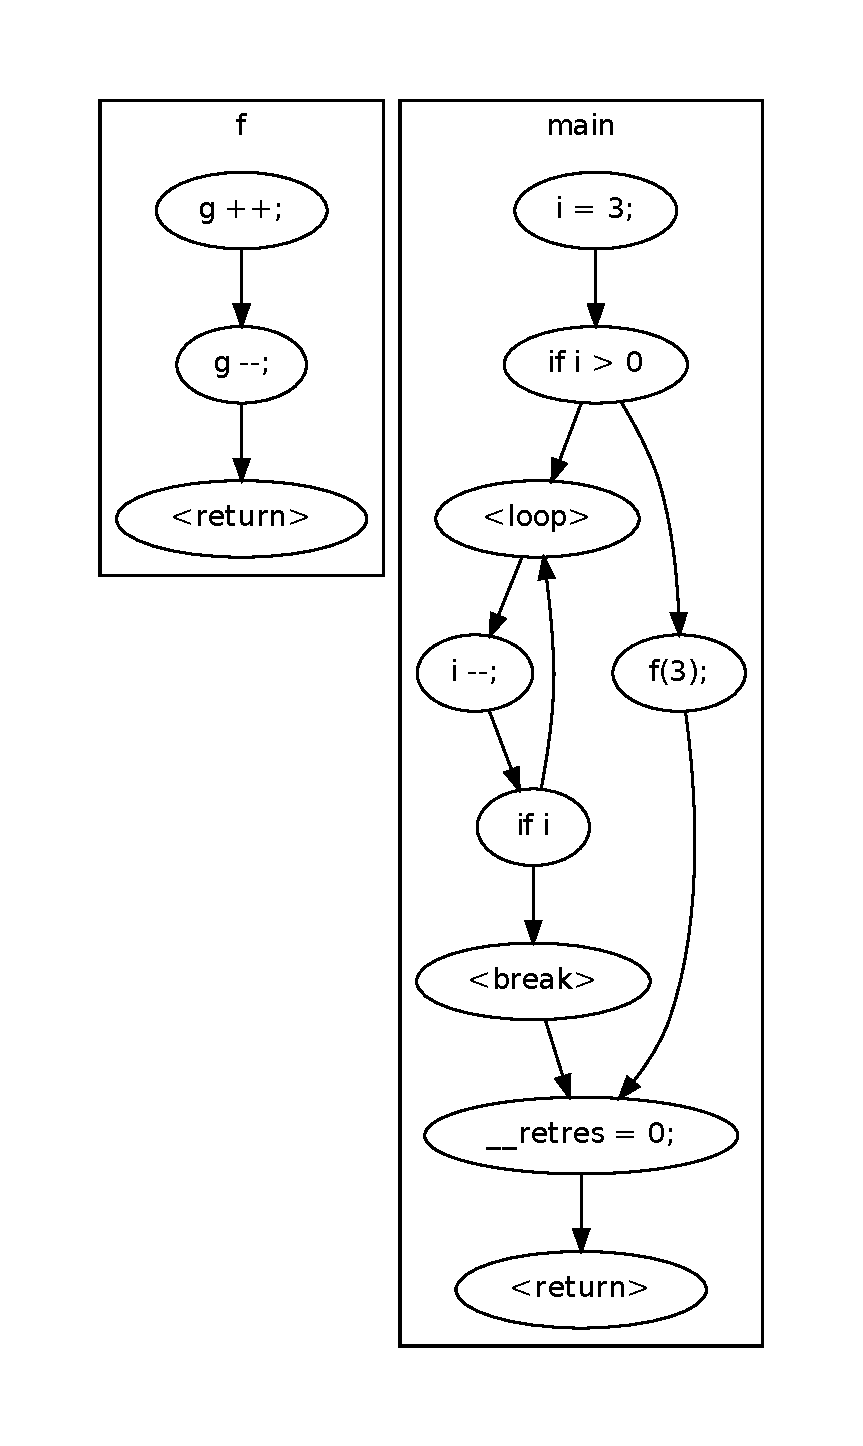
\includegraphics[width=\textwidth]{./tutorial/viewcfg/pdfs/cfg.pdf}
  \end{minipage}

  \caption{Control flow graph for file test.c.}
  \label{fig:tut:basiccfg}
\end{figure}

\subsubsection*{Further improvements}

There are many possible enhancements to this code:

\begin{itemize}
\item There is a bug when trying to print statements that contain
  strings (such as \verb|printf("Hello\n")| such statements must be
  protected using the \verb|"%S"| Format directive;
\item The script could be transformed into a regular plug-in, by
  registering into \framac, and taking options from the command line;
  for instance to compute the control flow graph of a single function
  given as an argument;
\item The graphs could be fancier, in particular by distinguishing
  between branching nodes and plain ones, or showing exit of blocks as
  well as their beginning; or linking a call with the called function.
\end{itemize}

We will concentrate on another extension, which is to reuse the
analysis of the \texttt{value} \framac plug-in to color unreachable
nodes.
To do so, because we will combine different plug-ins, we need to ensure their
correct ordering. This requires the definition of some command-line options.

\subsection{Plug-In registration and command-line options}\label{tut2:options}
\index{Plug-in!Command Line Options}\index{Command Line}

We have already seen how to register options in the previous ``Hello'' tutorial.
We now apply these principles to the ViewCfg plug-in.

\ocamlinput{./tutorial/viewcfg/src/register_and_options.ml}
\scodeidx{Plugin}{Register}
\ocamlinput{./tutorial/viewcfg/src/extend_with_run_with_options.ml}
\scodeidx{Visitor}{visitFramacFileSameGlobals}
\scodeidx{Ast}{get}

We added two options, \texttt{-cfg} to compute the CFG
conditionally (important for ordering plug-in executions),
and \texttt{-cfg-output} to choose the output file.

An interesting addition would be a \texttt{-cfg-target} option,
which would take a set of files or functions whose CFG would be
computed, using the \texttt{Self.Kernel\_function\_set} functor. Depending on
the targets, visiting the AST would have different starting points.
This is left as an exercise for the reader.

Another interesting exercise is to solve the following problem.
Currently, the complete CFG for the whole application is computed in
each \framac step, \ie executing \texttt{frama-c test.c -cfg
  -then -report} would compute the CFG twice. Indeed, the
\texttt{-cfg} option sets \texttt{Enabled} to true, and the
\texttt{run} function is executed once per task. To solve this
problem, one has to create a boolean state to remember that the plug-in
has already been executed. The \texttt{apply\_once} function in the
\texttt{State\_builder} module helps dealing with this issue (reading
the section~\ref{tut2:project-and-state} of this tutorial and
section~\ref{adv:project} of this manual should help you understand the
underlying notion of states).

With these command-line options, we can properly interface our ViewCfg plug-in
with the \texttt{value} plug-in.

\subsection{Interfacing with a kernel-integrated plug-in}

Kernel-integrated plug-ins, such as \texttt{value}, use a special mechanism
to statically register their APIs for other plug-ins that wish to access them.
This mechanism is the \texttt{Db} module of the \framac kernel,
the entry point for all kernel-integrated plug-ins. By using the functions
exported through the \texttt{Db.Value} module, our plug-in will obtain
reachability information computed by \texttt{value}.

The code modification we propose is to color in pink the nodes guaranteed to
be unreachable by the value analysis. For this purpose, we change the
\texttt{vstmt\_aux} method in the visitor:

\ocamlinput{./tutorial/viewcfg/src/print_cfg_vstmt_aux_value.ml}
\sscodeidx{Db}{Value}{is\_computed}
\sscodeidx{Db}{Value}{get\_stmt\_state}
\sscodeidx{Db}{Value}{is\_reachable}
\sscodeidx{Cil}{visitAction}{DoChildren}
\sscodeidx{Visitor}{frama\_c\_visitor}{vstmt\_aux}

This code fills the nodes with green if the node may be
reachable, and in pink if the node is guaranteed not to be
reachable; but only if the value analysis was previously computed. 

To test this code, frama-c should be launched with:
\begin{shell}
  frama-c test.c -load-script cfg_print.ml -val -then -cfg && dotty cfg.out
\end{shell}

Note that the relative order of the parameters \texttt{-load-script} and
\texttt{-val} in this example is not relevant
(see Section~\ref{adv:init} for details).
However, it is important to ensure that \texttt{-cfg} is separated from
\texttt{-val} by a \texttt{-then}; otherwise, it is not guaranteed that
the \texttt{value} plug-in will run before the ViewCfg plug-in, which might
lead to a non-colored graph in some cases, and colored in others.

The resulting graph is shown in Figure~\ref{fig:tut:coloredcfg}.

\begin{figure}[htbp]
  \centering
  \begin{minipage}[h]{0.45\linewidth}
  \listingname{test.c}
  \cinput{./tutorial/viewcfg/tests/test.c}
  \end{minipage}%
  \begin{minipage}[h]{0.4\linewidth}
    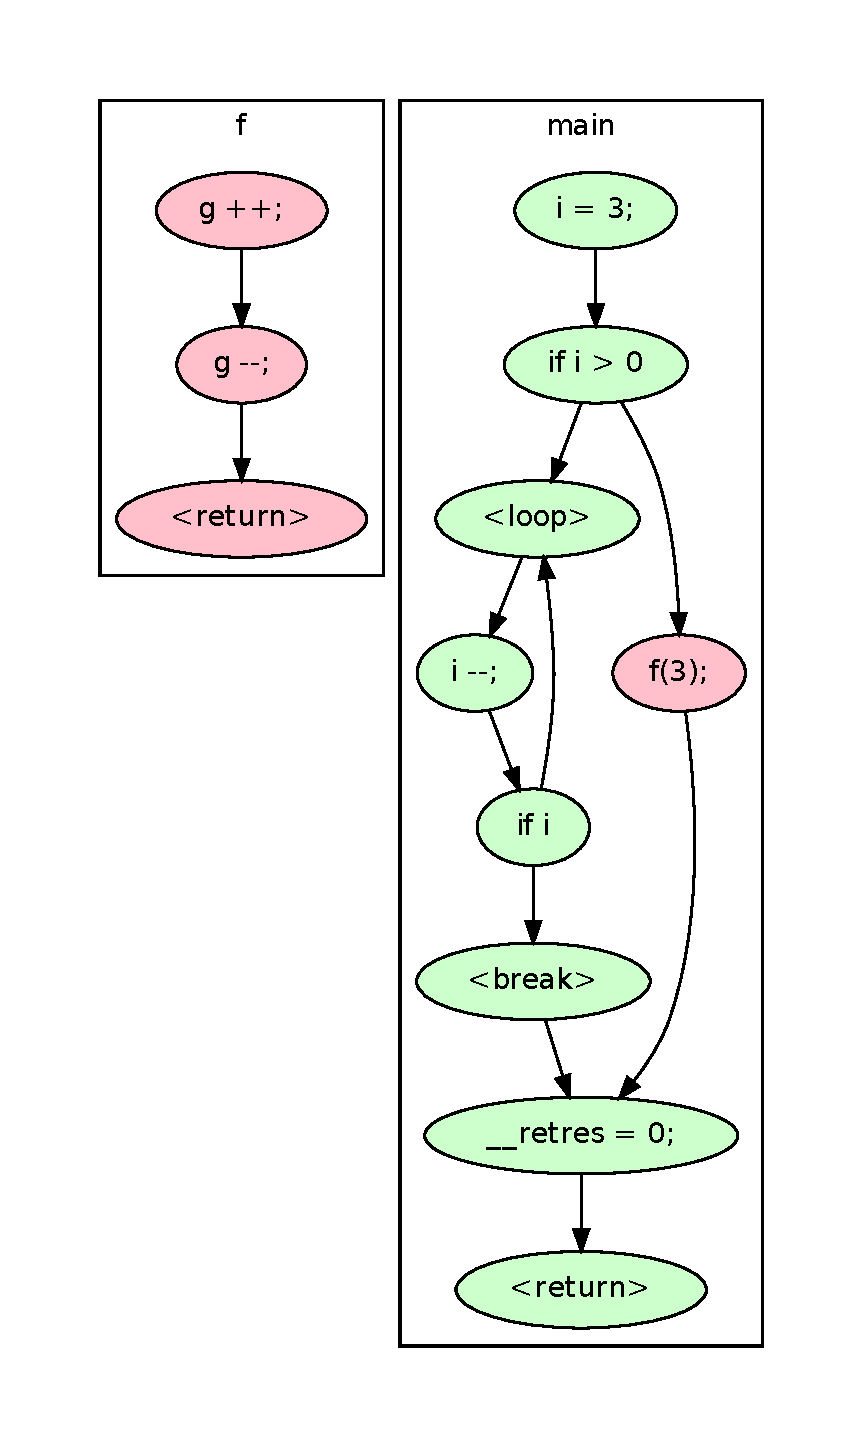
\includegraphics[width=\textwidth]{./tutorial/viewcfg/pdfs/cfg_colored.pdf}
  \end{minipage}
  \caption{Control flow graph colored with reachability information.}
  \label{fig:tut:coloredcfg}
\end{figure}

\subsection{Extending the Frama-C GUI}
\label{tut2:gui}
\index{Plug-in!GUI}

In this section, we will extend our plug-in so that the control flow
graph can be displayed interactively. For that, we will extend the \framac GUI
so that when you right-click on a function in the code, a new ``Show
CFG'' item appears, that displays the control flow graph of the
function in a dialog box. This is achieved just by appending the following
pieces of code at the end of the \texttt{cfg\_print.ml} file.

Currently, we used a visitor that outputs a \dottool file with the CFG of
all functions of all files. We use \texttt{dump\_function} to output
the CFG of a single function instead.

\ocamlinput{./tutorial/viewcfg/src/dump_function.ml}

We reused the \texttt{print\_cfg} visitor, but we selected a different
starting point. The argument \texttt{fundec} gets type
\texttt{Cil\_types.fundec}\scodeidx{Cil\_types}{fundec}, which is the CIL type
representing a function definition.

Now we write the GUI extension code:

\ocamlinput{./tutorial/viewcfg/src/gui.ml}
\scodeidx{Pretty\_source}{PVDecl}
\sscodeidx{Globals}{Functions}{get}
\scodeidx{Kernel\_function}{get\_definition}
\scodeidx{Gtk\_helper}{graph\_window}
\scodeidx{Design}{register\_extension}
\sscodeidx{Design}{main\_window\_extension\_points}{register\_source\_selector}

Let us explain this code from the end. \texttt{Design.register\_extension} is
the entry point for extending the GUI. Its argument is a function which takes as
argument an object corresponding to the main window of the \framac GUI. This
object provides access to the main widgets of the window, and several
extension points.

Here we have implemented a single extension, the ``source selector'',
that allows to add entries to menu obtained when right-clicking on the
source. This is implemented by the \texttt{cfg\_selector} function.

This function takes a \texttt{localizable} argument, which gives information on
where the user clicks on the source. Here we do something only if the user
clicks on the declaration of a variable whose type is a function (\ie when the
user clicked on a function declaration or definition).  In that case, we add an
item to the popup menu, that calls the \texttt{callback} function if
clicked. The \texttt{callback} function calls a \framac GUI function that
displays a graph from \dottool printing functions. It uses several important \framac
APIs: \texttt{Globals} and \texttt{Kernel\_function}, which contain several
functions for manipulating globals and functions.

Note that this GUI extension could also have been done through a script
(instead of a plug-in), but it would have been less than ideal.
In particular, the GUI \ocaml modules are available only when a script
is loaded with \texttt{frama-c-gui}, and not when loaded with
\texttt{frama-c}. When the user wants to view the CFG from the GUI,
outputting the CFG of all functions in \texttt{cfg.out} is useless.
A better architectural solution is to split our plug-in in several files,
with its own Makefile, to better manage its functionalities.

\subsection{Splitting files and writing a Makefile}\label{tut2:makefile}
\index{Plug-in!Makefile}

The \framac plug-in development environment allows to split GUI-related
and non-GUI related modules, so that GUI-related modules are loaded
and run only if \framac is executed with \texttt{frama-c-gui}. This
requires splitting the module into several files. We choose the
following architecture:

\begin{itemize}
\item \texttt{cfg\_options.ml} implements plug-in registration and
  configuration options;
\item \texttt{cfg\_core.ml} implements the main functions for
  computing the CFG;
\item \texttt{cfg\_register.ml} implements ``global'' computation of
  the CFG using the \texttt{-cfg} option, and hooking into the \framac
  main loop;
\item \texttt{cfg\_gui.ml} implements GUI registration.
\end{itemize}

Dependencies between the modules\footnote{This graphic is generated in
  file \texttt{doc/code/modules.dot} after running \texttt{make doc}.}
is presented on Figure \ref{fig:tut:cfgarchitecture}.

\begin{figure}[htbp]
  \centering
    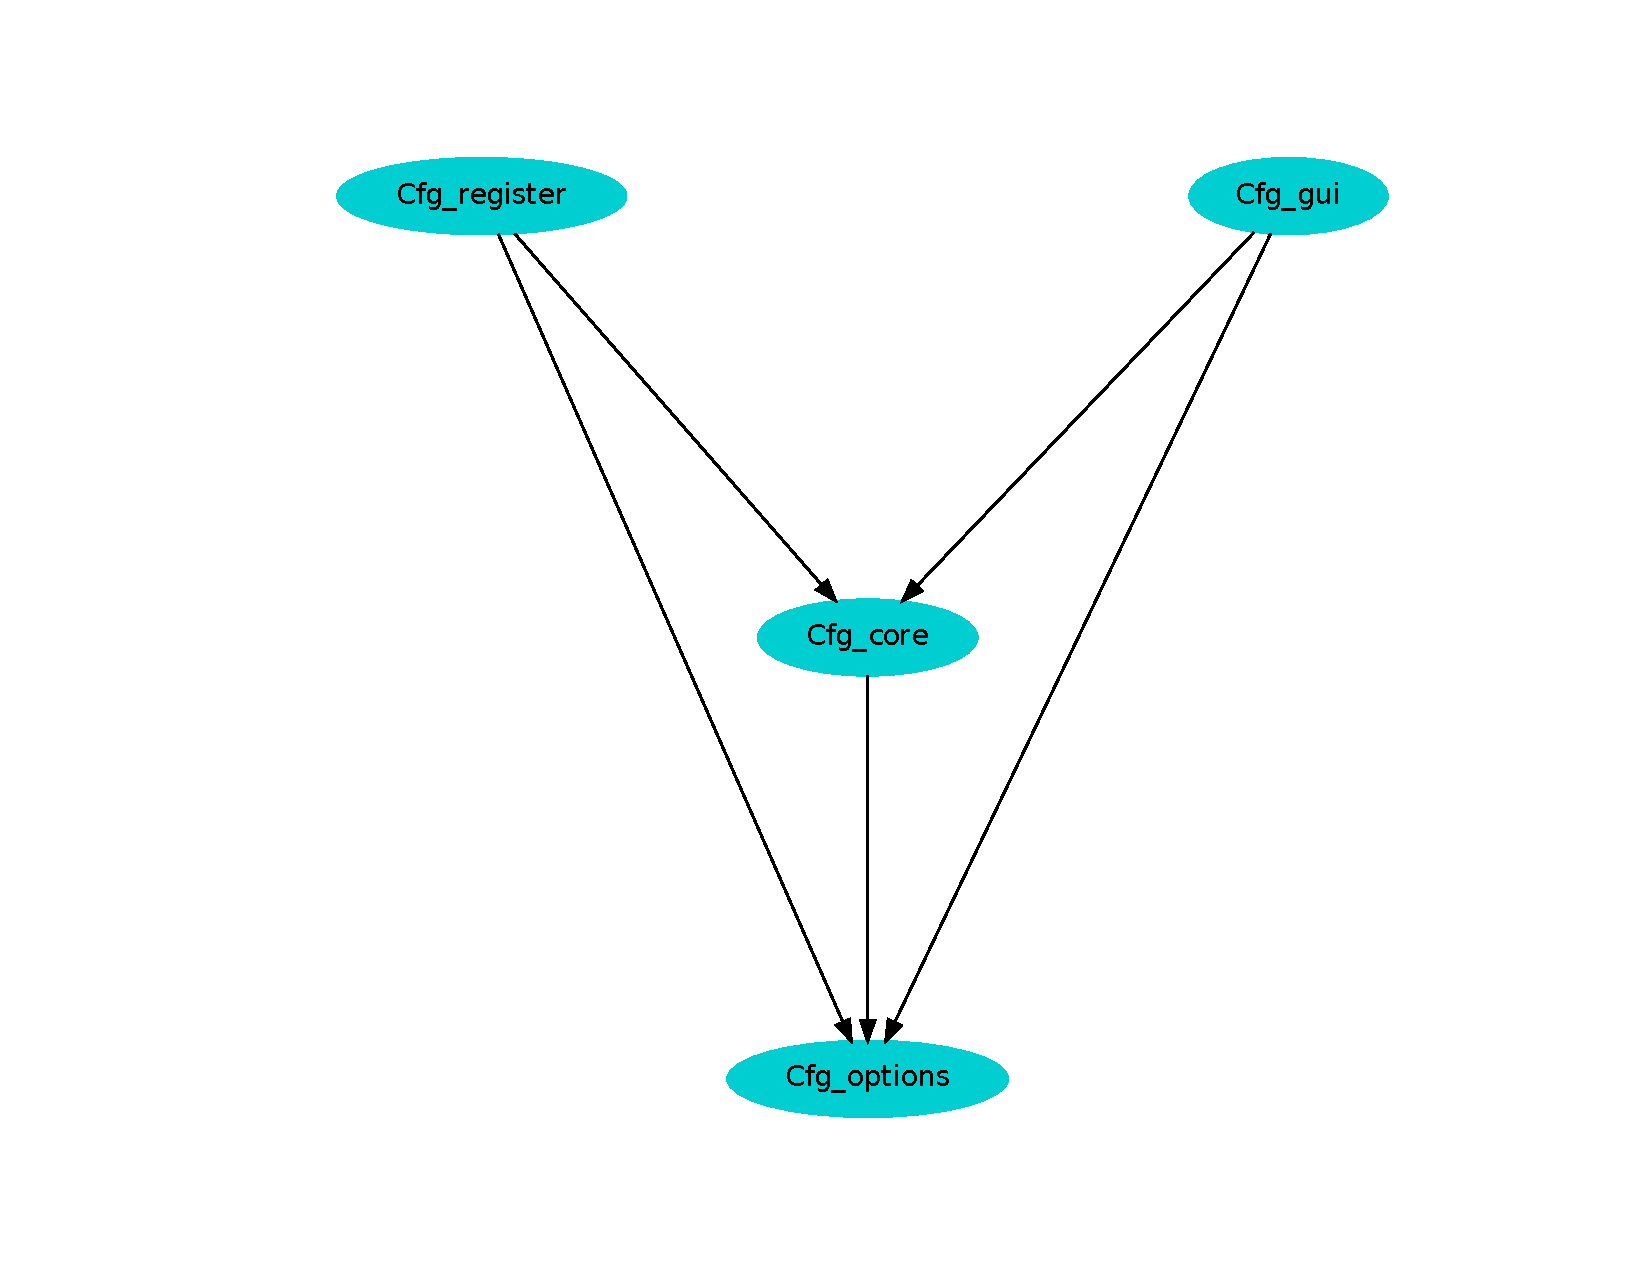
\includegraphics[width=0.5\textwidth]{./tutorial/viewcfg/pdfs/modules.pdf}
  \caption{CFG plug-in architecture}
  \label{fig:tut:cfgarchitecture}
\end{figure}

To break recursive dependencies between \ocaml modules, it is typical
that plug-in registration is done at the bottom of the module
hierarchy, while definition of the \texttt{run} function is at the
top. The GUI is also at the top of the hierarchy: the \framac
\texttt{Makefile} requires that normal plug-in modules do not depend on
GUI modules. Note that currently, the dependency from
\texttt{Cfg\_core} and \texttt{Cfg\_gui} to \texttt{Cfg\_register} is
artificial, but in future evolutions the GUI could depend on
configuration options.

\listingname{Makefile}
\codeidx{Makefile.dynamic}
\codeidx{FRAMAC\_SHARE}
\codeidx{PLUGIN\_CMO}
\codeidx{PLUGIN\_GUI\_CMO}
\codeidx{PLUGIN\_NAME}
\makefileinput{./tutorial/viewcfg/generated/split/Makefile}

In the \texttt{Makefile}, the \texttt{PLUGIN\_CMO} variable must
contain the list of file names of the ml files, in the correct \ocaml
build order. Modules in \texttt{PLUGIN\_CMO} must not depend on modules in
\texttt{PLUGIN\_GUI\_CMO}.

We also need to add an interface for the whole plug-in:
\listingname{ViewCfg.mli}
\ocamlinput{./tutorial/viewcfg/generated/split/ViewCfg.mli}

Here is the listing for the different modules:

\listingname{cfg\_options.ml}
\ocamlinput{./tutorial/viewcfg/generated/split/cfg_options.ml}

\listingname{cfg\_core.ml}
\ocamlinput{./tutorial/viewcfg/generated/split/cfg_core.ml}

\listingname{cfg\_register.ml}
\ocamlinput{./tutorial/viewcfg/generated/split/cfg_register.ml}

\listingname{cfg\_gui.ml}
\ocamlinput{./tutorial/viewcfg/generated/split/cfg_gui.ml}

\subsection{Getting your Plug-in Usable by Others}\label{tut2:api}
\index{Plug-in!API}
\todo

% TODO: A script that uses "dump_function" of the CFG plug-in

\subsection{Writing your Plug-in into the Journal}\label{tut2:journal}
\index{Journalization}
\todo

% TODO: Journalize dump_function.

% La journalisation, c'est le fait d'avoir la GUI rajouter des entrees
% dans le journal, pour pouvoir les rejouer. Ca permet, quand on
% paufine des analyses, de refaire ce qu'on a fait dans la gui
% automatiquement; apres on peut utiliser load-script pour rejouer le
% journal.

% Pour journaliser, il faut enregister la fonction pour qu'elle soit
% accessible de l'exterieur. Apres il y a un argument journalize qui
% permet de journaliser. Si je fais ca pour ma fonction dump_function,
% je vais recuperer une fonction dump_function_journalized; et c'est
% celle ci-qu'il faudrait que j'utilise dans la GUI; comme ca a chaque
% fois que je fais un "show-cfg", ce serait enregistre. La ce n'est
% pas tres interessant parce que je ne fais pas de modification de
% l'AST, mais dans le cas general ca l'est.

\subsection{Writing a Configure Script}\label{tut2:configure}
\index{Plug-in!Configure}
\todo

% Detect \dottool at compile time.
% Link to section 5.3: plug-in specific configure.in

\subsection{Getting your plug-in Usable in a Multi Projects Setting}
\label{tut2:project-and-state}
\index{Project}

\subsubsection{Registering and using state}

In this section, we will learn how to register state into \framac. A
\emph{state} is a piece of information kept by a plug-in. For instance,
the \texttt{value} plug-in computes, for each statement, a table associating to
each AST's variable a set of values the program may have at runtime: this
association table is a state.

State registration provides several features:
\begin{itemize}
\item It allows the state to be saved and reloaded with the rest of
  the session, for instance when using \texttt{frama-c -save/frama-c
    -load};
\item It helps maintaining consistency between the AST and the results and
  parameters of the analysis of the different plug-ins.
\end{itemize}

In this tutorial, we will store the file representing the \dottool
output of the control flow graph of a function (as needed by
\texttt{dump\_function}) as a string, by using a hashtable from \texttt{fundec}
to \texttt{string}. Storing this string will allow us to memoize~\cite{michie68}
our computation: the string is computed the first time the CFG of a
function is displayed, while the following requests will reuse the result of
the computation. Registering the hashtable as a \framac state is
\emph{mandatory} to ensure \framac consistency: for instance, by using a
standard \caml hashtable, a user that would have loaded several session through
the GUI could observe the CFG of function of a previous session instead of the
one he wants to observe.

Registering a state is done by a functor application:

\ocamlinput{./tutorial/viewcfg/src/register_cfg_graph_state.ml}
\scodeidx{State\_builder}{Hashtbl}
\sscodeidx{Cil\_datatype}{Fundec}{Hashtbl}
\scodeidx{Datatype}{String}
\scodeidx{Ast}{self}
\sscodeidx{Db}{Value}{self}

The \texttt{State\_builder} module provides several functors that help
registering states. \texttt{State\_builder.Hashtbl} allows the developer to
create a hashtable. It is parameterized by a module describing the hashtable
and its key, a module describing the data associated to keys, and
other informations. 

The \texttt{Datatype} and \texttt{Cil\_datatype} modules describe the
hashtable and its associated data, and explain for instance how the
datatype should be copied, printed, or marshalled to the disk. They
are part of the \texttt{Type} library~\cite{signoles:jfla11}, described in
Section~\ref{adv:datatype}. \texttt{Datatype} provides
descriptions for standard \caml types, and \texttt{Cil\_datatype} for
the CIL types (in the \texttt{Cil\_types} module).

The last module argument describes the initial size of the hashtable, a name
(mainly used for internal debugging), and a list of \emph{dependencies}. Here we
expressed that our hashtable depends on the Ast and the results of the
\texttt{Value} plug-in. For instance, whenever the \framac kernel updates one of these
states, it will automatically reset our hashtable. This ensures consistency of
the analysis: if the Ast of a function changes, or the value analysis is
executed with a different entry point, this potentially affects the display of
the control flow graph, that we must recompute.

Once the module has been declared, it is fairly easy to use it.

\ocamlinput{./tutorial/viewcfg/src/dump_to_string_memoized.ml}
\scodeidx{Visitor}{visitFramacFunction}
\ocamlinput{./tutorial/viewcfg/src/dump_function_memo_no_clear_cache.ml}

\texttt{dump\_function} now takes two steps: first the CFG is printed
to a string, then the string is printed to the \texttt{fmt}
argument. This allows the \texttt{dump\_to\_string} part to be
\emph{memoized}, \ie the results of \texttt{dump\_to\_string} are
saved so that later calls to \texttt{dump\_function} with the same
\texttt{fundec} argument reuse that result. 

If you launch \texttt{frama-c-gui} with the above code, click on
functions to view their CFG, and inspect the console, you will observe
that the string ``Computing CFG for function ...'' is displayed only
once per function.

One can see the effects of the dependency on the \texttt{Value} plug-in
by first launching the value analysis, inspecting the CFG for the
\texttt{f} function, then changing the entry point to \texttt{f} in the
CFG and re-running the value analysis. The console indicates that the
\texttt{CFG} have been recomputed. Indeed the state of the
\texttt{Value} plug-in, and of its dependencies, was reset when the
entry point was changed.

Another way to observe how \framac automatically handles states is to display a
CFG, save the session, close and restart \framac, 
and then reload the session: the control flow graph is not recomputed,
which means that \framac has automatically saved the
\texttt{Cfg\_graph\_state} with the rest of the session. Everything
should also work properly when loading several sessions.

\subsubsection{Clearing states, selection and projects}

There is one caveat though: if the user computes the CFG before
running the \texttt{Value} analysis, and then runs \texttt{Value}, he
will not see a colored graph (unless he re-launch the \texttt{Value}
analysis with different parameters). This is because the state of the
CFG is reset when the state of \texttt{Value} is reset, not when it is
first computed.

To solve this problem, we will manually reset the
\texttt{Cfg\_graph\_state} if we detect that the \texttt{Value}
analysis has been run since the last time we computed the CFG. For
that, we have to remember the previous value of
\texttt{Db.Value.is\_computed ()}, \ie to register another state:

\ocamlinput{./tutorial/viewcfg/src/register_value_computed_state.ml}
\scodeidx{State\_builder}{Ref}
\scodeidx{Datatype}{Bool}

This new state only consists of a reference to a boolean value.

Then we just replace \texttt{dump\_function} in the code above by the
following.

\ocamlinput{./tutorial/viewcfg/src/dump_function_memo_clear_cache.ml}
\sscodeidx{Db}{Value}{is\_computed}
\scodeidx{State\_selection}{with\_dependencies}
\scodeidx{Project}{clear}

The only part that need to be explained is the notion of
\emph{selection} and \emph{project}. A selection is just a set of
states; here we selected the state \texttt{Cfg\_graph\_state} with all
its dependencies, as resetting this state would also impact states
that would depend on it (even if there is none for now). We use
\texttt{Project.clear} to reset the selection.

\subsubsection{Project explanation}

A \emph{project}~\cite{project} is a consistent version of all the \emph{states}
of \framac. \framac is multi-AST, \ie \framac plug-ins can change the AST of the
program, or perform incompatible analysis (\eg with different entry
points). Projects consistently groups a version of the AST of the program, with
the states related to this AST.

The \texttt{Project.clear} function has type :
\begin{ocamlcode}
val clear: ?selection:State_selection.t -> ?project:t -> unit -> unit  
\end{ocamlcode}
\scodeidxdef{Project}{clear}
\scodeidx{State\_selection}{t}
\scodeidx{Project}{t}

The arguments \texttt{selection} and \texttt{project} can be seen as a
coordinate system, and the function allows to clear specific versions
of specific states. By default, \framac functions act on the
\emph{current} project. The developer has to use \texttt{Project.on} or optional
arguments to act on different projects. \framac automatically handles
duplication and switch of states when duplicating or changing of
projects. This is the last benefit of state registration.

To summarize:

\begin{itemize}
\item To store results, plug-ins should register \emph{states};
\item A \emph{project} is a consistent version of all the states in
  \framac, together with a version of the AST;
\item A \emph{session} is a set of \emph{projects};
\item \framac transparently handles the versioning of states when
  changing or duplicating projects, saving and reloading sessions from
  disk, etc.
\item The version of the state in a project can change; by default
  \framac functions operate on the current project.
\item A \emph{selection} is a set of states. \emph{Dependencies} allow
  to create selections.
\item As a plug-in developer, you have to remember that is up to you to preserve
  consistency between your states and their dependencies by clearing the latter
  when the former is modified in an incompatible way. For instance, it would
  have been incorrect to not call 
  \texttt{State\_selection.with\_dependencies}
  \scodeidx{State\_selection}{with\_dependencies} in the last code snippet of
  this tutorial.
\end{itemize}

Projects are generally created using copy visitors. We encourage the reader to
experiment with multiple projects development by using them. An interesting
exercise would be to change the AST so that execution of each instruction is
logged to a file, and then re-read that file to print in the CFG how much time
each instruction has been executed. Another interesting exercise would be
to use the \texttt{apply\_once} function so that the ViewCfg plug-in is executed
only once, as explained in section~\ref{tut2:options} of this tutorial.

%; whizzy-master "main.tex"

\chapter{Tutorial}\label{chap:tutorial}

\begin{target}beginners.\end{target}

This chapter aims at helping a developer to write his first \framac plug-in. At
the end of the tutorial, any developer should be able to extend \framac with a
simple analysis available as a \framac plug-in. This chapter was written as a
step-by-step explanation on how to proceed towards this goal. It will get you
started, but it does not tell the whole story. You will get it with your own
experiments, and by reading the other chapters of this guide as needed.

First, Section~\ref{tut2:environment} describes how to quickly setup a
development environment for \framac.
Section~\ref{tut2:architecture} shows what a plug-in looks like. Then
Section~\ref{tut2:hello} explains the basis for writing a standard \framac
plug-in\index{Plug-in}, while Section \ref{tut2:cfg} details how to interact
with \framac and other plug-ins to implement analyzers of \C programs.

\section{Quick Setup of a Development Environment}\label{tut2:environment}

This setup is based on Emacs as the IDE, with OPAM for OCaml package
installation and Merlin for OCaml source code navigation.
Similar environments can be setup using other editors, such as Vim and
Sublime Text, but they are not detailed here; please refer to the Merlin
documentation for further details on how to setup other editors for OCaml
development.

\subsection{Emacs Configuration Files}

The \framac source distribution includes, in its \texttt{share} directory,
some \texttt{frama-c-*.el} files ({\em Emacs-lisp} scripts)
with default settings for an OCaml development environment based on
Emacs + OPAM + Merlin. To set it up, do the following:

\begin{enumerate}
\item Install Emacs, OPAM, and OPAM packages \textsf{merlin}, \textsf{tuareg}
  and \textsf{ocp-indent};
\item Copy \texttt{share/emacs/frama-c-*.el} to a directory in your Emacs load-path;
\item Add \texttt{(load-library "frama-c-recommended")} to your \texttt{.emacs}
  init file.
\end{enumerate}

For instance, run these commands (after having installed OPAM):

\begin{verbatim}
opam install merlin tuareg ocp-indent
mkdir ~/.emacs.d/frama-c
cp <path to frama-c sources>/share/emacs/frama-c-*.el ~/.emacs.d/frama-c/
\end{verbatim}

And then add this in the beginning of your \texttt{\textasciitilde/.emacs}:

\begin{verbatim}
(add-to-list 'load-path "~/.emacs.d/frama-c")
(load-library "frama-c-recommended")
\end{verbatim}

You can replace \texttt{frama-c-recommended} with \texttt{frama-c-dev} in the
above line. The former contains some extra, optional settings, while the latter
contains only the most important settings for OCaml development. We recommend
you review the definitions in \texttt{frama-c-recommended} and remove those you
find unnecessary.

\subsection{Quick Merlin guide}

Merlin\footnote{Merlin is available on Github
  (\url{https://github.com/the-lambda-church/merlin}) and as an OPAM package.}
is a tool for OCaml type information, source code navigation and
auto-completion.

Detailed instructions for using Merlin with Emacs are available at
\url{https://github.com/the-lambda-church/merlin/wiki/emacs-from-scratch}.

The \framac Makefile contains a target \textsf{merlin} that generates an
appropriate \texttt{.merlin} file to be used when editing \framac
\texttt{.ml/.mli} files. Run \texttt{make merlin} after compiling \framac,
and the generated \texttt{.merlin} file will be automatically used when opening 
\framac OCaml sources.

Here is a quick summary of the most useful commands when editing
\texttt{.ml/.mli} files:

\begin{itemize}
\item \texttt{Ctrl+c  Ctrl+t}: display type information
  (repeat it to further expand types)
\item \texttt{Ctrl+c  Ctrl+l}: jump to definition
  (for variables, types, modules, etc.)
\item \texttt{Ctrl+c  Ctrl+x}: jump to next error in current buffer
\end{itemize}

Merlin also includes an auto-complete feature. Check its website for
further documentation.

\section{What Does a Plug-in Look Like?}\label{tut2:architecture}
\index{Plug-in!Architecture}\index{Architecture!Plug-in}

Figure~\ref{fig:overview} shows how a plug-in can integrate with the \framac
platform. This tutorial focuses on specific parts of this figure.

\begin{figure}[ht]
\begin{center}
\newsavebox{\designbox}
\savebox{\designbox}{\begin{varwidth}{\textwidth}\centering Design\\(GUI extension point)\end{varwidth}}
\newlength{\designheight}
\setlength{\designheight}{\totalheightof{\usebox\designbox}}
\newsavebox{\captionbox}\savebox{\captionbox}{\textbf{Caption:}}
\newlength{\captionheight}\settototalheight{\captionheight}{\captionbox}
\begin{tikzpicture}[remember picture,txt/.style={inner xsep=3pt}]
  \node[inner sep=0pt] (implem) {
    \tikztitleboxbig{Plug-in\\implementation}{darkgreen}{
      \begin{tikz-vbox}{plugin-text}
        \node[on chain, draw, txt,minimum height=\designheight](register){Register};
        \node[on chain, draw, txt,minimum height=\designheight](options){Options};
        \node[on chain]{
          \begin{tikz-hbox}[every node/.style={minimum height=\designheight,minimum width=\designheight}]{etc-text}
            \node[draw, on chain]{};
            \node[on chain] {\ldots};
            \node[draw, on chain] {};
          \end{tikz-hbox}
        };
      \end{tikz-vbox}
    }
  };
  \node[anchor=south west,inner sep=0pt,xshift=\padding]
    at (implem.south east) (gui){
    \tikztitleboxbig{Plug-in GUI}{darkgreen}{
      \begin{tikz-hbox}{pluginguicontent}
        \begin{scope}[
          every node/.style={
            on chain,
            minimum width=\designheight,
            minimum height=\designheight}]
          \node[draw] {}; \node {\ldots}; \node[draw] {};
        \end{scope}
      \end{tikz-hbox}
    }
  };

  \coordinate[yshift=\padding] (makefile-se) at (gui.north east);
  \coordinate (makefile-nw) at (gui.west |- implem.north);
  \node[fill=palered, rounded corners=5pt,node font=\large,
        fit=(makefile-nw) (makefile-se),
        inner sep=0pt,draw]
        (makefile)
        {Makefile};

   \node[node font={\Large\bfseries},yshift=\padding,anchor=south]
   at ($(implem.north west)!0.5!(makefile.north east)$)
   (plugin-title)
   {Plug-in directory};
   \begin{scope}[on background layer]
     \node[fill=LightCyan, rounded corners=7pt,draw,
           fit=(implem) (gui) (makefile) (plugin-title), inner sep=\padding]
           (plugin-dir)
           {};
   \end{scope}

   \node[anchor=north,yshift=-\bigpadding,fill=Orange,draw]
   at (gui.south|-plugin-dir.south) (design) {\usebox\designbox};

   \node[anchor=north east,
         yshift=-\bigpadding-\captionheight]
   at (plugin-dir.east |- design.south) (registration) {registration points};
   \draw[Latex-] ($(registration.west)+(-\padding,0)$) -- +(-\bigpadding,0);

   \node[anchor=south east,xshift=-\padding] at (registration.north west)
   {\usebox{\captionbox}};

   \node[anchor=south,yshift=\bigpadding,fill=palered,draw,
   minimum height=1.5\designheight]
   at (plugin-dir.north -| gui.north) (makefile-dynamic) {Makefile.dynamic};

   \newlength{\kernelwidth}
   \setlength{\kernelwidth}{\widthof{Dynamic}}%TODO:compute dynamically
   \node[xshift=-\bigpadding,anchor=east] at (plugin-dir.west) {
     \begin{tikz-vbox}[every node/.style=
       {on chain,draw,fill=Orange,minimum height=\designheight,txt,
         minimum width=\kernelwidth}]
       {kernel}
       \node (db-main) {Db.Main};
       \node (dynamic) {Dynamic};
       \node (plugin)  {Plugin};
       \node (type)    {Type};
       \node (journal) {Journal};
       \node (project) {Project};
     \end{tikz-vbox}
   };

   \draw[-Latex] (makefile.north) -- (makefile-dynamic.south);
   \draw[-Latex] (gui.south) -- (design.north);
   \coordinate (main-pt) at ($(db-main.east)+(0.9\bigpadding,0)$);
   \draw (register.west) -| (main-pt);
   \draw[-Latex] (main-pt) -- (db-main.east);
   \draw[-Latex] (main-pt |- dynamic.east) -- (dynamic.east);

   \draw[-Latex] (options.west) -- (options.west -| main-pt)
                 -- +(-0.2\bigpadding,0) |- (plugin.east);

   \coordinate (implem-pt) at
   ($(options.west -| main-pt)+(-0.4\bigpadding,-\padding)$);
   \draw (implem-pt -| implem.west) -- (implem-pt);
   \draw[-Latex] (implem-pt) |- (type.east);
   \draw[-Latex] (implem-pt) |- (journal.east);
   \draw[-Latex] ($(plugin-dir.west |- implem-pt)+(0,-\padding)$)
      -- ($(implem-pt)+(0.2\bigpadding,-\padding)$) |- (project.east);

 \end{tikzpicture}
\end{center}
\scodeidx{Db}{Main}\codeidx{Dynamic}\codeidx{Plugin}
\codeidx{Project}\codeidx{Type}\codeidx{Journal}
\codeidx{Makefile.dynamic}\codeidx{Design}
\index{GUI}\index{Plug-in!GUI}
\caption{Plug-in Integration Overview.}\label{fig:overview}
\end{figure}

The implementation of the plug-in is provided inside a specific directory.
The plug-in registers with the \framac platform through
kernel-provided registration points. These
registrations are performed  through hooks\index{Hook} (by applying
a function or a functor). For instance,
the next section shows how to:
\begin{itemize}
\item extend the \framac entry point\index{Entry point} thanks to the function
  \texttt{Db.Main.extend}\sscodeidx{Db}{Main}{extend} if you want to run
  plug-in specific code whenever \framac is executed;
\item use specific plug-in services provided by the module
  \texttt{Plugin}\codeidx{Plugin}, such as adding a new \framac option.
\end{itemize}

\section{The Hello plug-in}\label{tut2:hello}

This simple plug-in explain how to make your plug-in interact basically
with several aspects of the \framac framework: registration, getting
command-line options, compilation and installation, console output,
testing, and documentation. (In case of difficulty, it is explained at
the end of this section how to generate the whole plug-in.)

\subsection{A Simple Script}\label{tut2:script}
\index{Plug-in!Script}

The easiest way to extend \framac is to write a simple script. A
simple 'Hello World' script consists of a single \ocaml file:

\listingname{./hello\_world.ml\footnotemark}
\ocamlinput{./tutorial/hello/generated/script/hello_world.ml}
\sscodeidx{Db}{Main}{extend} 

This script defines a simple function that writes a message to an
output file, then registers the function \texttt{run} as an entry point for the
script. \framac will call it among the other plug-in entry points if the script
is loaded.

The script is compiled, loaded and run with the command
\texttt{frama-c -load-script hello\_world.ml}. Executing this command
creates a \texttt{hello.out} file in the current directory.

\subsection{Registering a Script as a Plug-in}\label{tut2:plugin}
\index{Plug-in!Registration}

To make this script better integrated into \framac, its code must register
itself as a plug-in. Such a registration provides general services, such as
outputting on the \framac console, or extending \framac with new command-line
options.

Registering a plug-in is achieved through the use of the
\texttt{Plugin.Register} functor:

\listingname{./hello\_world.ml}
\ocamlinput{./tutorial/hello/generated/with_registration/hello_world.ml}
\sscodeidx{Db}{Main}{extend}
\scodeidx{Plugin}{Register}

The argument for this functor is a module with three values:
\begin{itemize}
\item \texttt{name} is an arbitrary, non-empty string containing the full name
  of the module.
\item \texttt{shortname} is a small string containing the short name of the
  module, usually used as a prefix for plug-in options. No space is allowed in
  that string.
\item \texttt{help} is a string containing free-form text, containing a
  description of the module.
\end{itemize}

Visible results of the registration include:
\begin{itemize}
\item ``hello world'' appears in the list of available plug-ins
  (consultable with \texttt{frama-c -load-script
    hello\_world.ml -plugins});
\item default options for the plug-in work, including the inline help
  (available with \texttt{frama-c -load-script
    hello\_world.ml -hello-help}).
\end{itemize}

\subsection{Displaying Messages}\label{tut2:messages}
\index{Plug-in!Messages}

The signature of the module \texttt{Self} obtained by applying
\texttt{Plugin.Register} is \texttt{General\_services}. One of these general
services is logging, \ie message display. In \framac, one should never attempt
to write messages directly to \texttt{stderr} or \texttt{stdout}: use the
general services instead\footnote{However writing to a new file using standard
  \ocaml primitives is OK.}.

\listingname{./hello\_world.ml}
\ocamlinput{./tutorial/hello/generated/with_log/hello_world.ml}
\sscodeidx{Db}{Main}{extend}
\scodeidx{Plugin}{Register}

Running this script yields the following output:
\begin{shell}
\$ frama-c -load-script hello_world.ml
[hello] Hello, world!
[hello] 11 * 5 = 55
\end{shell}

The \texttt{result} routine is the function to use to output results of your
plug-in. The \framac output routines takes the same arguments than the \caml
function \texttt{Format.printf}.

The function \texttt{feedback} outputs messages that show progress to the
user. In this example, we gave to feedback a log level of 2, because
we estimated that in most case the user is not interested in seeing
the progress of a fast operation (simple multiplication). The default
log level is 1, so by default this message is not displayed. To see
it, the verbosity of the \texttt{hello} plug-in must be increased:

\begin{shell}
\$ frama-c -load-script hello_world.ml -hello-verbose 2
[hello] Hello, world!
[hello] Computing the product of 11 and 5...
[hello] 11 * 5 = 55
\end{shell}

For a comprehensive list of the logging routines and options, see
Section~\ref{adv:log}.

\subsection{Adding Command Line Options}\label{tut2:basic-options}
\index{Plug-in!Command Line Options}\index{Command Line}

We now extend the \texttt{hello world} plug-in with new options.

If the plug-in is installed (with \texttt{make install}), it will be loaded and
executed on every invocation of \texttt{frama-c}, which is surely not what you
want. To avoid this behavior, we add a boolean option, set by default to false,
that conditionally enables the execution of the main function of the plug-in
(the usual convention for the name of the option is to take the short name of
the module with no suffix, \ie \texttt{-hello} in our case).

We also add another option, \texttt{-hello-output}, that takes a string
argument. When set, the hello message is displayed in the file given as
argument.

\listingname{./hello\_world.ml}
\ocamlinput{./tutorial/hello/generated/with_options/hello_world.ml}

Registering these new options is done by calling the \texttt{Self.False} and
\texttt{Self.String} functors, which respectively creates a new boolean option
whose default value is false and a new string option with a user-defined default
value (here \texttt{"-"}). The values of these options are obtained \via
\texttt{Enabled.get ()} and \texttt{Output\_file.get ()}. 

With this change, the hello message is displayed only if \framac is
executed with the \texttt{-hello} option.
\begin{shell}
\$ frama-c
\$ frama-c -load-script hello_world.ml -hello
[hello] Hello, world!
\$ frama-c -load-script hello_world.ml -hello -hello-output hello.out
\$ ls hello.out
hello.out
\end{shell}

These new options also appear in the inline help for the hello plug-in:
\begin{shell}
\$ frama-c -load-script hello_world.ml -hello-help
...
***** LIST OF AVAILABLE OPTIONS:

-hello              when on (off by default), output a warm welcome message
                    to the user (opposite option is -no-hello)
-hello-output <output-file>  file where the message is output (default:
                    output to the console)
...
\end{shell}


\subsection{Writing a Makefile}\label{tut2:basic-makefile}
\index{Plug-in!Makefile}

The use of \texttt{load-script} is ideal for small experimentations,
or when writing very specific extensions. When a plug-in becomes larger,
or more general-purpose, and must be split into several files, it is a
good idea to build and install it properly. \framac provides means to
simplify this through the use of \texttt{Makefile}s.

First, lets us create a \texttt{hello} directory that will contain all
of our plug-in files. We put \verb+hello_world.ml+ inside it, and then
create our \texttt{Makefile} there.

\subsubsection*{A simple Makefile}

% TODO: Recuperer toutes les informations du tutoriel 1

We write a simple \texttt{./Makefile} for our
\texttt{./hello\_world.ml} plug-in:

\listingname{./Makefile}
\codeidx{Makefile.dynamic}
\codeidx{FRAMAC\_SHARE}
\codeidx{PLUGIN\_CMO}
\codeidx{PLUGIN\_NAME}
\makefileinput{./tutorial/hello/generated/makefile_single/Makefile}

This \texttt{Makefile} sets some variables before including the generic
\texttt{Makefile.dynamic} which is installed within \framac. It may be
customized in several ways to help building a plug-in (see
Section~\ref{adv:dynamic-make} for details).

\begin{important}
  The name of each compilation unit (here \texttt{hello\_world}) must be
  different from the plug-in name set by the \texttt{Makefile} (here
  \texttt{Hello}), from any other plug-in names (\eg \texttt{value}\footnote{
    \texttt{value} is the technical plug-in name of the \texttt{Eva} plug-in})
    and from any other \framac kernel \caml files (\eg \texttt{plug-in}).
\end{important}

The plug-in also needs an interface file. Indeed, thanks to
\texttt{Makefile.dynamic}, each plug-in is packed into a single module
\texttt{\$(PLUGIN\_NAME)}\codeidx{PLUGIN\_NAME} (here \texttt{Hello}) which
needs an interface. Here we simply export an empty interface in order to hide
the whole implementation to other developers.

\listingname{./Hello.mli}
\ocamlinput{./tutorial/hello/src/Hello.mli}
\begin{important}
  Note the unusual capitalization of the filename \texttt{Hello.mli} which is
  required for compilation purposes.
\end{important}

Inside the plug-in's directory, run \texttt{make} to compile it. Note that the
compiled files are copied into a \texttt{top} (for {\em top-level}) subdirectory
(if our plug-in had GUI-dependent modules, they would be placed in a
\texttt{gui} subdirectory).
The module can then be loaded and executed by using
\texttt{frama-c -load-module top/Hello}.

Then run \texttt{make install} to install the plug-in (you need to have write
access to the \texttt{plugins} directory, located at the path given by the
command \texttt{frama-c-config -print-libpath}).

Just launch \texttt{frama-c} (without any option): the \texttt{Hello}
plug-in is now always loaded, without the need to pass other options to
the command line. Check it with the command \texttt{frama-c -hello-help}.

\subsubsection*{Splitting your source files}

Here is a slightly more complex example where the plug-in has been split into
several files. Usually plug-in registration through \texttt{Plugin.Register}
should be done at the bottom of the module hierarchy, while registration of the
run function through \texttt{Db.Main.extend} should be at the top, as in the
following example. The \texttt{PLUGIN\_CMO} variable must contain the list of
file names, in the correct \ocaml build order.

\listingname{./Makefile}
\codeidx{Makefile.dynamic}
\codeidx{FRAMAC\_SHARE}
\codeidx{PLUGIN\_CMO}
\codeidx{PLUGIN\_NAME}
\makefileinput{./tutorial/hello/generated/makefile_multiple/Makefile}

The three following files completely replace the \texttt{./hello\_world.ml}
from the previous section. Modules are directly called by their name in the
classical \ocaml way.

\listingname{./hello\_options.ml}
\ocamlinput{./tutorial/hello/generated/makefile_multiple/hello_options.ml}
\scodeidx{Plugin}{Register}

\listingname{./hello\_print.ml}
\ocamlinput{./tutorial/hello/generated/makefile_multiple/hello_print.ml}

\listingname{./hello\_run.ml}
\ocamlinput{./tutorial/hello/generated/makefile_multiple/hello_run.ml}
\sscodeidx{Db}{Main}{extend}

The plug-in can be tested again by running:

\begin{shell}
\$ make
\$ make install
<...>
\$ frama-c -hello -hello-output hello.out
\$ more hello.out
Hello, world!
\end{shell}

However, this does not consist in a proper test \emph{per se}. The next section
presents how to properly test plug-ins.

\subsection{Testing your Plug-in}\label{tut2:testing}
\index{Plug-in!Testing}\index{Test}

Frama-C supports non-regression testing of plug-ins. This is useful to check
that further plug-in modifications do not introduce new bugs. The tool allowing
to perform the tests is called \ptests\index{Ptests}.

To build these tests, the location of the subdirectories containing them must
be indicated in the \texttt{Makefile} through the variable
\texttt{PLUGIN\_TESTS\_DIRS}\codeidx{PLUGIN\_TESTS\_DIRS} set at
\texttt{hello} as this will be the name of the
subdirectory of \texttt{.tests/} where the plug-in's tests will be located:

\listingname{./Makefile}
\codeidx{Makefile.dynamic}
\codeidx{FRAMAC\_SHARE}
\codeidx{PLUGIN\_CMO}
\codeidx{PLUGIN\_NAME}
\codeidx{PLUGIN\_TESTS\_DIRS}
\makefileinput{./tutorial/hello/generated/with_test/Makefile}

This enables the creation of a
\texttt{./tests/ptests\_config} file holding the environement needed by
\ptests to run the plug-in's tests by running:
\begin{shell}
\$ mkdir tests
\$ make
<...>
Generating   tests/ptests_config
\end{shell}

For non-regression testing, the current behaviour of a program is taken as
the oracle against which future versions will be tested. In this tutorial, the
test will be about the correct \texttt{Hello, world!} output made by the option
\texttt{-hello} of the plug-in.

Each test directory must contain a
\texttt{run.config}\index{Test!Configuration}\index{Test!Header}
comment with the test directives\index{Test!Directive} and the C
source code used for the test.
(There are other ways to declare and control tests as developed
in Section~\ref{ptests:configuration}.)
For this tutorial, there will be no such source code. A file
\texttt{./tests/hello/hello\_test.c} is then created:

\listingname{./tests/hello/hello\_test.c}
\nscodeidx{Test!Directive}{OPT}
\lstinputlisting[style=c]{./tutorial/hello/generated/with_test/tests/hello/hello_test.c}

In this file, there is only one directive
\texttt{OPT: -hello}\nscodeidx{Test!Directive}{OPT} which requires
to run \framac on this test with the \texttt{-hello} option.
A look at Section~\ref{ptests:directives} gives you an idea of the kind of
directives which can be used to test plug-ins.

Once the \texttt{run.config} has been configured, it becomes possible to
get the output generated by the plug-in:
\begin{shell}[breaklines=true]
\$ ptests.opt -show
Env:
<...>
Command:
/usr/local/bin/frama-c.byte tests/hello/hello_test.c -check  -hello 2>tests/hello/result/hello_test.err.log >tests/hello/result/hello_test.res.log
[kernel] Parsing FRAMAC_SHARE/libc/__fc_builtin_for_normalization.i (no preprocessing)
[kernel] Parsing tests/hello/hello_test.c (with preprocessing)
[hello] Hello, world!
Env:
<...>
Command:
<...>
\end{shell}
The option \texttt{-show} runs the tests and shows the output
(but not their examination). Other options are detailed
in Section~\ref{ptests:options} to give a better idea of the
extent to which \ptests is configurable.
Under \texttt{Env} is displayed the context (coming from the file
\texttt{./hello/ptests\_config}).
Then, \texttt{Command} shows the executed command for this test case followed
by bash pipes to control the dataflow. (Note the \texttt{-hello}
option which has been passed to \framac as requested by \texttt{OPT: -hello}
in the \texttt{run.config}.)
Two outputs are considered as results for each test:
an \emph{error} output and a \emph{result} output.
These outputs are logged in the two following files:
\texttt{./tests/hello/result/hello\_test.err.log} and
\texttt{./tests/hello/result/hello\_test.res.log}.
The three lines beginning by \texttt{[kernel]} and \texttt{[hello]}
are the actual non-erroneous outputs made by \framac: two of them are generated
by the kernel (which could be muted by changing the verbosity) while the third
one is generated by our plug-in \texttt{Hello}. \texttt{Env} and
\texttt{Command} parts appear once again because some test strategies need it,
which is not the case in the simple setting of this tutorial.

Once you have verified the output is as expected, set it as an
oracle to be used for later non-regression tests by running:
\begin{shell}
\$ ptests.opt -update
\end{shell}
This command copies the two log files to
\texttt{./tests/hello/oracle/hello\_test.err.oracle} and
\texttt{./tests/hello/oracle/hello\_test.res.oracle}.

The setting of this test case is now finished.
Let's now assume the plug-in is later erroneously modified as follows:

\listingname{./hello\_run.ml}
\ocamlinput{./tutorial/hello/generated/with_test/hello_run_bug.ml}
\sscodeidx{Db}{Main}{extend}

where \texttt{Hello, world!} is incorrectly changed to \texttt{Hello world!}.
Running the command:
\begin{shell}[breaklines=true]
\$ make
<...>
\$ make tests
TESTING PLUG-IN Hello
% Dispatch finished, waiting for workers to complete
Env:
<...>
Command:
<...>
% Comparisons finished, waiting for diffs to complete
--- tests/hello/oracle/hello_test.res.oracle    2017-06-02 14:39:49.407624816 +0200
+++ tests/hello/result/hello_test.res.log       2017-06-02 14:40:03.483624679 +0200
@@ -1,3 +1,3 @@
 [kernel] Parsing FRAMAC_SHARE/libc/__fc_builtin_for_normalization.i (no preprocessing)
 [kernel] Parsing tests/hello/hello_test.c (with preprocessing)
-[hello] Hello, world!
+[hello] Hello world!
% Diffs finished. Summary:
Run = 1
Ok   = 1 of 2
Time = 0.380000 s.
real 0.45
user 0.38
sys 0.03
\end{shell}
displays the differences (à la \texttt{diff}) between the current executions
and the saved oracles. Here the diff clearly shows that the only difference is
the missing comma in the generated message due to our (erroneous) modification.
One test is marked as being successful: that is the test comparing
\texttt{stderr} (which contains an empty string). After fixing the \ocaml code,
running \texttt{make \&\& make tests} again shows that all test cases are
successful.

You may use other \framac's plug-ins as examples of how to integrate a
plug-in with \ptests. Small plug-ins such as \texttt{Report} and
\texttt{Variadic} are good examples (see directories
\texttt{src/plugins/report/tests/} and \texttt{src/plugins/variadic/tests/}).
Please note \framac offers no particular support for other kinds of testing
purposes, such as test-driven development (TDD)\footnote{For the purpose of
driving the development of a plug-in, one should have to manually create
\texttt{./tests/*/oracle/*.err.oracle} and
\texttt{./tests/*/oracle/*.res.oracle} files for example.} for instance.
Additional information about plug-in testing is available in
Sections~\ref{adv:ptests} and~\ref{sec:ptests}.

\subsection{Documenting your Source Code}
\label{tut2:doc}
\index{Plug-in!Documentation}

\framac automatically generates the documentation of plug-ins when the command
\texttt{make doc} is run\footnote{Frama-C kernel needs to have been
installed with code documentation support. If this was not the case, you can
run \texttt{make doc install-doc-code} in Frama-C's main directory as hinted
by the error message appearing in the terminal before trying again to generate
the documentation of the plug-in.}. This relies on \ocamldoc and
requires the plug-in to be documented following the \ocamldoc guidelines
(please refer to the corresponding chapter in \cite{caml}).

We show here how the Hello plug-in could be slightly documented and use
\ocamldoc features such as @-tags and cross references:

\listingname{./hello\_options.ml}
\ocamlinput{./tutorial/hello/generated/with_doc/hello_options.ml}
\scodeidx{Plugin}{Register}

\listingname{./hello\_print.ml}
\ocamlinput{./tutorial/hello/generated/with_doc/hello_print.ml}

\listingname{./hello\_run.ml}
\ocamlinput{./tutorial/hello/generated/with_doc/hello_run.ml}
\sscodeidx{Db}{Main}{extend}

The documentation files of the plug-in are added to
\texttt{./doc/code/} and the link to this
is added to the plug-ins index file
\texttt{./doc/code/index.html}.

This simple tutorial now comes to its end. It focused on the standard features of
architectures and interfaces of \framac plug-ins. A companion archive
\texttt{hello.tar.gz} is available in the download section of the \framac
website\footnote{The direct link is: \url{http://frama-c.com/download.html}.}.
The next tutorial will make you dive in \C analysis.

%%%%%%%%%%%%%%%%%%%%%%%%%%%%%%%%%%%%%%%%%%%%%%%%%%%%%%%%%%%%%%%%%%%%%%%%%%%%%%%%

\section{The ViewCfg plug-in}\label{tut2:cfg}

In this section, we create a new ViewCfg plug-in that computes the control
flow graph of a function and outputs it in the \dottool format. Through its
implementation, we explain some of \framac APIs such as how to visit
an AST\footnote{Abstract Syntax Tree}, to hook a plug-in, to interface
a plug-in with other plug-ins, to extend the
GUI\footnote{Graphical User Interface}, to make a plug-in usable by
others, to make write a plug-in into the journal, to configure a script,
and to make a plug-in usable in a multi-projects setting.

This section assumes the reader is already familiar with the basics of plug-ins
for \framac as covered by the Hello plug-in in the previous
section.

\subsection{Visiting the AST}\label{tut2:visitor}
\index{Visitor}

Writing an analysis for \C programs is the primary purpose of a \framac
plug-in. That usually requires to visit the AST to compute information for some
\C constructs. There are two different ways of doing that in \framac:
\begin{itemize}
\item through a direct recursive descent; or
\item by using the \framac visitor.
\end{itemize}
The first case is usually better if you have to compute information for most \C
constructs, while the latter is better if only few \C constructs are interesting
or if you have to write a program transformation. Of course, it is also possible
to combine both ways to tune it to specific needs.

\subsubsection*{Pretty-printing with direct recursive descent}

Frama-C already has a function to pretty-print statements (namely
\texttt{Printer.pp\_stmt}\scodeidx{Printer\_api}{S.pp\_stmt}), but it is not suitable
for us, as it will recursively print substatements of compound statements
(blocks, if, while, ...) while we only want to pretty print the node representing the
current statement: substatements will be represented by other nodes. Thus we
will use the following small function:
\ocamlinput{./tutorial/viewcfg/src/print_stmt.ml}
\sscodeidx{Cil\_types}{stmtkind}{Instr}
\sscodeidx{Cil\_types}{stmtkind}{Return}
\sscodeidx{Cil\_types}{stmtkind}{Goto}
\sscodeidx{Cil\_types}{stmtkind}{Break}
\sscodeidx{Cil\_types}{stmtkind}{Continue}
\sscodeidx{Cil\_types}{stmtkind}{If}
\sscodeidx{Cil\_types}{stmtkind}{Switch}
\sscodeidx{Cil\_types}{stmtkind}{Loop}
\sscodeidx{Cil\_types}{stmtkind}{Block}
\sscodeidx{Cil\_types}{stmtkind}{UnspecifiedSequence}
\sscodeidx{Cil\_types}{stmtkind}{TryFinally}
\sscodeidx{Cil\_types}{stmtkind}{TryExcept}
\scodeidx{Printer\_api}{S.pp\_instr}
\scodeidx{Printer\_api}{S.pp\_exp}

The \texttt{Cil\_types} module contains the definition of the AST of a \C
program, like constructors \texttt{Cil\_types.Instr},
\texttt{Cil\_types.Return}, and so on which are of type
\texttt{Cil\_types.stmtkind}. The \texttt{Printer} module contains
functions that prints the different Cil types. The documentation of these module
is available on the \framac website\footnote{From
  \url{http://frama-c.com/download.html}.}, or by typing \texttt{make doc} in
the \framac source distribution.

\subsubsection*{Creating the graphs with a visitor}

In order to create our output, we must make a pass through the whole
AST. An easy way to do that is to use \framac visitor mechanism. A
visitor is a class with one method per type of the AST, whose default
behavior is to just call the method corresponding to each of its
children. By inheriting from the visitor, and redefining some of the
methods, one can perform actions on selected parts of the AST, without
the need to traverse the AST explicitly.

\ocamlinput{./tutorial/viewcfg/src/print_cfg_begin.ml}
\scodeidx{Visitor}{frama\_c\_inplace}

Here we used the so-called ``in place'' visitor, which should be used for
read-only access to the AST. When performing code transformations, a
``copy'' visitor should be used, that creates a new project (see
section~\ref{sec:visitors-projects}).

There are three kinds of nodes where we have something to do. First,
at the file level, we create the whole graph structure.

\ocamlinput{./tutorial/viewcfg/src/print_cfg_vfile.ml}
\sscodeidx{Cil}{visitAction}{DoChildrenPost}
\sscodeidx{Cil}{cilVisitor}{vfile}

\texttt{Cil.DoChildrenPost} is one of the possible
\texttt{visitAction}, that tells the visitor what to do after the
function is executed. With \texttt{DoChildrenPost func}, the \texttt{func}
argument is called once the children have been executed: here we close the
parenthesis once that all functions have been printed in the file.

Then, for each function, we encapsulate the CFG in a subgraph, and do
nothing for the other globals.

\ocamlinput{./tutorial/viewcfg/src/print_cfg_vglob.ml}
\sscodeidx{Cil}{visitAction}{DoChildrenPost}
\sscodeidx{Cil}{visitAction}{SkipChildren}
\sscodeidx{Visitor}{frama\_c\_visitor}{vglob\_aux}
\scodeidx{Cil\_types}{GFun}
\scodeidx{Printer\_api}{S.pp\_varinfo}

\texttt{Cil.SkipChildren} tells the visitor not to visit the children
nodes, which makes it more efficient\footnote{In a copying visitor,
\texttt{Cil.JustCopy}\sscodeidx{Cil}{visitAction}{JustCopy}
should have been used instead.}.

Last, for each statement, we create a node in the graph, and create
the edges toward its successors:

\ocamlinput{./tutorial/viewcfg/src/print_cfg_vstmt_aux_novalue.ml}
\sscodeidx{Cil}{visitAction}{DoChildren}
\sscodeidx{Visitor}{frama\_c\_visitor}{vstmt\_aux}

This code could be optimized, for instance by replacing the final
\texttt{DoChildren} by \texttt{SkipChildren} for statements that
cannot contain other statements, like \texttt{Instr}, and avoid
visiting the expressions.

Finally we close the \texttt{object} definition:
\ocamlinput{./tutorial/viewcfg/src/print_cfg_end.ml}

\subsubsection*{Hooking into \framac}

It just remains to hook this script into \framac.

\ocamlinput{./tutorial/viewcfg/src/extend_with_simple_run.ml}

Assuming the script is called \texttt{cfg\_print.ml}, it can then be run with:
\begin{shell}
  frama-c -load-script cfg_print.ml [other_options] file.c [file2.c] 
\end{shell}

And the graph can be visualized with 
\begin{shell}
  dotty cfg.out
\end{shell}

This produces a graph like in Figure~\ref{fig:tut:basiccfg}

\begin{figure}[htbp]
  \centering
  \begin{minipage}[h]{0.45\linewidth}
  \listingname{test.c}
  \cinput{./tutorial/viewcfg/tests/test.c}
  \end{minipage}%
  \begin{minipage}[h]{0.4\linewidth}
    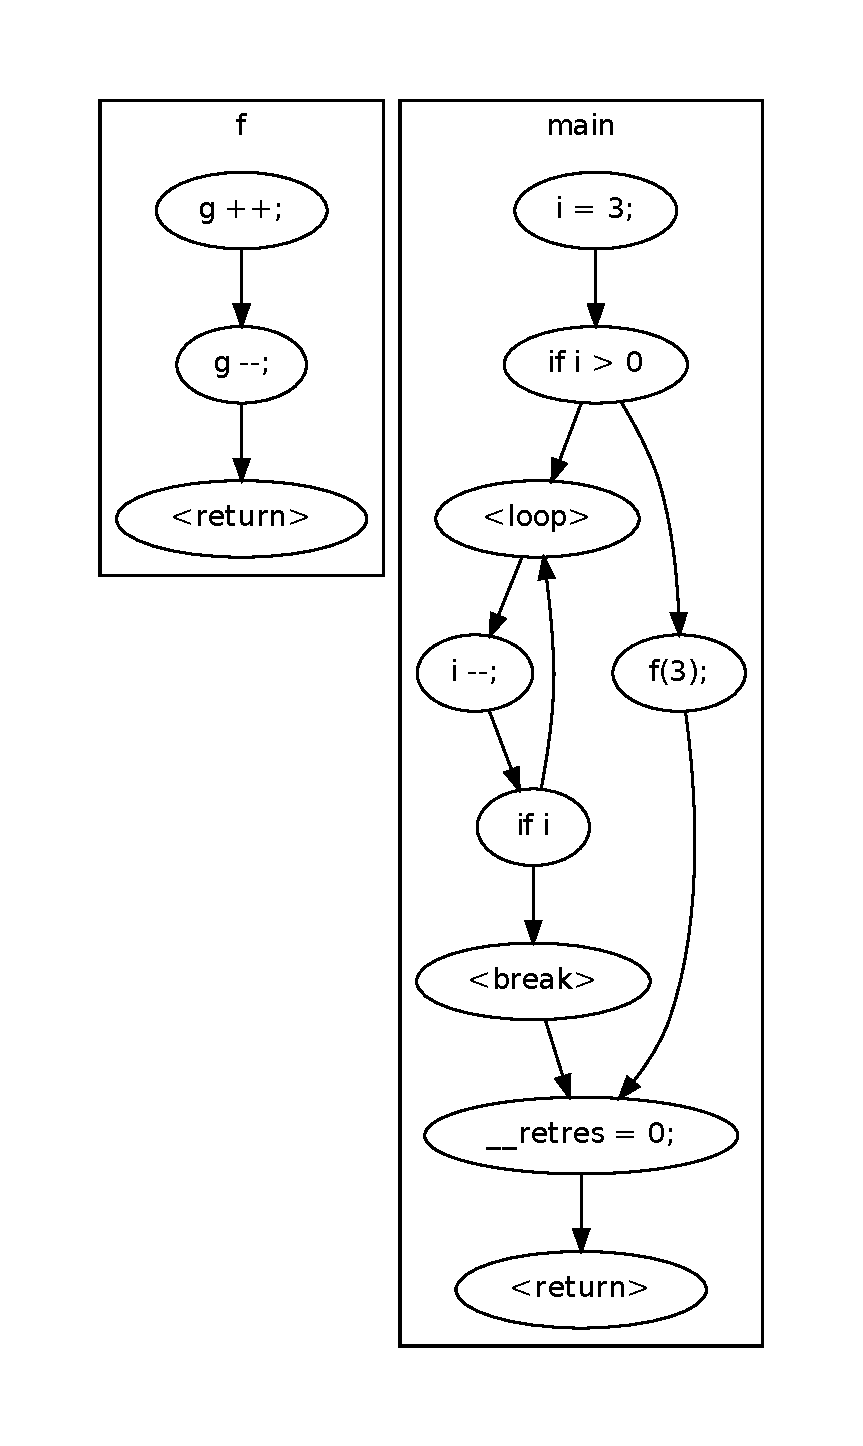
\includegraphics[width=\textwidth]{./tutorial/viewcfg/pdfs/cfg.pdf}
  \end{minipage}

  \caption{Control flow graph for file test.c.}
  \label{fig:tut:basiccfg}
\end{figure}

\subsubsection*{Further improvements}

There are many possible enhancements to this code:

\begin{itemize}
\item There is a bug when trying to print statements that contain
  strings (such as \verb|printf("Hello\n")| such statements must be
  protected using the \verb|"%S"| Format directive;
\item The script could be transformed into a regular plug-in, by
  registering into \framac, and taking options from the command line;
  for instance to compute the control flow graph of a single function
  given as an argument;
\item The graphs could be fancier, in particular by distinguishing
  between branching nodes and plain ones, or showing exit of blocks as
  well as their beginning; or linking a call with the called function.
\end{itemize}

We will concentrate on another extension, which is to reuse the
analysis of the \texttt{value} \framac plug-in to color unreachable
nodes.
To do so, because we will combine different plug-ins, we need to ensure their
correct ordering. This requires the definition of some command-line options.

\subsection{Plug-In registration and command-line options}\label{tut2:options}
\index{Plug-in!Command Line Options}\index{Command Line}

We have already seen how to register options in the previous ``Hello'' tutorial.
We now apply these principles to the ViewCfg plug-in.

\ocamlinput{./tutorial/viewcfg/src/register_and_options.ml}
\scodeidx{Plugin}{Register}
\ocamlinput{./tutorial/viewcfg/src/extend_with_run_with_options.ml}
\scodeidx{Visitor}{visitFramacFileSameGlobals}
\scodeidx{Ast}{get}

We added two options, \texttt{-cfg} to compute the CFG
conditionally (important for ordering plug-in executions),
and \texttt{-cfg-output} to choose the output file.

An interesting addition would be a \texttt{-cfg-target} option,
which would take a set of files or functions whose CFG would be
computed, using the \texttt{Self.Kernel\_function\_set} functor. Depending on
the targets, visiting the AST would have different starting points.
This is left as an exercise for the reader.

Another interesting exercise is to solve the following problem.
Currently, the complete CFG for the whole application is computed in
each \framac step, \ie executing \texttt{frama-c test.c -cfg
  -then -report} would compute the CFG twice. Indeed, the
\texttt{-cfg} option sets \texttt{Enabled} to true, and the
\texttt{run} function is executed once per task. To solve this
problem, one has to create a boolean state to remember that the plug-in
has already been executed. The \texttt{apply\_once} function in the
\texttt{State\_builder} module helps dealing with this issue (reading
the section~\ref{tut2:project-and-state} of this tutorial and
section~\ref{adv:project} of this manual should help you understand the
underlying notion of states).

With these command-line options, we can properly interface our ViewCfg plug-in
with the \texttt{value} plug-in.

\subsection{Interfacing with a kernel-integrated plug-in}

Kernel-integrated plug-ins, such as \texttt{value}, use a special mechanism
to statically register their APIs for other plug-ins that wish to access them.
This mechanism is the \texttt{Db} module of the \framac kernel,
the entry point for all kernel-integrated plug-ins. By using the functions
exported through the \texttt{Db.Value} module, our plug-in will obtain
reachability information computed by \texttt{value}.

The code modification we propose is to color in pink the nodes guaranteed to
be unreachable by the value analysis. For this purpose, we change the
\texttt{vstmt\_aux} method in the visitor:

\ocamlinput{./tutorial/viewcfg/src/print_cfg_vstmt_aux_value.ml}
\sscodeidx{Db}{Value}{is\_computed}
\sscodeidx{Db}{Value}{get\_stmt\_state}
\sscodeidx{Db}{Value}{is\_reachable}
\sscodeidx{Cil}{visitAction}{DoChildren}
\sscodeidx{Visitor}{frama\_c\_visitor}{vstmt\_aux}

This code fills the nodes with green if the node may be
reachable, and in pink if the node is guaranteed not to be
reachable; but only if the value analysis was previously computed. 

To test this code, frama-c should be launched with:
\begin{shell}
  frama-c test.c -load-script cfg_print.ml -val -then -cfg && dotty cfg.out
\end{shell}

Note that the relative order of the parameters \texttt{-load-script} and
\texttt{-val} in this example is not relevant
(see Section~\ref{adv:init} for details).
However, it is important to ensure that \texttt{-cfg} is separated from
\texttt{-val} by a \texttt{-then}; otherwise, it is not guaranteed that
the \texttt{value} plug-in will run before the ViewCfg plug-in, which might
lead to a non-colored graph in some cases, and colored in others.

The resulting graph is shown in Figure~\ref{fig:tut:coloredcfg}.

\begin{figure}[htbp]
  \centering
  \begin{minipage}[h]{0.45\linewidth}
  \listingname{test.c}
  \cinput{./tutorial/viewcfg/tests/test.c}
  \end{minipage}%
  \begin{minipage}[h]{0.4\linewidth}
    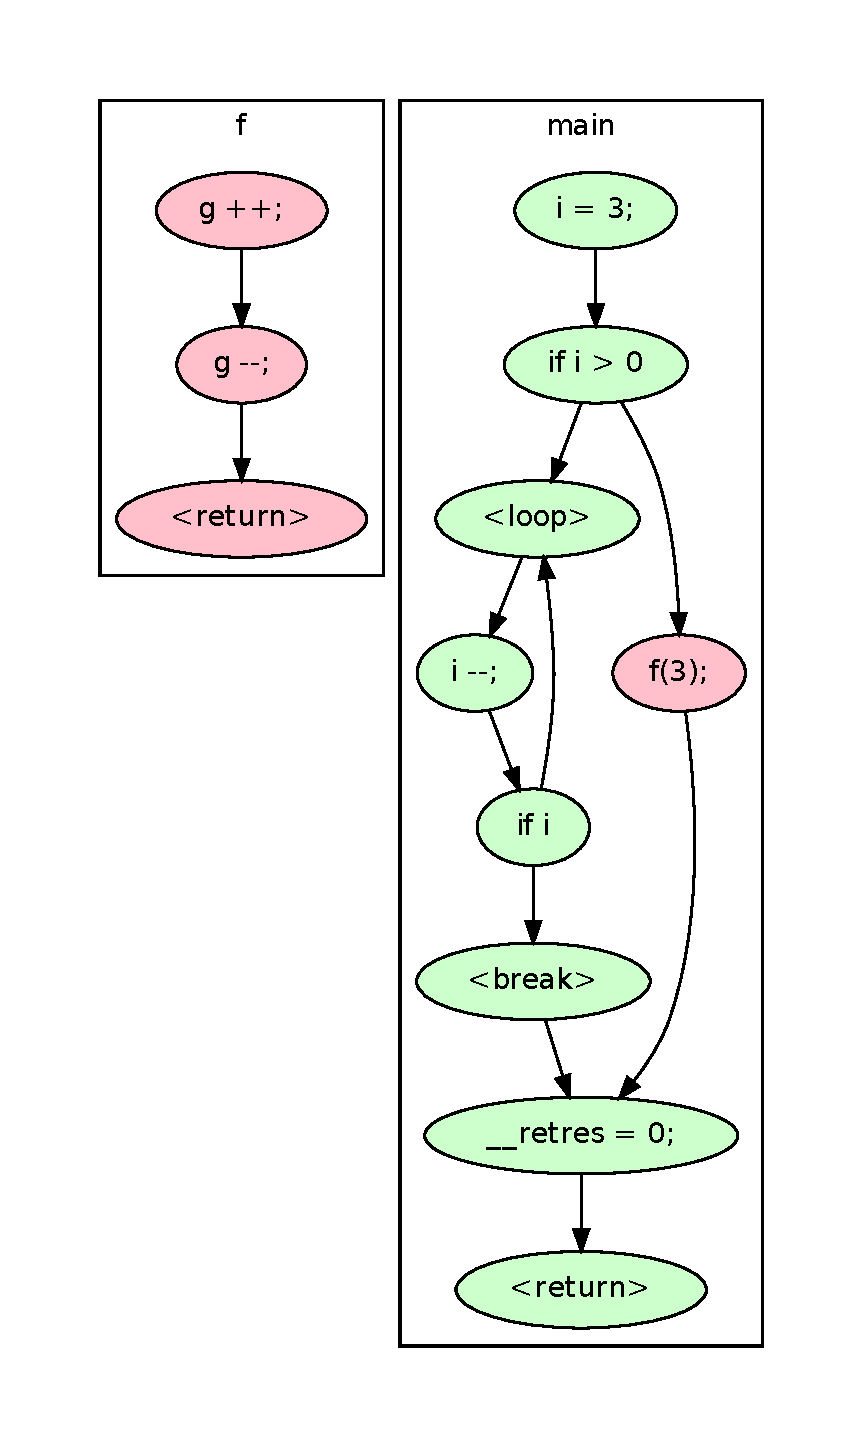
\includegraphics[width=\textwidth]{./tutorial/viewcfg/pdfs/cfg_colored.pdf}
  \end{minipage}
  \caption{Control flow graph colored with reachability information.}
  \label{fig:tut:coloredcfg}
\end{figure}

\subsection{Extending the Frama-C GUI}
\label{tut2:gui}
\index{Plug-in!GUI}

In this section, we will extend our plug-in so that the control flow
graph can be displayed interactively. For that, we will extend the \framac GUI
so that when you right-click on a function in the code, a new ``Show
CFG'' item appears, that displays the control flow graph of the
function in a dialog box. This is achieved just by appending the following
pieces of code at the end of the \texttt{cfg\_print.ml} file.

Currently, we used a visitor that outputs a \dottool file with the CFG of
all functions of all files. We use \texttt{dump\_function} to output
the CFG of a single function instead.

\ocamlinput{./tutorial/viewcfg/src/dump_function.ml}

We reused the \texttt{print\_cfg} visitor, but we selected a different
starting point. The argument \texttt{fundec} gets type
\texttt{Cil\_types.fundec}\scodeidx{Cil\_types}{fundec}, which is the CIL type
representing a function definition.

Now we write the GUI extension code:

\ocamlinput{./tutorial/viewcfg/src/gui.ml}
\scodeidx{Pretty\_source}{PVDecl}
\sscodeidx{Globals}{Functions}{get}
\scodeidx{Kernel\_function}{get\_definition}
\scodeidx{Gtk\_helper}{graph\_window}
\scodeidx{Design}{register\_extension}
\sscodeidx{Design}{main\_window\_extension\_points}{register\_source\_selector}

Let us explain this code from the end. \texttt{Design.register\_extension} is
the entry point for extending the GUI. Its argument is a function which takes as
argument an object corresponding to the main window of the \framac GUI. This
object provides access to the main widgets of the window, and several
extension points.

Here we have implemented a single extension, the ``source selector'',
that allows to add entries to menu obtained when right-clicking on the
source. This is implemented by the \texttt{cfg\_selector} function.

This function takes a \texttt{localizable} argument, which gives information on
where the user clicks on the source. Here we do something only if the user
clicks on the declaration of a variable whose type is a function (\ie when the
user clicked on a function declaration or definition).  In that case, we add an
item to the popup menu, that calls the \texttt{callback} function if
clicked. The \texttt{callback} function calls a \framac GUI function that
displays a graph from \dottool printing functions. It uses several important \framac
APIs: \texttt{Globals} and \texttt{Kernel\_function}, which contain several
functions for manipulating globals and functions.

Note that this GUI extension could also have been done through a script
(instead of a plug-in), but it would have been less than ideal.
In particular, the GUI \ocaml modules are available only when a script
is loaded with \texttt{frama-c-gui}, and not when loaded with
\texttt{frama-c}. When the user wants to view the CFG from the GUI,
outputting the CFG of all functions in \texttt{cfg.out} is useless.
A better architectural solution is to split our plug-in in several files,
with its own Makefile, to better manage its functionalities.

\subsection{Splitting files and writing a Makefile}\label{tut2:makefile}
\index{Plug-in!Makefile}

The \framac plug-in development environment allows to split GUI-related
and non-GUI related modules, so that GUI-related modules are loaded
and run only if \framac is executed with \texttt{frama-c-gui}. This
requires splitting the module into several files. We choose the
following architecture:

\begin{itemize}
\item \texttt{cfg\_options.ml} implements plug-in registration and
  configuration options;
\item \texttt{cfg\_core.ml} implements the main functions for
  computing the CFG;
\item \texttt{cfg\_register.ml} implements ``global'' computation of
  the CFG using the \texttt{-cfg} option, and hooking into the \framac
  main loop;
\item \texttt{cfg\_gui.ml} implements GUI registration.
\end{itemize}

Dependencies between the modules\footnote{This graphic is generated in
  file \texttt{doc/code/modules.dot} after running \texttt{make doc}.}
is presented on Figure \ref{fig:tut:cfgarchitecture}.

\begin{figure}[htbp]
  \centering
    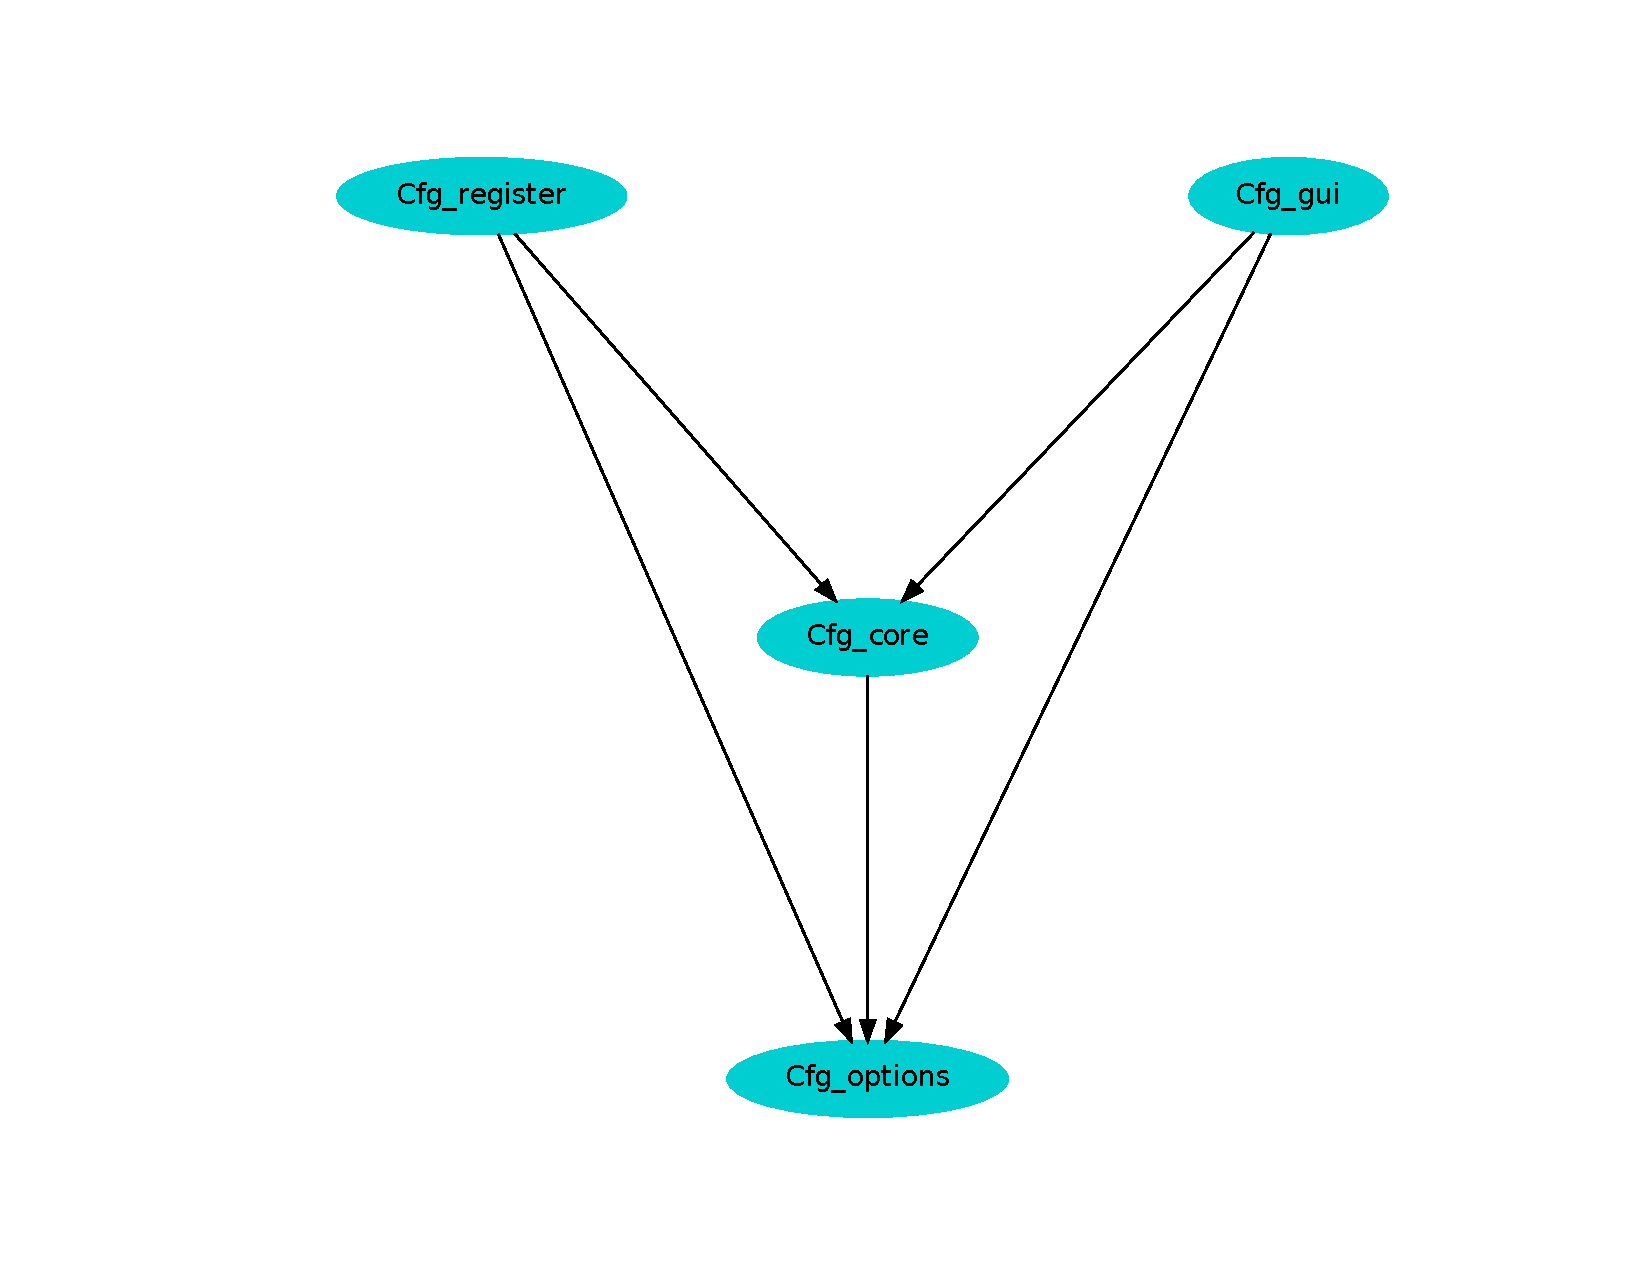
\includegraphics[width=0.5\textwidth]{./tutorial/viewcfg/pdfs/modules.pdf}
  \caption{CFG plug-in architecture}
  \label{fig:tut:cfgarchitecture}
\end{figure}

To break recursive dependencies between \ocaml modules, it is typical
that plug-in registration is done at the bottom of the module
hierarchy, while definition of the \texttt{run} function is at the
top. The GUI is also at the top of the hierarchy: the \framac
\texttt{Makefile} requires that normal plug-in modules do not depend on
GUI modules. Note that currently, the dependency from
\texttt{Cfg\_core} and \texttt{Cfg\_gui} to \texttt{Cfg\_register} is
artificial, but in future evolutions the GUI could depend on
configuration options.

\listingname{Makefile}
\codeidx{Makefile.dynamic}
\codeidx{FRAMAC\_SHARE}
\codeidx{PLUGIN\_CMO}
\codeidx{PLUGIN\_GUI\_CMO}
\codeidx{PLUGIN\_NAME}
\makefileinput{./tutorial/viewcfg/generated/split/Makefile}

In the \texttt{Makefile}, the \texttt{PLUGIN\_CMO} variable must
contain the list of file names of the ml files, in the correct \ocaml
build order. Modules in \texttt{PLUGIN\_CMO} must not depend on modules in
\texttt{PLUGIN\_GUI\_CMO}.

We also need to add an interface for the whole plug-in:
\listingname{ViewCfg.mli}
\ocamlinput{./tutorial/viewcfg/generated/split/ViewCfg.mli}

Here is the listing for the different modules:

\listingname{cfg\_options.ml}
\ocamlinput{./tutorial/viewcfg/generated/split/cfg_options.ml}

\listingname{cfg\_core.ml}
\ocamlinput{./tutorial/viewcfg/generated/split/cfg_core.ml}

\listingname{cfg\_register.ml}
\ocamlinput{./tutorial/viewcfg/generated/split/cfg_register.ml}

\listingname{cfg\_gui.ml}
\ocamlinput{./tutorial/viewcfg/generated/split/cfg_gui.ml}

\subsection{Getting your Plug-in Usable by Others}\label{tut2:api}
\index{Plug-in!API}
\todo

% TODO: A script that uses "dump_function" of the CFG plug-in

\subsection{Writing your Plug-in into the Journal}\label{tut2:journal}
\index{Journalization}
\todo

% TODO: Journalize dump_function.

% La journalisation, c'est le fait d'avoir la GUI rajouter des entrees
% dans le journal, pour pouvoir les rejouer. Ca permet, quand on
% paufine des analyses, de refaire ce qu'on a fait dans la gui
% automatiquement; apres on peut utiliser load-script pour rejouer le
% journal.

% Pour journaliser, il faut enregister la fonction pour qu'elle soit
% accessible de l'exterieur. Apres il y a un argument journalize qui
% permet de journaliser. Si je fais ca pour ma fonction dump_function,
% je vais recuperer une fonction dump_function_journalized; et c'est
% celle ci-qu'il faudrait que j'utilise dans la GUI; comme ca a chaque
% fois que je fais un "show-cfg", ce serait enregistre. La ce n'est
% pas tres interessant parce que je ne fais pas de modification de
% l'AST, mais dans le cas general ca l'est.

\subsection{Writing a Configure Script}\label{tut2:configure}
\index{Plug-in!Configure}
\todo

% Detect \dottool at compile time.
% Link to section 5.3: plug-in specific configure.in

\subsection{Getting your plug-in Usable in a Multi Projects Setting}
\label{tut2:project-and-state}
\index{Project}

\subsubsection{Registering and using state}

In this section, we will learn how to register state into \framac. A
\emph{state} is a piece of information kept by a plug-in. For instance,
the \texttt{value} plug-in computes, for each statement, a table associating to
each AST's variable a set of values the program may have at runtime: this
association table is a state.

State registration provides several features:
\begin{itemize}
\item It allows the state to be saved and reloaded with the rest of
  the session, for instance when using \texttt{frama-c -save/frama-c
    -load};
\item It helps maintaining consistency between the AST and the results and
  parameters of the analysis of the different plug-ins.
\end{itemize}

In this tutorial, we will store the file representing the \dottool
output of the control flow graph of a function (as needed by
\texttt{dump\_function}) as a string, by using a hashtable from \texttt{fundec}
to \texttt{string}. Storing this string will allow us to memoize~\cite{michie68}
our computation: the string is computed the first time the CFG of a
function is displayed, while the following requests will reuse the result of
the computation. Registering the hashtable as a \framac state is
\emph{mandatory} to ensure \framac consistency: for instance, by using a
standard \caml hashtable, a user that would have loaded several session through
the GUI could observe the CFG of function of a previous session instead of the
one he wants to observe.

Registering a state is done by a functor application:

\ocamlinput{./tutorial/viewcfg/src/register_cfg_graph_state.ml}
\scodeidx{State\_builder}{Hashtbl}
\sscodeidx{Cil\_datatype}{Fundec}{Hashtbl}
\scodeidx{Datatype}{String}
\scodeidx{Ast}{self}
\sscodeidx{Db}{Value}{self}

The \texttt{State\_builder} module provides several functors that help
registering states. \texttt{State\_builder.Hashtbl} allows the developer to
create a hashtable. It is parameterized by a module describing the hashtable
and its key, a module describing the data associated to keys, and
other informations. 

The \texttt{Datatype} and \texttt{Cil\_datatype} modules describe the
hashtable and its associated data, and explain for instance how the
datatype should be copied, printed, or marshalled to the disk. They
are part of the \texttt{Type} library~\cite{signoles:jfla11}, described in
Section~\ref{adv:datatype}. \texttt{Datatype} provides
descriptions for standard \caml types, and \texttt{Cil\_datatype} for
the CIL types (in the \texttt{Cil\_types} module).

The last module argument describes the initial size of the hashtable, a name
(mainly used for internal debugging), and a list of \emph{dependencies}. Here we
expressed that our hashtable depends on the Ast and the results of the
\texttt{Value} plug-in. For instance, whenever the \framac kernel updates one of these
states, it will automatically reset our hashtable. This ensures consistency of
the analysis: if the Ast of a function changes, or the value analysis is
executed with a different entry point, this potentially affects the display of
the control flow graph, that we must recompute.

Once the module has been declared, it is fairly easy to use it.

\ocamlinput{./tutorial/viewcfg/src/dump_to_string_memoized.ml}
\scodeidx{Visitor}{visitFramacFunction}
\ocamlinput{./tutorial/viewcfg/src/dump_function_memo_no_clear_cache.ml}

\texttt{dump\_function} now takes two steps: first the CFG is printed
to a string, then the string is printed to the \texttt{fmt}
argument. This allows the \texttt{dump\_to\_string} part to be
\emph{memoized}, \ie the results of \texttt{dump\_to\_string} are
saved so that later calls to \texttt{dump\_function} with the same
\texttt{fundec} argument reuse that result. 

If you launch \texttt{frama-c-gui} with the above code, click on
functions to view their CFG, and inspect the console, you will observe
that the string ``Computing CFG for function ...'' is displayed only
once per function.

One can see the effects of the dependency on the \texttt{Value} plug-in
by first launching the value analysis, inspecting the CFG for the
\texttt{f} function, then changing the entry point to \texttt{f} in the
CFG and re-running the value analysis. The console indicates that the
\texttt{CFG} have been recomputed. Indeed the state of the
\texttt{Value} plug-in, and of its dependencies, was reset when the
entry point was changed.

Another way to observe how \framac automatically handles states is to display a
CFG, save the session, close and restart \framac, 
and then reload the session: the control flow graph is not recomputed,
which means that \framac has automatically saved the
\texttt{Cfg\_graph\_state} with the rest of the session. Everything
should also work properly when loading several sessions.

\subsubsection{Clearing states, selection and projects}

There is one caveat though: if the user computes the CFG before
running the \texttt{Value} analysis, and then runs \texttt{Value}, he
will not see a colored graph (unless he re-launch the \texttt{Value}
analysis with different parameters). This is because the state of the
CFG is reset when the state of \texttt{Value} is reset, not when it is
first computed.

To solve this problem, we will manually reset the
\texttt{Cfg\_graph\_state} if we detect that the \texttt{Value}
analysis has been run since the last time we computed the CFG. For
that, we have to remember the previous value of
\texttt{Db.Value.is\_computed ()}, \ie to register another state:

\ocamlinput{./tutorial/viewcfg/src/register_value_computed_state.ml}
\scodeidx{State\_builder}{Ref}
\scodeidx{Datatype}{Bool}

This new state only consists of a reference to a boolean value.

Then we just replace \texttt{dump\_function} in the code above by the
following.

\ocamlinput{./tutorial/viewcfg/src/dump_function_memo_clear_cache.ml}
\sscodeidx{Db}{Value}{is\_computed}
\scodeidx{State\_selection}{with\_dependencies}
\scodeidx{Project}{clear}

The only part that need to be explained is the notion of
\emph{selection} and \emph{project}. A selection is just a set of
states; here we selected the state \texttt{Cfg\_graph\_state} with all
its dependencies, as resetting this state would also impact states
that would depend on it (even if there is none for now). We use
\texttt{Project.clear} to reset the selection.

\subsubsection{Project explanation}

A \emph{project}~\cite{project} is a consistent version of all the \emph{states}
of \framac. \framac is multi-AST, \ie \framac plug-ins can change the AST of the
program, or perform incompatible analysis (\eg with different entry
points). Projects consistently groups a version of the AST of the program, with
the states related to this AST.

The \texttt{Project.clear} function has type :
\begin{ocamlcode}
val clear: ?selection:State_selection.t -> ?project:t -> unit -> unit  
\end{ocamlcode}
\scodeidxdef{Project}{clear}
\scodeidx{State\_selection}{t}
\scodeidx{Project}{t}

The arguments \texttt{selection} and \texttt{project} can be seen as a
coordinate system, and the function allows to clear specific versions
of specific states. By default, \framac functions act on the
\emph{current} project. The developer has to use \texttt{Project.on} or optional
arguments to act on different projects. \framac automatically handles
duplication and switch of states when duplicating or changing of
projects. This is the last benefit of state registration.

To summarize:

\begin{itemize}
\item To store results, plug-ins should register \emph{states};
\item A \emph{project} is a consistent version of all the states in
  \framac, together with a version of the AST;
\item A \emph{session} is a set of \emph{projects};
\item \framac transparently handles the versioning of states when
  changing or duplicating projects, saving and reloading sessions from
  disk, etc.
\item The version of the state in a project can change; by default
  \framac functions operate on the current project.
\item A \emph{selection} is a set of states. \emph{Dependencies} allow
  to create selections.
\item As a plug-in developer, you have to remember that is up to you to preserve
  consistency between your states and their dependencies by clearing the latter
  when the former is modified in an incompatible way. For instance, it would
  have been incorrect to not call 
  \texttt{State\_selection.with\_dependencies}
  \scodeidx{State\_selection}{with\_dependencies} in the last code snippet of
  this tutorial.
\end{itemize}

Projects are generally created using copy visitors. We encourage the reader to
experiment with multiple projects development by using them. An interesting
exercise would be to change the AST so that execution of each instruction is
logged to a file, and then re-read that file to print in the CFG how much time
each instruction has been executed. Another interesting exercise would be
to use the \texttt{apply\_once} function so that the ViewCfg plug-in is executed
only once, as explained in section~\ref{tut2:options} of this tutorial.

%; whizzy-master "developpeur.tex"

\chapter{Software Architecture}\label{chap:archi}\index{Architecture}

\begin{target}beginners.\end{target}

In this chapter, we present the software architecture of \framac. First,
Section~\ref{archi:general} presents its general overview. Then, we focus on
four different parts:

\begin{itemize}
\item Section~\ref{archi:plugin} explains what a plug-in really is and the main
  mechanisms of plug-in integration.
\item Section~\ref{archi:libraries} introduces the libraries that \framac
  provides.
\item Section~\ref{archi:services} introduces the kernel services that plug-in
  developers might want to use.
\item Section~\ref{archi:internals} introduces the kernel internals. You can
  safely skip it if you are not a \framac kernel developer.
\end{itemize}

%%%%%%%%%%%%%%%%%%%%%%%%%%%%%%%%%%%%%%%%%%%%%%%%%%%%%%%%%%%%%%%%%%%%%%%%%%%%%%%

\section{General Description}\label{archi:general}

From a plug-in developer point of view, the main goals of the \framac platform
is to provide services to ease:
\begin{itemize}
\item analysis and source-to-source transformation of big-size \C programs;
\item addition of new plug-ins; and
\item plug-ins collaboration.
\end{itemize}

In order to reach these goals, \framac has a plug-ins based software
architecture based on a \emph{kernel}\index{Kernel}. Historically the
\emph{kernel} was itself based on \cil~\cite{cil}: even if they have evolved
separately since the \framac Hydrogen age, there are still a lot of similarities
between \cil and several modules of the \framac kernel (\eg the ASTs).

The \framac architecture design is presented in this chapter, and summarized in
Figure~\ref{fig:architecture}. In this figure, each of the four rounded colored
boxes represents a subdirectory $d$ of directory \texttt{src}, while each of the
small square boxes represents a subdirectory in one subdirectory
\texttt{src/$d$}. The remaining sections will explain the goal of each of these
boxes. They do not detail each module of each directory: use the API
documentation generated by \texttt{make doc} for that purpose.

\begin{figure}[htbp]
\begin{center}

\begin{tikzpicture}[remember picture,every node/.style={transform shape}]
\node (bottom) {
\begin{tikz-hbox}[node distance=\bigpadding]{bottom}
% kernel internals
\node[structural,on chain] (internals) {
  \tikztitleboxbig{Kernel Internals}{LightCyan}{
    \begin{tikz-hbox}{internals}
      \node[on chain,draw,plain]{parsing};
      \node[on chain,draw,plain]{typing};
      \node[on chain,draw,plain]{runtime};
    \end{tikz-hbox}
  }
};

% libraries
\node[structural, on chain] (libraries) {%
  \tikztitleboxbig{Libraries}{Orange}{
    \begin{tikz-vbox}[node distance=\bigpadding]{libraries}
      \node[on chain,draw,plain] (stdlib){stdlib};
      \node[on chain,structural]{
        \begin{tikz-hbox}{lib-middle}
          \node[on chain,draw,plain] (datatype) {datatype};
          \node[on chain,draw,plain] (project) {project};
        \end{tikz-hbox}
      };
      \node[on chain,draw,plain] (utils) {utils};
    \end{tikz-vbox}%
  }
};
\end{tikz-hbox}
\begin{tikzpicture}[overlay]
    \draw[Latex-Latex] (stdlib.south) -- (datatype);
    \draw[Latex-Latex] (datatype) -- (utils);
    \draw[-Latex] (project) -- (stdlib);
    \draw[-Latex] (project.west) -- (datatype.east);
    \draw[-Latex] (project) -- (utils);
    \draw[-Latex,looseness=1.7,in=-20,out=20] (utils.east) to (stdlib.east);
\end{tikzpicture}
};

\node[structural, above=\bigpadding] at (bottom.north) (services) {
    % kernel services
  \tikztitleboxbig{Kernel Services}{darkgreen}{
    \begin{tikz-hbox}{services}
      \node[on chain,structural]{
        \begin{tikz-vbox}{services-left}
          \node[on chain,structural] (traversal){
            \tikztitlebox{AST Traversal}{%
              \begin{tikz-vbox}{traversal}
                \node[on chain,draw,plain] (visitor) {visitor};
                \node[on chain,structural] {
                  \begin{tikz-hbox}{traversal-1}
                    \node[on chain,draw,plain] (analysis) {analysis};
                    \node[on chain,draw,plain] (transfo) {ast\_transformations};
                  \end{tikz-hbox}
                };
                \draw[-Latex] (analysis) -- (visitor);
                \draw[-Latex] (transfo) -- (visitor);
              \end{tikz-vbox}
            }
          };
          \node[on chain,structural] (ai) {
            \tikztitlebox{AI}{
              \begin{tikz-vbox}{ai}
                \node[on chain,draw,plain]      {abstract\_interp};
              \end{tikz-vbox}
            }
          };
        \end{tikz-vbox}
      };
      \node[on chain,structural]  {
        \begin{tikz-vbox}{services-right}
          \node[on chain,structural](ast){
            \tikztitlebox{ASTs}{%
              \begin{tikz-vbox}{ast}
                \node[on chain,draw,plain] (data) {ast\_data};
                \node[on chain,draw,plain] (queries) {ast\_queries};
                \node[on chain,draw,plain] (parsetree) {parsetree};
                \draw[-Latex] (queries) -- (data);
              \end{tikz-vbox}
            }
          };
          \node[on chain,structural] (interactions) {
            \tikztitlebox{Plug-in Interactions}{
              \begin{tikz-vbox}{plugin-api}
                \node[on chain,draw,plain] {cmdline\_parameters};
                \node[on chain,draw,plain] {plugin\_entry\_points};
              \end{tikz-vbox}
            }
          };
          \draw[bigarrow,<->] (ast.south) -- (interactions.north);
        \end{tikz-vbox}
      };
    \end{tikz-hbox}
    \begin{tikzpicture}[overlay]
      \coordinate (ai2) at ($(ai.north east)!.75!(ai.south east)$);
      \coordinate (traversal1) at
      ($(traversal.south east)!0.2!(traversal.south west)$);
      \coordinate (interactions1) at
      ($(interactions.north west)!0.2!(interactions.south west)$);
      \draw[bigarrow,->] (traversal.east) -- (ast.west);
      \draw[bigarrow,->] (traversal1) -- (interactions1);
      \draw[bigarrow,bend right, ->] (ai.east) to[in=170] (ast.west);
      \draw[bigarrow,->] (ai.east) -- (interactions.west);
    \end{tikzpicture}
  }
};

%plugins
\node[above=\bigpadding,structural] at (services.north) (plugins) {
  \tikztitleboxbig{Plug-ins}{palered}{
    \begin{tikz-hbox}{plugins}
      \node[on chain,draw,plain] (pi1) {plug-in 1};
      \node[on chain,draw,plain] (pi2) {plug-in 2};
      \node[on chain,plain,minimum height=1ex] (dots) {...};
      \node[on chain,draw,plain] (pin) {plug-in $n$};
      \draw[-Latex,bend left] (pi1.north) to (pi2.north);
      \draw[-Latex,bend left] (pi2.north) to (dots.north);
      \draw[-Latex,bend left] (dots.north) to (pin.north);
      \draw[-Latex,bend left] (pin.south) to (dots.south);
      \draw[-Latex,bend left] (dots.south) to (pi2.south);
      \draw[-Latex,bend left] (pi2.south) to (pi1.south);
    \end{tikz-hbox}
  }
};

   \draw[bigarrow,<->] (services.south) -- (internals.north);
   \draw[bigarrow,->] (plugins.south) -- (services.north);
   \draw[bigarrow,->] (internals.east) -- (libraries.west);
   \draw[bigarrow,->] (services.south) to (libraries.north);
\end{tikzpicture}
\caption{Frama-C Architecture Design.}\label{fig:architecture}
\end{center}
\end{figure}

%%%%%%%%%%%%%%%%%%%%%%%%%%%%%%%%%%%%%%%%%%%%%%%%%%%%%%%%%%%%%%%%%%%%%%%%%%%%%%%

\section{Plug-ins}\label{archi:plugin}
\index{Plug-in}\index{Plug-in!Kernel-integrated}

In \framac, plug-ins are program analysis or source-to-source
transformations. The ones provided within \framac are in directory
\texttt{src/plugins/$plugin\_name$}. Each plug-in is an extension point of \framac which
has to be registered through \texttt{Plugin.Register}\scodeidx{Plugin}{Register}
(see Section~\ref{adv:plugin-services}). \framac allows plug-in collaborations:
a plug-in $p$ can use a list of plug-ins $p_1$, \dots, $p_n$ and
conversely. Mutual dependences between plug-ins are even possible. If a plug-in
is designed to be used by another plug-in, it has to register its API either by
providing a \texttt{.mli} file, or through modules
\texttt{Dynamic}\codeidx{Dynamic} or \texttt{Db}\codeidx{Db}. The first method
is the preferred one, the second one (through module \texttt{Dynamic}) is the
only possible one to define mutually dependent plug-ins while the third one
(through module \texttt{Db}) is now fully deprecated even if most of the older
\framac plug-ins are still defined this way.

%%%%%%%%%%%%%%%%%%%%%%%%%%%%%%%%%%%%%%%%%%%%%%%%%%%%%%%%%%%%%%%%%%%%%%%%%%%%%%%

\section{Libraries}\label{archi:libraries}

Libraries are defined in the directory \texttt{src/libraries}. They are either
third-party libraries or dedicated independent libraries which may be used by
other parts of \framac.

Extension of the \caml standard library are provided in directory
\texttt{src/libraries/stdlib}. For instance, modules \texttt{FC$module\_name$}
(e.g. \texttt{FCHashtbl}\codeidxdef{FCHashtbl}) provides a
\texttt{$module\_name$}-like interface (e.g. \texttt{Hashtbl}) with an uniform
API for all \ocaml versions supported by \framac and possibly additional useful
operations for the corresponding datastructures.

Single-file libraries are provided in directory
\texttt{src/libraries/utils}. For instance,
\texttt{Pretty\_utils}\codeidxdef{Pretty\_utils} provides pretty-printing
facilities.

\emph{datatype} (directory \texttt{src/libraries/datatype}) and \emph{project}
(directory \texttt{src/libraries/project}) are two multiple-files
libraries. They are respectively presented in Sections~\ref{adv:datatype} and
\ref{adv:project}.

%%%%%%%%%%%%%%%%%%%%%%%%%%%%%%%%%%%%%%%%%%%%%%%%%%%%%%%%%%%%%%%%%%%%%%%%%%%%%%%

\section{Kernel Services}\label{archi:services}\index{Kernel!Services|bfit}

The kernel services is defined in directory \texttt{src/kernel\_services}. It
is the part of the \framac kernel which may be useful to develop plug-ins.

This services may be split in four main parts:
\begin{itemize}
\item two ASTs and the data structures directly built upon them;
\item plug-in interactions toolbox;
\item predefined generic analyzers;
\item the abstract interpretation framework.
\end{itemize}

The standard AST used by most analyzers is defined in module
\texttt{Cil\_types}\codeidx{Cil\_types} of directory
\texttt{src/kernel\_services/ast\_data}. It contains the types which describes
both the \C constructs and the \acsl ones~\cite{acsl}. The same directory also
contains modules defining datastructures directly based upon the AST (module
\texttt{Globals}\codeidx{Globals}), functions (module
\texttt{Kernel\_function}\codeidx{Kernel\_function}), annotations (module
\texttt{Annotations}\codeidx{Annotations}) and so on. A related directory is
\texttt{src/kernel\_services/ast\_queries}. It contains modules which provides
specific operations in order to get information about AST-related values.

In the same way, an untyped AST quite close of the \C input source is defined in
module \texttt{Cabs}\codeidx{Cabs} of directory
\texttt{src/kernel\_services/parsetree}. This AST is only well suited
for syntactic analyzers/program transformers.

\framac also provides services to plug-ins which help both their integration in
the platform and their interactions with the kernel and the other plug-ins. They
enforce some platform-wide consistency by ensuring that some common actions
(\emph{e.g.} printing messages to end-users) are handled by all plugins in a
similar way. Directory \texttt{src/kernel\_services/cmdline\_parameters}
provides modules which eases the definition of analyzers' parameters accessible
by the end-user through command-line options. Similarly, directory
\texttt{src/kernel\_services/plugin\_entry\_points} provides modules to interact
with the \framac kernel or other plug-ins.

Next, \framac provides predefined ways to visit the ASTs, in particular through
object-oriented visitors defined in directory
\texttt{src/kernel\_services/visitors} (see Section~\ref{adv:visitors}). 
Some predefined analyzers, such as a multiple generic dataflow analysis
are provided in directory \texttt{src/kernel\_services/analysis}, while some
predefined program transformation, such as cloning a function, are provided in
directory \texttt{src/kernel\_services/ast\_transformations}.
Finally, \framac provides an abstract interpretation 
toolbox\index{Abstract Interpretation}
with various lattices in directory \texttt{abstract\_interp}.

%%%%%%%%%%%%%%%%%%%%%%%%%%%%%%%%%%%%%%%%%%%%%%%%%%%%%%%%%%%%%%%%%%%%%%%%%%%%%%%

\section{Kernel Internals}\label{archi:internals}\index{Kernel!Internals|bfit}

\begin{target}kernel developers.\end{target}

The kernel internals is defined in directory \texttt{src/kernel\_internals}. It
is part of the \framac kernel which should be useless to develop analysis
plug-ins, except possibly for very low-level interactions, or to extend the
C or ACSL services of Frama-C. Consequently, if you are not a kernel
developer, you can safely ignore this section.

The internals is split in three different parts, each of them being an
independent subdirectory:
\begin{itemize}
\item the directory \texttt{src/kernel\_internals/parsing} contains the lexer
  and parser which generate the untyped AST (\emph{aka} Cabs) from the \C input
  source code;
\item the directory \texttt{src/kernel\_internals/typing} contains the
  compiler which generates the standard AST (\emph{aka} Cil) from the untyped
  one;
\item the directory \texttt{src/kernel\_internals/runtime} contains modules
  whose primary purpose is to perform side-effects while \framac is booting.
\end{itemize}

% Local Variables:
% TeX-master: "developer.tex"
% ispell-local-dictionary: "english"
% End:

%%% Local Variables:
%%% TeX-master: "developer.tex"
%%% ispell-local-dictionary: "english"
%%% End:

\chapter{Advanced Plug-in Development}\label{chap:advance}
\lstset{language=Ocaml} %% makes Ocaml the default language for listings, eg. \lstinline.

This chapter details how to use services provided by \framac in order to be
fully operational with the development of plug-ins. Each section describes
technical points a developer should be aware of. Otherwise,
one could find oneself in one or more of the following situations
\footnote{It
  is fortunately quite difficult (but not impossible) to fall into the worst
  situation by mistake if you are not a kernel developer.}
(from bad to worse):
\begin{enumerate}
\item reinventing the (\framac) wheel;
\item being unable to do some specific things (\eg saving
  results\index{Saving} of an analysis on disk, see
  Section~\ref{proj:states});
\item introducing bugs in his/her code;
\item introducing bugs in other plug-ins using his/her code;
\item breaking the kernel consistency\index{Consistency} and so potentially
  breaking all \framac plug-ins (\eg if s/he modifies the
  AST\index{AST!Modification} without changing project\index{Project}, see
  Section~\ref{proj:use}).
\end{enumerate}

In this chapter, we suppose that the reader is able to write a minimal plug-in
like \texttt{hello}\index{Hello} described in chapter~\ref{chap:tutorial} and
knows about the software architecture of \framac (chapter~\ref{chap:archi}). Moreover
plug-in development requires the use of advanced features of
\caml (module system, classes and objects, \emph{etc}). Static plug-in
development requires some knowledge of \autoconf and \make.
 Each section summarizes its own prerequisites at its beginning (if any).

Note that the following subsections can be read in no particular
order: their contents are indeed quite independent from one another even if
there are references from one chapter to another one. Pointers to
reference manuals (Chapter~\ref{chap:refman}) are also provided for readers who
want full details about specific parts.

%%%%%%%%%%%%%%%%%%%%%%%%%%%%%%%%%%%%%%%%%%%%%%%%%%%%%%%%%%%%%%%%%%%%%%%%%%%%%%%

%% \section{File Tree Overview}\label{adv:files}

%% \begin{target}beginners.\end{target}

%% The \framac main directory is split in several sub-directories. The \framac source
%% code is mostly provided in directories \texttt{cil}\codeidx{cil} and
%% \texttt{src}\codeidx{src}. The first one contains the source code of
%% \cil~\cite{cil}\index{Cil} extended with an \acsl~\cite{acsl}
%% implementation\index{ACSL}. The second one is the core implementation of
%% \framac. This last directory contains directories of the \framac
%% kernel\index{Kernel} and directories of the provided \framac plug-in.

%% A pretty complete description of the \framac file tree is provided in
%% Section~\ref{refman:files}.

%%%%%%%%%%%%%%%%%%%%%%%%%%%%%%%%%%%%%%%%%%%%%%%%%%%%%%%%%%%%%%%%%%%%%%%%%%%%%%%

\section{\framac Configure.in}\label{adv:configure}
\codeidxdef{configure.in}

\begin{target}not for standard plug-ins developers.\end{target}

\begin{prereq}
  Knowledge of \autoconf and shell programming.
\end{prereq}

In this Section, we detail how to modify the file \texttt{configure.in} in
order to configure plug-ins (\framac configuration has been introduced in
Section~\ref{tut2:configure} and~\ref{tut2:makefile}).

First Section~\ref{conf:principle} introduces the general principle and
organisation of \texttt{configure.in}. Then Section~\ref{conf:add} explains how
to configure a new simple plug-in without any dependency. Next we show how to
exhibit dependencies with external libraries and tools
(Section~\ref{conf:dep-lib}) and with other plug-ins
(Section~\ref{conf:dep-plug}). Finally Section~\ref{conf:lib} presents the
configuration of external libraries and tools needed by a new plug-in but not
used anywhere else in \framac.

\subsection{Principle}\label{conf:principle}

When you execute \texttt{autoconf}, file \texttt{configure.in} is used to
generate the \texttt{configure} script. Each \framac user executes this script
to check his/her system and determine the most appropriate configuration: at the
end of this configuration (if successful), the script summarizes the
status of each plug-in, which can be:\index{Plug-in!Status}
\begin{itemize}
\item \emph{available} (everything is fine with this plug-in);
\item \emph{partially available}: either an optional dependency of the plug-in
  is not fully available, or a mandatory dependency of the plug-in is only
  partially available; or\index{Plug-in!Dependency}
\item \emph{not available}: either the plug-in itself is not provided by
  default, or a mandatory dependency of the plug-in is not available.
\end{itemize}

The important notion in the above definitions is
\emph{dependency}\index{Plug-in!Dependency|bfit}. A dependency of a plug-in $p$
is either an external library/tool\index{Library}\index{Tool} or another
\framac plug-in. It is either \emph{mandatory} or \emph{optional}. A mandatory
dependency must be present in order to build $p$, whereas an optional
dependency provides features to $p$ that are additional but not highly required
(especially $p$ must be compilable without any optional dependency).

Hence, for the plug-in developer, the main role of \texttt{configure.in} is to
define the optional and mandatory dependencies of each plug-in. Another standard
job of \texttt{configure.in} is the addition of options \texttt{---enable-$p$}
and \texttt{---disable-$p$} to \texttt{configure} for a plug-in $p$. These
options respectively forces $p$ to be available and disables $p$ (its status is
automatically ``not available'').

Indeed \texttt{configure.in} is organised in different sections specialized in
different configuration checks. Each of them begins with a title delimited by
comments and it is highlighted when \texttt{configure} is executed. These
sections are described in Section~\ref{refman:configure}. Now we focus on
the modifications to perform in order to integrate a new plug-in in \framac.

\subsection{Addition of a Simple Plug-in}\label{conf:add}

In order to add a new plug-in, you have to add a new subsection for the new
plug-in to Section \emph{Plug-in wished}. This action is usually very easy to
perform by copying/pasting from another existing plug-in (\eg
\texttt{occurrence}\index{Plug-in!Occurrence|see{Occurrence}}\index{Occurrence})
and by replacing the plug-in name (here \texttt{occurrence}) by the new plug-in
name in the pasted part. In these sections, plug-ins are sorted according to a
lexicographic ordering.

For instance, Section \emph{Wished Plug-in} introduces a new sub-section for
the plug-in \texttt{occurrence} in the following way.
\codeidxdef{check\_plugin}
\begin{configurecode}
# occurrence
############
check_plugin(occurrence,src/plugins/occurrence,
             [support for occurrence analysis],yes)
\end{configurecode}
\begin{itemize}
\item The first argument is the plug-in name,
\item the second one is the name of directory containing the source files 
  of the plug-in (usually a sub-directory of \texttt{src/plugins}), 
\item the third one is an help message for the \texttt{--enable-occurrence} 
  option of \texttt{configure},
\item the last one indicates if the plug-in is enabled by default
  (\texttt{yes/no}).
\end{itemize}

\begin{important}
The plug-in name must contain only alphanumeric characters and
underscores. It must be the same as the \texttt{name} value given as
argument to the functor \texttt{Plugin.Register} of
section~\ref{adv:plugin-services} (with spaces replaced by underscore). It must
also be the same (modulo upper/lower case) as the \texttt{PLUGIN\_NAME} variable
given in the plugin's Makefile presented in section~\ref{adv:dynamic-make}.
\end{important}

\begin{important}
  The macro \texttt{check\_plugin}\scodeidx{configure.in}{check\_plugin} sets
  the following variables:
  \texttt{FORCE\_OCCURRENCE}\scodeidxdef{configure.in}{FORCE\_$plugin$},
  \texttt{REQUIRE\_OCCURRENCE}\scodeidx{configure.in}{REQUIRE\_$plugin$},
  \texttt{USE\_OCCURRENCE}\scodeidx{configure.in}{USE\_$plugin$}, and
  \texttt{ENABLE\_OCCURRENCE}\scodeidxdef{configure.in}{ENABLE\_$plugin$}.
\end{important}

The first variable indicates if the user explicitly requires the availability of
\texttt{occurrence} \emph{via} setting the option
\texttt{---enable-occurrence}. The second and third variables are used by others
plug-ins in order to handle their dependencies (see
Section~\ref{conf:dep-plug}). The fourth variable \texttt{ENABLE\_OCCURRENCE} indicates
the plug-in status (available, partially available or not available). 
%At the end of these lines of code, it says if the plug-in should be compiled: if
If \texttt{---enable-occurrence} is set, then \texttt{ENABLE\_OCCURRENCE} is \yes
(plug-in available); if \texttt{---disable-occurrence} is set, then its value is
\texttt{no} (plug-in not available). If no option is specified on the command
line of \texttt{configure}, its value is set to the default one (according to
%\texttt{\$default}). 
the value of the fourth argument of \texttt{check\_plugin}).

%%%%
\subsection{Configuration of New Libraries or Tools}
\label{conf:lib}
\index{Library!Configuration}
\index{Tool!Configuration}

Some plug-ins need additional tools or libraries to be fully
functional. The \texttt{configure} script takes care of these in two
steps. First, it checks that an appropriate version of each external
dependency exists on the system. Second, it verifies for each plug-in
that its dependencies are met. Section~\ref{conf:dep-lib} explains how
to make a plug-in depend on a given library (or tool). The present
section deals with the first part, that is how to check for a given
library or tool on a system. Configuration of new libraries and configuration of
new tools are similar.  In this section, we therefore choose to focus
on the configuration of new libraries. This is done by calling a
predefined macro called
\texttt{configure\_library}\scodeidxdef{configure.in}{configure\_library}\scodeidxdef{configure.in}{configure\_tools}\footnote{For
  tools, there is a macro \texttt{configure\_tool} which works in the
  same way as \texttt{configure\_library}.}, or its more specialized version
\texttt{configure\_pkg}\scodeidxdef{configure.in}{configure\_pkg}.

\texttt{configure\_pkg} is meant to be used for checking the presence of
OCaml libraries that are managed as
\texttt{findlib}\footnote{\url{http://projects.camlcity.org/projects/findlib.html}}
packages, which is the case for most modern OCaml libraries nowadays.
It takes two arguments, the name of the package (as known by \texttt{findlib}),
and a message that will be displayed if the package is not found.

The \texttt{configure\_library} macro takes three arguments. The first one is
the name of the library, the second one is a filename
which is used by the script to check the availability of the library.
In case there are multiple locations possible for the library, this
argument can be a list of filenames. In this case, the argument must
be properly quoted ({\it i.e.} enclosed in a {\tt [}, {\tt]} pair).
Each name is checked in turn. The first one which corresponds to an
existing file is selected.  If no name in the list corresponds to an
existing file, the library is considered to be unavailable. The last
argument is a warning message to display if a configuration problem
appears (usually because the library does not exist). Using these
arguments, the script checks the availability of the library.

Results of these macros are available through variables which are
substituted in the files generated by \texttt{configure}, where
\texttt{$library$} stands for the \emph{uppercased}
version of the library name.
\begin{itemize}
\item For \texttt{configure\_pkg}:
\begin{itemize}
\item \texttt{HAS\_OCAML\_$library$}
\scodeidxdef{configure.in}{HAS\_OCAML\_$library$}
is set to \texttt{yes} or \texttt{no} depending on the availability
of the library
\end{itemize}
\item For \texttt{configure\_library}:
\begin{itemize}
\item \texttt{HAS\_$library$}\scodeidxdef{configure.in}{HAS\_$library$}
  is set to \texttt{yes} or \texttt{no} depending on the availability
  of the library
\item \texttt{SELECTED\_$library$}\scodeidxdef{configure.in}{SELECTED\_$library$}
contains the name of the version selected as described above.
\end{itemize}
\end{itemize}

If checking for \ocaml{} libraries and object files without
\texttt{configure\_pkg}, remember that
they come in two flavors: bytecode and native
code, which have distinct suffixes. Therefore, you should use the
variables \texttt{LIB\_SUFFIX}\scodeidx{configure.in}{LIB\_SUFFIX}
(for libraries) and
\texttt{OBJ\_SUFFIX}\scodeidx{configure.in}{OBJ\_SUFFIX}
(for object files) to check the presence of a
given file. These variables are initialized at the beginning of the
\texttt{configure} script depending on the availability of a
native-code compiler on the current installation.

\begin{example}
  The library \lablgtksourceview\index{Lablgtksourceview2} (used to have a
  better rendering of C sources in the GUI) is part of
  \lablgtk\index{Lablgtk}~\cite{lablgtk}.
  This is checked through the following command,
  where \texttt{LABLGTKPATH\_FOR\_CONFIGURE} is the path where
  \texttt{configure} has found \lablgtk itself.

\begin{configurecode}
configure_library(
  [GTKSOURCEVIEW],
  [\$LABLGTKPATH_FOR_CONFIGURE/lablgtksourceview2.\$LIB_SUFFIX],
  [lablgtksourceview not found])
\end{configurecode}
\end{example}

\subsection{Addition of Library/Tool Dependencies}\label{conf:dep-lib}
\index{Library!Dependency}\index{Tool!Dependency}

Dependencies upon OCaml packages (checked by \texttt{configure\_pkg}) are
governed by two macros:

\begin{itemize}
\item \texttt{plugin\_require\_pkg($plugin$,$library$)}%
\scodeidxdef{configure.in}{plugin\_require\_pkg} indicates that
$plugin$ requires $library$ in order to be compiled.
\item \texttt{plugin\_use\_pkg($plugin$,$library$)}%
\scodeidxdef{configure.in}{plugin\_use\_pkg} indicates that
$plugin$ uses $library$, but can nevertheless be compiled if $library$
is not installed (potentially offering reduced functionality).
\end{itemize}

Dependencies upon external tools and libraries (checked by
\texttt{configure\_library} or \texttt{configure\_tool})
are governed by two macros:
\begin{itemize}
\item \texttt{plugin\_require\_external($plugin$,$library$)}%
\scodeidxdef{configure.in}{plugin\_require\_external} indicates that
$plugin$ requires $library$ in order to be compiled.
\item \texttt{plugin\_use\_external($plugin$,$library$)}%
\scodeidxdef{configure.in}{plugin\_use\_external} indicates that
$plugin$ uses $library$, but can nevertheless be compiled if $library$
is not installed (potentially offering reduced functionality).
\end{itemize}

\begin{convention}
  The best place to perform such extensions is just after the addition of $p$
  which sets the value of \texttt{ENABLE\_$p$}.
\end{convention}

\begin{example}
  Plug-in \texttt{gui}\index{Plug-in!GUI} requires
  \lablgtk\index{Lablgtk} and \gnomecanvas\index{GnomeCanvas}. It
  also optionally uses \dottool\index{Dot} for displaying graphs (graph cannot
  be displayed without this tool). So, just after its declaration, there are the
  following lines in \texttt{configure.in}.
\begin{configurecode}
plugin_require_external(gui,lablgtk)
plugin_require_external(gui,gnomecanvas)
plugin_use_external(gui,dot)
\end{configurecode}
\end{example}

\subsection{Addition of Plug-in Dependencies}\label{conf:dep-plug}
\index{Plug-in!Dependency|bfit}

Adding a dependency with another plug-in is quite the same as adding a
dependency with an external library or tool (see
Section~\ref{conf:dep-lib}). For this purpose, \texttt{configure.in}
uses two macros
\begin{itemize}
\item \texttt{plugin\_require($plugin1$,$plugin2$)}%
\scodeidxdef{configure.in}{plugin\_require} states that
$plugin1$ needs $plugin2$.
\item \texttt{plugin\_use($plugin1$,$plugin2$)}%
\scodeidxdef{configure.in}{plugin\_use} states that
$plugin1$ can be used in absence of $plugin2$, but requires $plugin2$
for full functionality.
\end{itemize}

There can be mutual dependencies between plug-ins. This is for instance
the case for plug-ins \texttt{value} and \texttt{from}.

\section{Plug-in Specific Configure.ac}
\codeidxdef{configure.ac}
\label{sec:config-external}

\begin{target}standard plug-ins developers.\end{target}

\begin{prereq}
  Knowledge of \autoconf and shell programming.
\end{prereq}

External plug-ins can have their own configuration file, and can rely on the
macros defined for \framac. In addition, as mentioned in
section~\ref{dynamic-make:comp-same-time}, those plug-ins can be
compiled directly from \framac's own Makefile. In order for them to
integrate well in this setting, they should follow a particular layout,
described below.
First, they need to be able to refer to the auxiliary \texttt{configure.ac}
file defining \framac-specific macros when they are used as stand-alone plug-ins.
This can be done by the following code
\begin{configurecode}
m4_define([plugin_file],Makefile)

m4_define([FRAMAC_SHARE_ENV],
          [m4_normalize(m4_esyscmd([echo $FRAMAC_SHARE]))])

m4_define([FRAMAC_SHARE],
	  [m4_ifval(FRAMAC_SHARE_ENV,[FRAMAC_SHARE_ENV],
                                     [m4_esyscmd(frama-c -print-path)])])

m4_ifndef([FRAMAC_M4_MACROS],
         [m4_include(FRAMAC_SHARE/configure.ac)]
        )
\end{configurecode}
%$ emacs-highlighting is a bit lost otherwise...

\texttt{plugin\_file} is the file which must be present to ensure that
\texttt{autoconf} is called in the appropriate directory (see documentation for
the \texttt{AC\_INIT} macro of autoconf). \texttt{configure.ac} can be found in
two ways: either by relying on the \texttt{FRAMAC\_SHARE} shell variable (when
\framac{} is not installed, {\it i.e.} when configuring the plug-in together
with the main \framac), or by calling an installed \framac (when installing
the plug-in separately). The inclusion of \texttt{configure.ac} needs to be
guarded to prevent multiple inclusions, as the configuration file of the plug-in
might itself be included by \texttt{configure.in}
(see section~\ref{dynamic-make:comp-same-time} for more details).

The configuration of the plug-in itself or related libraries and tools can then
proceed as described in Sections~\ref{conf:add} and \ref{conf:lib}. References
to specific files in the plug-in source directory should be guarded with the
following macro:
\begin{configurecode}
PLUGIN_RELATIVE_PATH(file)
\end{configurecode}

If the external plug-in has some dependencies as described in
sections~\ref{conf:dep-lib}~and~\ref{conf:dep-plug},
the configure script \texttt{configure} must check that all dependencies
are met. This is done with the following macro:\scodeidxdef{configure.in}{check\_plugin\_dependencies}
\begin{configurecode}
check_plugin_dependencies
\end{configurecode}
It is only after this point that the variables
\texttt{HAS\_$library$}, \texttt{SELECTED\_$library$}, and
\texttt{ENABLE\_$plugin$} get their final value. If parts of the
\texttt{configure} script depends on these variables,
they should appear after the call to
\texttt{check\_plugin\_dependencies}.

An external plug-in can
have dependencies upon previously installed plug-ins.
However two separately installed plug-ins can not be
mutually dependent on each other. Nevertheless, they can be compiled together
with the main \framac sources using the \texttt{---enable-external} option
of \texttt{configure} (see section~\ref{dynamic-make:comp-same-time}
for more details).

Finally, the configuration must end with the following command:
\begin{configurecode}
write_plugin_config(files)
\end{configurecode}
where \texttt{files} are the files that must be processed by configure
(as in \texttt{AC\_CONFIG\_FILES} macro). \texttt{PLUGIN\_RELATIVE\_PATH} is
unneeded here.

\begin{important}
For technical reasons, the macros
\texttt{configure\_library}, \texttt{configure\_tool}, 
\texttt{check\_plugin\_dependencies}, and \texttt{write\_plugin\_config}
must not be inside a conditional part of the \texttt{configure}
script. More precisely,
they are using the diversion mechanism of \texttt{autoconf} in order to
ensure that the tests are performed after all dependencies information
has been gathered from all existing plugins. Diversion is a very primitive,
text-to-text transformation. Using those macros within a
conditional (or anything that alters the control-flow of the script) is likely
to result in putting some unrelated part of the script in the same branch of
the conditional.
\end{important}

%%%%%%%%%%%%%%%%%%%%%%%%%%%%%%%%%%%%%%%%%%%%%%%%%%%%%%%%%%%%%%%%%%%%%%%%%%%%%%%

\section{\framac Makefile}\label{adv:make}\codeidxdef{Makefile}

\begin{target}not for standard plug-in developers.\end{target}

\begin{prereq}
  Knowledge of \make.
\end{prereq}

In this section, we detail the use of \texttt{Makefile} dedicated to \framac
compilation. This file is split in several sections which are described in
Section~\ref{make:sections}. By default, executing \texttt{make} only displays
an overview of commands. For example, here is the output of the compilation of
source file \texttt{src/kernel\_services/plugin\_entry\_points/db.cmo}.
\begin{shell}
\$ make src/kernel_services/plugin_entry_points/db.cmo
Ocamlc      src/kernel_services/plugin_entry_points/db.cmo
\end{shell}
If you wish the exact command line, you have to set variable
\texttt{VERBOSEMAKE}\codeidxdef{VERBOSEMAKE} to \texttt{yes} like below.
\begin{shell}
\$ make VERBOSEMAKE=yes src/kernel_services/plugin_entry_points/db.cmo
\end{shell}


%%%%%%%%%%%%%%%%%%%%%%%%%%%%%%%%%%%%%%%%%%%%%%%%%%%%%%%%%%%%%%%%%%%%%%%%%%%%%%%

\section{Plug-in Specific Makefile}\label{adv:dynamic-make}
\codeidxdef{Makefile.dynamic}

\begin{prereq}
  Knowledge of \make.
\end{prereq}

\subsection{Using \texttt{Makefile.dynamic}}
\label{dynamic-make:dynamic}

In this section, we detail how to write a Makefile for a given plug-in. Even if
it is still possible to write such a Makefile from scratch, \framac provides a
generic Makefile, called \texttt{Makefile.dynamic}\codeidx{Makefile.dynamic},
which helps the plug-in developer in this task. This file is installed in the
\framac share directory. So for writing your plug-in specific Makefile, you
have to:
\begin{enumerate}
\item set some variables for customizing your plug-in;
\item include \texttt{Makefile.dynamic}.
\end{enumerate}

\begin{example}
A minimal \texttt{Makefile} is shown below. That is the Makefile of the plug-in
\texttt{Hello World} presented in the tutorial (see
Section~\ref{tut2:hello}). Each variable set in this example has to be set
by any plug-in.
\codeidx{Makefile.dynamic}
\codeidx{FRAMAC\_SHARE}
\codeidx{PLUGIN\_CMO}
\codeidx{PLUGIN\_NAME}
\makefileinput{./tutorial/hello/generated/makefile_multiple/Makefile}
\texttt{FRAMAC\_SHARE} must be set to the \framac share directory.
\texttt{PLUGIN\_NAME} is the capitalized name of your plug-in while
\texttt{PLUGIN\_CMO} is the list of the files $.cmo$ generated from your \caml
sources.
Note that, by default, during compilation of your plug-in all warnings are
disabled; it is recommended to define environment variable
\texttt{DEVELOPMENT=yes} to enable the standard set of compilation warnings.
\end{example}

\begin{important}
To run your specific Makefile, you must have properly installed \framac
before, or compile your plugin together with Frama-C, as described in
section~\ref{dynamic-make:comp-same-time}.
\end{important}

You may possibly need to do \texttt{make depend} before running
\texttt{make}.

Which variable can be set and how they are useful is explained
Section~\ref{make:plugin}. Furthermore, Section~\ref{make:dynamic} explains
the specific features of \texttt{Makefile.dynamic}.


\subsection{Compiling \framac and external plug-ins at the same time}
\label{dynamic-make:comp-same-time}
\begin{target}
  plug-in developers using the git repository of \framac.
\end{target}
It is also possible to get a completely independent plug-in
recompiled and tested together with \framac's kernel. For that,
\framac must be aware of the existence of the plug-in. This can be
done in two ways:
\begin{itemize}
\item All sub-directories of \verb+src/plugins+ directory in \framac sources
  which are not known to \framac's kernel are assumed to be external
  plug-ins.
\item One can use the \verb+--enable-external+ option of configure
  which takes as argument the path to the plug-in
\end{itemize}

In the first case, the plug-in behaves as any other built-in plug-in:
\verb+autoconf+ run in \framac's main directory will take care of it
and it can be \verb+enabled+ or \verb+disabled+ in the same way as the
others. If the plug-in has its own \verb+configure.in+ or
\verb+configure.ac+ file, the configuration instructions contained
in it (in particular additional dependencies) will be read as well.

In the second case, the plug-in is added to the list of external
plug-ins at configure time. If the plug-in has its own configure, it
is run as well.

Provided it properly uses the variables set by \texttt{Makefile.dynamic},
the plug-in's \texttt{Makefile} does not require
specific adaptations depending on whether it is compiled together with
the kernel or with respect to an already-existing \framac installation.
It is however possible to check the compilation mode with the
\codeidx{FRAMAC\_INTERNAL}\texttt{FRAMAC\_INTERNAL} variable, which is set to
\texttt{yes} when compiling together with \framac kernel and to \texttt{no}
otherwise.

\codeidx{clean-install}
\codeidx{install}
In addition, if a plug-in wishes to install custom files through the
\texttt{install::} target, this target must depend on \texttt{clean-install}.
Indeed, \framac's main \texttt{Makefile} needs to remove all existing files
before performing a fresh installation, in order to avoid potential interference
with an obsolete (and usually incompatible) module from a previous installation.
Adding the dependency thus ensures that the removal will take place before any
new file has been installed.

\begin{example} If a plug-in wants to install \texttt{external/my\_lib.cm*} in
  addition to the normal plugin files, it should use the following code:
  \footnote{Note that the variable \texttt{FRAMAC\_LIBDIR} is automatically set
    in the \framac \texttt{Makefile} to the value provided by the command
    \texttt{frama-c-config -print-libpath}.\codeidx{FRAMAC\_LIBDIR}}
\begin{makefilecode}
install:: clean-install
        $(PRINT_INSTALL) "My beautiful library"
        $(MKDIR) $(FRAMAC_LIBDIR)
        $(CP) external/my_lib.cm* $(FRAMAC_LIBDIR)
\end{makefilecode}
\end{example} %$ %Fix emacs highlighting


\section{Testing}\label{adv:ptests}\index{Test|bfit}

In this section, we present \ptests, a tool provided by \framac in order to
perform non-regression and unit tests.

\ptests\index{Ptests|bfit} runs the \framac toplevel on each specified test
(which are usually \C files). Specific directives can be used for each
test. Each result of the execution is compared from the previously saved result
(called the \emph{oracle}\index{Oracle|bfit}). A test is successful if and only
if there is no difference.  Actually the number of results is twice that the
number of tests because standard and error outputs are compared separately.

First Section~\ref{ptests:use} shows how to use \ptests. Next
Section~\ref{ptests:configuration} introduces how to use predefined directives
to configure tests, while Section~\ref{ptests:alternative} explains
how to set up various testing goals for the same test base. Last
Section~\ref{ptests:options} details \ptests' options, while
Section~\ref{ptests:directives} describes \ptests' directive.

\subsection{Using \ptests}\label{ptests:use}

If you're using a \texttt{Makefile} written following the principles given in
section~\ref{adv:dynamic-make}, the simplest way of using \ptests is through 
\texttt{make tests} which is
roughly equivalent to
\begin{shell}
\$ time ./bin/ptests.opt
\end{shell}
or
\begin{shell}
\$ time ptests.opt
\end{shell}
depending on whether you're inside \framac's sources or compiling a plug-in 
against an already installed \framac distribution.

A specific target \texttt{\$(PLUGIN\_NAME)\_TESTS} will specifically run the tests
of the plugin. One can add new tests as dependencies of this target.
The default tests are run by the target \texttt{\$(PLUGIN\_NAME)\_DEFAULT\_TESTS}.

Additionally, when running \texttt{make tests} or
\texttt{make \$(PLUGIN\_NAME)\_TESTS}
it is possible to pass options to \texttt{ptests.opt} through the
\texttt{PTESTS\_OPTS} variable.

\begin{example}
The following command will update the oracles of all tests of the Aoraï plug-in:
\begin{shell}
\$ make PTESTS_OPTS=-update Aorai_TESTS
\end{shell}
\end{example}

\texttt{ptests.opt} runs tests belonging to a sub-directory 
of directory \texttt{tests}\codeidx{tests} that is specified in
\ptests configuration file. This configuration file,
\texttt{tests/ptests\_config}, is automatically generated by \framac's
\texttt{Makefile} from the options you set in your plugin's \texttt{Makefile}.
\ptests also accepts specific \emph{test suites}
in arguments.  A test suite\index{Test!Suite|bfit} is either the name of a
sub-directory in directory \texttt{tests} or a filename (with its path relative
to the current directory).

\begin{example}
  If you want to test plug-in
  \texttt{sparecode}\index{Plug-in!Sparecode|see{Sparecode}}\index{Sparecode}
  and specific test \texttt{tests/pdg/variadic.c}, just run
\begin{shell}
\$ ./bin/ptests.opt sparecode tests/pdg/variadic.c
\end{shell}
which should display (if there are 7 tests in directory
\texttt{tests/sparecode})
\begin{shell}
% Dispatch finished, waiting for workers to complete
% Comparisons finished, waiting for diffs to complete
% Diffs finished. Summary:
Run = 8
Ok  = 16 of 16
\end{shell}
\end{example}

\ptests accepts different options which are used to customize test
sequences. These options are detailed in Section~\ref{ptests:options}.

\begin{example}
If the code of plug-in \texttt{plugin} has changed, a typical sequence of tests
is the following one.
\begin{shell}
\$ ./bin/ptests.opt plugin
\$ ./bin/ptests.opt -update plugin
\$ make tests
\end{shell}
So we first run the tests suite corresponding to \texttt{plugin} in order to
display what tests have been modified by the changes. After checking the
displayed differences, we validate the changes by updating the
oracles\index{Oracle}. Finally we run all the test suites\index{Test!Suite} in
order to ensure that the changes do not break anything else in \framac.
\end{example}
\begin{example}
For adding a new test, the typical sequence of command is the following.
\begin{shell}
\$ ./bin/ptests.opt -show tests/plugin/new_test.c
\$ ./bin/ptests.opt -update tests/plugin/new_test.c
\$ make tests
\end{shell}
We first ask \ptests to print the output of the test on the command line, check
that it corresponds to what we expect, and then take it as the initial oracle.
If some changes have been made to the code in order to let \texttt{new\_test.c}
pass, we must of course launch the whole test suite and check that all
existing tests are alright.
\end{example}

\begin{important}
If you're creating a whole new test suite \texttt{suite}, 
don't forget to create the sub-directories \texttt{suite/result} and
\texttt{suite/oracle} where \ptests will store the current results and
the oracles for all the tests in \texttt{suite}
\end{important}

\subsection{Configuration}\label{ptests:configuration}
\index{Test!Configuration|bfit}

In order to exactly perform the test that you wish, some directives can be set
in three different places. We indicate first these places and next the possible
directives.

The places are:
\begin{itemize}
\item inside file \texttt{tests/test\_config};\codeidx{test\_config}
\item inside file \texttt{tests/$subdir$/test\_config} (for each sub-directory
  $subdir$ of \texttt{tests}); or
\item inside each test file, in a special comment of the
  form\index{Test!Header}
\begin{listing-nonumber}
/* run.config
   ... directives ...
*/
\end{listing-nonumber}
\end{itemize}

In each of the above case, the configuration is done by a list of
directives\index{Test!Directive}. Each directive has to be on one line and to
have the form
\begin{listing-nonumber}
CONFIG_OPTION:value
\end{listing-nonumber}
There is exactly one directive by line. The different directives (\emph{i.e.}
possibilities for \texttt{CONFIG\_OPTION}) are detailed in
Section~\ref{ptests:directives}.

\begin{important}
  \textbf{Concurrency issues:}
  tests using compiled modules ({\tt -load-script} or {\tt -load-module}) may
  lead to concurrency issues when the same module is used in different test
  files, or in different test cases within the same file. One way to avoid
  issues is to serialize tests via \texttt{MODULE} directives, which will
  take care of the compilation and of adding the corresponding
  \texttt{-load-module} option to further \texttt{OPT} and
  \texttt{STDOPT} directives:

  \begin{listing-nonumber}
    MODULE: script.cmx
    STDOPT: +"-opt1" ...
    STDOPT: #"-opt2" ...
  \end{listing-nonumber}
  The {\tt .cmx} extension is optional and the prefix {\tt @PTEST\_DIR@/}
  is automatically added to the module names (the directive accepts a list
  of modules that can be separed by blank or comma).

  In addition, if the same script {\tt tests/suite/script.ml}
  is shared by several test files in {\tt tests/suite},
  it is necessary to compile the script once
  when entering the directory hosting the suite. The {\tt MODULE} directive is
  not well suited for that, and it is thus needed to resort to an {\tt EXECNOW}
  directive in {\tt tests/suite/test\_config}:

  \begin{listing-nonumber}
    EXECNOW: make -s @PTEST_DIR@/common_module.cmxs
  \end{listing-nonumber}

  It is then necessary to explicitly use
  {\tt -load-module @PTEST\_DIR@/common\_module.cmxs} in the appropriate
  {\tt OPT} and {\tt STDOPT} directives.

\end{important}

\begin{example}
  Test \texttt{tests/sparecode/calls.c} declares the following directives.
  \nscodeidx{Test!Directive}{OPT}
\begin{listing-nonumber}
/* run.config
   OPT: -sparecode-analysis
   OPT: -slicing-level 2 -slice-return main -slice-print
*/
\end{listing-nonumber}
These directives state that we want to test sparecode and slicing analyses on
this file. Thus running the following instruction executes two test cases.
\begin{shell}
\$ ./bin/ptests.opt tests/sparecode/calls.c
% Dispatch finished, waiting for workers to complete
% Comparisons finished, waiting for diffs to complete
% Diffs finished. Summary:
Run = 2
Ok  = 4 of 4
\end{shell}
\end{example}

\subsection{Alternative Testing}\label{ptests:alternative}

You may want to set up different testing goals for the same test
base. Common cases include:
\begin{itemize}
\item checking the result of an analysis with or without an option;
\item checking a preliminary result of an analysis, in particular if the
      complete analysis is costly;
\item checking separately different results of an analysis.
\end{itemize}

This is possible with option \texttt{-config} of \ptests, which takes as
argument the name of a special test configuration, as in
\begin{shell}
\$ ./bin/ptests.opt -config <special_name> plugin
\end{shell}

Then, the directives for this test can be found:
\begin{itemize}
\item inside file \texttt{tests/test\_config\_<special\_name>};
\item inside file \texttt{tests/$subdir$/test\_config\_<special\_name>} (for
  each sub-directory $subdir$ of \texttt{tests}); or
\item inside each test file, in a special comment of the
  form\index{Test!Header}
\begin{listing-nonumber}
/* run.config_<special_name>
   ... directives ...
*/
\end{listing-nonumber}
Multiple configurations may share the same set of directives:
\begin{listing-nonumber}
/* run.config, run.config_<special_name> [, ...]
   ... common directives ...
*/
\end{listing-nonumber}
The following wildcard is also supported, and accepts any
configuration: \lstinline+/* run.config* +.
\end{itemize}

All operations for this test configuration should take option
\texttt{-config} in argument, as in
\begin{shell}
\$ ./bin/ptests.opt -update -config <special_name> plugin
\end{shell}

\begin{important}
In addition, option \texttt{-config <special\_name>} requires subdirectories
\texttt{result\_<special\_name>} and \texttt{oracle\_<special\_name>} to store
results and oracle of the specific configuration.
\end{important}

\subsection{Detailed options}\label{ptests:options}

Figure~\ref{fig:ptests-options} details the options of \ptests.
\begin{figure}[ht]
\begin{center}
\begin{tabular}{|c|c|p{6cm}|c|}
\hline
\textbf{kind} & \textbf{Name} & \textbf{Specification} & \textbf{Default}\\
\hline
\hline \multirow{3}{16mm}{\centering{Toplevel}}
& \texttt{-add-options} & 
  Additional options appended to the normal toplevel command-line & \\
& \texttt{-add-options-pre} &
   Additional options prepended to the normal toplevel command line & \\
& \texttt{-byte} & Use bytecode toplevel & no \\
& \texttt{-opt} & Use native toplevel & yes \\
& \texttt{-gui} & Use GUI instead of console-based toplevel & no \\
\hline \multirow{5}{16mm}{\centering{Behavior}}
& \texttt{-run} & Delete current results; run tests and examine results & yes
\\
& \texttt{-dry-run} & Print commands, but do not execute them & no
\\
& \texttt{-examine} & Only examine current results; do not run tests & no \\
& \texttt{-show} & Run tests and show results, but do not examine
                   them; implies \texttt{-byte} &
no \\
& \texttt{-update} & Take current results as new oracles\index{Oracle}; do not
run tests & no \\
\hline \multirow{4}{16mm}{\centering{Misc.}}
& \texttt{-exclude suite} & Do not consider the given \texttt{suite} &
\\
& \texttt{-diff cmd} & Use \texttt{cmd} to show differences between
results and oracles when examining results
& \texttt{diff -u} \\
& \texttt{-cmp cmd} & Use \texttt{cmd} to compare results against
oracles when examining results
& \texttt{cmp -s} \\
& \texttt{-use-diff-as-cmp} & Use the same command for diff and cmp &
no \\
& \texttt{-j n} & Set level of parallelism to \texttt{n} & 4 \\
& \texttt{-v} & Increase verbosity (up to twice) & 0 \\
& \texttt{-help} & Display helps & no \\
\hline
\end{tabular}
\end{center}
\caption{\ptests options.}\label{fig:ptests-options}
\end{figure}

The commands provided through the \texttt{-diff} and \texttt{-cmp}
options play two related but distinct roles. \texttt{cmp} is always
used for each test (in fact it is used twice: one for the standard output
and one for the error output). Only its exit code is taken into
account by \ptests and the output of \texttt{cmp} is discarded.
An exit code of \texttt{1} means that the two files have
differences. The two files will then be analyzed by \texttt{diff},
whose role is to show the differences between the files. An exit code
of \texttt{0} means that the two files are identical. Thus, they won't
be processed by \texttt{diff}. An exit code of \texttt{2} indicates an
error during the comparison (for instance because the corresponding
oracle does not exist). Any other exit code results in a fatal
error. It is possible to use the same command for both \texttt{cmp}
and \texttt{diff} with the \texttt{-use-diff-as-cmp} option, which
will take as \texttt{cmp} command the command used for \texttt{diff}.

The \texttt{-exclude} option can take as argument a whole suite or an
individual test. It can be used with any behavior.

The \texttt{-gui} option will launch Frama-C's GUI instead of the console-based
toplevel. It can be combined with \texttt{-byte} to launch the bytecode GUI. 
In this mode the default level of parallelism is reduced to 1.

\subsection{Detailed directives}\label{ptests:directives}

Figure~\ref{fig:test-directives} shows all the directives that can be used in
the configuration header of a test (or a test suite).
\begin{figure}[ht]
\begin{center}
\begin{tabular}{|c|c|p{4.5cm}|p{5.2cm}|}
\hline
\textbf{Kind} & \textbf{Name} & \textbf{Specification} & \textbf{default}\\
\hline
\hline \multirow{4}{23mm}{\centering{Command}}
& \texttt{PLUGIN}\nscodeidxdef{Test!Directive}{PLUGIN}
& Plugins to be loaded with each subsequent run.
& \texttt{from inout eva scope variadic} for tests under \texttt{./tests} directory
\\
& \texttt{SCRIPT}\nscodeidxdef{Test!Directive}{SCRIPT}
& ML scripts to be loaded with each subsequent run (their compilation is performed by the \texttt{frama-c} command).
& \textit{None}
\\
& \texttt{LIBS}\nscodeidxdef{Test!Directive}{LIBS}
& Libraries to be loaded with each subsequent run (their compilation is not managed by \texttt{ptests} contrary to the modules of \texttt{MODULE} directive).
& \textit{None}
\\
& \texttt{CMD}\nscodeidxdef{Test!Directive}{CMD}
& Program to run
& \texttt{./bin/toplevel.opt}
\\
& \texttt{OPT}\nscodeidxdef{Test!Directive}{OPT}
& Options given to the program
& \texttt{-val -out -input -deps} for tests under \texttt{./tests} directory
\\
& \texttt{STDOPT}\nscodeidxdef{Test!Directive}{STDOPT}
& Add and remove options from the default set
& \textit{None}
\\
& \texttt{EXIT}\nscodeidxdef{Test!Directive}{EXIT}
& Indicate expected exit status if not 0.
& \textit{None}
\\
& \texttt{LOG}\nscodeidxdef{Test!Directive}{LOG}
& Add an additional file to compare against an oracle
& \textit{None}
\\
& \texttt{EXECNOW}\nscodeidxdef{Test!Directive}{EXECNOW}
& Run a command before the following commands. When specified in a configuration
file, run it only once.
& \textit{None}
\\
& \texttt{EXEC}\nscodeidxdef{Test!Directive}{EXEC}
& Similar to \texttt{EXECNOW}, but run it once per testing file.
& \textit{None}
\\
& \texttt{MACRO}\nscodeidxdef{Test!Directive}{MACRO}
& Define a new macro
& \textit{None}
\\
& \texttt{FILTER}\nscodeidxdef{Test!Directive}{FILTER}
& Command reading the standard input used to filter results. In such a command, the predefined macro \texttt{@PTEST\_ORACLE@} is set to the basename of the oracle.
& \textit{None}
\\
& \texttt{MODULE}\nscodeidxdef{Test!Directive}{MODULE}
& Register a dynamic module to be built and to be loaded with each subsequent
test
& \textit{None}
\\
& \texttt{TIMEOUT}\nscodeidxdef{Test!Directive}{TIMEOUT}
& kill the test after the given duration (in seconds of CPU user time)
and report a failure
& \textit{None}
\\
& \texttt{NOFRAMAC}\nscodeidxdef{Test!Directive}{NOFRAMAC}
& empty the list of frama-c commands to be launched
(\texttt{EXEC} and \texttt{EXECNOW} directives are still executed).
& \textit{None}
\\
\hline \multirow{2}{23mm}{\centering{Test suite}}
& \texttt{DONTRUN}\nscodeidxdef{Test!Directive}{DONTRUN}
& Do not execute this test
& \textit{None}
\\
& \texttt{FILEREG}\nscodeidxdef{Test!Directive}{FILEREG}
& selects the files to test
& \texttt{.*\bss.\bss(c|i\bss)}
\\
\hline \multirow{2}{23mm}{\centering{Misc.}}
& \texttt{COMMENT}\nscodeidxdef{Test!Directive}{COMMENT}
& Comment in the configuration
& \textit{None}
\\
& \texttt{GCC}\nscodeidxdef{Test!Directive}{GCC}
& Unused (compatibility only)
& \textit{None}
\\
\hline
\end{tabular}
\end{center}
\caption{Directives in configuration headers of test
  files.}\label{fig:test-directives}
\end{figure}
Any directive can identify a file using a relative path.
The default directory considered for \texttt{.} is always the parent
directory of directory \texttt{tests}\codeidx{tests}. The
\texttt{DONTRUN} and \texttt{NOFRAMAC} directives
do not need to have any content, but it might be
useful to provide an explanation of why the test should not be run
({\it e.g} test of a feature that is under development and not fully
operational yet).

If there are \texttt{OPT}/\texttt{STDOPT} directives \textit{after} a
\texttt{NOFRAMAC} directive, they will be executed, unless
they are themselves discarded by another subsequent \texttt{NOFRAMAC}
directive.

As said in Section~\ref{ptests:configuration}, these directives can be
found in different places:
\begin{enumerate}
\item default value of the directive (as specified in
  Fig.~\ref{fig:test-directives});
\item inside file \texttt{tests/test\_config};\codeidx{test\_config}
\item inside file \texttt{tests/$subdir$/test\_config} (for each sub-directory
  $subdir$ of \texttt{tests}); or
\item inside each test file
\end{enumerate}
As presented in Section~\ref{ptests:alternative}, alternative directives for
test configuration <special\_name> can be found in slightly different places:
\begin{itemize}
\item default value of the directive (as specified in
  Fig.~\ref{fig:test-directives});
\item inside file \texttt{tests/test\_config\_<special\_name>};
\item inside file \texttt{tests/$subdir$/test\_config\_<special\_name>} (for each sub-directory
  $subdir$ of \texttt{tests}); or
\item inside each test file.
\end{itemize}
For a given test \texttt{tests/suite/test.c}, each existing file in
the sequence above is read in order and defines a configuration level
(the default configuration level always exists).

\begin{itemize}
\item
  \texttt{CMD} allows changing the command that is used for the
  following \texttt{OPT} directives (until a new \texttt{CMD}
  directive is found). No new test case is generated
  if there is no further \texttt{OPT} directive. At a given
  configuration level, the default value for directive
  \texttt{CMD}\nscodeidx{Test!Directive}{CMD} is the last
  \texttt{CMD} directive of the preceding configuration level.
\item \texttt{LOG} adds a file to be compared against an oracle in the
  next \texttt{OPT} or \texttt{STDOPT} directive. Several files can be monitored from a single
  \texttt{OPT}/\texttt{STDOPT} directive, through several \texttt{LOG} directives. 
  These files must be generated in the result
  directory of the corresponding suite (and potentially alternative
  configuration).
  After an \texttt{OPT} or \texttt{STDOPT} directive is encountered,
  the set of additional \texttt{LOG} files is reset to its default.
\item By default, \framac is expected to return successfully (i.e., with
  an exit status of 0). If a test is supposed to lead to an error, an
  \texttt{EXIT} directive must be used. It takes as argument an integer
  (typically 1 to denote a user error) representing the expected exit status
  for the subsequent tests. All tests triggered by \texttt{OPT} or
  \texttt{STDOPT} directives encountered after the \texttt{EXIT} directive
  will be expected to exit with the corresponding status, until a new
  \texttt{EXIT} directive is encountered. (\texttt{EXIT: 0} will thus
  indicate that subsequent tests are expected to exit normally).
\item If there are several directives \texttt{OPT} in the same
  configuration level, they correspond to different test cases. The
  \texttt{OPT} directive(s) of a given configuration level replace(s)
  the ones of the preceding level.
\item The \texttt{STDOPT}\nscodeidx{Test!Directive}{STDOPT}
  directive takes as default set of options
  the last \texttt{OPT} directive(s) of the preceding configuration
  level. If the preceding configuration level contains several
  \texttt{OPT} directives, hence several test cases, \texttt{STDOPT}
  is applied to each of them, leading to the same number of test cases.
  The syntax for this directive is the following.
  \begin{code}
    STDOPT: [[+#-]"opt" ...]
  \end{code}
options are always given between quotes. An option following a \texttt{+}
(resp. \texttt{\#}) is added to the end (resp. start) of current set of options
while an option following a \texttt{-} is removed from it. The directive can be
empty (meaning that the corresponding test will use the standard set of
options). As with \texttt{OPT}, each \texttt{STDOPT} corresponds to a different
(set of) test case(s). \texttt{LOG} directives preceding an \texttt{STDOPT}
are taken into account.
\item The syntax for directives
  \texttt{EXECNOW}\nscodeidx{Test!Directive}{EXECNOW}
  and \texttt{EXEC}\nscodeidxdef{Test!Directive}{EXEC} is the following.
  \begin{code}
    EXECNOW: [ [ LOG file | BIN file ] ... ] cmd
  \end{code}
or
  \begin{code}
    EXEC: [ [ LOG file | BIN file ] ... ] cmd
  \end{code}
  Files after \texttt{LOG} are log files generated by command \texttt{cmd} and
  compared from oracles, whereas files after \texttt{BIN} are binary files also
  generated by \texttt{cmd} but not compared from oracles. Full access path to
  these files have to be specified only in \texttt{cmd}. All the commands
  described by directives \texttt{EXECNOW} or \texttt{EXEC} are executed in
  order and
  before running any of the other directives. If the execution of
  one \texttt{EXECNOW} or \texttt{EXEC} directive fails ({\it i.e.} has a
  non-zero return
  code), the remaining actions are not executed.
  \texttt{EXECNOW} or \texttt{EXEC}
  directives from a given level are added to the directives of the following
  levels.

  The distinction between \texttt{EXECNOW} and \texttt{EXEC} only occurs when
  the command is put in a test configuration file:
  \texttt{EXECNOW} executes the command only once for the test suite, while
  \texttt{EXEC} executes it once per test file of the test suite.
\item The \texttt{MACRO}\nscodeidx{Test!Directive}{MACRO} directive
  has the following syntax:
  \begin{code}
    MACRO: macro-name content
  \end{code}
  where \texttt{macro-name} is any sequence of characters containing neither
  a blank nor an \texttt{@}, and \texttt{content} extends until the end of the
  line. Once such a directive has been encountered, each occurrence of
  \texttt{@macro-name@} in a \texttt{CMD}, \texttt{LOG}, \texttt{OPT},
  \texttt{STDOPT} or \texttt{EXECNOW} directive at this configuration level
  or in any level below it will be replaced by \texttt{content}. Existing
  predefined macros are listed in section~\ref{sec:ptests-macros}.
\item \texttt{MODULE}\nscodeidx{Test!Directive}{MODULE}
 directive takes as argument the name of a \texttt{.cmxs}
  module. It will then add a directive to compile this file with the
  command \texttt{@PTEST\_MAKE\_MODULE@ <MODULE>} where
  \texttt{@PTEST\_MAKE\_MODULE@} defaults to \texttt{make -s}. Option
  \texttt{-load-module <MODULE>} will then be appended to any subsequent Frama-C
  command triggered by the test.
\item \texttt{LIBS}\nscodeidx{Test!Directive}{LIBS}
 directive takes as argument the name of a \texttt{.cmxs}
  module. The \texttt{-load-module <LIBS>} will then be appended to any subsequent Frama-C command triggered by the test. The compilation is not managed by \texttt{ptests}.
\item \texttt{SCRIPT}\nscodeidx{Test!Directive}{SCRIPT}
 directive takes as argument the name of a \texttt{.ml}
 file. The \texttt{-load-script <SCRIPT>} will then be appended to any subsequent Frama-C command triggered by the test.
\item The \texttt{FILEREG}\nscodeidx{Test!Directive}{FILEREG}
  directive contains a regular expression indicating which files in
  the directory containing the current test suite are actually part of
  the suite. This directive is only
  usable in a \texttt{test\_config}\codeidx{test\_config}
  configuration file.
\item The \texttt{FILTER}\nscodeidx{Test!Directive}{FILTER} directive specifies
  a transformation on the test result files before the comparison to the oracles.
  The filtering command read the result from the standard input and the oracle
  will be compared with the standard output of that command.
  In such a directive, the predefined macro \texttt{@PTEST\_ORACLE@} is set to the
  basename of the oracle.
  That allows running a \texttt{diff} command with the oracle of another
  test configuration \texttt{config}:
  \begin{code}
FILTER: diff --new-file @PTEST_DIR@/oracle_config/@PTEST_ORACLE@ -
  \end{code}
  Chaining multiple filter commands is possible by defining several \texttt{FILTER} directives (they are applied in the reverse order),
  and an empty command drops the previous \texttt{FILTER} directives.
\end{itemize}

\begin{important}
\paragraph{\texttt{@} in the text of a directive}
As mentioned above, \texttt{@} is recognized by \ptests as the beginning of
a macro. If you need to have a literal \texttt{@} in the text of the directive
itself, it needs to be doubled, {\it i.e.} \texttt{@@} will be translated as
\texttt{@}.
\end{important}

\begin{important}
  \textbf{Summary: ordering of test executions}

  There is no total ordering between the tests in a test file header.
  The only guaranteed order between test executions is the following:

  \begin{enumerate}
  \item \texttt{EXEC} and \texttt{EXECNOW} commands are executed sequentially,
    from top to bottom.
  \item Then, all \texttt{OPT}/\texttt{STDOPT} commands execute in an
    unspecified order (possibly simultaneously).
  \end{enumerate}

  A consequence of this ordering is that, if you need a test to produce output
  that will be consumed by another test, the producer \emph{must} be defined via
  \texttt{EXEC}/\texttt{EXECNOW} (e.g. using \texttt{@frama-c@} and explicitly
  giving its arguments), while the consumer can be either in a later
  \texttt{EXEC}/\texttt{EXECNOW}, or in a \texttt{OPT}/\texttt{STDOPT}
  directive.
\end{important}

%%%%%%%%%%%%%%%%%%%%%%%%%%%%%%%%%%%%%%%%%%%%%%%%%%%%%%%%%%%%%%%%%%%%%%%%%%%%%%%

\section{Plug-in General Services}\label{adv:plugin-services}

Module \texttt{Plugin}\codeidxdef{Plugin} provides an access to some general
services available for all plug-ins. The goal of this module is twofold. First,
it helps developers to use general \framac services. Second, it provides to the
end-user a set of features common to all plug-ins. To access to these services,
you have to apply the functor
\texttt{Plugin.Register}\scodeidx{Plugin}{Register}.

\begin{important}
Each plug-in must apply this functor exactly once.
\end{important}

\begin{example}
Here is how the plug-in \texttt{From} applies the functor
\texttt{Plugin.Register} for its own use.
\begin{ocamlcode}
include Plugin.Register
  (struct
     let name = "from analysis"
     let shortname = "from"
     let help = "functional dependencies"
   end)
\end{ocamlcode}
\end{example}

Applying this functor mainly provides two different services. First it gives
access to functions for printing messages in a \framac-compliant way (see
Section~\ref{adv:log}). Second it allows to define plug-in specific parameters
available as options on the \framac command line to the end-user (see
Section~\ref{adv:cmdline})\index{Command Line!Option}.

%%%%%%%%%%%%%%%%%%%%%%%%%%%%%%%%%%%%%%%%%%%%%%%%%%%%%%%%%%%%%%%%%%%%%%%%%%%%%%%

\section{Logging Services}\label{adv:log}
\index{Logging|see{Messages}}
\index{Messages}

Displaying results of plug-in computations to users, warning them of the
hypothesis taken by the static analyzers, reporting incorrect inputs, all
these tasks are easy to think about, but turn out to be difficult to
handle in a readable way. As soon as your plug-in is registered (see
Section~\ref{adv:plugin-services} above), though, you automatically
benefit from many logging facilities provided by the kernel. What is more,
when logging through these services, messages from your plug-in
combine with other messages from other plug-ins, in a consistent
and user-friendly way.

As a general rule, you should \emph{never} write to standard output
and error channels through \ocaml standard libraries. For instance,
you should never use \texttt{Stdlib.stdout} and
\texttt{Stdlib.stderr} channels, nor \texttt{Format.printf}-like
routines.

Instead, you should use \texttt{Format.fprintf} to implement
pretty-printers for your own complex data, and only the
\texttt{printf}-like routines of
\texttt{Log.Messages}\scodeidx{Log}{Messages} to display messages to
the user. All these routines are immediately available from your
plug-in general services.

\begin{example}
A minimal example of a plug-in using the logging services:
\scodeidx{Plugin}{Register}
\sscodeidx{Db}{Main}{extend}
\begin{ocamlcode}
module Self = Plugin.Register
  (struct
     let name = "foo plugin"
     let shortname = "foo"
     let help = "illustration of logging services"
   end)

let pp_dg out n =
  Format.fprintf out
    "you have at least debug %d" n

let run () =
  Self.result "Hello, this is Foo Logs !";
  Self.debug ~level:0 "Try higher debug levels (%a)" pp_dg 0;
  Self.debug ~level:1 "If you read this, %a." pp_dg 1;
  Self.debug ~level:3 "If you read this, %a." pp_dg 3;

let () = Db.Main.extend run ()
\end{ocamlcode}
\end{example}

Running this example, you should see:
\begin{shell}
\$ frama-c -foo-debug 2
[foo] Hello, this is Foo Logs !
[foo] Try higher debug levels (you have at least debug 0).
[foo] If you read this, you have at least debug 1.
\end{shell}

Notice that your plug-in automatically benefits from its own debug
command line parameter, and that messages are automatically prefixed
with the name of the plug-in. We now get into more details for an
advanced usage of logging services.

\subsection{From \texttt{printf} to \texttt{Log}}

Below is a simple example of how to make a \texttt{printf}-based code
towards being \texttt{Log}-compliant. The original code, extracted
from the \textsf{Occurrence} plug-in in \framac-\textsf{Lithium}
version is as follows:

\begin{ocamlcode}
let print_one v l =
  Format.printf "variable %s (%d):@\n" v.vname v.vid;
  List.iter
    (fun (ki, lv) ->
       Format.printf "  sid %a: %a@\n" d_ki ki d_lval lv) 
    l

let print_all () =
  compute ();
  Occurrences.iter print_one
\end{ocamlcode}

The transformation is straightforward. First you add to all your
pretty-printing functions an additional \texttt{Format.formatter}
parameter, and you call \texttt{fprintf} instead of \texttt{printf}:

\begin{ocamlcode}
let print_one fmt v l =
  Format.fprintf fmt "variable %s (%d):@\n" v.vname v.vid;
  List.iter
    (fun (ki, lv) ->
       Format.fprintf fmt "  sid %a: %a@\n" d_ki ki d_lval lv) 
    l
\end{ocamlcode}

Then, you delegate toplevel calls to \texttt{printf} towards an
appropriate logging routine, with a formatting string containing the
necessary \lstinline{"%t"} and \lstinline{"%a"} formatters:

\begin{ocamlcode}
let print_all () =
  compute ();
  result "%t" (fun fmt -> Occurrences.iter (print_one fmt))
\end{ocamlcode}

%That's all!

\subsection{Log Quick Reference}

The logging routines for your plug-ins consist in an implementation of
the \lstinline{Log.Messages} interface, which is included in the
\lstinline{Plugin.S} interface returned by the registration of your
plug-in. The main routines of interest are:

\newcommand{\ppcmd}[2]%
{{\small\tt {\bf #1}#2}}

\newcommand{\ppcmdprintf}[2]%
{{\small{\tt {\bf #1}#2} $<${\it options}$>$ {\tt "..."}}}

\newcommand{\logprintf}[2]{%
\item[\ppcmdprintf{#1}{#2}]%
\sscodeidxdef{Log}{Messages}{#1}\mbox{}\\%
}

\newcommand{\logprintfvariant}[2]{%
\item[\begin{tabular}{l@{ }l}%
\ppcmdprintf{#1}{}\\\ppcmdprintf{#2}{}%
\end{tabular}]%
\sscodeidx{Log}{Messages}{#1}\sscodeidx{Log}{Messages}{#2}\mbox{}\\%
}

\newcommand{\logroutine}[2]{%
\item[\ppcmd{#1}{#2}]%
\scodeidx{Log}{#1}\mbox{}\\%
}

\scodeidx{Log}{Messages}
\begin{description}

%%item
  \logprintf{result}{}%
  Outputs most of your messages with this routine. You may specify
  \lstinline{~level:n} option to discard too detailed messages in
  conjunction with the \emph{verbose} command line option. The default
  level is \lstinline{1}.

%%item
  \logprintf{feedback}{}%
  Reserved for \emph{short} messages that gives feedback about the
  progression of long computations. Typically, entering a function
  body or iterating during fixpoint computation.  The level option can
  be used as for \lstinline{result}.

%%item
  \logprintf{debug}{}%
  To be used for plug-in development messages and internal error
  diagnosis. You may specify \lstinline{~level:n} option to discard
  too detailed messages in conjunction with the \emph{debug} command
  line option. The default message level is~\lstinline{1}, and the
  default debugging level is~\lstinline{0}. Hence, without any option,
  \lstinline{debug} discards all its messages.

%%item
  \logprintf{warning}{}%
  For reporting to the user an important information about the
  validity of the analysis performed by your plug-in. For instance, if
  you locally assume non arithmetic overflow on a given statement,
  \emph{etc}. Typical options include \lstinline{~current:true} to
  localize the message on the current source location.

%%item
  \logprintfvariant{error}{abort}%
  Use these routines for reporting to the user an error in its
  inputs. It can be used for non valid parameters, for instance. It
  should \emph{not} be used for some not-yet implemented feature,
  however.

  The \lstinline{abort} routine is a variant that raises an exception
  and thus immediately aborts the computation\footnote{The raised
  exception is not supposed to be caught by anything else than the
  main entry point of Frama-C.}.
  If you use \lstinline{error},
  execution will continue until the end of current stage or current
  group of the running phase (see section~\ref{adv:init}).

%%item
  \logprintfvariant{failure}{fatal}%
  Use these routines for reporting to the user that your plug-in is
  now in inconsistent state or can not continue its
  computation. Typically, you have just discovered a bug in your plug-in!

  The \lstinline{fatal} routine is a variant that raises an exception.
  \lstinline{failure} has a behavior similar to \lstinline{error} above,
  except that it denotes an internal error instead of a user error.

%%item
  \logprintf{verify}{ (condition)}%
  First the routine evaluates the condition and the formatting
  arguments, then, discards the message if the condition holds and
  displays a message otherwise. Finally, it returns the condition value.

  A typical usage is for example:
  \begin{ocamlcode}
    assert (verify (x>0) "Expected a positive value (%d)" x)
  \end{ocamlcode}

\end{description}

\subsection{Logging Routine Options}

Logging routines have optional parameters to modify their general
behavior. Hence their involved type in \texttt{Log.mli}.

\paragraph{Level Option.} A minimal level of verbosity or debugging can be
specified for the message to be emitted. For the result and feedback
channels, the verbosity level is used ; for the debug channel, the
debugging level is used.
\begin{itemize}
\item[] \lstinline{~level:$n$} minimal level required is $n$.
\end{itemize}

\paragraph{Category Option} Debug, result, and feedback
output can be associated to a debugging key with the optional argument
\lstinline{~dkey} which takes an argument of abstract type
\lstinline|category|.
Each category must be registered through the
\lstinline|register_category| function. You can define subcategories
by putting colons in the registered name. For instance \lstinline|a:b:c| defines
a subcategory \lstinline|c| of \lstinline|a:b|, itself a subcategory of 
\lstinline|a|. User can then choose to
output debugging messages belonging to a given category (and its subcategories)
with the \lstinline{-plugin-msg-key <category>} option. 

In order to decide whether a message should be output, both level and category
options are examined:
\begin{itemize}
\item if neither \lstinline|~level| nor \lstinline|~dkey|, the effect is the
  same as having a level of \lstinline|1| and no category.
\item if only \lstinline|~level| is provided, the message is output if the
  corresponding verbosity or debugging level is sufficient
\item if only \lstinline|~dkey| is used, the message is output if the
  corresponding category is in used 
  (even if the verbosity or debugging level is \lstinline|0|)
\item if both \lstinline|~level| and \lstinline|~dkey| are present,
  the message is output if the two conditions above
  (sufficient verbosity or debugging level and appropriate category in use)
  hold. As a rule of thumb, you should refrain from using both mechanisms to
  control the output of a message. If some messages of a category do not have
  the same importance, use subcategories to give the user a finer control on
  what they want to see on the output.
\end{itemize}

\paragraph{Warning Category Option} Warning output can also
be associated with a category, via the \lstinline|~wkey| optional argument
that takes a value of abstract type
\sscodeidxdef{Log}{Messages}{warn\_category}
\lstinline|warn_category|. Warning categories
are distinct from plain categories, and must be registered with the
\sscodeidxdef{Log}{Messages}{register\_warn\_category}
\lstinline|register_warn_category| function. As explained in the user
manual~\cite{userman}, each category can be associated with a status that
controls what will happen when a warning is triggered, from completely ignoring
it to aborting execution. The default is to emit the warning, but this can
be changed by using the
\sscodeidxdef{Log}{Messages}{set\_warn\_status}
\lstinline|set_warn_status| function.

\paragraph{Source Options.} By default, a message is not localized. You may
specify a source location, either specifically or by using the current
location of an \texttt{AST} visitor.
\begin{itemize}
\item[] \lstinline{~source:$s$} use the source location $s$ (see \texttt{Log.mli})
\item[] \lstinline{~current:true} use the current source location
  managed by \texttt{Cil.CurrentLoc}.
\end{itemize}

\paragraph{Emission Options.} By default, a message is echoed to the
user \emph{after} its construction, and it is sent to registered
callbacks when emitted. See Section~\ref{adv:log:events} below for
more details on how to globally modify such a behavior. During the
message construction, you can locally modify the emission process with
the following options:
\begin{itemize}
\item[] \lstinline{~emitwith:$f$} suppresses the echo and sends the
  emitted event \emph{only} to the callback function $f$. Listeners
  are not fired at all.
\item[] \lstinline{~once:true} finally discards the message if the
  same one was already emitted before with the \lstinline{~once}
  option.
\end{itemize}

\paragraph{Append Option.} All logging routines have the
\lstinline{~append:$f$} optional parameter, where $f$ is function
taking a \lstinline{Format.formatter} as parameter and returning
unit. This function $f$ is invoked to append some text to the logging
routine. Such continuation-passing style is sometime necessary for
defining new polymorphic formatting functions. It has been introduced
for the same purpose than standard \lstinline{Format.kfprintf}-like
functions.

\subsection{Advanced Logging Services}

\subsubsection{Message Emission}
\label{adv:log:events}

During message construction, the message content is echoed in the
terminal. This echo may be delayed until message completion when
\lstinline{~once} has been used. Upon message
completion, the message is \emph{emitted} and sent to all globally
registered hook functions, unless the
\lstinline{~emitwith} option has been used.

\scodeidx{Log}{add\_listener}
\scodeidx{Log}{set\_echo}
To interact with this general procedure, the plug-in developer can use
the following functions defined in module \texttt{Log}:

\begin{ocamlcode}
val set_echo:     ?plugin:string -> ?kinds:kind list -> bool -> unit
val add_listener: ?plugin:string -> ?kinds:kind list -> (event -> unit) -> unit
\end{ocamlcode}

\subsubsection{Continuations}

The logging routines take as argument a (polymorphic) formatting
string, followed by the formatting parameters, and finally return
unit. It is also possible to catch the generated message, and to pass
it to a continuation that finally returns a value different than unit.

For this purpose, you must use the \texttt{with\_<log>} routines
variants. These routines take a continuation $f$ for additional
parameter. After emitting the corresponding message in the normal
way, the message is passed to the continuation $f$. Hence, $f$ has
type $\mathit{event}\rightarrow\alpha$, and the log routine returns
$\alpha$.

For instance, you typically use the following code fragment to return
a degenerated value while emitting a warning:
\begin{ocamlcode}
  let rec fact n =
    if (n>12) then
      with_warning (fun _ -> 0) "Overflow for %d, return 0 instead" x
    else if n<=1 then 1 else n * fact (n-1)
\end{ocamlcode}

\subsubsection{Generic Routines}

The \lstinline{Log.Messages} interface provides two generic routines
that can be used instead of the basic ones:

\begin{description}
%%item
  \logprintf{log}{ ?kind ?verbose ?debug}%
  Emits a message with the given kind, when the verbosity and/or
  debugging level are sufficient.

%%item
  \logprintf{with\_log}{ f ?kind}%
  Emits a message like \texttt{log}, and finally pass the generated
  message to the continuation $f$, and returns its result.
\end{description}

The default kind is \lstinline{Result}, but all the other kind of
message can be specified. For verbosity and debugging levels, the
message is emitted when:

\begin{tabular}{ll}
  \lstinline|log "..."| & verbosity is at least $1$ \\
  \lstinline|log ~verbose:$n$| & verbosity is at least $n$ \\
  \lstinline|log ~debug:$n$| & debugging is at least $n$ \\
  \lstinline|log ~verbose:$v$ ~debug:$d$|
  & \emph{either} verbosity is at least $v$ \\
  & \emph{or} debugging is at least $d$.
\end{tabular}

\subsubsection{Channel Management}

The logging services are build upon \emph{channels}, which are
basically buffered formatters to standard output extended with
locking, delayed echo, and notification services.

The very safe feature of logging services is that recursive calls
\emph{are} protected. A message is only echoed upon termination,
and a channel buffer is stacked only if necessary to preserve memory.

Services provided at plug-in registration are convenient shortcuts to
low-level logging service onto channels. The \lstinline{Log} interface
allows you to create such channels for your own purposes.

Basically, \emph{channels} ensure that no message emission interfere
with each others during echo on standard output. Hence the forbidden
direct access to \lstinline{Stdlib.stdout}. However,
\lstinline{Log} interface allows you to create such channels on your
own, in addition to the one automatically created for your plug-in.

\begin{description}
%%item
  \logroutine{new\_channel}{ {\rm\it name}}%
  This creates a new channel. There is only one channel \emph{per}
  name, and the function returns the existing one if
  any. Plug-in channels are registered under their short-name, and
  the kernel channel is registered under \lstinline{Log.kernel_channel_name}.

%%item
  \logroutine{log\_channel}{ channel ?kind ?prefix}%
  This routine is similar to the \lstinline{log} one.

%%item
  \logroutine{with\_log\_channel}{ channel f ?kind ?prefix}%
  This routine is similar to the \lstinline{with_log} one.
\end{description}

With both logging routines, you may specify a prefix to be used during
echo. The available switches are:
\begin{itemize}
\item[] \lstinline|Label $t$|: use the string $t$ as a prefix for the
  first echoed line of text, then use an indentation of same length
  for the next lines.
\item[] \lstinline|Prefix $t$|: use the string $t$ as a prefix for all
  lines of text.
\item[] \lstinline|Indent $n$|: use an indentation of $n$ spaces for
  all lines of text.
\end{itemize}

When left unspecified, the prefix is computed from the message kind
and the channel name, like for plug-ins.

\subsubsection{Output Management}

It is possible to ask \lstinline{Log} to redirect its output to
another channel:
\begin{description}
  %% item
  \logroutine{set\_output}{ out flush}%
  The parameters are the same than those of
  \lstinline{Format.make_formatter}: \lstinline{out} outputs a
  (sub)-string and \lstinline{flush} actually writes the buffered
  text to the underlying device.
\end{description}

It is also possible to have a momentary direct access to
\lstinline{Stdlib.stdout}, or whatever its redirection is:
\begin{description}
%%item
  \logroutine{print\_on\_output}{ "..."}%
  The routine immediately locks the output of \lstinline{Log} and 
  prints the provided message. All message echoes are delayed until
  the routine actually returns. Notification to listeners is not
  delayed, however.

%%item
  \logroutine{print\_delayed}{ "..."}%
  This variant locks the output \emph{only} when the first character
  would be written to output. This gives a chance to a message to be echoed before
  your text is actually written.
\end{description}

Remark that these two routines can \emph{not} be recursively invoked,
since they have a lock to a non-delayed output channel. This
constraint is verified at runtime to avoid incorrect interleaving, and
you would get a fatal error if the situation occurs.

\paragraph{Warning:} these routine are dedicated to \emph{expensive}
output only. You get the advantage of not buffering your text before
printing. But on the other hand, if you have messages to be echoed
during printing, they must be stacked until the end of your printing.

\scodeidx{Kernel}{CodeOutput}%
\scodeidx{Log}{print\_delayed}
\index{Command Line!-ocode@\texttt{-ocode}}%
You get a similar functionality with
\lstinline{Kernel\_function.CodeOutput.output}. This routine prints your
text by calling \lstinline{Log.print_delayed}, unless the command
line option \texttt{-ocode} has been set. It this case, your text is
written to the specified file.

%%%%%%%%%%%%%%%%%%%%%%%%%%%%%%%%%%%%%%%%%%%%%%%%%%%%%%%%%%%%%%%%%%%%%%%%%%%%%%%

\section{The \texttt{Datatype} library: Type Values and
  Datatypes}\label{adv:datatype}
\index{Type!Dynamic}\index{Datatype!Library}

\emph{Type values} and \emph{datatypes} are key notions of \framac. They are
both provided by the \texttt{Datatype} library. An overview as well as technical
details may also be found in a related article in
French~\cite{signoles:jfla11}. A short summary focusing on (un)marshaling is
described in another article~\cite{cuoq:ml11}. First,
Section~\ref{type:type-value} introduces type values. Then
Section~\ref{type:datatype} introduces datatypes built on top of type values.

\subsection{Type Value}\label{type:type-value}\index{Type!Value|bfit}

A \emph{type value} is an \caml value which dynamically represents a static
monomorphic \caml type $\tau$. It gets the type $\tau$
\texttt{Type.t}\scodeidx{Type}{t}. There is at most one type value which
represents the type $\tau$. Type values are used by \framac to ensure safety
when dynamic typing is required (for instance to access to a dynamic plug-in
API, see Section~\ref{adv:dynamic-registration}).

Type values for standard \caml monomorphic types are provided in module
\texttt{Datatype}\codeidx{Datatype}.
\begin{example}
The type value for type \texttt{int} is
\texttt{Datatype.int}\scodeidx{Datatype}{int} while the one for type
\texttt{string} is \texttt{Datatype.string}\scodeidx{Datatype}{string}. The
former has type \texttt{int Type.t} while the latter has type \texttt{string
  Type.t}.
\end{example}

Type values are created when building datatypes (see
Section~\ref{type:datatype}). There is no type value for polymorphic
types. Instead, they have to be created for each instance of a polymorphic
type. Functions for accessing such type values for standard \caml polymorphic
types are provided in module\texttt{Datatype}\codeidx{Datatype}.
\begin{example}
The type value for type \texttt{int list} is \texttt{Datatype.list
  Datatype.int}\scodeidx{Datatype}{int}\scodeidx{Datatype}{list} while the one
for type \texttt{string \fl char \fl bool} is \texttt{Datatype.func2
  Datatype.string Datatype.char
  Datatype.bool}\scodeidx{Datatype}{string}\scodeidx{Datatype}{char}%
\scodeidx{Datatype}{bool}\scodeidx{Datatype}{func2}. The former has type
\texttt{int list Type.t} while the latter has type \texttt{(string \fl char \fl
  bool) Type.t}.
\end{example}

\subsection{Datatype}\label{type:datatype}\index{Datatype|bfit}

A \emph{datatype} provides in a single module a monomorphic type and usual
values over it. Its signature is \texttt{Datatype.S}\scodeidx{Datatype}{S}. It
contains the type itself, the type value corresponding to this type, its name,
functions \texttt{equal}, \texttt{compare}, \texttt{hash} and \texttt{pretty}
which may respectively be used to check equality, to compare, to hash and to
pretty print values of this type. It also contains some other values (for
instance required when marshaling or journalizing). Whenever possible, a
datatype implements an extensible version of \texttt{Datatype.S}, namely
\texttt{Datatype.S\_with\_collections}\scodeidx{Datatype}{S\_with\_collections}.
For a type $\tau$, this extended signature additionally provides modules
\texttt{Set}, \texttt{Map} and \texttt{Hashtbl} respectively implementing sets
over $\tau$, maps and hashtables indexed by elements of $\tau$.

Datatypes for \caml types from the standard library are provided in module
\texttt{Datatype}\codeidx{Datatype}, while those for AST's types are provided in
module \texttt{Cil\_datatype}\codeidx{Cil\_datatype}. Furthermore, when a kernel
module implements a datastructure, it usually implements
\texttt{Datatype.S}\scodeidx{Datatype}{S}.

\begin{example}
The following line of code pretty prints whether two statements are equal.
\sscodeidx{Cil\_datatype}{Stmt}{pretty}
\sscodeidx{Cil\_datatype}{Stmt}{equal}
\begin{ocamlcode}
(* assuming the type of [stmt1] and [stmt2] is Cil_types.stmt *)
Format.fprintf 
  fmt (* a formatter previously defined somewhere *)
  "statements %a and %a are %sequal" 
  Cil_datatype.Stmt.pretty stmt1 
  Cil_datatype.Stmt.pretty stmt2
  (if Cil_datatype.Stmt.equal stmt1 stmt2 then "" else "not ")
\end{ocamlcode}
\end{example}

\begin{example}
Module \texttt{Datatype.String}\scodeidx{Datatype}{String} implements
\texttt{Datatype.S\_with\_collections}. Thus you can initialize a set of strings
in the following way.
\sscodeidx{Datatype}{String}{Set}
\begin{ocamlcode}
let string_set = 
  List.fold_left 
    (fun acc s -> Datatype.String.Set.add s acc)
    Datatype.String.Set.empty 
    [ "foo"; "bar"; "baz" ]
\end{ocamlcode}
\end{example}

\subsubsection{Building Datatypes}

For each monomorphic type, the corresponding datatype may be created by applying
the functor \texttt{Datatype.Make}\scodeidx{Datatype}{Make}. In addition to the
type \texttt{t} corresponding to the datatype, several values must be provided
in the argument of the functor. These values are properly documented in the
\framac API. The following example introduces them in a practical way.
\begin{example}
Here is how to define in the more precise way the datatype corresponding to a
simple sum type.
\scodeidx{Datatype}{Make}
\scodeidx{Datatype}{identity}
\scodeidx{Datatype}{never\_any\_project}
\scodeidx{Type}{par}
\sscodeidx{Type}{precedence}{Basic}
\sscodeidx{Type}{precedence}{Call}
\sscodeidx{Structural\_descr}{t}{Structure}
\sscodeidx{Structural\_descr}{structure}{Sum}
\scodeidx{Structural\_descr}{p\_int}
\index{Journalisation}
\index{Marshaling}
\index{Project}
\begin{ocamlcode}
type ab = A | B of int
module AB =
  Datatype.Make
    (struct
       (* the type corresponding to the datatype *)
       type t = ab
       (* the unique name of the built datatype; usually the name of the
          type *)
       let name = "ab"
       (* representants of the type: a non-empty list of values of this type. It
          is only used for safety check: the best the list represents the 
          different possible physical representation of the type, the best the
          check is. *)
       let reprs = [ A; B 0 ]
       (* structural descriptor describing the physical representation of the
          type. It is used when marshaling. *)
       let structural_descr = 
         Structural_descr.Structure 
           (Structural_desr.Sum [| [| Structural_descr.p_int |] |])
       (* equality, compare and hash are the standard OCaml ones *)
       let equal (x:t) y = x = y
       let compare (x:t) y = Stdlib.compare x y
       let hash (x:t) = Hashtbl.hash x
       (* the type ab is a standard functional type, thus copying and rehashing
          are simply identity. Rehashing is used when marshaling. *)
       let copy = Datatype.identity
       let rehash = Datatype.identity
       (* the type ab does never contain any value of type Project.t *)
       let mem_project = Datatype.never_any_project
       (* pretty printer *)
       let pretty fmt x = 
         Format.pp_print_string fmt
          (match x with A -> "a" | B n -> "b" ^ string_of_int n)
       (* printer which must produce a valid OCaml value in a given
          context. It is used when journalising. *)
       let internal_pretty_code prec_caller fmt = function
         | A ->
           Type.par 
             prec_caller 
             Type.Basic 
             fmt 
             (fun fmt -> Format.pp_print_string fmt "A")
         | B n ->
           Type.par 
             prec_caller 
             Type.Call 
             fmt 
             (fun fmt -> Format.fprintf fmt "B %d" n)
       (* A good prefix name to use for an OCaml variable of this type. *)
       let varname v = "ab" ^ (match v with A -> "_a_" | B -> "_b_")
     end)
\end{ocamlcode}
\end{example}
Only providing an effective implementation for the values \texttt{name} and
\texttt{reprs} is mandatory. For instance, if you know that you never journalize
a value of a type \texttt{t}, you can define the function
\texttt{internal\_pretty\_code} equal to the predefined function
\texttt{Datatype.pp\_fail}\scodeidx{Datatype}{pp\_fail}. Similarly, if you never
use values of type \texttt{t} as keys of hashtable, you can define the function
hash equal to the function
\texttt{Datatype.undefined}\scodeidx{Datatype}{undefined} , and so on. To ease
this process, you can also use the predefined structure
\texttt{Datatype.Undefined}\scodeidx{Datatype}{Undefined}.
\begin{example}
  Here is a datatype where only the function \texttt{equal} is provided.
\scodeidx{Datatype}{Make}
\scodeidx{Datatype}{Undefined}
\begin{ocamlcode}
(* the same type than the one of the previous example *)
type ab = A | B of int
module AB =
  Datatype.Make
    (struct
       type t = ab
       let name = "ab"
       let reprs = [ A; B 0 ]
       include Datatype.Undefined
       let equal (x:t) y = x = y
    end)
\end{ocamlcode}
\end{example}

One weakness of \texttt{Datatype.Undefined} is that it cannot be used in a
projectified state (see Section~\ref{proj:states}) because its values cannot be
serializable. In such a case, you can use the very useful predefined structure
\texttt{Datatype.Serializable\_undefined}%
\scodeidxdef{Datatype}{Serializable\_undefined} which behaves as
\texttt{Datatype.Undefined} but defines the values which are relevant for
(un)serialization.

\subsubsection{Datatypes of Polymorphic Types}

As for type values, it is not possible to create a datatype corresponding to
polymorphic types, but it is possible to create them for each of their
monomorphic instances. 

\begin{important}
For building such instances, you \emph{must} not apply the functor
\texttt{Datatype.Make}\scodeidx{Datatype}{Make} since it will create two type
values for the same type (and with the same name): that is forbidden.
\end{important}

Instead, you must use the functor
\texttt{Datatype.Polymorphic}\scodeidx{Datatype}{Polymorphic} for types with one
type parameter and the functor
\texttt{Datatype.Polymorphic2}\scodeidx{Datatype}{Polymorphic2} for types with
two type parameters\footnote{%
\texttt{Polymorphic3}\scodeidx{Datatype}{Polymorphic3} and 
\texttt{Polymorphic4}\scodeidx{Datatype}{Polymorphic4}
also exist in case of polymorphic types with 3 or 4 type parameters.}.
These functors takes as argument how to build the datatype
corresponding each monomorphic instance.

\begin{example}
Here is how to apply \texttt{Datatype.Polymorphic} corresponding to the type
\texttt{'a t} below.
\scodeidx{Datatype}{Polymorphic}
\scodeidx{Type}{name}
\sscodeidx{Structural\_descr}{t}{Structure}
\sscodeidx{Structural\_descr}{structure}{Sum}
\scodeidx{Structural\_descr}{pack}
\scodeidx{Structural\_descr}{p\_int}
\scodeidx{Datatype}{Int}
\sscodeidx{Datatype}{String}{Hashtbl}
\scodeidx{Datatype}{List}
\scodeidx{Type}{par}
\begin{ocamlcode}
type 'a ab = A of 'a | B of int
module Poly_ab = 
  Datatype.Polymorphic
    (struct
       type 'a t = 'a ab
       let name ty = Type.name ty ^ " ab"
       let module_name = "Ab"
       let reprs ty = [ A ty ]
       let structural_descr d = 
         Structural_descr.Structure 
          (Structural_descr.Sum
            [| [| Structural_descr.pack d |]; [| Structural_descr.p_int |] |]
       let mk_equal f x y = match x, y with
         | A x, A y -> f x y
         | B x, B y -> x = y
         | A _, B _ | B _, A _ -> false
       let mk_compare f x y =  match x, y with
         | A x, A y -> f x y
         | B x, B y -> Stdlib.compare x y
         | A _, B _ -> 1
         | B _, A _ -> -1
      let mk_hash f = function A x -> f x | B x -> 257 * x
      let map f = function A x -> A (f x) | B x -> B x
      let mk_internal_pretty_code f prec_caller fmt = function
        | A x ->
          Type.par 
            prec_caller 
            Type.Basic 
            fmt 
            (fun fmt -> Format.fprintf fmt "A %a" (f Type.Call) x)
        | B n ->
          Type.par 
            prec_caller 
            Type.Call 
            fmt 
            (fun fmt -> Format.fprintf fmt "B %d" n)
      let mk_pretty f fmt x = 
        mk_internal_pretty_code (fun _ -> f) Type.Basic fmt x
      let mk_varname _ = "ab"
      let mk_mem_project mem f = function
        | A x -> mem f x
        | B _ -> false
     end)
module Ab = Poly_AB.Make

(* datatype corresponding to the type [int ab] *)
module Ab_int = Ab(Datatype.Int)

(* datatype corresponding to the type [int list ab] *)
module Ab_Ab_string = Ab(Datatype.List(Datatype.Int))

(* datatype corresponding to the type [(string, int) Hashtbl.t ab] *)
module HAb = Ab(Datatype.String.Hashtbl.Make(Datatype.Int))
\end{ocamlcode}
\end{example}
Clearly it is a bit painful. However you probably will never apply this
functor yourself. It is already applied for the standard \ocaml polymorphic
types like list and function (respectively
\texttt{Datatype.List}\scodeidx{Datatype}{List} and
\texttt{Datatype.Function}\scodeidx{Datatype}{Function}).

%%%%%%%%%%%%%%%%%%%%%%%%%%%%%%%%%%%%%%%%%%%%%%%%%%%%%%%%%%%%%%%%%%%%%%%%%%%%%%%

\section{Plug-in Registration and Access}\label{adv:plugin-registration}

In this section, we present how to register plug-ins and how to access them.
Actually there are three different ways, but the recommended one is through a
\texttt{.mli} file.

Section~\ref{adv:standard-registration} indicates how to register and access a
plug-in through a \texttt{.mli} file. Section~\ref{adv:static-registration}
indicates how to register and access a \emph{kernel-integrated} plug-in while
Section~\ref{adv:dynamic-registration} details how to register and access a
\emph{standard} plug-in.

\subsection{Registration through a \texttt{.mli} File}
\label{adv:standard-registration}

\begin{target}plug-in developers.\end{target}
\begin{prereq}
  Basic knowledge of \make.
\end{prereq}

Each plug-in is compiled into a module of name indicated by the variable
\texttt{PLUGIN\_NAME}\codeidx{PLUGIN\_NAME} of its \texttt{Makefile} (say
\texttt{Plugin\_A}. Its developer has to provide a \texttt{.mli} for this
plug-in (following the previous example, a file \texttt{Plugin\_A.mli}). This
\texttt{.mli} file may thus contains the API of the plug-in.

Another plug-in may then access to \texttt{Plugin\_A} as it accesses any
other \caml module, but it has to declare in its \texttt{Makefile} that it
depends on \texttt{Plugin\_A} through the special variable
\texttt{PLUGIN\_DEPENDENCIES}.

\begin{example}
\texttt{Plugin\_A} declares and provides access to a function \texttt{compute}
in the following way. 

\listingname{File plugin\_a/my\_analysis\_a.ml}
\begin{ocamlcode}
let compute () = ...
\end{ocamlcode}

\listingname{File plugin\_a/Plugin\_A.mli}
\begin{ocamlcode}
module My_analysis_a: sig val compute: unit -> unit
\end{ocamlcode}

\codeidx{PLUGIN\_NAME}
\codeidx{PLUGIN\_CMO}
\codeidx{Makefile.dynamic}
\listingname{File plugin\_a/Makefile}
\begin{makefilecode}
PLUGIN_NAME:=Plugin_A
PLUGIN_CMO:=... my_analysis_a ...
...
include Makefile.dynamic
\end{makefilecode}

Then, \texttt{Plugin\_B} may use this function \texttt{Compute} as follows.

\listingname{File plugin\_b/my\_analysis\_b.ml}
\begin{ocamlcode}
let compute () = ... Plugin_A.My_analysis_a.compute () ...
\end{ocamlcode}

\codeidx{PLUGIN\_NAME}
\codeidx{PLUGIN\_CMO}
\codeidx{PLUGIN\_DEPENDENCIES}
\codeidx{Makefile.dynamic}
\listingname{File plugin\_b/Makefile}
\begin{makefilecode}
PLUGIN_NAME:=Plugin_B
PLUGIN_CMO:=... my_analysis_b ...
PLUGIN_DEPENDENCIES:=Plugin_A
...
include Makefile.dynamic
\end{makefilecode}
\end{example}

\subsection{Kernel-integrated Registration and Access}
\label{adv:static-registration}
\index{Plug-in!Kernel-integrated!Registration}
\index{Plug-in!Kernel-integrated!Access}

\begin{target}kernel-integrated plug-in developers.\end{target}

\begin{prereq}
  Accepting to modify the \framac kernel. Otherwise, you can still register
  your plug-in as any standard plug-in (see
  Section~\ref{adv:dynamic-registration} for details).
\end{prereq}

A database, called \texttt{Db}\codeidxdef{Db} (in directory
\texttt{src/kernel\_services/plugin\_entry\_points}), groups together
the API of all kernel-integrated
plug-ins. So it permits easy plug-in collaborations. Each kernel-integrated
plug-in is only visible through \texttt{Db}. For example, if a plug-in
\texttt{A} wants to know the results of another plug-in \texttt{B}, it uses the
part of \texttt{Db} corresponding to \texttt{B}. A consequence of this design
is that each plug-in has to register in \texttt{Db} by setting a function
pointer to the right value in order to be usable from others plug-ins.

\begin{example}
Plug-in \texttt{Impact} registers function \texttt{compute\_pragmas} in the
following way.

\listingname{src/plugins/impact/register.ml}
\scodeidx{Db}{Impact.compute\_pragmas}
\begin{ocamlcode}
let compute_pragmas () = ...
let () = Db.Impact.compute_pragmas := compute_pragmas
\end{ocamlcode}
Thus each developer who wants to use this function calls it by pointer
dereferencing like this.
\begin{ocamlcode}
let () = !Db.Impact.compute_pragmas ()
\end{ocamlcode}
\end{example}

If a kernel-integrated plug-in has to export some datatypes usable by other
plug-ins, such datatypes have to be visible from module
\texttt{Db}\codeidx{Db}. Thus they cannot be declared in the plug-in
implementation itself like any other plug-in declaration because postponed type
declarations are not possible in \ocaml.

Such datatypes are called \emph{plug-in types}\index{Plug-in!Types|bfit}. The
solution is to put these plug-ins types in some files linked before
\texttt{Db}; hence you have to put them in another directory than the plug-in
directory. The best way is to create a directory dedicated to types.

\begin{convention}
  The suggested name for this directory is
  \texttt{$p$\_types}\index{plug-in\_types@\texttt{$plugin$\_types}|bfit} for a
  plug-in $p$.
\end{convention}

If you add such a directory, you also have to modify \texttt{Makefile} by
extending variable \texttt{FRAMAC\_SRC\_DIRS}\codeidx{FRAMAC\_SRC\_DIRS} (see
Section~\ref{make:plugin}).
\begin{example}
Suppose you are writing a plug-in \texttt{p} which exports a specific type
\texttt{t} corresponding to the result of the plug-in analysis. The standard way
to proceed is the following.

\listingname{src/plugins/p\_types/p\_types.mli}
\begin{ocamlcode}
type t = ...
\end{ocamlcode}

\listingname{src/kernel\_services/plugin\_entry\_points/db.mli}
\begin{ocamlcode}
module P : sig
  val run_and_get: (unit -> P_types.t) ref
     (** Run plugin analysis (if it was never launched before).
         @return result of the analysis. *)
end
\end{ocamlcode}

\listingname{share/Makefile.common}
\begin{makefilecode}
FRAMAC_SRC_DIRS= ... plugins/p_types
   # Extend this variable with the new directory
\end{makefilecode}
\end{example}

This design choice has a side effect : it reveals exported types.
You can always hide them using a module to encapsulate the types
(and provide corresponding getters and setters to access them).

At this point, part of the plug-in code is outside the plug-in
implementation. This code should be linked before \texttt{Db}
\codeidx{Db}\footnote{A direct consequence is that you cannot use the whole
\framac functionalities, such as module \texttt{Db}, inside this code.}.

To this effect, the files containing the external plug-in code must be added to
the \texttt{Makefile} variable
\texttt{PLUGIN\_TYPES\_CMO}\codeidxdef{PLUGIN\_TYPES\_CMO} (see
Section~\ref{make:plugin}).

\subsection{Dynamic Registration and Access}
\label{adv:dynamic-registration}
\index{Plug-in!Registration}\index{Plug-in!Access}\index{Plug-in!API}

\begin{target}standard plug-ins developers.\end{target}

Registration of kernel-integrated plug-ins requires to modify module
\texttt{Db}\codeidx{Db} which belongs to the \framac kernel. Such a
modification is not possible for standard plug-ins which are fully independent
of \framac. Consequently, the \framac kernel provides another way for
registering a plug-in through the module \texttt{Dynamic}\codeidxdef{Dynamic}.

In short, you have to use the function
\texttt{Dynamic.register}\scodeidxdef{Dynamic}{register} in order to register a
value from a dynamic plug-in and you have to use function
\texttt{Dynamic.get}\scodeidxdef{Dynamic}{get} in order to apply a function
previously registered with \texttt{Dynamic.register}.

\subsubsection{Registering a value}

The signature of \texttt{Dynamic.register}\scodeidx{Dynamic}{register} is as
follows.\scodeidx{Type}{t}
\begin{ocamlcode}
val register: plugin:string -> string -> 'a Type.t -> journalize:bool -> 'a ->
unit
\end{ocamlcode}
The first argument is the name of the plug-in registering the value and the
second one is a binding name of the registered \caml value. The pair (plug-in
name, binding name) must not be used for value registration anywhere else in
\framac. It is required in order for another plug-in to access to this value
(see next paragraph). The third argument is the \emph{type value}%
\index{Type!Value} of the registered value (see
Section~\ref{type:type-value}). It is required for safety reasons when accessing
to the registered value (see the next paragraph). The labeled fourth argument
\texttt{journalize} indicates whether a total call to this function must be
written in the journal\index{Journalization} (see also
Section~\ref{adv:journalization}). The usual value for this argument is
\texttt{true}. The fifth argument is the value to register.

\begin{example}
  Here is how the function \texttt{run} of the plug-in
  \texttt{hello} of the tutorial is registered. The type of this function is
  \texttt{unit \fl~unit}\scodeidx{Dynamic}{register}%
  \scodeidx{Datatype}{func}\scodeidx{Datatype}{unit}.
\begin{ocamlcode}
let run () : unit = ...
let () =
  Dynamic.register 
    ~plugin:"Hello" 
    "run" 
    (Datatype.func Datatype.unit Datatype.unit)
    ~journalize:true
    run
\end{ocamlcode}
If the string \texttt{"Hello.run"} is already used to register a
dynamic value, then the exception
\texttt{Type.AlreadyExists}\scodeidx{Type}{AlreadyExists} is raised during
plug-in initialization (see Section~\ref{adv:init})\index{Initialization}.

The function call \texttt{Datatype.func Datatype.unit Datatype.unit} returns the
type value\index{Type!Value} representing \texttt{unit \fl~unit}. Note that,
because of the type of \texttt{Dynamic.register} and the types of its arguments,
the \caml type checker complains if the third argument (here the value
\texttt{run}) has not the type \texttt{unit \fl~unit}.
\end{example}

\subsubsection{Accessing to a registered value}

The signature of function
\texttt{Dynamic.get}\scodeidxdef{Dynamic}{get}\scodeidx{Type}{t} is as
follows.
\begin{ocamlcode}
val get: plugin:string -> string -> 'a Type.t -> 'a
\end{ocamlcode}
The arguments must be the same than the ones used at value registration time
(with \texttt{Dynamic.register}\scodeidx{Dynamic}{register}). Otherwise,
depending on the case, you will get a compile-time or a runtime error.

\begin{example}
  Here is how the previously registered function \texttt{run} of
  \texttt{Hello} may be applied.
\begin{ocamlcode}
let () = 
  Dynamic.get
    ~plugin:"Hello" 
    "run" 
    (Datatype.func Datatype.unit Datatype.unit) 
    ()
\end{ocamlcode}
The given strings and the given type value\index{Type!Value} must be the same
than the ones used when registering the function. Otherwise, an error occurs at
runtime. Furthermore, the \caml type checker will complain either if the third
argument (here \texttt{()}) is not of type \texttt{unit} or if the returned
value (here \texttt{()} also) is not of type \texttt{unit}.
\end{example}

The above-mentioned mechanism requires access to the type
value\index{Type!Value} corresponding to the type of the registered value. Thus
it is not possible to access a value of a plug-in-defined type. For solving
this issue, \framac provides a way to access type values\index{Type!Value} of
plug-in-defined types in an abstract way through the functor
\texttt{Type.Abstract}\scodeidx{Type}{Abstract}.

\begin{example}
There is no current example in the \framac open-source part, but consider a
plug-in which provides a dynamic API for callstacks as follows.
\scodeidx{Plugin}{Register}
\scodeidx{Kernel\_function}{t}
\scodeidx{Kernel\_function}{ty}
\scodeidx{Kernel\_function}{pretty}
\scodeidx{Kernel\_function}{dummy}
\sscodeidx{Cil\_datatype}{Stmt}{t}
\sscodeidx{Cil\_datatype}{Stmt}{ty}
\sscodeidx{Cil\_datatype}{Stmt}{pretty}
\scodeidx{Cil}{dummyStmt}
\scodeidx{Datatype}{Serializable\_undefined}
\ocamlinput{./examples/generated/callstack.ml}

You have to use the functor \texttt{Type.Abstract} to access to the type value
corresponding to the type of callstacks (and thus to access to the above
dynamically registered functions).
\scodeidx{Kernel\_function}{ty}
\sscodeidx{Cil\_datatype}{Stmt}{ty}
\scodeidx{Type}{Abstract}
\scodeidx{Dynamic}{get}
\scodeidx{Datatype}{func}
\scodeidx{Datatype}{func3}
\scodeidx{Datatype}{unit}
\ocamlinput{./examples/generated/use_callstack.ml}
\end{example}

\section{Journalization}\label{adv:journalization}

\todo

%%%%%%%%%%%%%%%%%%%%%%%%%%%%%%%%%%%%%%%%%%%%%%%%%%%%%%%%%%%%%%%%%%%%%%%%%%%%%%%

\section{Project Management System}\label{adv:project}

\begin{prereq}
  Knowledge of the \caml module system and labels.
\end{prereq}

In \framac, a key notion detailed in this section is the one of
\emph{project}. An overview as well as technical details may also be found in a
related article in French~\cite{project}. Section~\ref{proj:principle} first
introduces the general principle of project. Section~\ref{proj:states}
introduces the notion of \emph{states}. State registration is detailed in
Sections~\ref{proj:computation} and~\ref{proj:lowlevel}. The former is dedicated
to standard (high-level) registration, while the latter is dedicated to
low-level registration. Then Section~\ref{proj:use} explains how to use
projects. Finally Section~\ref{proj:selection} details state selections.

\subsection{Overview and Key Notions}\label{proj:principle}

A \emph{project}\index{Project|bfit} groups together an AST with the set of
global values attached to it. Such values are called
\emph{states}\index{State|bfit}. Examples of states are
parameters\index{Parameter} (see Section~\ref{adv:cmdline}) and
results of analyses (\framac extensively uses
memoization\index{Memoization}~\cite{michie67,michie68} in order to prevent
running analyses twice).

In a \framac session, several projects (and thus several ASTs) can exist at the
same time. The project library ensures project non-interference: modifying the
value of a state in a project does not impact any value of any state in any
other project. To ensure this property, each state must be registered in the
project library as explained in Sections~\ref{proj:computation}
and~\ref{proj:lowlevel}. Relations between states and projects are
summarized in Figure~\ref{fig:project}.
\begin{figure}[htbp]
\begin{center}
\begin{tabular}{|c|c|c|c|}
\hline
\diagbox{\textbf{States}}{\textbf{Projects}}
& Project $p_1$ & \dots & Project $p_n$ \\
\hline
AST $a$ & value of $a$ in $p_1$ & \dots & value of $a$ in $p_n$ \\
data $d_1$ & value of $d_1$ in $p_1$ & \dots & value of $d_1$ in $p_n$ \\
\dots & \dots & \dots & \dots \\
data $d_m$ & value of $d_m$ in $p_1$ & \dots & value of $d_m$ in $p_n$ \\
\hline
\end{tabular}
\end{center}
  \caption{Representation of the \framac State.\label{fig:project}}
\end{figure}

To ease development, \framac maintains a current project
\index{Project!Current|bfit} (\texttt{Project.current
  ()})\scodeidxdef{Project}{current}: all operations are automatically performed
on it. For instance, calling \texttt{Ast.get ()}\scodeidxdef{Ast}{get} returns the
\framac AST of the current project. It is also possible to access values in
others projects as explained in Section~\ref{proj:use}.

\subsection{State: Principle}\label{proj:states}
\index{State|bfit}

\begin{important}
  If some data should be part of the state of \framac, you must register
  it in the project library\index{State!Registration|bfit} (see
  Sections~\ref{proj:computation} and~\ref{proj:lowlevel}).
\end{important}

Here we first explain what are the functionalities of each state and
then we present the general principle of registration.

\subsubsection{State Functionalities}
\index{State!Functionalities|bfit}

Whenever you want to attach some data (\eg a table containing results of
an analysis) to an AST\index{AST}, you have to register it as an internal
state. The main functionalities provided to each internal state are the
following.
\begin{itemize}
\item It is automatically updated whenever the current project
  changes\index{Project!Current}. Your data are thus always
  consistent\index{Consistency} with the current project. More precisely, you
  still work with your global data (for instance, a hashtable or a reference) as
  usual in \ocaml. The project library silently changes the data when required
  (usually when the current project is changing). The extra cost due to the
  project system is usually an extra
  indirection. Figure~\ref{fig:proj-mechanism} summarizes these interactions
  between the project library and your state.
  \begin{figure}[htbp]
    \centering
    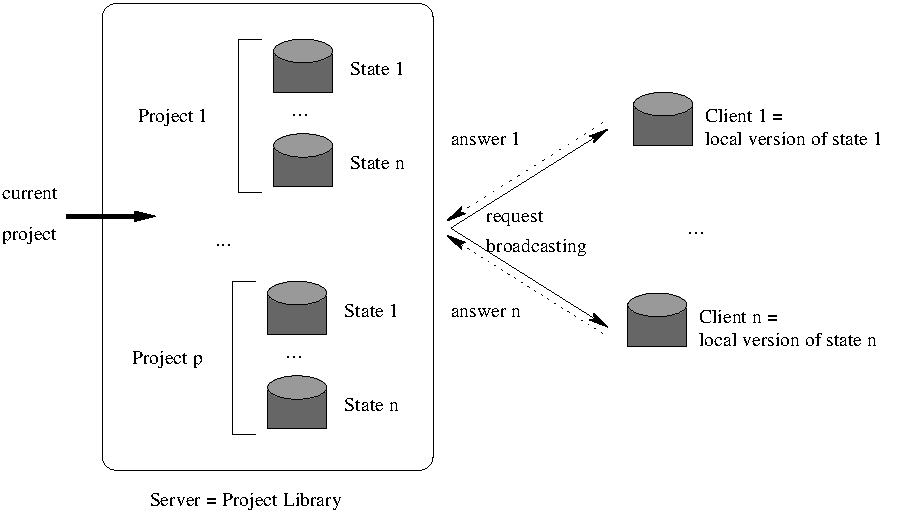
\includegraphics[viewport=0 0 440 246,width=0.99\textwidth]{mecanism.pdf}
    \caption{Interaction between the project library and your registered global
      data.}\label{fig:proj-mechanism}
  \end{figure}

\item It is part of the information saved on disk\index{Saving} for restoration
  in a later session\index{Loading}.
\item It may be part of a \emph{selection}\index{Selection} which is a
  consistent set of states\index{State!Selection|see{Selection}}.
  With such a selection,
  you can control on which states project operations are consistently applied
  (see Section~\ref{proj:selection}). For example, it is possible to clear all
  the states which depend on Value Analysis results.
\item It is possible to ensure inter-analysis consistency\index{Consistency} by
  setting state dependencies\index{State!Dependency}. For example, if the entry
  point\index{Entry Point} of the analyzed program is changed (using
  \texttt{Globals.set\_entry\_point}\scodeidx{Globals}{set\_entry\_point}), all
  the results of analyses depending on it (like value analysis' results) are
  automatically reset. If such a reset were not performed, the results of the
  value analysis would not be consistent anymore with the current entry point,
  leading to incorrect results.
\begin{example}
\sscodeidx{Db}{Value}{is\_computed}
~

\begin{ocamlcode}
Eva.Analysis.compute();
Kernel.feedback "%B" (Eva.Analysis.is_computed ()); (* true *)
Globals.set_entry_point "f" true;
Kernel.feedback "%B" (Eva.Analysis.is_computed ()); (* false *)
\end{ocamlcode}
As the value analysis has been automatically reset when setting the entry point,
the above code outputs
\begin{shell}
[kernel] true
[kernel] false
\end{shell}
\end{example}
\end{itemize}

\subsubsection{State Registration: Overview}
\index{State!Registration|bfit}

For registering a new state, functor
\texttt{State\_builder.Register}\scodeidx{State\_builder}{Register} is
provided. Its use is described in Section~\ref{proj:lowlevel} but it is a
low-level functor which is usually difficult to apply in a correct
way. Higher-level functors are provided to the developer in modules
\texttt{State\_builder}\codeidx{State\_builder} and
\texttt{Cil\_state\_builder}\codeidx{Cil\_state\_builder} that allow the
developer to register states in a simpler way. They internally apply the
low-level functor in the proper way. Module \texttt{State\_builder} provides
state builders for standard \caml datastructures like
hashtables\index{Hashtable} whereas \texttt{Cil\_state\_builder} does the same
for standard \cil datastructures (like hashtables indexed by AST
statements)\footnote{These datastructures are only mutable datastructures (like
  hashtables, arrays and references) because global states are always
  mutable.}. They are described in Section~\ref{proj:computation}.

\begin{important}
  Registering a new state must be performed when the plugin is
  initialized. Thus, using \caml \texttt{let module} construct to
  register the new state is forbidden (except if you really know what
  you are doing).
\end{important}

\subsection{Registering a New State}\label{proj:computation}
\index{State!Registration|bfit}

Here we explain how to register and use a state. Registration through the use of
the low-level functor \texttt{State\_builder.Register} is postponed in
Section~\ref{proj:lowlevel} because it is more tricky and rarely useful.

In most non-\framac applications, a state is a global mutable value. One can use
it to store results of analyses. For example, using this mechanism inside
\framac to create a \texttt{state} which would memoize\index{Memoization} some
information attached to statements would result in the following piece of code.
\scodeidx{Kernel\_function}{t} \scodeidx{Cil\_types}{varinfo}
\sscodeidx{Cil\_datatype}{Stmt}{Hashtbl} \sscodeidx{Db}{Value}{compute}
\begin{ocamlcode}
open Cil_datatype
type info = Kernel_function.t * Cil_types.varinfo
let state : info Stmt.Hashtbl.t = Stmt.Hashtbl.create 97
let compute_info (kf,vi) = ...
let memoize s =
  try Stmt.Hashtbl.find state s
  with Not_found -> Stmt.Hashtbl.add state s (compute_info s)
let run () = ... Eva.Analysis.compute (); ... memoize some_stmt ...
\end{ocamlcode}

However, if one puts this code inside \framac, it does not work because this
state is not registered as a \framac state. For instance, it is never saved on
the disk\index{Saving} and its value is never changed when setting the current
project to a new one. For this purpose, one has to transform the above code into
the following one. \scodeidx{Cil\_state\_builder}{Stmt\_hashtbl}
\scodeidx{Datatype}{Pair} \codeidx{Kernel\_function}
\scodeidx{Cil\_datatype}{Varinfo} \sscodeidx{Db}{Value}{self}
\sscodeidx{Db}{Value}{compute} \codeidx{memo}
\begin{ocamlcode}
module State =
  Cil_state_builder.Stmt_hashtbl
    (Datatype.Pair(Kernel_function)(Cil_datatype.Varinfo))
    (struct
      let size = 97
      let name = "state"
      let dependencies = [ Db.Value.self ]
     end)
let compute_info (kf,vi) = ...
let memoize = State.memo compute_info
let run () = ... Eva.Analysis.compute (); ... memoize some_stmt ...
\end{ocamlcode}
A quick look on this code shows that the declaration of the state itself is more
complicated (it uses a functor application) but its use is
simpler. Actually what has changed?
\begin{enumerate}
\item To declare a new internal state, apply one of the predefined functors in
  modules \texttt{State\_builder}\codeidx{State\_builder} or
  \texttt{Cil\_state\_builder}\codeidx{Cil\_state\_builder} (see interfaces of
  these modules for the list of available modules). Here we use
  \texttt{Cil\_state\_builder.Stmt\_hashtbl} which provides a hashtable indexed
  by statements. The type of values associated to statements is a pair of
  \texttt{Kernel\_function.t} and
  \texttt{Cil\_types.varinfo}\scodeidx{Cil\_types}{varinfo}. The first argument
  of the functor is then the datatype\index{Datatype} corresponding to this type
  (see Section~\ref{type:datatype}). The second argument provides some
  additional information: the initial size of the hashtable\index{Hashtable} (an
  integer similar to the argument of \texttt{Hashtbl.create}), an unique
  name\index{State!Name} for the resulting state and its
  dependencies\index{State!Dependency|bfit}. This list of dependencies is built
  upon values \texttt{self}\codeidxdef{self} which are called \emph{state
    kind}\index{State!Kind|see{Kind}} (or simply \emph{kind}\index{Kind|bfit})
  and are part of any state's module (part of the signature of the low-level
  functor \texttt{State\_builder.Register}%
  \scodeidx{State\_builder}{Register}). This value represents the state itself
  as first-class value (like type values for \caml types, see
  Section~\ref{type:type-value}).
\item From outside, a state actually hides its internal representation in order
  to ensure some invariants: operations on states implementing hashtables do
  not take hashtables as arguments because they implicitly use the hidden
  hashtable. In our example, a predefined memo function is used in order to
  memoize\index{Memoization} the computation of \texttt{compute\_info}. This
  memoization function implicitly operates on the hashtable hidden in the
  internal representation of \texttt{State}.
\end{enumerate}

%\todo{Computation.apply\_once (?)}

\paragraph{Postponed dependencies}\index{State!Dependency!Postponed|bfit}

Sometimes, you want to access a state kind before defining it. That is
usually the case when you have two mutually-dependent states: the dependencies
of the first one provided when registering it must contain the state kind of
the second one which is created by registering it. But this second registration
also requires a list of dependencies containing the first state kind.

For solving this issue, it is possible to postpone the addition of a
state kind to dependencies until all modules have been initialized. However,
dependencies must be correct before anything serious is computed by \framac. So
the right way to do this is the use of the function
\texttt{Cmdline.run\_after\_extended\_stage}% 
\scodeidx{Cmdline}{run\_after\_extended\_stage} (see
Section~\ref{adv:init} for advanced explanation about the way \framac is
initialized).
\begin{example}
Plug-in \texttt{from}\index{From} puts a reference to its state kind in the
following way. This reference is initialized at module initialization time.

\listingname{src/kernel\_services/plugin\_entry\_points/db.mli}
\codeidx{State}
\scodeidx{State}{dummy}
\scodeidx{Db}{From.self}
\begin{ocamlcode}
module From = struct
  ...
  val self: State.t ref
end
\end{ocamlcode}

\listingname{src/kernel\_services/plugin\_entry\_points/db.ml}
\begin{ocamlcode}
module From = struct
  ...
  val self = ref State.dummy (* postponed *)
end
\end{ocamlcode}

\scodeidx{Kernel\_function}{Make\_Table}
\sscodeidx{Db}{Value}{self}
\scodeidx{Db}{From.self}
\listingname{src/plugins/from/functionwise.ml}
\begin{ocamlcode}
module Tbl =
  Kernel_function.Make_Table
    (Function_Froms)
    (struct
       let name = "functionwise_from"
       let size = 97
       let dependencies = [ Db.Value.self ]
     end)
let () =
  (* performed at module initialization runtime. *)
  Db.From.self := Tbl.self
\end{ocamlcode}
Plug-in \texttt{pdg}\index{Plug-in!Pdg|see{Pdg}}\index{Pdg} uses
\texttt{from}\index{From} for computing its own internal state. So it declares
this dependency as follows.

\listingname{src/plugins/pdg/register.ml}
\scodeidx{Kernel\_function}{Make\_Table}
\scodeidx{State\_dependency\_graph}{S.add\_codependencies}
\scodeidx{Cmdline}{run\_after\_extended\_stage}
\begin{ocamlcode}
module Tbl =
  Kernel_function.Make_Table
    (PdgTypes.Pdg)
    (struct
       let name = "Pdg.State"
       let dependencies = [] (* postponed because !Db.From.self may
                                not exist yet *)
       let size = 97
    end)
let () =
  Cmdline.run_after_extended_stage
    (fun () ->
       State_dependency_graph.add_codependencies
         ~onto:Tbl.self
         [ !Db.From.self ])
\end{ocamlcode}
\end{example}

\paragraph{Dependencies over the AST}

Most internal states depend directly or indirectly on the AST of the current
project. However, the AST plays a special role as a state. Namely, it can be
changed in place, bypassing the project mechanism. In particular, it is possible
to add globals. Plugins that perform such changes should inform the kernel
when they are done using
\texttt{Ast.mark\_as\_changed}\scodeidxdef{Ast}{mark\_as\_changed} or 
\texttt{Ast.mark\_as\_grown}\scodeidxdef{Ast}{mark\_as\_grown}. The latter
must be used when the only changes are additions, leaving existing nodes
untouched, while the former must be used for more intrusive changes.
In addition, it is possible to tell the kernel that a state is ``monotonic''
with respect to AST changes, in the sense that it does not need to be cleared
when nodes are added (the information that should be associated to the new 
nodes will be computed as needed). This is done with the function
\texttt{Ast.add\_monotonic\_state}\scodeidxdef{Ast}{add\_monotonic\_state}.
\texttt{Ast.mark\_as\_grown} will not touch such a state, while
\texttt{Ast.mark\_as\_changed} will clear it.

\subsection{Direct Use of Low-level Functor \texttt{State\_builder.Register}}
\label{proj:lowlevel}

Functor \texttt{State\_builder.Register}%
\scodeidxdef{State\_builder}{Register} is the only functor which really
registers a state. All the others internally use it. In some cases (\eg if you
define your own mutable record used as a state), you have to use it. Actually,
in the \framac kernel\index{Kernel}, there are only three direct uses of this
functor over thousands of state registrations: so you will certainly never use
it.

This functor takes three arguments. The first and the third ones respectively
correspond to the datatype\index{Datatype} and to information (name and
dependencies) of the states\index{State!Name}%
\index{State!Dependency}: they are similar to the corresponding
arguments of the high-level functors (see Section~\ref{proj:computation}).

The second argument explains how to handle the \emph{local
  version}\index{State!Local Version|bfit} of the state under
registration. Indeed here is the key point: from the outside, only this local
version is used for efficiency purposes (remember
Figure~\ref{fig:proj-mechanism}). It would work even if projects do not
exist. Each project knows a \emph{global version}\index{State!Global
  Version|bfit}. The project management system \emph{automatically} 
switches\index{Context Switch} the local version when the current
project\index{Project!Current} changes in order to conserve a physical
equality\index{Equality!Physical} between local version and current global
version. So, for this purpose, the second argument provides a type \texttt{t}
(type of values of the state) and five functions \texttt{create} (creation of a
new fresh state), \texttt{clear} (cleaning a state), \texttt{get} (getting a
state), \texttt{set} (setting a state) and \texttt{clear\_some\_projects} (how
to clear each value of type \texttt{project} in the state if any).

\begin{important}
The following invariants must
hold\index{Equality!Physical}\index{Equality!Structural}:\footnotemark
\begin{gather}
\texttt{create ()} \mbox{ returns a fresh value} \label{eq:create}\\
\forall \texttt{p} \mbox{ of type } \texttt{t},\,
\texttt{create () = (clear p; set p; get ())}\label{eq:clear}\\
\forall \texttt{p} \mbox{ of type } \texttt{t},\, \texttt{copy p} \mbox{
  returns a fresh value}
\label{eq:copy}\\
\forall \texttt{p1},\texttt{p2} \mbox{ of type } \texttt{t}
\mbox{ such that } \texttt{p1 != p2},\, \texttt{(set p1; get ()) != p2}
\label{eq:independance}
\end{gather}
\end{important}
\footnotetext{As usual in \caml, \texttt{=} stands for \emph{structural}
  equality while \texttt{==} (resp. \texttt{!=}) stands for \emph{physical}
  equality (resp. disequality).}

Invariant~\ref{eq:create} ensures that there is no sharing%
\index{State!Sharing} with any value of a same state: so each new project has
got its own fresh state. Invariant~\ref{eq:clear} ensures that cleaning
a state\index{State!Cleaning} resets it to its initial
value. Invariant~\ref{eq:copy} ensures that there is no sharing with any
copy. Invariant~\ref{eq:independance} is a local independence criterion which
ensures that modifying a local version does not affect any other version
(different from the global current one) by side effects\index{Side-Effect}.
\begin{example}
  To illustrate this, we show how functor
  \texttt{State\_builder.Ref}\scodeidx{State\_builder}{Ref} (registering a state
  corresponding to a reference) is implemented.
\scodeidx{Datatype}{S}
\begin{ocamlcode}
module Ref
  (Data: Datatype.S)
  (Info: sig include Info val default: unit -> Data.t end) =
struct
  type data = Data.t
  let create () = ref Info.default
  let state = ref (create ())
\end{ocamlcode}
Here we use an additional reference: our local version%
\index{State!Local Version} is a reference on the right value. We can
use it in order to safely and easily implement \texttt{get} and \texttt{set}
required by the registration.
\scodeidx{State\_builder}{Register}
\scodeidx{Datatype}{Ref}
\begin{ocamlcode}
  include Register
    (Datatype.Ref(Data))
    (struct
      type t = data ref (* we register a reference on the given type *)
      let create = create
      let clear tbl = tbl := Info.default
      let get () = !state
      let set x = state := x
      let clear_some_projects f x =
        if Data.mem_project f !x then begin clear x; true end else false
    end)
   (Info)
\end{ocamlcode}
For users of this module, we export ``standard'' operations which hide the
local indirection required by the project management system.
\begin{ocamlcode}
  let set v = !state := v
  let get () = !(!state)
  let clear () = !state := Info.default
end
\end{ocamlcode}
As you can see, the above implementation is error prone; in particular it uses
a double indirection (reference of reference). So be happy that higher-level
functors like \texttt{State\_builder.Ref} are provided which hide such
implementations from you.
\end{example}

\subsection{Using Projects}\label{proj:use}\index{Project!Use|bfit}

As said before, all operations are done by default on the current
project\index{Project!Current}. But sometimes plug-in developers have to
explicitly use another project, for example when the AST is
modified\index{AST!Modification} (usually through the use of a copy
visitor\index{Visitor!Copy}, see Section~\ref{adv:visitors}) or replaced (\eg if
a new one is loaded\index{Loading} from disk).

\begin{important}
  An AST must never be modified inside a
  project\index{AST!Modification}. If such an operation is required, you
  must either create a new project with a new AST, usually by using
  \texttt{File.init\_project\_from\_cil\_file}%
  \scodeidxdef{File}{init\_project\_from\_cil\_file}
  or \texttt{File.init\_project\_from\_visitor}%
  \scodeidxdef{File}{init\_project\_from\_visitor};
  or write the following line of code (see Section~\ref{proj:selection}):
  \scodeidx{Project}{clear}
  \scodeidx{State\_selection}{only\_dependencies}
  \scodeidx{Ast}{self}
  \begin{alltt}
  let selection = State_selection.only_dependencies Ast.self in
  Project.clear ~selection ()
  \end{alltt}
\end{important}

Operations over projects are grouped together in module
\texttt{Project}\codeidxdef{Project}. A project has type
\texttt{Project.t}\scodeidxdef{Project\_skeleton}{t}. Function
\texttt{Project.set\_current}\scodeidxdef{Project}{set\_current} sets the
current project on which all operations are implicitly performed.

\begin{example}\label{ex:set_current}
  Suppose that you saved\index{Saving} the current project into file
  \texttt{foo.sav} in a previous \framac session\index{Session|bfit}\footnote{A
    \emph{session} is one execution of \framac (through \texttt{frama-c} or
    \texttt{frama-c-gui}).} thanks to the following
  instruction.\scodeidx{Project}{save}
\begin{ocamlcode}
Project.save "foo.sav"
\end{ocamlcode}
In a new \framac session, executing the following lines of code (assuming the
value analysis has never been computed previously)
\sscodeidx{Db}{Value}{is\_computed}
\scodeidx{Project}{current}
\scodeidx{Project}{load}
\scodeidx{Project}{set\_current}
\sscodeidx{Db}{Value}{compute}
\scodeidx{Project}{IOError}
\begin{ocamlcode}
let print_computed () =
  Kernel.feedback "%B" (Eva.Analysis.is_computed ())
in
print_computed ();   (* false *)
let old = Project.current () in
try
  let foo = Project.load ~name:"foo" "foo.sav" in
  Project.set_current foo;
  Eva.Analysis.compute ();
  print_computed ();   (* true *)
  Project.set_current old;
  print_computed ()    (* false *)
with Project.IOError _ ->
  Kernel.abort "error while loading"
\end{ocamlcode}
displays
\begin{shell}
[kernel] false
[kernel] true
[kernel] false
\end{shell}
This example shows that the value analysis has been computed only in project
\texttt{foo} and not in project \texttt{old}.
\end{example}

\begin{important}
An important invariant of \framac is: if $p$ is the current project before
running an analysis, then $p$ will be the current project after running it. It
is the responsibility of any plug-in developer to enforce this invariant for
his/her own analysis.
\end{important}

To be sure to enforce the above-mentioned invariant, the project library
provides an alternative to the use of
\texttt{Project.set\_current}\scodeidx{Project}{set\_current}:
\texttt{Project.on}\scodeidxdef{Project}{on} applies an operation on a
given project without changing the current project (\emph{i.e.} locally switch
the current project in order to apply the given operation and, afterwards,
restore the initial context)\index{Context Switch}.
\begin{example}
The following code is equivalent to the one given in
Example~\ref{ex:set_current}.
\begin{ocamlcode}
let print_computed () =
  Value_parameters.feedback "%B" (Eva.Analysis.is_computed ())
in
print_computed ();   (* false *)
try
  let foo = Project.load ~name:"foo" "foo.sav" in
  Project.on foo
    (fun () -> Eva.Analysis.compute (); print_computed () (* true *)) ();
  print_computed ()    (* false *)
with Project.IOError _ ->
  exit 1
\end{ocamlcode}
It displays
\begin{shell}
false
true
false
\end{shell}
\end{example}

\subsection{Selections}\label{proj:selection}\index{Selection|bfit}

Most operations working on a single project (\eg
\texttt{Project.clear}\scodeidx{Project}{clear} or
\texttt{Project.on}\scodeidx{Project}{on}) have an optional parameter
\texttt{selection} of type
\texttt{State\_selection.t}\codeidx{State\_selection}. This parameter allows the
developer to specify on which states\index{State} the operation
applies. A \emph{selection} is a set of states which allows the developer to
consistently handle state dependencies\index{State!Dependency}.
\begin{example}
  The following statement clears all the results of the value analysis and all
  its dependencies in the current project.\index{State!Cleaning}
  \scodeidx{Project}{clear}
  \scodeidx{State\_selection}{with\_dependencies}
  \sscodeidx{Db}{Value}{self}
\begin{ocamlcode}
let selection = State_selection.with_dependencies Db.Value.self in
Project.clear ~selection ()
\end{ocamlcode}
The selection explicitly indicates that we also want to clear all the states
which depend on the value analysis' results\index{State!Dependency}.
\end{example}

\begin{important}
  Use selections carefully: if you apply a function $f$ on a selection $s$ and
  $f$ handles a state which does not belong to $s$, then the computed result by
  \framac is potentially incorrect\index{Consistency}.
\end{important}

\begin{example}
The following statement applies a function \texttt{f} in the project \texttt{p}
(which is not the current one). For efficiency purposes, we restrict the
considered states to the command line options (see Section~\ref{adv:cmdline}).
\scodeidx{Project}{on}
\scodeidxdef{Parameter\_state}{get\_selection}
\begin{ocamlcode}
Project.on ~selection:(Parameter_state.get_selection ()) p f ()
\end{ocamlcode}
This statement only works if \texttt{f} only handles values of the command line
options\index{Command Line!Option}. If it tries to get the value of another
state, the result is unspecified \emph{and all actions using any state of the
  current project\index{Project!Current} and of project \texttt{p} also become
  unspecified}.
\end{example}

%%%%%%%%%%%%%%%%%%%%%%%%%%%%%%%%%%%%%%%%%%%%%%%%%%%%%%%%%%%%%%%%%%%%%%%%%%%%%%%

\section{Command Line Options}\label{adv:cmdline}
\index{Command Line!Option|bfit}

\begin{prereq}
  Knowledge of the \caml module system.
\end{prereq}

Values associated with command line options are called
\emph{parameters}\index{Parameters|bfit}. The parameters of the \framac kernel
are stored in module \texttt{Kernel}\codeidxdef{Kernel} while the
plug-in specific ones have to be defined in the plug-in source
code.

\subsection{Definition}\label{options:definition}

In \framac, a parameter is represented by a value of type
\texttt{Typed\_parameter.t}\scodeidxdef{Typed\_parameter}{t} and by a module
implementing the signature
\texttt{Parameter\_sig.S}\scodeidxdef{Parameter\_sig}{S}. The first
representation is a low-level one required by emitters\index{Emitter} (see
Section~\ref{adv:annotations}) and the GUI. The second one provides a high-level
API: each parameter is indeed a state\index{State} (see
Section~\ref{proj:states}).  Several signatures extending
\texttt{Parameter\_sig.S} are provided in order to deal with the usual parameter
types. For example, there are signatures
\texttt{Parameter\_sig.Int}\scodeidxdef{Parameter\_sig}{Int} and
\texttt{Parameter\_sig.Bool}\scodeidxdef{Parameter\_sig}{Bool} for integer and
boolean parameters. Mostly, these signatures provide getters and setters for
modifying parameter values.

Implementing such an interface is very easy thanks to a set of functors provided
by the output module of
\texttt{Plugin.Register}\scodeidx{Plugin}{Register}. Indeed, you have just to
choose the right functor according to your option type and potentially
the wished default value. Below are some examples of such functors
(see the signature
\texttt{Parameter\_sig.Builder}\scodeidx{Parameter\_sig}{Builder} for an
exhaustive list).
\begin{enumerate}
\item \texttt{False}\sscodeidxdef{Parameter\_sig}{Builder}{False}
  (resp. \texttt{True}\sscodeidxdef{Parameter\_sig}{Builder}{True}) builds a
  boolean option initialized to \texttt{false} (resp. \texttt{true}).
\item \texttt{Int}\sscodeidxdef{Parameter\_sig}{Builder}{Int}
  (resp. \texttt{Zero}\sscodeidxdef{Parameter\_sig}{Builder}{Zero}) builds an
  integer option initialized to a specified value (resp. to \texttt{0}).
\item \texttt{String}\sscodeidxdef{Parameter\_sig}{Builder}{String}
  (resp. \texttt{Empty\_string}
  \sscodeidxdef{Parameter\_sig}{Builder}{Empty\_string}) builds a string option
  initialized to a specified value (resp. to the empty string \texttt{""}).
\item \texttt{String\_set}\sscodeidxdef{Parameter\_sig}{Builder}{String\_set}
  builds an option taking a set of strings in argument (initialized to the empty
  set).
\item
  \texttt{Kernel\_function\_set}%
\sscodeidxdef{Parameter\_sig}{Builder}{Kernel\_function\_set} builds an option
taking a set of kernel functions in argument (initialized to the empty set).
\end{enumerate}
Each functor takes as argument (at least) the name of the command line option
corresponding to the parameter and a short description for this option.

\begin{example}
  The parameter corresponding to the option \texttt{-occurrence} of the plug-in
  \texttt{occurrence} is the module \texttt{Print} (defined in the file
  \texttt{src/plugins/occurrence/options.ml}). It is implemented as follows.
  \sscodeidx{Parameter\_sig}{Builder}{False}
\begin{ocamlcode}
module Print =
  False
    (struct
       let option_name = "-occurrence"
       let help = "print results of occurrence analysis"
     end)
\end{ocamlcode}
So it is a boolean parameter initialized by default to
\texttt{false}. The declared interface for this module is simply
\scodeidx{Parameter\_sig}{Bool}
\begin{ocamlcode}
module Print: Parameter_sig.Bool
\end{ocamlcode}

Another example is the parameter corresponding to the option
\texttt{-impact-pragma} of the plug-in \texttt{impact}. This parameter is
defined by the module \texttt{Pragma} (defined in the file
\texttt{src/plugins/impact/options.ml}). It is implemented as follows.
\sscodeidx{Parameter\_sig}{Builder}{Kernel\_function\_set}
\begin{ocamlcode}
module Pragma =
  Kernel_function_set
    (struct
       let option_name = "-impact-pragma"
       let arg_name = "f1, ..., fn"
       let help = "use the impact pragmas in the code of functions f1,...,fn"
     end)
\end{ocamlcode}
Thus it is a set of \texttt{kernel\_function}s initialized by default to
the empty set. \framac uses
the field \texttt{arg\_name} in order to print the name of the argument when
displaying help. The field \texttt{help} is the help message itself. The
Interface for this module is simple: 
\scodeidx{Parameter\_sig}{Kernel\_function\_set}
\begin{ocamlcode}
module Pragma: Parameter_sig.Kernel_function_set
\end{ocamlcode}
\end{example}

\begin{convention}
Parameters of a same plug-in \texttt{plugin} should belong to a module called
\texttt{Options}, \texttt{Plugin\_options}, \texttt{Parameters} or
\texttt{Plugin\_parameters} inside the plug-in directory.
\end{convention}

Using a kernel parameters or a parameter of your own plug-in is very simple:
you have simply to call the function \texttt{get} corresponding to your
parameter.
\scodeidx{Kernel}{Unicode}
\begin{example}
To know whether \framac uses unicode, just write
\begin{ocamlcode}
Kernel.Unicode.get ()
\end{ocamlcode}

Inside the plug-in \texttt{From}, just write
\scodeidx{From\_parameters}{ForceCallDeps}
\begin{ocamlcode}
From_parameters.ForceCallDeps.get ()
\end{ocamlcode}
in order to know whether callsite-wise dependencies have been required.
\end{example}

Using a parameter of a plug-in $p$ in another plug-in $p'$ requires the use of
module \texttt{Dynamic.Parameter}\scodeidx{Dynamic}{Parameter}: since the
module defining the parameter is not visible from the outside of its plug-in,
you have to use the dynamic API of plug-in $p$ in which $p$'s parameters are
automatically registered (see Section~\ref{adv:dynamic-registration}). The
module \texttt{Dynamic.Parameter} defines sub-modules which provide easy access
to parameters according to their \caml types.
\sscodeidx{Dynamic}{Parameter}{Bool}
\begin{example}
Outside the plug-in \texttt{From}, just write
\begin{ocamlcode}
Dynamic.Parameter.Bool.get "-calldeps" ()
\end{ocamlcode}
in order to know whether callsite-wise dependencies have been required.
\end{example}

\subsection{Tuning}\label{options:tuning}

It is possible to modify the default behavior of command line options in several
ways by applying functions just before or just after applying the functor
defining the corresponding parameter. 

Functions which can be applied afterwards are defined in the output signature of
the applied functor.
\begin{example}
Here is how the option "-slicing-level" restricts the range of its argument to
the interval $[0;3]$.
\begin{ocamlcode}
module Calls =
  Int
    (struct
       let option_name = "-slicing-level"
       let default = 2
       let arg_name = ""
       let help = "..." (* skipped here *)
       end)
let () = Calls.set_range ~min:0 ~max:3
\end{ocamlcode}
\end{example}

Functions which can be applied before applying the functor are defined in the
module \texttt{Parameter\_customize}\codeidxdef{Parameter\_customize}.
\begin{example}
Here is how the opposite of option "-safe-arrays" is renamed into
"-unsafe-arrays" (otherwise, by default, it would be "-no-safe-arrays").
\scodeidx{Parameter\_customize}{set\_negative\_option\_name} 
\scodeidx{Kernel}{SafeArrays}
\begin{ocamlcode}
let () = Parameter_customize.set_negative_option_name "-unsafe-arrays"
module SafeArrays =
  True
    (struct
       let module_name = "SafeArrays"
       let option_name = "-safe-arrays"
       let help = "for arrays that are fields inside structs, assume that €
                   accesses are in bounds"
     end)
\end{ocamlcode}
\end{example}

%%%%%%%%%%%%%%%%%%%%%%%%%%%%%%%%%%%%%%%%%%%%%%%%%%%%%%%%%%%%%%%%%%%%%%%%%%%%%%%

\section{Initialization Steps}\label{adv:init}
\index{Initialization|bfit}
\index{Module Initialization|see{Initialization}}
\index{Plug-in!Initialization|see{Initialization}}

\begin{prereq}
  Knowledge of linking of \caml files.
\end{prereq}

\begin{important}
  In a standard way, \framac modules are initialized in the link
  order\index{Linking} which remains mostly unspecified, so you have to use
  side-effects\index{Side-Effect} at module initialization time carefully.
\end{important}

This section details the different stages of the \framac boot process
to help advanced plug-in developers interact more deeply with
the kernel process. It can also be useful for debugging initialization
problems.

As a general rule, plug-in routines must never be executed at link time. Any
useful code, be it for registration, configuration or \textsf{C}-code analysis,
should be registered as \emph{function hooks} to be executed at a proper time
during the \framac boot process. In general, registering and executing a hook is
tightly coupled with handling the command line parameters.

The parsing of the command line parameters is performed in several
\emph{phases} and \emph{stages}
\index{Command Line!Parsing}, 
each one dedicated to specific operations. For instance,
journal replays should be performed after loading dynamic plug-ins, and so
on. Following the general rule stated at the beginning of this section, even
the kernel services of \framac are internally registered as hooks routines to
be executed at a specific stage of the initialization process, among plug-ins
ones.

From the plug-in developer point of view, the hooks are registered by
calling the \texttt{run\_after\_$xxx$\_stage} routines in
\texttt{Cmdline}\codeidx{Cmdline} module and \texttt{extend} routine
in the \texttt{Db.Main}\sscodeidx{Db}{Main}{extend} module.

The initialization phases and stages of \framac are described below, in
their execution order.

\begin{enumerate}[A --]

\item \textbf{The Initialization Stage:}\index{Initialization} this stage
  initializes \framac compilation units, following some \emph{partially}
  specified order. More precisely:
  \begin{enumerate}[1.]
  \item the architecture dependencies depicted on
    Figure~\ref{fig:architecture} (cf.~p.~\pageref{archi:general}) are
    respected. In particular, the kernel services are linked first,
    \emph{then} the kernel integrated types for plug-ins, and
    \emph{finally} the plug-ins are linked in unspecified order;
  \item when the GUI\index{Plug-in!GUI} is present, for any plug-in
    $p$, the non-gui modules of $p$ are always linked \emph{before}
    the gui modules of $p$;
  \item finally, the module \texttt{Boot}\codeidxdef{Boot} is linked at the
    very end of this stage.
  \end{enumerate}

  Plug-in developers cannot customize this stage. In particular, the module
  \texttt{Cmdline}\codeidx{Cmdline} (one of the first linked modules, see
  Figure~\ref{fig:architecture}) performs a very early configuration stage,
  such as checking if journalization has to be activated
  (cf.~Section~\ref{adv:journalization}\index{Journalization}), or setting the
  global verbosity and debugging levels.

\item \label{stage:early} \textbf{The Early Stage:} this stage initializes the
  kernel services. More precisely:
  \begin{enumerate}[(a)]
  \item first, the journal name is set to its right value (according to the
    option \texttt{-journal-name}) and the default project is created;
  \item then, the parsing of command line options registered for the
    \texttt{Cmdline.Early}\sscodeidxdef{Cmdline}{stage}{Early} stage;
  \item finally, all functions registered through
    \texttt{Cmdline.run\_after\_early\_stage}%
    \scodeidxdef{Cmdline}{run\_after\_early\_stage} are executed in an
    unspecified order.
  \end{enumerate}

\item \label{stage:extending} \textbf{The Extending Stage:}\index{Linking} the searching and
  loading of dynamically linked plug-ins, of journal, scripts and
  modules is performed at this stage. More precisely:

  \begin{enumerate}[(a)]
  \item the command line options registered for the
    \texttt{Cmdline.Extending}\sscodeidxdef{Cmdline}{stage}{Extending} stage
    are treated, such as \texttt{-load-script} and
    \texttt{-add-path};

  \item the hooks registered through
    \texttt{Cmdline.run\_during\_extending\_stage}
    \scodeidxdef{Cmdline}{run\_during\_extending\_stage} are executed. Such
    hooks include kernel function calls for searching, loading and linking the
    various plug-ins, journal and scripts compilation units, with respect to
    the command line options parsed during stages~\ref{stage:early}
    and~\ref{stage:extending}.
  \end{enumerate}

\item \textbf{The Running Phase:} the command line is split into several
  groups of command line arguments, each of them separated by an option
  \texttt{-then} or an option \texttt{-then-on $p$} (thus if there is $n$
  occurrences of \texttt{-then} or \texttt{-then-on $p$}, then there are $n+1$
  groups). For each group, the following stages are executed in sequence: all
  the stages are executed on the first group provided on the command line, then
  they are executed on the second group, and so on.

\begin{enumerate}[1.]

\item \textbf{The Extended Stage:} this step is reserved for commands which
  require that all plug-ins are loaded but which must be executed very
  early. More precisely:

  \begin{enumerate}[(a)]
  \item the command line options registered for the
    \texttt{Cmdline.Extended}\sscodeidxdef{Cmdline}{stage}{Extended} stage
    are treated, such as \texttt{-verbose-*} and \texttt{-debug-*};

  \item the hooks registered through
    \texttt{Cmdline.run\_after\_extended\_stage}%
    \scodeidxdef{Cmdline}{run\_after\_extended\_stage}.
    Most of these registered hooks come from postponed internal-state
    dependencies\index{State!Dependency!Postponed} (see
    Section~\ref{proj:computation}).
  \end{enumerate}

  Remark that both statically and dynamically linked plug-ins have
  been loaded at this stage. Verbosity and debug level for each
  plug-in are determined during this stage.

\item \textbf{The Exiting Stage:} this step is reserved for commands
  that make \framac exit before starting any analysis at all, such as
  printing help information:
  \begin{enumerate}[(a)]

  \item the command line options registered for the
    \texttt{Cmdline.Exiting}\sscodeidxdef{Cmdline}{stage}{Exiting} stage
    are treated;

  \item the hooks registered through
    \texttt{Cmdline.run\_after\_exiting\_stage}
    \scodeidxdef{Cmdline}{run\_after\_exiting\_stage} are executed in
    an unspecified order. All these functions should do nothing (using
    \texttt{Cmdline.nop}\scodeidxdef{Cmdline}{nop}) or raise
    \texttt{Cmdline.Exit}\scodeidxdef{Cmdline}{Exit} for stopping \framac
    quickly.

  \end{enumerate}

\item \textbf{The Loading Stage:} this is where the initial state of \framac
  can be replaced by another one. Typically, it would be loaded from disk
  through the \texttt{-load} option\index{Loading} or computed by running a
  journal (see Section~\ref{adv:journalization})\index{Journalization}. As
  for the other stages:
  \begin{enumerate}[(a)]

  \item first, the command line options registered for the
    \texttt{Cmdline.Loading}\sscodeidxdef{Cmdline}{stage}{Loading} stage
    are treated;

  \item then, the hooks registered through
    \texttt{Cmdline.run\_after\_loading\_stage}
    \scodeidxdef{Cmdline}{run\_after\_loading\_stage} are executed in
    an unspecified order. These functions actually change the initial
    state of \framac with the specified one. The \framac kernel
    verifies as far as possible that only one new-initial state has
    been specified.
  \end{enumerate}

  Normally, plug-ins should never register hooks for this stage unless they
  actually set a different initial state than the default one. In such a case:

  \begin{important}
    They must call the function
    \texttt{Cmdline.is\_going\_to\_load}
    \scodeidxdef{Cmdline}{is\_going\_to\_load} while initializing.
  \end{important}

\item \textbf{The Configuring Stage:} this is the usual place for
  plug-ins to perform special initialization routines if necessary,
  \emph{before} having their main entry points executed. As for
  previous stages:

  \begin{enumerate}[(a)]
  \item first, the command line options registered for the
    \texttt{Cmdline.Configuring}\sscodeidxdef{Cmdline}{stage}{Configuring} stage
    are treated. Command line parameters that do not begin by a hyphen
    (character \texttt{'-'}) are \emph{not} options and are treated as
    \textsf{C} files. Thus they are added to the list of files to be
    preprocessed or parsed for building the \texttt{AST} (on demand);
  \item then, the hooks registered through
    \texttt{Cmdline.run\_after\_configuring\_stage}
    \scodeidxdef{Cmdline}{run\_after\_configuring\_stage} are executed
    in an unspecified order.
  \end{enumerate}

\item \textbf{The Setting Files Stage:} this stage sets the \C files to analyze
  according to those indicated on the command line. More precisely:

  \begin{enumerate}[(a)]
  \item first, each argument of the command line which does not begin by a
    hyphen (character \texttt{'-'}) is registered for later analysis;
  \item then, the hooks registered through
    \texttt{Cmdline.run\_after\_setting\_files}
    \scodeidxdef{Cmdline}{run\_after\_setting\_files} are executed in an
    unspecified order.
  \end{enumerate}

\item \textbf{The Main Stage:} this is the step where plug-ins actually run
  their main entry points registered through
  \texttt{Db.Main.extend}\sscodeidx{Db}{Main}{extend}. For all intents and purposes, you should consider 
  that this stage is the one where these hooks are executed.

\end{enumerate}

\end{enumerate}

%%%%%%%%%%%%%%%%%%%%%%%%%%%%%%%%%%%%%%%%%%%%%%%%%%%%%%%%%%%%%%%%%%%%%%%%%%%%%%%

\section{Customizing the AST creation}\label{sec:customizing-ast}
\begin{prereq}
  None.
\end{prereq}

Plug-ins may modify the way source files are transformed into the AST
over which the analyses are performed. Customization of the front-end of
\framac can be done at several stages.

\begin{enumerate}[A --]
\item\textbf{Parsing:} this stage takes care of converting an individual source
file into a parsed AST (a.k.a Cabs, which differs from the type-checked AST on
which most analyses operate). By default, source files are treated as C files,
possibly needing a pre-processing phase. It is possible to tell Frama-C to use
another parser for files ending with a given suffix by registering this
parser with the \texttt{File.new\_file\_type}\scodeidxdef{File}{new\_file\_type}
function. Suffixes \texttt{.h}, \texttt{.i}, \texttt{.c} and \texttt{.ci}
are reserved for
Frama-C kernel. The registered parser is supposed to return a pair consisting
of a type-checked AST (\verb+Cil_types.file+\scodeidx{Cil\_types}{file}) and
a parsed AST (\verb+Cabs.file+\scodeidx{Cabs}{file}). The former can be obtained
from the latter with the \verb+Cabs2cil.convFile+\scodeidx{Cabs2cil}{convFile}
function, which guarantees that the resulting \verb+Cil_types.file+ respects
all invariants expected by the Frama-C kernel.
\item\textbf{Type-checking:} a normal \verb+Cabs.file+ ({\it i.e.} not obtained
through a custom parsing function) can be transformed before being 
type-checked. Transformation hooks are registered through
\verb+Frontc.add_syntactic_transformation+%
\scodeidxdef{Frontc}{add\_syntactic\_transformation}.
\item\textbf{After linking:} Once all source files have been processed, they
  are all linked together in a single AST. Transformations can be performed
  on the resulting AST at two stages:
  \begin{enumerate}[1.]
  \item before clean-up ({\it i.e.} removal of useless temporary variables
    and prototypes that are never called). At that stage, global tables indexing
    information related to the AST have not yet been filled.
  \item after clean-up. At this stage, index tables are filled, and can thus
    be used. On the other hand, the transformation must take care itself
    of keeping in sync the AST and the tables
  \end{enumerate}
  Registering a transformation for this stage is done through the function
  \verb+File.add_code_transformation_before_cleanup+%
  \scodeidxdefsmall{File}{add\_code\_transformation\_before\_cleanup}
  (respectively \verb+File.add_code_transformation_after_cleanup+%
  \scodeidxdefsmall{File}{add\_code\_transformation\_after\_cleanup}). If such a
  transformation modify the control-flow graph of a function \texttt{f}, in
  particular by adding statements, it must call 
  \verb|File.must_recompute_cfg|\scodeidxdef{File}{must\_recompute\_cfg}, in
  order to have the graph recomputed afterwards.
\end{enumerate}

%%%%%%%%%%%%%%%%%%%%%%%%%%%%%%%%%%%%%%%%%%%%%%%%%%%%%%%%%%%%%%%%%%%%%%%%%%%%%%%

\section{Customizing the machine model}\label{sec:customizing-machdep}
\index{Machine model}

\begin{prereq}
  None.
\end{prereq}

Several aspects of the C standard that are implementation-defined, such as
the width of standard integer types, endianness, signedness of the
\texttt{char} type, etc., as well as a few compiler and architecture specific
features, can be customized using a \texttt{machdep} configuration,
defining a new machine model.

To create a new machine model, define an instance of \verb+Cil_types.mach+%
\scodeidxdef{Cil\_types}{mach}. You can base it on the examples available in
\verb+tests/misc/custom_machdep/custom_machdep.ml+ and
\verb+src/kernel_internals/runtime/machdeps.ml+.
The new definition can be added to \framac's database using
\verb+File.new_machdep+\scodeidxdef{File}{new\_machdep}.

\begin{example}
  A custom machine description may be implemented as follows
  (the meaning of each field is presented later in this section):
\begin{ocamlcode}
let my_machine =
{
  version          = "generic C compiler for my machine";
  compiler         = "generic";
  cpp_arch_flags   = [];
  sizeof_short     = 2;
  sizeof_int       = 4;
  sizeof_long      = 4;
  sizeof_longlong  = 8;
  sizeof_ptr       = 4;
  sizeof_float     = 4;
  sizeof_double    = 8;
  sizeof_longdouble  = 12;
  sizeof_void      = 1;
  sizeof_fun       = 1;
  size_t = "unsigned long";
  wchar_t = "int";
  ptrdiff_t = "int";
  alignof_short = 2;
  alignof_int = 4;
  alignof_long = 4;
  alignof_longlong = 4;
  alignof_ptr = 4;
  alignof_float = 4;
  alignof_double = 4;
  alignof_longdouble = 4;
  alignof_str = 1;
  alignof_fun = 1;
  alignof_aligned = 16;
  char_is_unsigned = false;
  const_string_literals = true;
  little_endian = true;
  underscore_name = false ;
  has__builtin_va_list = true;
}

let () = File.new_machdep "my_machine" my_machine
\end{ocamlcode}
\end{example}

\index{Command Line!-machdep@\texttt{-machdep}}%
After this code is loaded, \framac can be instructed to use the new machine
model using the \texttt{-machdep} command line option.

If you intend to use \framac's standard library headers, you must also do the
following:

\begin{itemize}
\item define constant \verb+__FC_MACHDEP_<CUSTOM>+, replacing \verb+<CUSTOM>+
  with the name (in uppercase letters) of your created machdep;
  this can be done via \verb+-cpp-extra-args="-D__FC_MACHDEP_<CUSTOM>"+;
\item provide a header file with macro definitions corresponding to your \caml
  definitions. For the most part, these are macros prefixed by \verb+__FC_+,
  corresponding to standard C macro definitions, {\it e.g.},
  \verb+__FC_UCHAR_MAX+. These definitions are used by \framac's
  \verb+<limits.h>+ and other headers to provide the standard C definitions.
  The test file \verb+tests/misc/custom_machdep/__fc_machdep_custom.h+
  (reproduced below)
  contains a complete example of the required definitions. Other examples can
  be found in \verb+share/libc/__fc_machdep.h+.
\end{itemize}
Make sure that your custom header defines the \verb+__FC_MACHDEP+
include guard, and that the program you are analyzing includes this header
before all other headers. One way to ensure this without having to modify any
source files is to use an option such as \verb+-include+ in GCC.

\begin{example}
  Contents of \verb+tests/misc/custom_machdep/__fc_machdep_custom.h+, used as
  example for creating custom machdeps. Notice the unusual size for \verb+int+
  (3 bytes), selected for testing purposes only, and inconsistent with the
  chosen values for \verb+INT_MIN+ and \verb+INT_MAX+, which do not fit
  in 3 bytes.
\lstinputlisting{../../tests/misc/custom_machdep/__fc_machdep_custom.h}
\end{example}

An example of the complete command-line is presented below, for a custom
machdep called \texttt{myarch}, defined in file \verb+my_machdep.ml+ and
with stdlib constants defined in \verb+machdep_myarch.h+:

\begin{listing-nonumber}
  frama-c -load-script my_machdep.ml -machdep myarch \
    -cpp-extra-args="-D__FC_MACHDEP_MYARCH -include machdep_myarch.h"
\end{listing-nonumber}

\section{Machdep record fields}\label{sec:machdep-fields}

Each field in the machdep record is succintly described in the \verb+Cil_types+
module. We present below a thorough description of each field.

\begin{description}
\item[\texttt{version}]: human-readable textual description of the machdep.
\item[\texttt{compiler}]: defines whether special compiler-specific extensions
  will be enabled. It should be one of the strings below:
  \begin{itemize}
  \item[\texttt{msvc}]: enables \verb+Cil.msvcMode+, that is,
    MSVC (Visual Studio)-specific extensions;
  \item[\texttt{gcc}]: enables \verb+Cil.gccMode+, that is,
    GCC-specific extensions;
  \item[\texttt{generic}] (or any other string): no special
    compiler-specific extensions.
  \end{itemize}
  Note that some compiler extensions, such as attributes, are always enabled.
\item[\texttt{cpp\_arch\_flags}]: list of arguments to be added to the
  command-line when invoking the C preprocessor. Typically used to ensure that
  multiarch compilers apply the appropriate predefined macros\footnote{Note that
    the sizes of standard integer types are already defined in the machdep,
    so they do not depend on these flags.}.
  E.g. use \verb+["-m32"]+ for a 32-bit machdep when preprocessing with a
  64-bit multiarch GCC.
  Note that, in practice, very few programs rely on such predefined macros,
  such as \verb+__x86_64+ and \verb+__i386+.
  \item[\texttt{sizeof\_short}]: size (in bytes) of the \verb+short+ type.
  \item[\texttt{sizeof\_int}]: size (in bytes) of the \verb+int+ type.
  \item[\texttt{sizeof\_long}]: size (in bytes) of the \verb+long+ type.
  \item[\texttt{sizeof\_longlong}]: size (in bytes) of the \verb+long long+
    type.
    Note that machdeps (for compiler \verb+"gcc"+ in particular) must always
    have at least one type that is 8 bytes wide, which is typically
    \verb+long long+.
  \item[\texttt{sizeof\_ptr}]: size (in bytes) of an object (non-function)
    pointer.
  \item[\texttt{sizeof\_float}]: size (in bytes) of a single-precision floating
    point. In implementations compliant with ISO/IEC/IEEE 60559 -IEEE 754,
    this is always 4.
  \item[\texttt{sizeof\_double}]: size (in bytes) of a double-precision floating
    point. In implementations compliant with ISO/IEC/IEEE 60559 - IEEE 754,
    this is always 8.
  \item[\texttt{sizeof\_longdouble}]: size (in bytes) of a \verb+long double+
    floating point.
    Note: type \verb+long double+ is currently not supported by existing
    \framac plugins,  but this field exists for future expansion, and
    to compute \verb+sizeof+ of aggregates properly.
  \item[\texttt{sizeof\_void}]: the result of evaluating \verb+sizeof(void)+
    by the compiler (or 0 if unsupported).
  \item[\texttt{sizeof\_fun}]: the result of evaluating \verb+sizeof(f)+, where
    \verb+f+ is a function ({\em not} a function pointer) by the compiler
    (or negative if unsupported).
  \item[\texttt{size\_t}]: a string containing the actual type that
    \verb+size_t+ expands to, e.g. \verb+"unsigned long"+.
  \item[\texttt{wchar\_t}]: a string containing the actual type that
    \verb+wchar_t+ expands to. If unsupported, you can use \verb+int+.
  \item[\texttt{ptrdiff\_t}]: a string containing the actual type that
    \verb+ptrdiff_t+ expands to. If unsupported, you can use \verb+int+.
  \item[\texttt{alignof\_short}]: the result of evaluating
    \verb+_Alignof(short)+.
  \item[\texttt{alignof\_int}]: the result of evaluating \verb+_Alignof(int)+.
  \item[\texttt{alignof\_long}]: the result of evaluating \verb+_Alignof(long)+.
  \item[\texttt{alignof\_longlong}]: the result of evaluating
    \verb+_Alignof(long long)+.
  \item[\texttt{alignof\_ptr}]: the result of evaluating \verb+_Alignof(char*)+
    (or any other pointer, including function pointers).
  \item[\texttt{alignof\_float}]: the result of evaluating
    \verb+_Alignof(float)+.
  \item[\texttt{alignof\_double}]: the result of evaluating
    \verb+_Alignof(double)+.
  \item[\texttt{alignof\_longdouble}]: the result of evaluating
    \verb+_Alignof(long double)+.
  \item[\texttt{alignof\_str}]: the result of evaluating \verb+_Alignof("a")+
    (a literal string).
  \item[\texttt{alignof\_fun}]: the result of evaluating \verb+_Alignof(f)+,
    where \verb+f+ is a function (or negative if unsupported).
  \item[\texttt{alignof\_aligned}]: the default alignment of a type having the
    \verb+aligned+ attribute (or 1 if unsupported). This corresponds to the
    default alignment when using \verb+#pragma packed()+ without a numeric
    argument.
  \item[\texttt{char\_is\_unsigned}]: whether type \verb+char+ is unsigned.
  \item[\texttt{const\_string\_literals}]: whether string literals have const
    chars, or are writable. If \verb+true+, the following code has undefined
    behavior, otherwise it is defined: \verb+char *s = "no"; s[0] = 'g';+.
  \item[\texttt{little\_endian}]: whether the machine is little endian.
  \item[\texttt{underscore\_name}]: whether the compiler generates assembly
    labels by prepending \verb+_+ to the identifier. That is, will function
    \verb+foo()+ have the label \verb+foo+, or \verb+_foo+?
  \item[\texttt{has\_\_builtin\_va\_list}]: whether \verb+__builtin_va_list+
    is a (built-in) type known by the preprocessor.
  \item[\texttt{\_\_thread\_is\_keyword}]: whether \verb+__thread+ is a
    keyword (otherwise, it can be used as a standard identifier).
\end{description}

\paragraph{Writing a new machdep}

Writing a machdep for a new architecture is not trivial, due to the fact
that some steps are hard to automate. If you have a working compiler for the
target architecture, you can use it to produce an executable that will print
the contents of expressions such as \verb+sizeof(long)+, \verb+_Alignof(int)+,
etc. You can also use the compiler to test for unsupported features.
In case \verb+printf+ is not available, you can use the exit code of the
program (return code of \verb+main+). In case you can only preprocess, but not
compile and run the program, the assembly code may provide some useful data.

%%%%%%%%%%%%%%%%%%%%%%%%%%%%%%%%%%%%%%%%%%%%%%%%%%%%%%%%%%%%%%%%%%%%%%%%%%%%%%%

\section{Visitors}\label{adv:visitors}\index{Visitor|bfit}

\begin{prereq}
  Knowledge of \caml object programming.
\end{prereq}

Module \texttt{Cil}\codeidx{Cil} offers a visitor\index{Visitor!Cil|bfit},
\verb+Cil.cilVisitor+\scodeidxdef{Cil}{cilVisitor}, 
that allows to traverse (parts of) an
AST\index{AST}. It is a class with one method per type of the AST, whose
default behavior is simply to call the method corresponding to its
children. This is a convenient way to perform local transformations over a
whole \verb+Cil_types.file+\scodeidx{Cil\_types}{file} by inheriting from it
and redefining a few methods. However, the original \cil visitor is of course
not aware of the internal state of \framac itself\index{State}. Hence,
there exists another visitor, \verb+Visitor.generic_frama_c_visitor+%
\scodeidxdef{Visitor}{generic\_frama\_c\_visitor}, which handles
projects\index{Project} in a transparent way for the user. There are very few
cases where the plain \cil visitor should be used.

\begin{important}
  Basically, as soon as the initial project\index{Project!Initial} has been
  built from the C source files (\emph{i.e.} one of the functions
  \texttt{File.init\_$*$}\scodeidx{File}{init\_from\_c\_files}%
  \scodeidx{File}{init\_project\_from\_cil\_file}%
  \scodeidx{File}{init\_project\_from\_visitor}%
  \scodeidx{File}{init\_from\_cmdline} has been applied), only the \framac
  visitor should occur.
\end{important}

There are a few differences between the two (the \framac visitor
inherits from the \cil one).  These differences are summarized in
Section~\ref{adv:sec:diff-betw-cil}, which the reader already familiar with
\cil is invited to read carefully.

\subsection{Entry Points}

Module \texttt{Cil}\codeidx{Cil} offers various entry points for the visitor%
\index{Visitor!Cil!Entry Point}. They are functions called
\verb+Cil.visitCil+\emph{AstType}\scodeidxdef{Cil}{visitCil$AstType$} where
\emph{astType} is a node type in the \cil's AST. Such a function takes as
argument an instance of a \verb+cilVisitor+\scodeidx{Cil}{cilVisitor} and an
\emph{astType} and gives back an \emph{astType} transformed according to the
visitor. The entry points for visiting a whole
\verb+Cil_types.file+\scodeidx{Cil\_types}{file} (\verb+Cil.visitCilFileCopy+%
\scodeidxdef{Cil}{visitCilFileCopy}, \verb+Cil.visitCilFile+%
\scodeidxdef{Cil}{visitCilFile} and \verb+visitCilFileSameGlobals+%
\scodeidxdef{Cil}{visitCilFileSameGlobals}) are slightly different and do not
support all kinds of visitors.  See the documentation attached to them in
\verb+cil.mli+ for more details.

\subsection{Methods}\label{adv:sec:methods}

As said above, there is a method for each type in the \cil AST\index{AST}
(including for logic annotation\index{Annotation}). For a given type
\emph{astType}, the method is called \texttt{v}\emph{astType}\footnote{This
  naming convention is not strictly enforced. For instance the method
  corresponding to \texttt{offset}\scodeidx{Cil\_types}{offset} is
  \texttt{voffs}\sscodeidxdef{Cil}{cilVisitor}{voffs}.}, and has type
\mbox{\emph{astType}$\rightarrow$\emph{astType'}~\texttt{visitAction}}, where
\emph{astType'} is either \emph{astType} or \emph{astType}~\texttt{list} (for
instance, one can transform a \verb+global+\scodeidx{Cil\_types}{global} into
several ones). \texttt{visitAction}\scodeidxdef{Cil}{visitAction} describes
what should be done for the children of the resulting AST node, and is
presented in the next section. In addition, some types have two modes
of visit: one for the declaration and one for use. This is the case for
\verb+varinfo+\scodeidx{Cil\_types}{varinfo}
(\verb+vvdec+\sscodeidxdef{Cil}{cilVisitor}{vvdec} and
\verb+vvrbl+\sscodeidxdef{Cil}{cilVisitor}{vvrbl}),
\verb+logic_var+\scodeidx{Cil\_types}{logic\_var}
(\verb+vlogic_var_decl+\sscodeidxdef{Cil}{cilVisitor}{vlogic\_var\_decl} and
\verb+vlogic_var_use+\sscodeidxdef{Cil}{cilVisitor}{vlogic\_var\_use})
\verb+logic_info+\scodeidx{Cil\_types}{logic\_info}
(\verb+vlogic_info_decl+\sscodeidxdef{Cil}{cilVisitor}{vlogic\_info\_decl} and
\verb+vlogic_info_use+\sscodeidxdef{Cil}{cilVisitor}{vlogic\_info\_use}),
\verb+logic_type_info+\scodeidx{Cil\_types}{logic\_type\_info}
(\verb+vlogic_type_info_decl+\sscodeidxdef{Cil}{cilVisitor}{vlogic\_type\_info\_decl} and
\verb+vlogic_type_info_use+\sscodeidxdef{Cil}{cilVisitor}{vlogic\_type\_info\_use}), and
\verb+logic_ctor_info+\scodeidx{Cil\_types}{logic\_ctor\_info}
(\verb+vlogic_ctor_info_decl+\sscodeidxdef{Cil}{cilVisitor}{vlogic\_ctor\_info\_decl} and
\verb+vlogic_ctor_info_use+\sscodeidxdef{Cil}{cilVisitor}{vlogic\_ctor\_info\_use}).
More detailed information can be found in \verb+cil.mli+.

\begin{important}
  For the \framac visitor, two methods,
  \verb+vstmt+\sscodeidx{Cil}{cilVisitor}{vstmt} 
  and \verb+vglob+\sscodeidx{Cil}{cilVisitor}{vglob} take
  care of maintaining the coherence\index{Consistency} between the transformed
  AST\index{AST!Modification} and the internal state of \framac%
  \index{State}. Thus they must not be redefined. One should redefine
  \verb+vstmt_aux+\sscodeidxdef{Visitor}{frama\_c\_visitor}{vstmt\_aux} and
  \verb+vglob_aux+\sscodeidxdef{Visitor}{frama\_c\_visitor}{vglob\_aux} instead.
\end{important}

\subsection{Action Performed}\label{adv:sec:action-performed}

The return value of visiting methods indicates what should be done
next. There are six possibilities:
\begin{itemize}
\item \verb+SkipChildren+\sscodeidx{Cil}{visitAction}{SkipChildren} the visitor
  does not visit the children;
\item \verb+ChangeTo v+\sscodeidx{Cil}{visitAction}{ChangeTo} the old node is
  replaced by \verb+v+ and the visit stops;
\item \verb+DoChildren+\sscodeidx{Cil}{visitAction}{DoChildren} the visit goes
  on with the children; this is the default behavior;
\item \verb+JustCopy+\sscodeidx{Cil}{visitAction}{JustCopy} is only meaningful
  for the copy visitor. Indicates that the visit should go on with the children,
  but only perform a fresh copy of the nodes
\item \verb+ChangeToPost(v,f)+\sscodeidx{Cil}{visitAction}{ChangeToPost} the old
  node is replaced by \verb+v+, and \verb+f+ is applied to the result. This is
  however not exactly the same thing as returning \verb+ChangeTo(f(v))+. Namely,
  in the case of \verb+vglob_aux+, \verb+f+ will be applied to \verb+v+ only
  \emph{after} the operations needed to maintain the consistency of \framac's
  internal state with respect to the AST have been performed.  Thus,
  \verb+ChangeToPost+ should be used with extreme caution, as \verb+f+ could
  break some invariants of the kernel.
\item \verb+DoChildrenPost f+\sscodeidx{Cil}{visitAction}{DoChildrenPost}
  visit the children and apply the given function to the result.
\item \verb+JustCopyPost(f)+\sscodeidx{Cil}{visitAction}{JustCopyPost}
  is only
  meaningful for the copy visitor. Performs a fresh copy of the nodes
  and all its children and applies \verb+f+ to the copy.
\item
  \verb+ChangeDoChildrenPost(v,f)+%
  \sscodeidx{Cil}{visitAction}{ChangeDoChildrenPost}
  the old node is replaced by \verb+v+, the visit goes on with the children of
  \verb+v+, and when it is finished, \verb+f+ is applied to the result. In the
  case of \verb+vstmt_aux+, \verb+f+ is called after the annotations in the
  annotations table have been visited, but \emph{before} they are attached to
  the new statement, that is, they will be added to the result of
  \verb+f+. Similarly, \verb+vglob_aux+ will consider the
   result of \verb+f+ when filling the table of globals. Note that
   \verb+ChangeDoChildrenPost(x,f)+ where \verb+x+ is the current node
   is \textit{not} equivalent to \verb+DoChildrenPost f+, as in the latter
   case, the visitor mechanism knows that it still deals with the original node.
\end{itemize}

\subsection{Visitors and Projects}\label{sec:visitors-projects}\index{Project}

Copy visitors\index{Visitor!Copy} (see next section) implicitly take an
additional argument, which is the project in which the transformed
AST\index{AST!Modification} should be put in.

Note that the tables of the new project are not filled immediately. Instead,
actions are queued, and performed when a whole
\verb+Cil_types.file+\scodeidx{Cil\_types}{file} has been visited. One can
access the queue with the
\verb+get_filling_actions+\sscodeidxdef{Cil}{cilVisitor}{get\_filling\_actions}
method, and perform the associated actions on the new project with the
\verb+fill_global_tables+\sscodeidxdef{Cil}{cilVisitor}{fill\_global\_tables}
method.

In-place visitors\index{Visitor!In-Place}  always operate on the
current project\index{Project!Current} (otherwise, two projects would
risk sharing\index{Sharing} the same AST\index{AST!Sharing|see{Sharing}}).

\subsection{In-place and Copy Visitors}\label{adv:sec:place-copy-visitors}
\index{Visitor!Behavior|bfit}

The visitors take as argument a
\verb+visitor_behavior+\scodeidx{Cil}{visitor\_behavior}, which comes in two
flavors: \verb+inplace_visit+\scodeidx{Cil}{inplace\_visit}%
\index{Visitor!In-Place|bfit} and \verb+copy_visit+%
\scodeidx{Cil}{copy\_visit}\index{Visitor!Copy|bfit}. In the in-place mode,
nodes are visited in place, while in the copy mode, nodes are copied and the
visit is done on the copy\index{AST!Copying}. For the nodes
shared\index{Sharing} across the AST
(\verb+varinfo+\scodeidx{Cil\_types}{varinfo},
\verb+compinfo+\scodeidx{Cil\_types}{compinfo},
\verb+enuminfo+\scodeidx{Cil\_types}{enuminfo},
\verb+typeinfo+\scodeidx{Cil\_types}{typeinfo},
\verb+stmt+\scodeidx{Cil\_types}{stmt},
\verb+logic_var+\scodeidx{Cil\_types}{logic\_var},
\verb+logic_info+\scodeidx{Cil\_types}{logic\_info} and
\verb+fieldinfo+\scodeidx{Cil\_types}{fieldinfo}), sharing is of course
preserved, and the mapping between the old nodes and their copy can be
manipulated explicitly through the following functions:
\begin{itemize}
\item
  \verb+reset_behavior_+\emph{name}
  \scodeidxdef{Cil}{reset\_behavior\_varinfo}
  resets the mapping corresponding to the type \emph{name}.
\item \verb+get_original_+\emph{name}\scodeidxdef{Cil}{get\_original\_varinfo}
  gets the original value corresponding to a copy (and behaves as the identity
  if the given value is not known).
\item \verb+get_+\emph{name}\scodeidxdef{Cil}{get\_varinfo} gets the copy
  corresponding to an old value. If the given value is not known, it behaves as
  the identity.
\item \verb+set_+\emph{name}\scodeidxdef{Cil}{set\_varinfo} sets a copy for a
  given value. Be sure to use it before any occurrence of the old value has
  been copied, or sharing will be lost.
\end{itemize}

\begin{important}
  \verb+get_original_+\emph{name} functions allow to retrieve additional
  information tied to the original AST nodes. Its result must not be modified
  in place\index{AST!Modification} (this would defeat the purpose of operating
  on a copy to leave the original AST untouched). Moreover, note that whenever
  the index used for \emph{name} is modified in the copy, the internal state of
  the visitor behavior\index{Visitor!Behavior} must be updated accordingly
  (\emph{via} the \verb+set_+\emph{name} function) for
  \verb+get_original_+\emph{name} to give correct results.\index{Consistency}
\end{important}

The list of such indices is given Figure~\ref{fig:idx-visitor}.
\begin{figure}[htbp]
\begin{center}
\begin{tabular}{|l|l|}
  \hline
  Type & Index \\
  \hline
  \verb+varinfo+\scodeidx{Cil\_types}{varinfo} & \verb+vid+ \\
  \hline
  \verb+compinfo+\scodeidx{Cil\_types}{compinfo} & \verb+ckey+ \\
  \hline
  \verb+enuminfo+\scodeidx{Cil\_types}{enuminfo} & \verb+ename+ \\
  \hline
  \verb+typeinfo+\scodeidx{Cil\_types}{typeinfo} & \verb+tname+ \\
  \hline
  \verb+stmt+\scodeidx{Cil\_types}{stmt} & \verb+sid+ \\
  \hline
  \verb+logic_info+\scodeidx{Cil\_types}{logic\_info} &
  \verb+l_var_info.lv_id+ \\
  \hline
  \verb+logic_var+\scodeidx{Cil\_types}{logic\_var} & \verb+lv_id+ \\
  \hline
  \verb+fieldinfo+\scodeidx{Cil\_types}{fieldinfo} & \verb+fname+ and
  \verb+fcomp.ckey+ \\
  \hline
\end{tabular}
\end{center}
\caption{Indices of AST nodes.}\label{fig:idx-visitor}
\end{figure}

\begin{important}
  Last, when using a copy visitor\index{Visitor!Copy}, the actions (see previous
  section) \verb+SkipChildren+\sscodeidx{Cil}{visitAction}{SkipChildren} and
  \verb+ChangeTo+\sscodeidx{Cil}{visitAction}{ChangeTo} must be used with care,
  \emph{i.e.}  one has to ensure that the children are fresh. Otherwise, the new
  AST will share some nodes with the old one.\index{Sharing} Even worse, in such
  a situation the new AST might very well be left in an inconsistent state, with
  uses of shared node ({\it e.g.} a \verb+varinfo+ for a function \verb+f+ in a
  function call) which do not match the corresponding declaration ({\it e.g} the
  \verb+GFun+ definition of \verb+f+).

  When in doubt, a safe solution is to use
  \verb+JustCopy+\sscodeidx{Cil}{visitAction}{JustCopy} instead of
  \verb+SkipChildren+\sscodeidx{Cil}{visitAction}{SkipChildren} and
  \verb+ChangeDoChildrenPost(x,fun x -> x)+%
  \sscodeidx{Cil}{visitAction}{ChangeDoChildrenPost} instead of
  \verb+ChangeTo(x)+\sscodeidx{Cil}{visitAction}{ChangeTo}.
\end{important}

\subsection{Differences Between the \cil and \framac Visitors}
\label{adv:sec:diff-betw-cil}

As said in Section~\ref{adv:sec:methods}, \verb+vstmt+ and \verb+vglob+ should
not be redefined. Use \verb+vstmt_aux+ and \verb+vglob_aux+ instead. Be aware
that the entries corresponding to statements and globals in \framac tables are
considered more or less as children of the node. In particular, if the method
returns \verb+ChangeTo+\sscodeidx{Cil}{visitAction}{ChangeTo} action (see
Section~\ref{adv:sec:action-performed}), it is assumed that it has taken care of
updating the tables accordingly, which can be a little tricky when copying a
\verb+file+\scodeidx{Cil\_types}{file}\index{AST!Copying} from a project to
another one. Prefer
\verb+ChangeDoChildrenPost+\sscodeidx{Cil}{visitAction}{ChangeDoChildrenPost}.
On the other hand, a
\verb+SkipChildren+\sscodeidx{Cil}{visitAction}{SkipChildren} action implies
that the visit will stop, but the information associated to the old value will
be associated to the new one. If the children are to be visited, it is undefined
whether the table entries are visited before or after the children in the AST.

\subsection{Example}

Here is a small copy visitor that adds an assertion for each
division in the program, stating that the divisor is not zero:
\scodeidx{Visitor}{generic\_frama\_c\_visitor}
\scodeidx{Cil}{copy\_visit}
\scodeidx{Cil}{lzero}
\sscodeidx{Cil}{cilVisitor}{vexpr}
\sscodeidx{Cil\_types}{exp\_node}{BinOp}
\sscodeidx{Cil\_types}{relation}{Rneq}
\sscodeidx{Cil\_types}{binop}{Div}
\sscodeidx{Cil\_types}{binop}{Mod}
\scodeidx{Logic\_utils}{expr\_to\_term}
\scodeidx{Logic\_const}{prel}
\sscodeidx{Cil}{cilVisitor}{get\_filling\_actions}
\sscodeidx{Cil}{visitAction}{DoChildren}
\scodeidx{File}{create\_project\_from\_visitor}
\scodeidx{Annotations}{add\_assert}
\sscodeidx{Db}{Main}{extend}
\scodeidx{Cil}{get\_stmt}
\scodeidx{Cil}{get\_kernel\_function}
\sscodeidx{Cil}{cilVisitor}{behavior}
\scodeidx{Ast}{self}
\sscodeidx{Cil}{cilVisitor}{current\_kinstr}
\sscodeidx{Visitor}{frama\_c\_visitor}{current\_kf}
\ocamlinput{./examples/generated/syntactic_check.ml}

%%%%%%%%%%%%%%%%%%%%%%%%%%%%%%%%%%%%%%%%%%%%%%%%%%%%%%%%%%%%%%%%%%%%%%%%%%%%%%%

\section{Logical Annotations}\label{adv:annotations}\index{Annotation|bfit}

\begin{prereq}
  None.
\end{prereq}

Logical annotations set by the users in the analyzed \C program are part of the
AST\index{AST}. However others annotations (those generated by plug-ins) are
not directly in the AST because it would contradict the rule ``an AST must
never be modified inside a project'' (see Section~\ref{proj:use}).

So all the logical annotations (including those set by the users) are put in
global projectified tables maintained up-to-date by the \framac kernel. Anytime
a plug-in wants either to access to or to add/delete an annotation, it
\emph{must} use the corresponding modules or functions and not the annotations
directly stored in the AST. These modules and functions are the following.
\begin{itemize}
\item Module \texttt{Annotations}\codeidxdef{Annotations} which contains the
  database of annotations related to the AST (global annotations, function
  contracts and code annotations). Adding or deleting an annotation requires to
  define an emitter by \texttt{Emitter.create}\scodeidx{Emitter}{create} first.
\item Module \texttt{Property\_status}\codeidxdef{Property\_status} should
  be used to get or to modify the validity status of logical
  properties. Modifying a property status requires to define an emitter by
  \texttt{Emitter.create}\scodeidx{Emitter}{create} first. Key concepts and
  theoretical foundation of this module are described in an associated research
  paper~\cite{fmics12}.
\item Module \texttt{Property}\codeidxdef{Property} provides access to all
  logical properties on which property statuses can be emitted. In particular,
  an ACSL annotation has to be converted into a property if you want to access
  its property statuses.
\item Modules \texttt{Logic\_const}\codeidxdef{Logic\_const},
  \texttt{Logic\_utils}\codeidxdef{Logic\_utils} and
  \texttt{Db.Properties}\scodeidxdef{Db}{Properties} contain several
  operations over annotations.
\end{itemize}

%%%%%%%%%%%%%%%%%%%%%%%%%%%%%%%%%%%%%%%%%%%%%%%%%%%%%%%%%%%%%%%%%%%%%%%%%%%%%%%

\section{Extending ACSL annotations}\label{sec:extend-acsl-annot}
\begin{prereq}
  Knowledge of the ACSL specification language.
\end{prereq}

\framac supports the possibility of adding specific ACSL annotations in the
form of special clauses.
Such clauses can be of different categories, as described by
\scodeidx{Cil\_types}{ext\_category}\texttt{Cil\_types.ext\_category}.
\begin{itemize}
\item A contract extension will be
stored in the \texttt{b\_extended}\sscodeidx{Cil\_types}{behavior}{b\_extended} field of
\texttt{Cil\_types.behavior}\scodeidx{Cil\_types}{behavior}.
\item A global extension will be found as a global ACSL annotation in the form of a
\scodeidx{Cil\_types}{Dextended}\texttt{Cil\_types.Dextended} constructor.
\item A code annotation extension will be stored with an
\scodeidx{Cil\_types}{AExtended}\texttt{Cil\_types.AExtended} constructor. Such an extension has itself
different flavors, determined by the \scodeidx{Cil\_types}{ext\_code\_annot\_context} type:
\begin{itemize}
\item it can be meant to be evaluated exactly at the current program point
 (like an ACSL \texttt{assert}), or
\item it can be related to the next statement (or block), like an ACSL statement contract, or
\item it can be a loop extension, or
\item it can be used both as a loop extension or be related to the next (non-loop) statement.
\end{itemize}
\end{itemize}

An extension is characterized by its introducing keyword \texttt{kw}, or \texttt{loop kw} for a loop
extension. It is not possible to have the same keyword for two distinct extensions, especially if
they belong to different categories, as this would lead to ambiguities in the parser.

Once an extension is registered a clause of the form \verb|kw e1,...,en;|, where each \verb|ei| can be
any syntactically valid ACSL term or predicate, will be treated by the parser as belonging to the
extension \verb|kw|.

Contract extension clauses must occur after \verb|assumes| and \verb|requires| clauses if any, but
can be freely mixed with other behavior clauses (post-conditions, \verb|assigns|, \verb|frees| and
\verb|allocates|).

Similarly, in a loop annotation, \verb|loop kw e1, ..., en;| will be treated as belonging to the
\verb|kw| extension. In case the loop annotation has a \verb|loop variant|, the extension must 
occur before. Otherwise, there is no ordering constraint with other loop annotations clauses.

Global extensions can appear either alone in a global annotation, or as part of an axiomatic with
a set of other global annotations.

Finally, a code annotation extension must appear as a single code annotation, like any code annotation.

Code (and loop) extensions can be made specific to a
set of existing behaviors using the standard ACSL \verb|for| construction.
Namely, \verb|for bhv: loop kw e1, ..., en;| will indicate that the
(loop) extension is supposed to be considered only when behavior \verb|bhv| is
active (although it is ultimately up to the plugin to decide what to do with
this information).

An \texttt{acsl\_extension}\scodeidx{Cil\_types}{acsl\_extension} is a triple
\texttt{(id, kw, ext)} where \texttt{id} is its unique ID, used in annotation tables and generated
by \scodeidx{Logic\_const}{new\_acsl\_extension}\texttt{Logic\_const.new\_acsl\_extension},
\texttt{kw} identifies the extension, and \texttt{ext} is an
\texttt{acsl\_extension\_kind}\scodeidx{Cil\_types}{acsl\_extension\_kind}
and can take three forms:
\begin{itemize}
\item \texttt{Ext\_id id} with \texttt{id} an \texttt{int}
that the plugin can use to refer to the annotation in its internal state.
This identifier is under the full responsibility of the plugin
 and will never be used by the kernel.
\item \texttt{Ext\_preds preds} with \texttt{preds} a possibly empty list of
predicates.
\item \texttt{Ext\_terms terms} with \texttt{terms} a possibly empty list of
  terms.
\end{itemize}
For the latter two cases,
the corresponding list is traversed normally by the visitor
(see section~\ref{adv:visitors}).

In order for the extension to be recognized by the parser, it must be
registered by one of the following functions, depending on its category.
\begin{itemize}
\item \texttt{Acsl\_extension.register\_behavior}%
\scodeidx{Acsl\_extension}{register\_behavior}
\item \texttt{Acsl\_extension.register\_global}%
\scodeidx{Acsl\_extension}{register\_global}
\item \texttt{Acsl\_extension.register\_code\_annot}%
\scodeidx{Acsl\_extension}{register\_code\_annot}
\item \texttt{Acsl\_extension.register\_code\_annot\_next\_stmt}%
\scodeidx{Acsl\_extension}{register\_code\_annot\_next\_stmt}
\item \texttt{Acsl\_extension.register\_code\_annot\_next\_loop}%
\scodeidx{Acsl\_extension}{register\_code\_annot\_next\_both}
\item \texttt{Acsl\_extension.register\_code\_annot\_next\_both}%
\scodeidx{Acsl\_extension}{register\_code\_annot\_next\_loop}
\end{itemize}

Each function takes the following mandatory arguments:
\begin{itemize}
\item \texttt{kw} the name of the extension,
\item \texttt{typer} the type-checking function itself.
\item \texttt{status}, a boolean flag indicating whether the extended
  annotation may have a validity status, and

\end{itemize}

During type-checking, the list \verb|[e1;...;en]| will be given to \verb|typer|,
together with the current typing environment (which allows discriminating
between contract and loop extensions and will have the appropriate logic labels
set in the local environment). \verb|typer| must return the corresponding
\verb|acsl_extension_kind| (possibly adding an entry for key \verb|id|
in an internal table if it chooses to return \verb|Ext_id id|).

The first argument of \verb|typer| is a \verb|Logic_typing.typing_context|%
\scodeidx{Logic\_typing}{typing\_context} which provides lookup functions for the
various kinds of identifiers that are present in the environment, as well as
extensible type-checking functions for predicates, terms, and assigns clauses.
Indeed, these functions take themselves as argument a \verb|typing_context|
\verb|ctxt| and will use the functions of \verb|ctxt| to type-check the children
of the current node. Extensions can take advantage of this open recursion to
recognize only subtrees of an otherwise normal ACSL predicate or term. For
instance, the following code will let extension \verb|foo| replace all
occurrences of \verb|\foo| by \verb|42|.

\ocamlinput{./examples/acsl_extension_foo.ml}

With this extension enabled, \framac will interpret the following clause in
a given source file:
\begin{lstlisting}[language=C,alsolanguage=ACSL]
/*@ foo 84 == \foo + \foo; */
\end{lstlisting}
as the following type-checked AST fragment:
\begin{lstlisting}[language=C,alsolanguage=ACSL]
/*@ foo 84 == 42 + 42; */
\end{lstlisting}

If the extended clause is of kind \verb|Ext_preds l| or \verb|Ext_terms l|,
and all the information of the extension is contained in the list \verb|l|,
no function other than the typing function needs to be registered. The parsing
will use the standard way to parse untyped predicates and terms. After
typing, the visitor will traverse each element of \verb|l| as well as any
predicate or term present in the AST. The pretty-printer will output these
elements as a comma-separated list preceded by \verb|kw| (or \verb|loop kw| if
the extension is a loop annotation).

However, depending on the situation, the following optional functions can be
provided to the registration function in order to modify how ACSL extensions
are handled by Frama-C:

\begin{itemize}
\item \texttt{preprocessor} a transformer to apply on the untyped term or
  predicate read during the parsing phase,
\item \texttt{visitor} the visitor function to be applied when visiting
  the extension,
\item \texttt{printer} the pretty-printing function associated to the
  extension,
\item \texttt{short\_printer} a function used to provide a brief textual
  representation of an extension.
\end{itemize}

The \verb|preprocessor| function is applied just after parsing the extension
terms. It takes the list of untyped terms or predicates and can either return
the same list (but reading it to do some stuff) or return a new list. By
default, this function is the identity.

The \verb|visitor| function is used by the Frama-C visitors. It takes the
current visitor, together with the \verb|acsl_extension_kind| of the extended
clause and must returns a \verb|Cil.visitAction|. By default, this function
just returns \verb|Cil.DoChildren|.

The \verb|printer| function is used by the \verb|Cil_printer.pp_extended|
function. It takes the current pretty-printer, the formatter, together with
the \verb|acsl_extension_kind| of the extended clause. By default, it prints
the list of terms or predicates if the kind is \verb|Ext_preds l| or
\verb|Ext_terms l|. If the kind is \verb|Ext_id i|, it only prints the
integer \verb|i|.

The \verb|short_printer| function is a function that can be useful for
debugging or user-feedback. As an alternative to \verb|Cil_printer.pp_extended|,
the \verb|Cil_printer.pp_short_extended| can be used to get brief description
of the content of the extension. It is for example used by the GUI to get
a more informative name for the extension in the file tree. By default, it
does not print anything about the content of the extension, so that the
result is \verb|"kwd"| or \verb|"loop kwd"|.

When the extension kind is \verb|Ext_id|, it is common that the plugin
defining the extension contains a table that associates some data to this
identifier. In such a case, a \verb|printer| might be needed to reconstruct
the source code from the data so that a pretty printed code can be parsed
again. For the same reason, an extension that registers a \verb|preprocessor|
that modifies the AST should probably register a \verb|printer| to recover
the original content.

It is also common, when the kind is \verb|Ext_id|, to define a particular
visitor for the extension, either to ignore the content of the extension as
it is in an internal table of the plugin (thus returning a \verb|SkipChildren|
action) or, on the opposite, to give the possibility to a user defined visitor
to get an access to this content.

The following code shows a more complete extension example. It provides the
user a way to load some types (assumed to be external to Frama-C) so that they
can be used in ACSL specification.

\ocamlinput{./examples/acsl_extension_ext_types.ml}

Namely, specification:

\begin{lstlisting}[language=C,alsolanguage=ACSL]
/*@ ext_type load: foo ; */
/*@ 
  axiomatic Pred {
    predicate P(foo f) reads \nothing ;
  }
*/
/*@ lemma X: \forall foo f ; P(f) ; */
\end{lstlisting}

is correctly parsed and typed by Frama-C and leads to the following displayed
version in the interface:

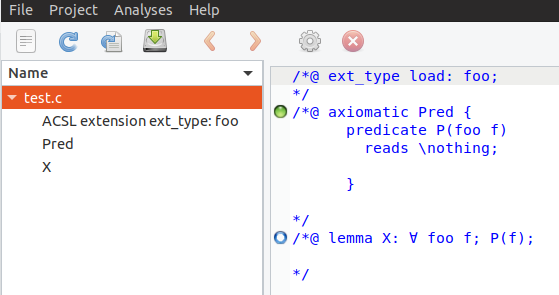
\includegraphics[width=\textwidth]{examples/acsl_extension_ext_types}



%%%%%%%%%%%%%%%%%%%%%%%%%%%%%%%%%%%%%%%%%%%%%%%%%%%%%%%%%%%%%%%%%%%%%%%%%%%%%%%

\section{Locations}\label{adv:memory}\index{Location|bfit}

\begin{prereq}
  None.
\end{prereq}

In \framac, different representations of \C locations
exist. Section~\ref{memory:repr} presents them. Moreover, maps indexed by
locations are also provided. Section~\ref{memory:map} introduces them.

\subsection{Representations}\label{memory:repr}

There are four different representations of \C locations. Actually only three
are really relevant. All of them are defined in module
\texttt{Locations}\codeidxdef{Locations}. They are introduced below. See the
documentation of \texttt{src/kernel\_services/abstract\_interp/locations.mli}
for details about the provided operations on these types.

\begin{itemize}
\item Type \texttt{Location\_Bytes.t}\scodeidxdef{Locations}{Location\_Bytes}
  is used to represent values of \C expressions like \texttt{2} or
  \texttt{((int) \&a) + 13}. With this representation, there is no way to know
  the size of a value while it is still possible to join two values. Roughly
  speaking it is represented by a mapping between \C variables and offsets in
  bytes.
\item Type \texttt{location}\scodeidxdef{Locations}{location}, equivalently
  \texttt{Location.t}\scodeidxdef{Locations}{Location} is used to represent the
  right part of a \C affectation (including bitfields). It is represented by a
  \texttt{Location\_Bits.t} (see below) attached to a size. It is possible to
  join two locations \emph{if and only if they have the same sizes.}
\item Type \texttt{Location\_Bits.t}\scodeidxdef{Locations}{Location\_Bits} is
  similar to \texttt{Location\_Bytes.t} with offsets in bits instead of
  bytes. Actually it should only be used inside a location.
\item Type \texttt{Zone.t}\scodeidx{Locations}{Zone} is a set of bits (without
  any specific order). It is possible to join two zones \emph{even if they have
    different sizes}.
\end{itemize}

\begin{convention}
  Roughly speaking, locations and zones have the same purpose. You should use
  locations as soon as you have no need to join locations of different sizes.
  If you require to convert locations to zones, use the function
  \texttt{Locations.enumerate\_valid\_bits}%
  \scodeidxdef{Locations}{enumerate\_valid\_bits}.
\end{convention}

As join operators are provided for these types, they can be easily used in
abstract interpretation analyses\index{Abstract Interpretation} (which can
themselves be implemented thanks to one of functors of module
\texttt{Dataflow2}\codeidx{Dataflow}.

\subsection{Map Indexed by Locations}\label{memory:map}

Modules \texttt{Lmap}\codeidxdef{Lmap} and
\texttt{Lmap\_bitwise}\codeidxdef{Lmap\_bitwise} provide functors implementing
maps indexed by locations and zones (respectively). The argument of these
functors have to implement values attached to indices (resp. locations or zones).

These implementations are quite more complex than simple maps because they
automatically handle overlaps of locations (or zones). So such implementations
actually require that the structures implementing the values attached to indices
are at least semi-lattices\index{Lattice}; see the corresponding signatures
in module \texttt{Lattice\_type}\codeidx{Lattice\_type}. For
this purpose, functors of the abstract interpretation toolbox%
\index{Abstract Interpretation} can help (see in particular module
\texttt{Abstract\_interp}\codeidx{Abstract\_interp}).

%%%%%%%%%%%%%%%%%%%%%%%%%%%%%%%%%%%%%%%%%%%%%%%%%%%%%%%%%%%%%%%%%%%%%%%%%%%%%%%

\section{GUI Extension}\label{adv:gui}\index{GUI|bfit}\index{Plug-in!GUI|bfit}

\begin{prereq}
  Knowledge of \lablgtk.
\end{prereq}

Each plug-in can extend the \framac graphical user interface (aka \emph{GUI})
in order to support its own functionalities in the \framac viewer. For this
purpose, a plug-in developer has to register a function of type
\texttt{Design.main\_window\_extension\_points \fl~unit} thanks to
\texttt{Design.register\_extension}\scodeidx{Design}{register\_extension}. The
input value of type \texttt{Design.main\_window\_extension\_points} is an
object corresponding to the main window of the \framac GUI. It provides
accesses to the main widgets of the \framac GUI and to several plug-in extension
points. The documentation of the class type
\texttt{Design.main\_window\_extension\_points}%
\scodeidxdef{Design}{main\_window\_extension\_points} is accessible through the
source documentation (see Section~\ref{adv:documentation}).

The GUI plug-in code has to be put in separate files into the plug-in
directory\index{Plug-in!Directory}. Furthermore, in the
\texttt{Makefile}\codeidx{Makefile}, the variable
\texttt{PLUGIN\_GUI\_CMO}\codeidx{PLUGIN\_GUI\_CMO} has to be set in order to
compile the GUI plug-in code (see Section~\ref{make:plugin}).

Besides time-consuming computations have to call the function
\texttt{!Db.progress}\scodeidx{Db}{progress} from time to time in order to keep the GUI reactive.

%Mainly that's all! 
The GUI implementation uses
\lablgtk~\cite{lablgtk}\index{Lablgtk}: you can use any \lablgtk-compatible
code in your gui extension. A complete example of a GUI extension may be found in
the plug-in \texttt{Occurrence}\index{Occurrence} (see file
\texttt{src/plugins/occurrence/register\_gui.ml}).

\begin{important}
\paragraph{Potential issues}
All the GUI plug-in extensions share the same window and same
widgets\index{Sharing!Widget}. So conflicts can occur, especially if you
specify some attributes on a predefined object. For example, if a plug-in wants
to highlight\index{Highlighting} a statement $s$ in yellow and another one
wants to highlight $s$ in red at the same time, the behavior is not specified
but it could be quite difficult to understand for an user.
\end{important}

%%%%%%%%%%%%%%%%%%%%%%%%%%%%%%%%%%%%%%%%%%%%%%%%%%%%%%%%%%%%%%%%%%%%%%%%%%%%%%%

\section{Documentation}\label{adv:documentation}
\index{Documentation|bfit}

\begin{prereq}
  Knowledge of \ocamldoc.
\end{prereq}

Here we present some hints on the way to document your plug-in. First
Section~\ref{doc:rules} introduces a quick general overview about the
documentation process. Next Section~\ref{doc:plugin} focuses on the
plug-in source documentation.

\subsection{General Overview}\label{doc:rules}

Command \texttt{make doc}\codeidx{Makefile} produces the whole \framac source
documentation\index{Documentation!Source} in HTML format. The generated index
file is \texttt{doc/code/html/index.html}. A more general purpose index is
\texttt{doc/index.html}\codeidx{index.html} (from which the previous index is
accessible).

The previous command takes times. So command \texttt{make doc-kernel} only
generates the kernel documentation\index{Documentation!Kernel} (\emph{i.e.}
\framac without any plug-in) while \texttt{make \$(PLUGIN\_NAME)\_DOC} (by
substituting the right value for
\texttt{\$(PLUGIN\_NAME)})\codeidx{PLUGIN\_NAME} generates
the documentation for a single plug-in\index{Plug-in!Documentation}%
\index{Documentation!Plug-in|see{Plug-in Documentation}}.

\subsection{Source Documentation}\label{doc:plugin}
\index{Plug-in!Documentation|bfit}

Each plug-in should be properly documented. \framac uses \ocamldoc and so you
can write any valid \ocamldoc comments.

\paragraph{\ocamldoc tags for \framac}\index{Documentation!Tags} The tag
\texttt{@since version} should document any element introduced after the very
first release, in order to easily know the required version of the \framac
kernel or specific plug-ins. In the same way, the \framac documentation
generator provides a custom tag \texttt{@modify version description} which
should be used to document any element which semantics have changed since its
introduction.

Furthermore, the special tag \texttt{@plugin developer guide} must be attached
to each function used in this document.

\paragraph{Plug-in API}

A plug-in should export functions in its plug-in interface or through modules
\texttt{Db}\codeidx{Db} or \texttt{Dynamic}\codeidx{Dynamic} as explained in
Section~\ref{adv:plugin-registration}.

\begin{important}
The interface name of a plug-in \texttt{plugin} must be \texttt{Plugin.mli}. Be
careful to capitalization of the filename which is unusual in \caml but
required here for compilation purposes.
\end{important}

\paragraph{Internal Documentation for Kernel Integrated Plug-ins}

The \framac documentation generator also produces an internal plug-in
documentation which may be useful for the plug-in developer itself. This
internal documentation is available \emph{via} file
\texttt{doc/code/$plugin$/index.html}\codeidx{index.html} for each plug-in
$plugin$. You can add an introduction to this documentation into a file. This
file has to be assigned into variable
\texttt{PLUGIN\_INTRO}\codeidx{PLUGIN\_INTRO} of the
\texttt{Makefile}\codeidx{Makefile} (see Section~\ref{make:plugin}).

In order to ease access to this internal documentation, you have to
manually edit the file \texttt{doc/index.html}\codeidx{index.html} in order to add
an entry for your plug-in in the plug-in list.

\paragraph{Internal Documentation for External Plug-ins}

External plug-ins can be documented in the same way as plug-ins that are 
compiled together with \framac. However, in order to be able to compile the
documentation with \texttt{make doc}, you must have generated the documentation
of Frama-C's kernel (\texttt{make doc}, see above) and installed it with the 
\texttt{make install-doc-code}\codeidx{install-doc-code} command.

%%%%%%%%%%%%%%%%%%%%%%%%%%%%%%%%%%%%%%%%%%%%%%%%%%%%%%%%%%%%%%%%%%%%%%%%%%%%%%%

%% \section{License Policy}\label{adv:copyright}\index{License|bfit}

%% \begin{target}developers with a SVN access.\end{target}

%% \begin{prereq}
%% knowledge of \make.
%% \end{prereq}

%% If you want to redistribute a plug-in inside \framac, you have to define a
%% proper license policy\index{Plug-in!License}. For this purpose, some help is
%% provided in the \texttt{Makefile}\codeidx{Makefile}. Mainly we distinguish two
%% cases described below.
%% \begin{itemize}
%% \item \textbf{If the wished license is already used inside \framac}, just
%%   extend the variable corresponding to the wished license in order to include
%%   files of your plug-in. Next run \texttt{make headers}\index{Header}.
%%   \begin{example}
%%     Plug-in \texttt{slicing}\index{Slicing}\index{Plug-in!Slicing|see{Slicing}}
%%     is released under LGPL\index{LGPL} and is proprietary of both CEA and
%%     INRIA\index{Copyright}. Thus, in the \texttt{Makefile}, there is the following line.
%%     \codeidx{CEA\_INRIA\_LGPL}
%%     \begin{makefilecode}
%% CEA_INRIA_LGPL= ... €
%%                  src/plugins/slicing/*.ml*
%%      \end{makefilecode}
%%   \end{example}
%% \item \textbf{If the wished license is unknown inside \framac}, you have to:
%%   \begin{enumerate}
%%   \item Add a new variable $v$ corresponding to it and assign files of your
%%     plug-in;
%%   \item Extend variable \texttt{LICENSES}\codeidx{LICENSES} with
%%     this variable;
%%   \item Add a text file in directory \texttt{licenses}\codeidx{licenses}
%%     containing your licenses
%%   \item Add a text file in directory \texttt{headers}\codeidx{headers}
%%     containing the headers\index{Header} to add into files of your plug-in
%%     (those assigned by $v$).

%%     \begin{important}
%%       The filename must be the same than the variable name $v$. Moreover this
%%       file should contain a reference to the file containing the whole license
%%       text.
%%     \end{important}
%%   \item Run \texttt{make headers}.
%%   \end{enumerate}
%% \end{itemize}

% Local Variables:
% ispell-local-dictionary: "english"
% TeX-master: "main"
% End:

%; whizzy-master "developpeur.tex"

\chapter{Reference Manual}\label{chap:refman}

\begin{target}
Developers who would like to have a deep understanding of \framac.
\end{target}

This chapter is a reference manual for \framac developers. It provides details
completing the previous chapters.

%%%%%%%%%%%%%%%%%%%%%%%%%%%%%%%%%%%%%%%%%%%%%%%%%%%%%%%%%%%%%%%%%%%%%%%%%%%%%%%

\section{Configure.in} \label{refman:configure}\codeidxdef{configure.in}

Figure~\ref{fig:configure-sections} presents the different parts of
\texttt{configure.in} in the order in which they are introduced in the file. The
second column of the table indicates whether the given part might need
to be modified by a kernel-integrated plug-in
developer\index{Plug-in!Kernel-integrated}. More details are provided below.
\begin{figure}[htbp]
\begin{center}
\begin{tabular}{|c|c|c|c|}
\hline
\textbf{Id} & \textbf{Name} & \textbf{Mod.} & \textbf{Reference} \\
\hline \hline
1 & Configuration of \make & no & \\
2 & Configuration of \caml & no & \\
3 & Configuration of mandatory tools/libraries & no & \\
4 & Configuration of non-mandatory tools/libraries & no & \\
5 & Platform configuration & no & \\
6 & Wished \framac plug-in & \textbf{yes} &  Sections~\ref{conf:add}
and~\ref{conf:dep-lib}\\
7 & Configuration of plug-in tools/libraries & \textbf{yes} & Section~\ref{conf:lib} \\
8 & Checking plug-in dependencies & \textbf{yes} & Section~\ref{conf:dep-plug} \\
9 & Makefile creation & \textbf{yes} & Section~\ref{conf:add} \\
10 & Summary & \textbf{yes} & Section~\ref{conf:add} \\
\hline
\end{tabular}
\end{center}
\caption{Sections of \texttt{configure.in}.}\label{fig:configure-sections}
\end{figure}
\begin{enumerate}
\item \textbf{Configuration of \make} checks whether the version of \make is
  correct. Some useful option is \texttt{--enable-verbosemake} (resp.
  \texttt{--disable-verbosemake}) which set (resp. unset) the verbose mode for
  make. In verbose mode, full make commands are displayed on the user console:
  it is useful for debugging the makefile. In non-verbose mode, only command
  shortcuts are displayed for user readability.
\item \textbf{Configuration of \caml} checks whether the version of \caml is
  correct.
\item \textbf{Configuration of other mandatory tools/libraries} checks
  whether all the external mandatory tools and libraries required by the
  \framac kernel are
  present.\index{Library!Configuration}\index{Tool!Configuration}
\item \textbf{Configuration of other non-mandatory tools/libraries} checks
  which external non-mandatory tools and libraries used by the \framac kernel
  are present.\index{Library!Configuration}\index{Tool!Configuration}
\item \textbf{Platform Configuration} sets the necessary platform
  characteristics (operating system, specific features of \gcc, \emph{etc}) for
  compiling \framac.\index{Platform}
\item \textbf{Wished \framac Plug-ins} sets which \framac plug-ins the user wants
  to compile.\index{Plug-in!Wished}
\item \textbf{Configuration of plug-in tools/libraries} checks the
  availability of external tools and libraries required by plug-ins for
  compilation and
  execution.\index{Library!Configuration}\index{Tool!Configuration}
\item \textbf{Checking Plug-in Dependencies} sets which plug-ins have to be
  disabled (at least partially) because they depend on others plug-ins which are
  not available (at least partially).\index{Plug-in!Dependency}
\item \textbf{Makefile Creation} creates \texttt{Makefile.config} from
  \texttt{Makefile.config.in}\codeidx{Makefile.config} including information
  provided by this configuration.
\item \textbf{Summary} displays summary of each plug-in availability.
\end{enumerate}

%%%%%%%%%%%%%%%%%%%%%%%%%%%%%%%%%%%%%%%%%%%%%%%%%%%%%%%%%%%%%%%%%%%%%%%%%%%%%%%

\section{Makefiles}\label{refman:make}\codeidxdef{Makefile}

In this section, we detail the organization of the different Makefiles existing
in \framac. First Section~\ref{make:overview} presents a general overview. Next
Section~\ref{make:sections} details the different sections of
\texttt{Makefile.config.in}, \texttt{Makefile.common},
\texttt{Makefile.generic}, \texttt{Makefile.generating} and
\texttt{Makefile}. Next Section~\ref{make:plugin} introduces the variables
customizing \texttt{Makefile.dynamic}. Finally
Section~\ref{make:dynamic} shows specific details of \texttt{Makefile.dynamic}.

\subsection{Overview}\label{make:overview}

\framac uses different Makefiles (plus the plug-in specific ones). They are:
\begin{itemize}
\item \texttt{Makefile}\codeidxdef{Makefile}: the general Makefile of
  \framac;
\item \texttt{Makefile.generating}\codeidxdef{Makefile.generating}:
  it contains the complex rules that generate files. It is not
  directly in the general Makefile in order to reduce the dependencies
  of these rules to \texttt{Makefile.generating};
\item \texttt{Makefile.config.in}\codeidxdef{Makefile.config.in}: the Makefile
  configuring some general variables (especially the ones coming from
  \texttt{configure});
\item \texttt{Makefile.common}\codeidxdef{Makefile.common}: the Makefile
  providing some other general variables;
\item \texttt{Makefile.generic}\codeidxdef{Makefile.generic}: the Makefile
  providing generic rules for compiling source files
\item
  \texttt{.Makefile.plugin.generated}\codeidxdef{.Makefile.plugin.generated}:
  the Makefile introducing specific stuff for plug-in compilation which is
  generated from
  \texttt{Makefile.plugin.template}\codeidxdef{Makefile.plugin.template};
\item \texttt{Makefile.dynamic}\codeidxdef{Makefile.dynamic}: the Makefile
  usable by plug-in specific Makefiles.
\item \texttt{Makefile.dynamic\_config}\codeidxdef{Makefile.dynamic\_config}:
  this Makefile is automatically generated either from
  \texttt{Makefile.dynamic\_config.internal}%
  \codeidxdef{Makefile.dynamic\_config.internal} or
  \texttt{Makefile.dynamic\_config.external}%
  \codeidxdef{Makefile.dynamic\_config.external}. It sets variables which
  automatically configure \texttt{Makefile.dynamic}.
\item \texttt{Makefile.clean}\codeidxdef{Makefile.clean} contains specific
  targets for cleaning which are separated from \texttt{Makefile} for
  performance reasons.
\item \texttt{.Makefile.user}\codeidxdef{.Makefile.user} is a per-user
  Makefile that can be used to override some variables. If it is not present,
  the default values of \texttt{Makefile} variables will be used.
\end{itemize}
\texttt{Makefile}\codeidxdef{Makefile} and
\texttt{.Makefile.user}\codeidxdef{.Makefile.user} are part of the root
directory of the \framac distribution while
the other ones are part of directory \texttt{share}. Each Makefile either
includes or is included into at least another one. Figure~\ref{fig:makefiles}
shows these relationships.
\begin{figure}[htbp]
\codeidx{Makefile}
\codeidx{Makefile.generating}
\codeidx{Makefile.config.in}
\codeidx{Makefile.plugin.generated}
\codeidx{Makefile.dynamic}
\begin{tikzpicture}[
plugin/.style={fill=Orange,draw=Orange},
generated/.style={fill=palered,draw=palered},
kernel/.style={fill=darkgreen,draw=darkgreen},
other/.style={fill=palered,draw=darkgreen},
opt/.style={fill=palegreen,draw=palegreen},
include/.style={-Latex,very thick,fill=none},
generation/.style={-Latex,very thick,dashed,fill=none},
]
\begin{scope}[every node/.style={rounded corners,node font=\small}]
  {[start chain=going right, node distance=\bigpaddelta]
    \node[on chain,kernel,draw=black] (config)
    { Makefile.config.in };
    \node[on chain,kernel,draw=black] (dyn-internal)
    { Makefile.dynamic\_config.internal};
    \node[on chain,kernel,draw=black] (dyn-external)
    { Makefile.dynamic\_config.external};
  }
  \coordinate[yshift=-\largepadding]
  (common-basept) at ($(config.south west)!0.5!(dyn-internal.south east)$);
  {[start chain=kernel-chain going below, node distance=\bigpaddelta]
    \node[on chain,kernel,draw=black,anchor=north] at (common-basept)
    (common) {Makefile.common};
    \node[on chain,kernel,draw=black] (generic) {Makefile.generic};
  }

  \node[generated,draw=black,right=\largepadding]
  at ($(kernel-chain-begin.north east)!0.5!(kernel-chain-end.south east)$)
  (dyn) { Makefile.dynamic\_config };

  {[start chain=main going right,node distance=\padding]
    \node[on chain,kernel,draw=black,
    below left=\largepadding and \padding]
    at (kernel-chain-end.south west) (generating) { Makefile.generating };
    \node[on chain,kernel,draw=black] (makefile) { Makefile };
    \node[on chain] {\ldots};
    \node[on chain,generated,draw=black]
    (generated) {.Makefile.plugin.generated };
    \node[on chain,kernel,draw=black,node distance=\bigpadding]
    (dynamic) {Makefile.dynamic};
  }
  {[start chain=opt going left,node distance=\bigpaddelta]
    \node[on chain,kernel,draw=black,anchor=north east,yshift=-\bigpadding]
    at (generated.south east) (template) {Makefile.plugin.template};
    \node[on chain,opt,draw=black] (clean) {Makefile.clean};
    \node[on chain,opt,draw=black] (user) {.Makefile.user};
  }
  {[start chain=specific going right,node distance=\bigpaddelta]
    \node[on chain,plugin,draw=black,anchor=north east,xshift=-\largepadding,yshift=-\largepadding]
    at (opt-begin.south east) {Makefile for plug-in 1 };
    \node[on chain] {\ldots};
    \node[on chain,plugin,draw=black] {Makefile for plugin $n$};
  }
\end{scope}
\matrix[anchor=north east,yshift=-\bigpadding,matrix of nodes,
every node/.style={node font=\small,right}] at (specific-end.south east) {
\textbf{Caption:} \\
\node at(0,0) (m1) {$m_1$};
\node at (\largepadding,0) (m2) {$m_2$};
\draw[include] (m1) -- (m2);
&
Makefile $m_1$ is included in Makefile $m_2$
\\
\node at(0,0) (gm1) {$m_1$};
\node at (\largepadding,0) (gm2) {$m_2$};
\draw[generation] (gm1) -- (gm2);
&
 Makefile $m_2$ is generated from Makefile $m_1$ \\
|[plugin,draw=none]| orange boxes & Plug-in Makefiles \\
|[generated,draw=none]| red boxes & Generated Makefiles \\
|[kernel,draw=none]| green boxes & Other kernel Makefiles \\
|[opt,draw=none]| light green boxes & Optional kernel Makefiles \\
};
\draw[kernel,include] (config) -- (common);
\draw[kernel,include] (dyn-internal) to[out=-60,in=20] (node cs:name=makefile,angle=60);
\draw[generated,generation] (dyn-internal) -- (dyn);
\draw [generated,generation] (dyn-external) -- (dyn);
\draw[kernel,include] (common.west) to[out=200,in=135] (node cs:name=makefile,angle=170);
\draw[kernel,include] (generic.west) to[out=200,in=120]
 (node cs:name=makefile,angle=130);
\draw[kernel,include] (common) -- (node cs:name=dynamic,angle=50);
\draw[kernel,include] (generic) -- (node cs:name=dynamic,angle=120);
\draw[kernel,include] (dyn) -- (node cs:name=dynamic,angle=20);
\draw[kernel,include] (generating) -- (makefile);
\draw[plugin,include,bend left] (generated.south west) to (makefile.south east);
\draw[plugin,include,bend right] (generated.north west) to (makefile.north east);
\draw[generated,generation] (template) -- (generated);
\draw[kernel,include] (generated) -- (dynamic);
\draw[plugin,include,bend left] (dynamic) to (node cs:name=specific-begin,angle=10);
\draw[plugin,include] (dynamic) -- (specific-end);
\draw[opt,include] (user) -- (makefile);
\draw[opt,include] (clean) -- (makefile);
\end{tikzpicture}
\caption{Relationship between the Makefiles}\label{fig:makefiles}
\end{figure}
\texttt{Makefile} and \texttt{Makefile.dynamic} are independent: the first one
is used to compile the \framac kernel while the second one is used to compile
the \framac plug-ins. Their common variables are defined in
\texttt{Makefile.common} (which includes
\texttt{Makefile.config.in}). They also include \texttt{Makefile.generic},
that defines default compilation rules for various kinds of source files.
\texttt{Makefile.plugin.template} defines generic rules
and variables for compiling plug-ins. It is used to generate
\texttt{.Makefile.plugin.generated} for each plugin.
\texttt{.Makefile.plugin.generated} is included either
by \texttt{Makefile} for
kernel-specific plug-ins integrated in \framac Makefile and by
\texttt{Makefile.dynamic} for plug-ins with their own Makefiles.
\texttt{.Makefile.user}\codeidxdef{.Makefile.user} is included by
\texttt{Makefile} when the former exists. It is only used when compiling
\framac itself, and has no effect for external plugins.

\subsection{Sections of \texttt{Makefile},
  \texttt{Makefile.generating},
  \texttt{Makefile.config.in}, 
  \texttt{Makefile.common} 
  and \texttt{Makefile.generic}}
\label{make:sections}
\codeidxdef{Makefile}
\codeidxdef{Makefile.generating}
\codeidxdef{Makefile.config.in}
\codeidxdef{Makefile.common}
\codeidxdef{Makefile.generic}

Figure~\ref{fig:make-sections} presents the different parts of
\texttt{Makefile.config.in}, \texttt{Makefile.common},
\texttt{Makefile.generic}, \texttt{Makefile.generating} and \texttt{Makefile} in
the order that they are introduced in these files. The third row of the tabular
says whether the given part may be modified by a kernel-integrated plug-in
developer\index{Plug-in!Kernel-integrated}. More details are provided below.
\begin{figure}[htbp]
\begin{center}
\begin{tabular}{|c|c|c|c|c|}
\hline
\textbf{Id} & \textbf{Name} & \textbf{File} & \textbf{Mod.} &
\textbf{Reference} \\
\hline \hline
1 & Working directories & Makefile.config.in & no & \\
2 & Installation paths & Makefile.config.in & no & \\
3 & Ocaml stuff & Makefile.config.in & no & \\
4 & Libraries & Makefile.config.in & no & \\
5 & Miscellaneous commands & Makefile.config.in & no & \\
6 & Miscellaneous variables & Makefile.config.in & no & \\
7 & Variables for plug-ins & Makefile.config.in & no & \\
\hline
1 (bis) & Working directories & Makefile.common & no & \\
8 & Flags & Makefile.common & no & \\
9 & Verbosing & Makefile.common & no & \\
10 & Shell commands & Makefile.common & no & \\
11 & Command pretty printing & Makefile.common & no & \\
12 & Tests & Makefile.common & no & \\
\hline
13 & Generic rules & Makefile.generic & no & \\
\hline
14 & Source files generation & Makefile.generating & no & \\
\hline
15 & Global plug-in variables & Makefile & no & \\
16 & Additional global variables & Makefile & no & \\
17 & Main targets & Makefile & no & \\
18 & Coverage & Makefile & no & \\
19 & Ocamlgraph & Makefile & no & \\
20 & \framac Kernel & Makefile & no & \\
21 & Plug-in sections & Makefile & \textbf{yes} & Section~\ref{adv:make} \\
22 & Generic variables & Makefile & no & \\
23 & Toplevel & Makefile & no & \\
24 & GUI & Makefile & no & \\
25 & Standalone obfuscator & Makefile & no & \\
26 & Tests & Makefile & no & \\
27 & Emacs tags & Makefile & no & \\
28 & Documentation & Makefile & no & \\
29 & Installation & Makefile & \textbf{yes} & \todoshort \\
30 & File headers: license policy & Makefile & \textbf{yes}
 & % Section~\ref{adv:copyright}
\\
31 & Makefile rebuilding & Makefile & no & \\
32 & Cleaning & Makefile & no & \\
33 & Depend & Makefile & no & \\
34 & \ptests & Makefile & no & \\
35 & Source distribution & Makefile & no & \\
\hline
\end{tabular}
\end{center}
\caption{Sections of \texttt{Makefile.config.in}, \texttt{Makefile.common} and
 \texttt{Makefile}.}\label{fig:make-sections}
\end{figure}
\begin{enumerate}
\item \textbf{Working directories} (split between
  \texttt{Makefile.config.in} and \texttt{Makefile.common} defines the main
  directories of \framac. In particular, it declares the variable
  \texttt{FRAMAC\_SRC\_DIRS}\codeidxdef{FRAMAC\_SRC\_DIRS} which should be extended
  by a plug-in developer if he uses files which do not belong to the plug-in
  directory (that is if variable
  \texttt{PLUGIN\_TYPES\_CMO}\codeidx{PLUGIN\_TYPES\_CMO} is set, see
  Section~\ref{make:plugin}).
\item \textbf{Installation paths} defines where \framac has to be installed.
\item \textbf{Ocaml stuff} defines the \ocaml compilers and specific related
  flags.
\item \textbf{Libraries} defines variables for libraries required by \framac.
\item \textbf{Miscellaneous commands} defines some additional commands.
\item \textbf{Miscellaneous variables} defines some additional variables.
\item \textbf{Variables for plug-ins} defines some variables used by plug-ins
  distributed within \framac (and using the \texttt{configure} of \framac).
\item \textbf{Flags} defines some variables setting compilation flags.
\item \textbf{Verbosing} sets how \texttt{make} prints the command. In
  particular, it defines the variable \texttt{VERBOSEMAKE}\codeidx{VERBOSEMAKE}
  which must be set \texttt{yes} in order to see the full make commands in the
  user console. The typical use is
\begin{shell}
$ make VERBOSEMAKE=yes
\end{shell}
\item \textbf{Shell commands} sets all the shell commands eventually executed
  while calling \texttt{make}.
\item \textbf{Command pretty printing} sets all the commands to be used for
  pretty printing.
\begin{example}
Consider the following target \texttt{foo} in a plug-in specific Makefile.
\codeidx{PRINT\_CP}\codeidx{CP}
\begin{makefilecode}
foo: bar
	$(PRINT_CP) $@
        $(CP) $< $@
\end{makefilecode}
Executing
\begin{shell}
$ make foo
\end{shell}
prints
\begin{shell}
Copying to  foo
\end{shell}
while executing\codeidx{VERBOSEMAKE}
\begin{shell}
$ make foo VERBOSEMAKE=yes
\end{shell}
prints
\begin{shell}
cp -f bar foo
\end{shell}
If one of the two commands is missing for the target \texttt{foo}, either
\texttt{make foo} or \texttt{make foo VERBOSEMAKE=yes} will not work as
expected.
\end{example}
\item \textbf{Tests} defines a generic template for testing plug-ins.
\item \textbf{Generic rules} contains rules in order to automatically produces
  different kinds of files (\emph{e.g.} \texttt{.cm[iox]} from \texttt{.ml} or
  \texttt{.mli} for \ocaml files)
\item \textbf{Source files generation} contains rules for generating files
  that depend on the configuration and on which the main \texttt{Makefile}
  depends on. They are put in an auxiliary \texttt{Makefile.generating} to
  avoid unnecessary rebuilds.
\item \textbf{Global plug-in variables} declares some plug-in specific variables
  used throughout the makefile.
\item \textbf{Additional global variables} declares some other variables used
  throughout the makefile.
\item \textbf{Main targets} provides the main rules of the makefile. The most
  important ones are \texttt{top}, \texttt{byte} and \texttt{opt} which
  respectively build the \framac interactive, bytecode and native toplevels.
\item \textbf{Coverage} defines how compile the eponymous library.
\item \textbf{Ocamlgraph} defines how compile the eponymous library.
\item \textbf{\framac Kernel} provides variables and rules for the \framac
  kernel\index{Kernel}. Each part is described in specific sub-sections.
\item ~\\[-6mm]
  \begin{important}
    After Section ``Kernel'', there are several sections corresponding to
    \textbf{plug-ins}\index{Plug-in!Compilation} (see
    Section~\ref{make:plugin}). This is the part that a plug-in developer has to
    modify in order to add compilation directives for its plug-in.
  \end{important}
\item \textbf{Generic variables} provides variables containing files to be
  linked in different contexts.
\item \textbf{Toplevel} provides rules for building the files of the form
  \texttt{bin/toplevel.*}.
\item \textbf{GUI} provides rules for building the files of the form
  \texttt{bin/viewer.*}
\item \textbf{Standalone obfuscator} provides rules for building the \framac
  obfuscator.
\item\label{make:sec:tests} 
  \textbf{Tests} provides rules to execute tests\index{Test}.
  \verb|make tests| takes care of generating the appropriate environment and 
  launching \texttt{ptests} (see Section~\ref{adv:ptests}) for all
  test suites of the kernel and enabled plugins. It is possible
  to pass options to \texttt{ptests} through the 
  \texttt{PTESTS\_OPTS}\codeidxdef{PTESTS\_OPTS} environment variable.
\item \textbf{Emacs tags} provides rules which generate \emacs tags (useful for
  a quick search of \caml definitions).\index{Tags}
\item \textbf{Documentation} provides rules generating \framac source
  documentation (see Section~\ref{adv:documentation}).\index{Documentation}
\item \textbf{Installation} provides rules for installing different parts of
  \framac.
\item \textbf{File headers: license policy} provides variables and rules to
  manage the \framac license policy.
  \index{Header}\index{License}
\item \textbf{Makefile rebuilding} provides rules in order to automatically
  rebuild \texttt{Makefile} and \texttt{configure} when required.
\item \textbf{Cleaning} provides rules in order to remove files generated by
  makefile rules.
\item \textbf{Depend} provides rules which compute \framac source dependencies.
\item \textbf{Ptests} provides rules in order to build \ptests (see
  Section~\ref{adv:ptests}).\index{Ptests}
\item \textbf{Source distribution} provides rules usable for distributing
  \framac.
\end{enumerate}

\subsection{Variables of \texttt{Makefile.dynamic}}
\label{make:plugin}
\codeidxdef{Makefile.dynamic}

Figures~\ref{fig:make-parameters} and~\ref{fig:special-parameters}
presents all the variables that can be set before including
\texttt{Makefile.dynamic} (see Section~\ref{adv:dynamic-make}).
Details are provided below.
\begin{figure}[htbp]
\begin{center}
\begin{tabularx}{\textwidth}{|c|c|X|}
\hline
\textbf{Kind} & \textbf{Name} & \textbf{Specification} \\
\hline \multirow{5}{27mm}{\centering{Plug-in Declaration}}
& \texttt{PLUGIN\_NAME} & Module name of the plug-in \\
& \texttt{PLUGIN\_DIR} & Directory containing plug-in source files \\
& \texttt{PLUGIN\_ENABLE} & Whether to compile the plug-in \\
& \texttt{PLUGIN\_HAS\_META} & Provided \texttt{META} (default: \texttt{no})\\
\hline \multirow{4}{27mm}{\centering{Packaging\\(for \texttt{META})}}
& \texttt{PLUGIN\_DESCRIPTION} & Short description (defaults to name) \\
& \texttt{PLUGIN\_VERSION} & Version number (defaults to \framac's) \\
& \texttt{PLUGIN\_DEPENDENCIES} & Dependencies to other plug-ins\\
& \texttt{PLUGIN\_REQUIRES} & Dependencies to \texttt{ocamlfind} packages\\
\hline \multirow{4}{27mm}{\centering{Object Files}}
& \texttt{PLUGIN\_CMO} & Object files (without \texttt{.cmo}) \\
& \texttt{PLUGIN\_CMI} & Standalone interfaces (without \texttt{.cmi}) \\
& \texttt{PLUGIN\_GUI\_CMO} & Additional objects files for the GUI \\
& \texttt{PLUGIN\_TYPES\_CMO} & External \texttt{.cmo} files \\
\hline \multirow{6}{27mm}{\centering{Compilation flags}}
& \texttt{PLUGIN\_BFLAGS} & Plug-in specific flags for \texttt{ocamlc} \\
& \texttt{PLUGIN\_OFLAGS} & Plug-in specific flags for \texttt{ocamlopt} \\
& \texttt{PLUGIN\_EXTRA\_BYTE} & Additional bytecode files to link against \\
& \texttt{PLUGIN\_EXTRA\_OPT} & Additional native files to link against \\
& \texttt{PLUGIN\_EXTRA\_DIRS} & Additional directories containing source files, relative to the root directory of the plugin (i.e. \texttt{PLUGIN\_DIR}) \\
& \texttt{PLUGIN\_LINK\_BFLAGS} & Plug-in specific flags for linking with
\texttt{ocamlc} \\
& \texttt{PLUGIN\_LINK\_OFLAGS} & Plug-in specific flags for linking with
\texttt{ocamlopt} \\
& \texttt{PLUGIN\_LINK\_GUI\_BFLAGS} & Plug-in specific flags for linking a GUI
with \texttt{ocamlc} \\
& \texttt{PLUGIN\_LINK\_GUI\_OFLAGS} & Plug-in specific flags for linking a GUI
with \texttt{ocamlopt} \\
\hline
\end{tabularx}
\end{center}
\caption{Standard parameters of \texttt{Makefile.dynamic}.}\label{fig:make-parameters}
\end{figure}
\begin{itemize}
\item Variable \texttt{PLUGIN\_NAME}\codeidxdef{PLUGIN\_NAME}
  is the module name of the plug-in.\index{Plug-in!Name}

  \begin{important}
    This name must be capitalized (as is each \caml module name). It
    must be distinct from all other visible modules in the plugin
    directory, or in the \framac kernel.
  \end{important}
\item Variable \texttt{PLUGIN\_DIR}\codeidxdef{PLUGIN\_DIR}
  is the directory containing plug-in source files\index{Plug-in!Directory}. It
  is usually set to \texttt{src/plugins/$plugin$} where $plugin$ is the
  plug-in name.
\item Variable
  \texttt{PLUGIN\_ENABLE}\codeidxdef{PLUGIN\_ENABLE} must be
  set to \yes if the plug-in has to be compiled. It is usually set to
  \texttt{@$plugin$\_ENABLE@} provided by \texttt{configure.in} where $plugin$
  is the plug-in name.
\item Variable
  \texttt{PLUGIN\_HAS\_META}\codeidxdef{PLUGIN\_HAS\_META} must
  be set to \yes if plug-in $plugin$ gets a \texttt{META} file
  describing its packaging. Unless \texttt{PLUGIN\_HAS\_META} is \texttt{yes},
  the following variables are used to generate a suitable \texttt{META}:
  \begin{itemize}
  \item \texttt{PLUGIN\_VERSION}\codeidxdef{PLUGIN\_VERSION}
     short text with $plugin$ version number.
     Default value is \framac's version number.
  \item \texttt{PLUGIN\_REQUIRES}\codeidxdef{PLUGIN\_REQUIRES}
     packages that must be loaded before the $plugin$.
     By default, there is no such package.
  \item \texttt{PLUGIN\_DEPENDENCIES}\codeidxdef{PLUGIN\_DEPENDENCIES}
     other plug-ins that must be loaded before the $plugin$.
     By default, there is no dependency.
  \end{itemize}
  \textbf{Remark:} the $plugin$ package name is defined to be \texttt{frama-c-$plugin$} with 
  lowercased plugin name. You can refer to it directly with \texttt{ocamlfind}.
\item Variables \texttt{PLUGIN\_CMO}\codeidxdef{PLUGIN\_CMO}
  and \texttt{PLUGIN\_CMI}\codeidxdef{PLUGIN\_CMI} are
  respectively \texttt{.cmo} plug-in files and \texttt{.cmi} files without
  corresponding \texttt{.cmo} plug-in files. For each of them, do not write
  their file path nor their file extension: they are automatically added
  (\texttt{\$(PLUGIN\_DIR)/$f$.cm[io]} for a file $f$).
\item Variable
  \texttt{PLUGIN\_TYPES\_CMO}\codeidxdef{PLUGIN\_TYPES\_CMO}
  is the \texttt{.cmo} plug-in files which do not belong to
  \texttt{\$(PLUGIN\_DIR)}. They usually belong to
  \texttt{src/plugins/$plugin$\_types} where $plugin$ is the plug-in name (see
  Section~\ref{adv:static-registration}). Do not 
  write file extension (which is \texttt{.cmo}): it is automatically
  added.\index{Plug-in!Types}
\item Variable
  \texttt{PLUGIN\_GUI\_CMO}\codeidxdef{PLUGIN\_GUI\_CMO} is
  the \texttt{.cmo} plug-in files which have to be linked with the GUI (see
  Section~\ref{adv:gui}). As for variable \texttt{PLUGIN\_CMO}, do not write
  their file path nor their file extension.\index{Plug-in!GUI}
%
\item Variables of the form \texttt{PLUGIN\_*\_FLAGS} are
  plug-in specific flags for \texttt{ocamlc}, \texttt{ocamlopt},
  \texttt{ocamldep} or \texttt{ocamldoc}.
  \codeidxdef{PLUGIN\_BFLAGS}
  \codeidxdef{PLUGIN\_OFLAGS}
  \codeidxdef{PLUGIN\_EXTRA\_BYTE}
  \codeidxdef{PLUGIN\_EXTRA\_OPT}
  \codeidxdef{PLUGIN\_EXTRA\_DIRS}
  \codeidxdef{PLUGIN\_LINK\_OFLAGS}
  \codeidxdef{PLUGIN\_LINK\_GUI\_BFLAGS}
  \codeidxdef{PLUGIN\_LINK\_GUI\_OFLAGS}
  \codeidxdef{PLUGIN\_DEPFLAGS}
  \codeidxdef{PLUGIN\_DOCFLAGS}
\end{itemize}
%%%%
\begin{figure}[htbp]
\begin{center}
\begin{tabularx}{\textwidth}{|c|c|X|c|}
\hline
\textbf{Kind} & \textbf{Name} & \textbf{Specification} & \\
\hline
\hline \multirow{3}{27mm}{\centering{Dependencies}}
& \texttt{PLUGIN\_DEPFLAGS} & Plug-in specific flags for \texttt{ocamldep} &\\
& \texttt{PLUGIN\_GENERATED} & Plug-in files to be generated before running
\texttt{ocamldep} &\\
& \texttt{PLUGIN\_DEPENDS} & Other plug-ins to be compiled before the considered
one & no \\
\hline \multirow{5}{27mm}{\centering{Documentation}}
& \texttt{PLUGIN\_DOCFLAGS} & Plug-in specific flags for \texttt{ocamldoc}& \\
& \texttt{PLUGIN\_UNDOC} & Source files with no provided documentation &\\
& \texttt{PLUGIN\_TYPES\_TODOC} & Additional source files to document &\\
& \texttt{PLUGIN\_INTRO} & Text file to append to the plug-in introduction & \\
& \texttt{PLUGIN\_HAS\_EXT\_DOC} & Whether the plug-in has an external
pdf manual &\\
\hline \multirow{7}{27mm}{\centering{Testing}}
& \texttt{PLUGIN\_NO\_TESTS} & Whether there is no plug-in specific test
directory & \\
& \texttt{PLUGIN\_TESTS\_DIRS} & Directories containing tests &\\
& \texttt{PLUGIN\_TESTS\_DIRS\_DEFAULT} & tests to be included in the default
test suite (all directories by default) & no \\
& \texttt{PLUGIN\_TESTS\_LIBS} & Specific \texttt{.ml} files used by plug-in
tests &\\
& \texttt{PLUGIN\_NO\_DEFAULT\_TEST} & Whether to include tests
in default test suite. &\\
& \texttt{PLUGIN\_INTERNAL\_TEST} & Whether the test suite of the
plug-in is located in \framac's own tests directory &\\
& \texttt{PLUGIN\_PTESTS\_OPTS} & Plug-in specific options to ptests &\\
\hline \multirow{3}{25mm}{\centering{Distribution}}
& \texttt{PLUGIN\_DISTRIBUTED\_BIN} & Whether to include the plug-in
in binary distribution & no \\
& \texttt{PLUGIN\_DISTRIBUTED} & Whether to include the plug-in in
source distribution & no \\
& \texttt{PLUGIN\_DISTRIB\_EXTERNAL} & Additional files to be included
in the distribution & no \\
\hline
\end{tabularx}
\end{center}
\caption{Special parameters of \texttt{Makefile.dynamic}.}\label{fig:special-parameters}
\end{figure}
\begin{itemize}
\item Variable
  \texttt{PLUGIN\_GENERATED}\codeidxdef{PLUGIN\_GENERATED} is
  files which must be generated before computing plug-in dependencies. In
  particular, this is where \texttt{.ml} files generated by \texttt{ocamlyacc}
  and \texttt{ocamllex} must be placed if needed.
\item Variable
  \texttt{PLUGIN\_DEPENDS}\codeidxdef{PLUGIN\_DEPENDS} is the
  other plug-ins which must be compiled before the considered plug-in. 

  \begin{important}
    Using this variable is deprecated: you should consider to use
    \texttt{PLUGIN\_DEPENDENCIES} instead.
  \end{important}
%
\item Variable
  \texttt{PLUGIN\_UNDOC}\codeidxdef{PLUGIN\_UNDOC} is the
  source files for which no documentation is provided. Do not write their file
  path which is automatically set to
  \texttt{\$(PLUGIN\_DIR)}.\index{Plug-in!Documentation}
\item Variable \texttt{PLUGIN\_TYPES\_TODOC}%
  \codeidxdef{PLUGIN\_TYPES\_TODOC} is the additional source
  files to document with the plug-in. They usually belong to
  \texttt{src/plugins/$plugin$\_types} where $plugin$ is the plug-in name (see
  Section~\ref{adv:static-registration}).
  \index{Plug-in!Documentation}\index{Plug-in!Types}
\item Variable
  \texttt{PLUGIN\_INTRO}\codeidxdef{PLUGIN\_INTRO} is the
  text file to append to the plug-in documentation introduction. Usually this
  file is \texttt{doc/code/intro\_$plugin$.txt} for a plug-in $plugin$. It can
  contain any text understood by \texttt{ocamldoc}.\index{Plug-in!Documentation}
\item Variable
 \texttt{PLUGIN\_HAS\_EXT\_DOC}%
 \codeidxdef{PLUGIN\_HAS\_EXT\_DOC} is set to yes if
 the plug-in has its own reference manual. It is supposed to be a
 \texttt{pdf} file generated by \texttt{make} in directory
 \texttt{doc/\$(PLUGIN\_NAME)}\index{Plug-in!Documentation}
%
\item Variable
  \texttt{PLUGIN\_NO\_TEST}\codeidxdef{PLUGIN\_NO\_TEST} must
  be set to \yes if there is no specific test directory for the
  plug-in.\index{Plug-in!Test}
\item Variable
  \texttt{PLUGIN\_TESTS\_DIRS}\codeidxdef{PLUGIN\_TESTS\_DIRS}
  is the directories containing plug-in tests. Its default value is
  \texttt{tests/\$(notdir \$(PLUGIN\_DIR))}).\index{Plug-in!Test}
\item Variable
  \texttt{PLUGIN\_TESTS\_LIB}\codeidxdef{PLUGIN\_TESTS\_LIB}
  contains the \texttt{.ml} plug-in specific files used by plug-in
  tests.\index{Plug-in!Test} Note that if you wish to have these files
  compiled before launching the tests (as opposed to e.g. compile them via
  an \verb|EXECNOW| directive in a test file), you should add the 
  corresponding \verb|.cmo| and \verb|.cmxs| files as pre-requisite
  of the \verb|$(PLUGIN_DIR)/tests/ptests_config| %$
  target.
\item Variable
  \texttt{PLUGIN\_NO\_DEFAULT\_TEST}%
  \codeidxdef{PLUGIN\_NO\_DEFAULT\_TEST} indicates
  whether the test directory of the plug-in should be considered when
  running \framac default test suite. When set to a non-empty value,
  the plug-in tests are run only through \texttt{make
    \$(PLUGIN\_NAME)\_tests}.\index{Plug-in!Test}
\item Variable
  \texttt{PLUGIN\_INTERNAL\_TEST}%
  \codeidxdef{PLUGIN\_INTERNAL\_TEST} indicates
  whether the tests of the plug-in are included in \framac's own tests
  directory. When set to a non-empty value, the tests are searched
  there. When unset, tests are assumed to be in the \texttt{tests}
  directory of the plugin main directory itself. Having the tests of a
  plugin inside \framac's own \texttt{tests} suite is
  deprecated. Plugins should be self-contained.
\item Variable
  \texttt{PLUGIN\_PTESTS\_OPTS}%
  \codeidxdef{PLUGIN\_PTESTS\_OPTS} allows to give specific options to
  \texttt{ptests} when running the tests. It comes in addition to
  \texttt{PTESTS\_OPTS} 
  (see~\ref{make:sections}\textsection\ref{make:sec:tests}). 
  For instance, 
  \verb|PLUGIN_PTESTS_OPTS:=-j 1| will deactivate parallelization of tests in case
  the plugin does not support concurrent runs.
%
\item Variable
\texttt{PLUGIN\_DISTRIB\_BIN}%
\codeidxdef{PLUGIN\_DISTRIB\_BIN}
indicates whether the plug-in should be included in a binary distribution.%
\index{Plug-in!Distribution}
\item Variable
\texttt{PLUGIN\_DISTRIBUTED}%
\codeidxdef{PLUGIN\_DISTRIBUTED}
indicates whether the plug-in should be included in a source distribution.%
\index{Plug-in!Distribution}
\item Variable
\texttt{PLUGIN\_DISTRIB\_EXTERNAL}%
\codeidxdef{PLUGIN\_DISTRIB\_EXTERNAL}
is the list of files that should be included within the source
distribution for this plug-in. They will be put at their proper place for a
release.\index{Plug-in!Distribution}
\end{itemize}
As previously said, the above variables are set before including
\texttt{Makefile.dynamic} in order to customize its behavior. They
must not be use anywhere else in the Makefile. In order to deal with this
issue, for each plug-in $p$, \texttt{Makefile.dynamic} provides some variables
which may be used after its inclusion defining $p$. These variables are listed
in Figure~\ref{fig:make-defvars}. For each variable of the form
\texttt{$p$\_VAR}, its behavior is exactly equivalent to the value of the
parameter \texttt{PLUGIN\_VAR} for the plug-in $p$\footnote{Variables of the
  form \texttt{$p$\_*CMX} have no \texttt{PLUGIN\_*CMX} counterpart but their
  meanings should be easy to understand.}.
\begin{figure}[htbp]
\begin{center}
\begin{tabularx}{\textwidth}{|c|c|X|}
\hline
\textbf{Kind} & \textbf{Name}\footnotemark & \textbf{Remarks}\\
\hline
\hline \multirow{1}{35mm}{\centering{Usual information}}
& \texttt{$plugin$\_DIR}\index{plugin\_DIR@\texttt{$plugin$\_DIR}|bfit} & \\
\hline \multirow{5}{35mm}{\centering{Source files}}
& \texttt{$plugin$\_CMO}\index{plugin\_CMO@\texttt{$plugin$\_CMO}|bfit} & \\
& \texttt{$plugin$\_CMI}\index{plugin\_CMI@\texttt{$plugin$\_CMI}|bfit} & \\
& \texttt{$plugin$\_CMX}\index{plugin\_CMI@\texttt{$plugin$\_CMI}|bfit} & \\
& \texttt{$plugin$\_TYPES\_CMO}%
\index{plugin\_TYPES\_CMO@\texttt{$plugin$\_TYPES\_CMO}|bfit} & \\
& \texttt{$plugin$\_TYPES\_CMX}%
\index{plugin\_TYPES\_CMX@\texttt{$plugin$\_TYPES\_CMX}|bfit} & \\
\hline \multirow{10}{35mm}{\centering{Targets}}
& \texttt{$plugin$\_TARGET\_CMO}%
\index{plugin\_TARGET_CMO@\texttt{$plugin$\_TARGET\_CMO}|bfit} & \\
& \texttt{$plugin$\_TARGET\_CMX}%
\index{plugin\_TARGET\_CMX@\texttt{$plugin$\_TARGET\_CMX}|bfit} & \\
& \texttt{$plugin$\_TARGET\_CMA}%
\index{plugin\_TARGET\_CMA@\texttt{$plugin$\_TARGET\_CMA}|bfit} 
& Empty if plug-in does not have external dependencies
\\
& \texttt{$plugin$\_TARGET\_CMXA}%
\index{plugin\_TARGET\_CMXA@\texttt{$plugin$\_TARGET\_CMXA}|bfit} 
& Empty if plug-in does not have external dependencies
\\
& \texttt{$plugin$\_TARGET\_CMXS}%
\index{plugin\_TARGET\_CMXS@\texttt{$plugin$\_TARGET\_CMXS}|bfit}
& Empty if plugin is not dynamic
\\
& \texttt{$plugin$\_TARGET\_GUI\_CMO}%
\index{plugin\_TARGET\_GUI\_CMO@\texttt{$plugin$\_TARGET\_GUI\_CMO}|bfit}
& \rdelim\}{5}{\hsize}[\parbox{\hsize-7mm}{Empty if there is no plugin-specific GUI code}]
\\
& \texttt{$plugin$\_TARGET\_GUI\_CMX}%
\index{plugin\_TARGET\_GUI\_CMX@\texttt{$plugin$\_TARGET\_GUI\_CMX}|bfit}
&
\\
& \texttt{$plugin$\_TARGET\_GUI\_CMA}%
\index{plugin\_TARGET\_GUI\_CMA@\texttt{$plugin$\_TARGET\_GUI\_CMA}|bfit}
& \\
& \texttt{$plugin$\_TARGET\_GUI\_CMXA}%
\index{plugin\_TARGET\_GUI\_CMXA@\texttt{$plugin$\_TARGET\_GUI\_CMXA}|bfit}
& \\
& \texttt{$plugin$\_TARGET\_GUI\_CMXS}%
\index{plugin\_TARGET\_GUI\_CMXS@\texttt{$plugin$\_TARGET\_GUI\_CMXS}|bfit}
& \\
\hline \multirow{6}{35mm}{\centering{Compilation flags}}
& \texttt{$plugin$\_BFLAGS}%
\index{plugin\_BFLAGS@\texttt{$plugin$\_BFLAGS}|bfit} & \\
& \texttt{$plugin$\_OFLAGS}%
\index{plugin\_OFLAGS@\texttt{$plugin$\_OFLAGS}|bfit} & \\
& \texttt{$plugin$\_LINK\_BFLAGS}%
\index{plugin\_LINK\_BFLAGS@\texttt{$plugin$\_LINK\_BFLAGS}|bfit} & \\
& \texttt{$plugin$\_LINK\_OFLAGS}%
\index{plugin\_LINK\_OFLAGS@\texttt{$plugin$\_LINK\_OFLAGS}|bfit} & \\
& \texttt{$plugin$\_LINK\_GUI\_BFLAGS}%
\index{plugin\_LINK\_GUI\_BFLAGS@\texttt{$plugin$\_LINK\_GUI\_BFLAGS}|bfit} & \\
& \texttt{$plugin$\_LINK\_GUI\_OFLAGS}%
\index{plugin\_GUI\_OFLAGS@\texttt{$plugin$\_GUI\_OFLAGS}|bfit} & \\
\hline \multirow{2}{35mm}{\centering{Dependencies}}
& \texttt{$plugin$\_DEPFLAGS}%
\index{plugin\_DEPFLAGS@\texttt{$plugin$\_DEPFLAGS}|bfit} & \\
& \texttt{$plugin$\_GENERATED}%
\index{plugin\_GENERATED@\texttt{$plugin$\_GENERATED}|bfit} & \\
\hline \multirow{2}{35mm}{\centering{Documentation}}
& \texttt{$plugin$\_DOCFLAGS}%
\index{plugin\_DOCFLAGS@\texttt{$plugin$\_DOCFLAGS}|bfit} & \\
& \texttt{$plugin$\_TYPES\_TODOC}%
\index{plugin\_TYPES\_TODOC@\texttt{$plugin$\_TYPES\_TODOC}|bfit} & \\
\hline \multirow{2}{35mm}{\centering{Testing}}
& \texttt{$plugin$\_TESTS\_DIRS}%
\index{plugin\_TESTS\_DIRS@\texttt{$plugin$\_TESTS\_DIRS}|bfit} & \\
& \texttt{$plugin$\_TESTS\_LIB}%
\index{plugin\_TESTS\_LIB@\texttt{$plugin$\_TESTS\_LIB}|bfit} & \\
\hline
\end{tabularx}
\end{center}
\caption{Variables defined by \texttt{Makefile.dynamic}.}\label{fig:make-defvars}
\end{figure}
\footnotetext{$plugin$ is the module name of the considered plug-in (\emph{i.e.}
  as set by
  \texttt{\$(PLUGIN\_NAME)})\codeidx{PLUGIN\_NAME}.}

\subsection{\texttt{.Makefile.user}}
\codeidx{.Makefile.user}

The following variables can be set inside \texttt{.Makefile.user}:
\begin{itemize}
\item \texttt{FRAMAC\_PARALLEL}: the contents of this variable are passed
to \texttt{ptests} when it is called by \framac's Makefile. This variable
can be used to override the default value of 4.

\emph{Example value:} \texttt{-j 6}

\item \texttt{OCAML\_ANNOT\_OPTION}: this variable of the Makefile
can be overridden in \texttt{.Makefile.user}.
By default, it is set to \texttt{-annot -bin-annot}. Users of
\textsf{Merlin}\index{Merlin} do not need \texttt{-annot}.

\emph{Example value:} \texttt{-bin-annot}

\item \texttt{FRAMAC\_USER\_FLAGS}: the contents of this variable are
passed to \texttt{ocamlc} and \texttt{ocamlopt}, \emph{after} the standard
configuration options coming from the Makefile. It can be used to tweak
the warnings emitted by OCaml, and whether they are emitted as errors.

\emph{Example value:} \texttt{-warn-error -26-27} (do not consider warnings
26 and 27 as fatal errors)

\item \texttt{FRAMAC\_USER\_MERLIN\_FLAGS}: the contents of this variable are
passed to a directive \texttt{FLG}, inside the \texttt{.merlin} file generated
for \framac. (Through  the \texttt{merlin} target of the
main \texttt{Makefile}.) It can be used to tailor \textsf{Merlin}\index{Merlin}
to your needs. See \texttt{ocamlmerlin -help} for the list of flags.


\end{itemize}

\subsection{\texttt{Makefile.dynamic}}
\label{make:dynamic}

\todo

\section{Ptests}\label{sec:ptests}
\subsection{Pre-defined macros for tests commands}\label{sec:ptests-macros}
Ptests pre-defines a certain number of macros for each test about to be run.
Figure~\ref{fig:ptests-macros} gives their definition.
\begin{longtable}{|p{4.5cm}|p{10cm}|}
\hline
Name & Expansion \\
\hline
\verb|frama-c| & path to \framac executable \\
\hline
\verb|PTEST_CONFIG| & either the empty string or \verb|_| followed by the
name of the current alternative configuration 
(see section~\ref{ptests:alternative}). \\
\hline
\verb|PTEST_DIR| & current test suite directory \\
\hline
\verb|PTEST_RESULT| & current result directory \\
\hline
\verb|PTEST_FILE| & path to the current test file \\
\hline
\verb|PTEST_NAME| & basename of the current test file (without suffix) \\
\hline
\verb|PTEST_NUMBER| & rank of current test in the test file. There are in
fact two independent numbering schemes: one for \verb|EXECNOW| commands and
one for regular tests (if more than one \verb|OPT|).\\
\hline
\verb|PTEST_RESULT| & shorthand alias to \verb|@PTEST_DIR@/result@PTEST_CONFIG@|
(the result directory dedicated to the tested configuration)\\
\hline
\verb|PTEST_ORACLE| & basename of the current oracle file (macro only usable in FILTER directives)\\
\hline
\verb|PTEST_MODULE| & current list of module defined by the \verb|MODULE| directive\\
\hline
\verb|PTEST_LIBS| & current list of module defined by the \verb|LIBS| directive\\
\hline
\verb|PTEST_PLUGIN| & current list of plugins defined by the \verb|PLUGIN| directive\\
\hline
\verb|PTEST_SCRIPT| & current list of plugins defined by the \verb|SCRIPT| directive\\
\hline
\verb|PTEST_DEFAULT_OPTIONS| & the default option list: \verb|-journal-disable| \verb|-check| \verb|-no-autoload-plugins|\\
\hline
\verb|PTEST_LOAD_MODULE| & the \verb|-load-module| option related to the \verb|MODULE| directive\\
\hline
\verb|PTEST_LOAD_LIBS| & the \verb|-load-module| option related to the \verb|LIBS| directive\\
\hline
\verb|PTEST_LOAD_PLUGIN| & the \verb|-load-module| option related to the \verb|PLUGIN| directive\\
\hline
\verb|PTEST_LOAD_SCRIPT| & the \verb|-load-script| option related to the \verb|SCRIPT| directive\\
\hline
\verb|PTEST_LOAD_OPTIONS| & shorthand alias to \spverb|@PTEST_LOAD_PLUGIN@ @PTEST_LOAD_LIBS@ @PTEST_LOAD_MODULE@ @PTEST_LOAD_SCRIPT@|\\
\hline
\verb|PTEST_OPTIONS| & the current list of options related to \verb|OPT| and \verb|STDOPT| directives (for \verb|CMD| directives)\\
\hline
\verb|frama-c| & shortcut defined as follows: \spverb|@frama-c-exe@ @PTEST_DEFAULT_OPTIONS@ @PTEST_LOAD_OPTIONS@|\\
\hline
\verb|frama-c-cmd| & shortcut defined as follows: \spverb|@frama-c-exe@ @PTEST_DEFAULT_OPTIONS@|\\
\hline
\verb|frama-c-exe| & set to the value of the \verb|TOPLEVEL_PATH| variable from \verb|./tests/ptests_config| file\\
\hline
\caption{Predefined macros for ptests}\label{fig:ptests-macros}
\end{longtable}

\section{Profiling with Landmarks} \label{refman:landmarks}\codeidxdef{Landmarks}

{\em Landmarks}\footnote{\url{https://github.com/LexiFi/landmarks}} is a
library for ``quick and dirty'' profiling of OCaml programs. It allows the
insertion of annotations in the code to enable profiling of specific parts of
it, but also an automatic mode, in which every function call is instrumented.
The Frama-C \texttt{configure} file is setup to enable usage of this library
when it is available (the usual way to install it is via the \texttt{landmarks}
opam package).

For quick usage of the library:
\begin{itemize}
\item ensure that the \texttt{configure} script detected it
  (there should be a line \texttt{checking for Landmarks... found});
\item enable instrumentation {\em when compiling Frama-C's files}, that is,
  when running \texttt{make}, by setting the environment variable
  \verb+OCAML_LANDMARKS+. For instance, to enable automatic instrumentation
  of every Frama-C function (note: this increases compilation time of Frama-C),
  run:

\begin{lstlisting}
    OCAML_LANDMARKS=auto make
\end{lstlisting}

\item enable instrumentation {\em during execution} of Frama-C, again using
  \verb+OCAML_LANDMARKS+. Note that the \texttt{auto} parameter here is
  implicit if you enabled it on the previous step.
  For instance, run:

  \begin{lstlisting}
    OCAML_LANDMARKS= bin/frama-c [files] [options]
  \end{lstlisting}
\end{itemize}

Commonly used options include \verb+output=landmarks.log+ to output the result
to a file instead of \texttt{stderr}.

To instrument a single file: add \verb+[@@@landmark "auto"]+ at the beginning
of the file.

To instrument a single function: add \verb+[@landmark]+ after the \texttt{let},
e.g.:

\begin{lstlisting}
  let[@landmark] add_visitor vis =
\end{lstlisting}

Check \url{https://github.com/LexiFi/landmarks} for its documentation.

\textbf{Note:} if you intend to use \texttt{ocamlprof} (via \texttt{ocamlcp} or
\texttt{ocamloptp}), which does not support ppx extensions, and you have
Landmarks installed, you need to explicitly disable Landmarks during Frama-C's
configure: \verb+./configure --disable-landmarks+.

%%%%%%%%%%%%%%%%%%%%%%%%%%%%%%%%%%%%%%%%%%%%%%%%%%%%%%%%%%%%%%%%%%%%%%%%%%%%%%%
%%% Local Variables:
%%% TeX-master: "developer.tex"
%%% ispell-local-dictionary: "english"
%%% End:


%%%%%%%%%%%%%%%%%%%%%%%%%%%%%%%%%%%%%%%%%%%%%%%%%%%%%%%%%%%%%%%%%%%%%%%%%%%%%%%

\appendix

\chapter{Changes}\label{chap:changes}

This chapter summarizes the changes in this documentation between each \eacsl
release. First we list changes of the last release.

% Next version
%\section*{E-ACSL \eacslpluginversion \eacslplugincodename}

\section*{E-ACSL 25.0 Manganese}

\begin{itemize}
\item New section \textbf{Concurrency Support}.
\end{itemize}

\section*{E-ACSL 24.0 Chromium}

\begin{itemize}
\item \textbf{Runtime Monitor Behavior}: Document new options
  \longopt{assert-print-data} and \longopt{external-print-value} of
  \eacslgcc, and update documentation for option \longopt{external-assert}.
\end{itemize}

\section*{E-ACSL 22.0 Titanium}

\begin{itemize}
\item Update every section with changes to \framac and \eacslgcc output
\item \textbf{Simple Example}: Remove option \texttt{-e-acsl-check}
\item \textbf{Combining E-ACSL with Other PLug-ins}: \texttt{-e-acsl-prepare} is
  no more necessary.
\end{itemize}

\section*{E-ACSL 19.0 Potassium}

\begin{itemize}
\item \textbf{Runtime Monitor Behavior}: Document global variable
  \texttt{\_\_e\_acsl\_sound\_verdict} usable in \texttt{\_\_e\_acsl\_assert}.
\item New section \textbf{Partial Instrumentation}.
\item New section \textbf{Providing a White List of Functions}.
\end{itemize}

\section*{E-ACSL 18.0 Argon}

\begin{itemize}
\item \textbf{Introduction}: Improve a bit and reference new related papers.
\item \textbf{What the Plug-in Provides}: Highlight that the memory analysis is
  not yet robust.
\item \textbf{What the Plug-in Provides}: Highlight the importance of
  \textbf{-e-acsl-prepare}.
\item \textbf{Known Limitations}: Replace section ``Limitations of E-ACSL
  Monitoring Libraries'' by the new section ``Supported Systems''.
\item \textbf{Known Limitations}: Add limitation about monitoring of variables
  with incomplete types.
\end{itemize}

\section*{E-ACSL Chlorine-20180501}

\begin{itemize}
\item New section \textbf{Additional Verifications}.
\item Update every section with respect to the changes introduced since \eacsl
  Sulfur-20180101.
\end{itemize}

\section*{E-ACSL Sulfur-20180101}

\begin{itemize}
\item no changes
\end{itemize}

\section*{E-ACSL Phosphorus-20170501}

\begin{itemize}
\item Removed chapter \textbf{Easy Instrumentation with E-ACSL}.
\item \textbf{What the Plug-in Provides}: added section \textbf{E-ACSL Wrapper
  Script}.
\item \textbf{What the Plug-in Provides}: added description of \eacsl runtime
  libraries.
\item \textbf{Known Limitations}: added section \textbf{Requirements to Input
  Programs}.
\item \textbf{Known Limitations}: added section \textbf{Limitations of E-ACSL Monitoring Libraries}.
\item \textbf{Recursive Functions}: remove limitation about possible uses before
  being declared.
\item \textbf{Variadic Functions}: mention the \variadic plug-in.
\end{itemize}

\section*{E-ACSL 0.6}

\begin{itemize}
\item \textbf{Easy Instrumentation with E-ACSL}: new chapter.
\end{itemize}

\section*{E-ACSL 0.5}

\begin{itemize}
\item \textbf{Libc}: new section.
\item \textbf{Architecture Dependent Annotations}: add a remark about \gcc's
  machdep.
\item Use \texttt{-then-last} whenever possible.
\item Update output wrt \framac Sodium changes.
\item \textbf{Bibliography:} fix incorrect links.
\end{itemize}

\section*{E-ACSL 0.4}

\begin{itemize}
\item No change.
\end{itemize}

\section*{E-ACSL 0.3}
\begin{itemize}
\item \textbf{Introduction:} reference the \eacsl tutorial.
\item \textbf{Memory-related Annotations:} document the
  \lstinline|E_ACSL_MACHDEP| macro.
\end{itemize}

\section*{E-ACSL 0.2}

\begin{itemize}
\item First release of this manual.
\end{itemize}


%%%%%%%%%%%%%%%%%%%%%%%%%%%%%%%%%%%%%%%%%%%%%%%%%%%%%%%%%%%%%%%%%%%%%%%%%%%%%%%

\cleardoublepage
\phantomsection
\addcontentsline{toc}{chapter}{\bibname}
\bibliographystyle{plain}
\bibliography{./developer}

%%%%%%%%%%%%%%%%%%%%%%%%%%%%%%%%%%%%%%%%%%%%%%%%%%%%%%%%%%%%%%%%%%%%%%%%%%%%%%%

\cleardoublepage
\phantomsection
\addcontentsline{toc}{chapter}{\listfigurename}
\listoffigures

%%%%%%%%%%%%%%%%%%%%%%%%%%%%%%%%%%%%%%%%%%%%%%%%%%%%%%%%%%%%%%%%%%%%%%%%%%%%%%%

\cleardoublepage
\phantomsection
\addcontentsline{toc}{chapter}{\indexname}
\printindex

%%%%%%%%%%%%%%%%%%%%%%%%%%%%%%%%%%%%%%%%%%%%%%%%%%%%%%%%%%%%%%%%%%%%%%%%%%%%%%%
%%%%%%%%%%%%%%%%%%%%%%%%%%%%%%%%%%%%%%%%%%%%%%%%%%%%%%%%%%%%%%%%%%%%%%%%%%%%%%%
%%%%%%%%%%%%%%%%%%%%%%%%%%%%%%%%%%%%%%%%%%%%%%%%%%%%%%%%%%%%%%%%%%%%%%%%%%%%%%%

\end{document}

Local Variables:
ispell-local-dictionary: "english"
End:
